% ============================================================
% PAPER 6 of 11 -- assessment_separation
% Assembled 2026-09-29 by content-and-merits partition.
% Title: Quantifier-Order Separation in Assessment
% Source: arena agent 1/paper rewrites/latex/paper1_assessment_separation_v63.tex
% Partition note: Single-source. Stands alone at ~30.6k words; previously mis-assigned as a supplement to Paper A.
%% STATUS: structurally assembled as a NEW version. Editorial integration
%%         (de-duplication of shared framework, sibling cross-citations)
%%         is NOT yet done. See PAPERS_MANIFEST.md.
%% ============================================================

%% v65 (2026-09-29): added section \ref{priorart}, an honest prior-art position and a
%%   narrowed novelty claim. Written AFTER the literature was searched, not before.
%%   It concedes three things the paper might otherwise have claimed: the quantifier
%%   observation is elementary order theory; the convex-hull geometry IS the known
%%   multi-objective scalarization gap; randomization under worst-case objectives is
%%   well established. What remains claimed is (1) the transition-safety setting,
%%   (2) that time-alternation does NOT close the gap while fractional blending does
%%   -- an inversion of the robust-optimization ordering -- (3) the detection
%%   reading, (4) the exact witness. Item 2 is flagged as the sharpest and most
%%   contestable claim. Do not widen the claim without new evidence.
% SIBLING PAPERS: Paper 1 (Obstruction Certificates under Incomplete Observation).
% Cross-cite, do not re-derive: the selector principle, the epistemic kernel
% and the observation structure are defined in Paper 1. Papers 2-5 cite it.

% SIBLING PAPERS: Paper 1 (Obstruction Certificates under Incomplete Observation).
% Cross-cite, do not re-derive: the selector principle, the epistemic kernel
% and the observation structure are defined in Paper 1. Papers 2-5 cite it.

% Aggregate Indices and Transition Safety: A Quantifier-Order Separation Between Scalarized and Coordinate-Wise Feasibility
% Amin Abaee. Companion software: SafeTransition (verification deposit: https://doi.org/10.6084/m9.figshare.33764023). Compiles with tectonic, pdflatex, or xelatex.
% v60 (editorial wave, 2026-09-22): Tehran, Iran affiliation; closure blocks and the Limitations registry restated findings-first; informal terms replaced; mathematics unchanged except the recorded span accounting (batch 8/v60_editorial_wave/).
% v61 (JMCDA alignment wave, 2026-09-22): venue-target alignment for the Journal of Multi-Criteria Decision Analysis (special issue: Better Decisions for a Better Tomorrow) — MCDA-forward abstract, keywords, and first highlight; the MCDA compensability canon anchored (Keeney-Raiffa, Roy, Munda, Vincke); the acceptance-semantics, weight-sensitivity, and adjustable-robustness readings promoted; the JEL apparatus retired; venue declared (batch 8/v61_jmcda_wave/; batch 8/p1 journal alignment.txt).
% v62 (alignment-completion wave, 2026-09-22): the abbreviations list completed (DFO, LPI, LRP, NCAM — all used in the body without an entry); the conflicting-objectives/stakeholder sentence added to the Section 6.3 decision-aiding context; the acceptance-semantics clause added to the Section 5.2 supplementary pointer, with the matching positioning note in the supplementary's S10 (batch 8/v62_alignment_completion_wave/).
\documentclass[3p,11pt]{elsarticle}
\usepackage{amsmath,amssymb}
\usepackage{graphicx}
\usepackage{booktabs,longtable,array,calc}
\usepackage{xcolor}
\usepackage[colorlinks=true,allcolors=blue!45!black]{hyperref}
\usepackage{etoolbox}
\AtBeginEnvironment{longtable}{\small}  % dense data tables
\setlength{\tabcolsep}{4pt}
\providecommand{\tightlist}{\setlength{\itemsep}{0pt}\setlength{\parskip}{0pt}}
\emergencystretch=3em
\journal{Journal of Multi-Criteria Decision Analysis}
% figures live in the figs_p1/ subfolder next to this file (self-contained package)\usepackage[a4paper,margin=1in]{geometry}
\newcommand{\tcell}[1]{\parbox[t]{0.95\linewidth}{#1}}
\usepackage[htt]{hyphenat}
\usepackage{xurl}


\begin{document}
\title{Aggregation is a claim, not a presentation: the geometry of the acceptance gap and the typed ledger that forbids closing it}
\begin{abstract}
\noindent\textbf{The general claim.} Aggregating incommensurable quantities into a single index is
standardly treated as a \emph{doctrine} --- weak sustainability versus strong, substitution
permitted versus floors separately binding --- to be weighed against its alternative. This paper
argues that it is better understood as a \emph{representation error with a geometric signature},
and that the error is structural rather than a knife-edge. Two independent lines establish it. The
first is geometric: on a common finite-horizon datum with path-wise constraints, the compensatory
reading (per-weight acceptance) and the noncompensatory reading (common-plan acceptance) are
related by a \emph{quantifier commutation that can fail on an open region of state space}, and for
any finite menu the acceptance gap is exactly the part of the convex hull of the required margins
that \emph{no single plan dominates}. The second is conservation-theoretic: in a correctly typed
stock--flow ledger, biomass, financial flows and biodiversity metrics are different \emph{moieties}
and cannot lawfully be summed, conservation being proved from the incidence structure of the
compartment--flux network rather than assumed. \emph{An index can therefore be sound at the level
of accounting and still over-certify at the level of assessment}, because certification is a
quantifier statement about transitions, not a property of a number. Where separately-binding floors
matter, per-floor reporting is not a presentation preference but a \textbf{detection requirement}:
the aggregate alone cannot distinguish the rescue region from the impossibility region.

\noindent\textbf{Why two parts.} Each part supplies the reason the other does not. Part I proves
the separation as a theorem about operators on a finite deterministic menu, and explicitly does
\emph{not} rank doctrines --- the structural character of the separation is a property of the menu,
not of either tradition. It gives the gap its shape: nonempty interior, so not a measure-zero
pathology; and the mechanism is identified as the \emph{policy dependence} of the
aggregate-feasible transition, not scalarization blindness, since at fixed trajectories the
full-cone aggregate is lossless. Part II supplies the accounting in which the noncompensatory
reading is the correct one, by showing what a lawful aggregate would have to be: conservation
proved from incidence, positivity proved from donor limitation, services as readouts rather than
mass, and substitution located \emph{within} the ledger as either a recycled flux or a drawdown on
a second compartment --- different entries with different statuses. Part I says the gap is real and
geometric; Part II says the coordinate-wise reading is the one that carries the certificate.

\noindent\textbf{What is found.} Part I: on an explicit rational datum the acceptance gap is a
region with nonempty interior --- every nonnegative weighting licenses some transition, no
transition is licensed by all, and no transition satisfies the floors path-wise. Mixing plans as
fractional blends closes every aggregate-certified state exactly, while alternating between plans
over time does not, so the two ways of combining plans are not equivalent. The certified set splits
into states rescuable by a resource-controlled action and states impossible under every weight.
Part II: the closed finite-donor ledger carries its complete theorem set --- the natural-block mass
identity, orthant invariance, no interior rest at positive effort, the vanishing-extraction rest
set (extinction, carrying capacity, and a frozen-biomass face), extraction integrability --- and
``depletion time'' is unpacked into three mutually non-interchangeable quantities: gross turnover
intensity, a frozen-rate local ratio, and a scenario-conditioned hitting time with uniform-drift
bounds. Three widely cited public-data indicators are then classified within that taxonomy at their
exact status.

\noindent\textbf{Structure.} Part I is the assessment-separation theorem and Part II the typed
ledger and depletion arithmetic. Each is self-contained and reproduced in full from its companion
paper without condensation, opening with that paper's own abstract. A cross-part conclusion
follows.
\end{abstract}
\maketitle

\tableofcontents

\newpage

\part*{Part I --- The assessment separation: a quantifier commutation that fails}
\label{part:separation}
\addcontentsline{toc}{part}{Part I --- The assessment separation}

\begin{frontmatter}





\address[aff]{Independent Researcher, Tehran, Iran, \href{https://orcid.org/0000-0002-0019-1842}{ORCID: 0000-0002-0019-1842}, \href{mailto:amin_abaee@ut.ac.ir}{amin\_abaee@ut.ac.ir}}

\begin{abstract}

In multi-criteria assessment, compensatory and noncompensatory
aggregation give two readings of the same constraint set: the scalarized
reading, which permits substitution through a weighted aggregate (weak
sustainability), and the coordinate-wise reading, which imposes
separately-binding floors (strong sustainability). This paper compares
the two readings as robust transition-safety problems on a common
finite-horizon datum with path-wise constraints. At any fixed path the
aggregate is lossless; the two readings nevertheless separate, because
common-plan acceptance and per-weight acceptance do not commute.

On an explicit rational datum the acceptance gap is a region with
nonempty interior: every nonnegative weighting licenses some transition,
no transition is licensed by all, and no transition satisfies the floors
path-wise. The gap is the aggregate-certified part of the states whose
reserve cannot finance a staged transition; mixing plans as fractional
blends closes every aggregate-certified state exactly, while alternating
between plans over time does not.
A general geometric result characterizes the gap for any finite menu of
margin-reducible plans: it is the part of the convex hull of the plans'
required margins that no single plan dominates.

Practical message: where separately-binding floors matter, reporting
them individually is a detection requirement rather than a presentation
preference --- the aggregate alone cannot tell the rescuable from the
impossible without separately checking the floors or verifying a common
implementable plan.

A resource-transition benchmark realizes the datum as a fishery
transition --- pulse, sustained-yield, and reserve-financed staged plans
under a heatwave disturbance --- with every value verified in exact
rational arithmetic and units anchored to a regulated biomass limit; a
terminology guide maps the results onto decision-analysis,
control-theoretic, and environmental vocabulary.

\end{abstract}

\begin{keyword}
multi-criteria decision analysis \sep compensatory and noncompensatory aggregation \sep composite indicators \sep scalarization \sep robustness \sep sustainability assessment \sep transition safety
\end{keyword}

\begin{highlights}
\item Compensatory and noncompensatory (weak- and strong-sustainability) criteria are compared as robust transition-safety problems on a common datum.
\item Aggregate certification can fail path-wise floors on a region with nonempty interior.
\item The gap is identified with the failure of quantifier interchange over plans and weights, and characterized geometrically for any finite plan menu.
\item Exact per-weight licensing thresholds and a closed-form reserve threshold are derived.
\item Convexifying the plan menu closes the gap exactly; discrete time-sharing does not.
\end{highlights}

\end{frontmatter}

\section{Introduction}\label{sep-introduction}

\subsection{Two failure modes}\label{sep-two-failure-modes}

Sustainability assessment sits on a fault line that has structured the
field since its foundation. The weak-sustainability tradition,
formalized in the genuine-savings and inclusive-wealth frameworks (World
Bank, 2011; Boos, 2015; Neumayer, 2013), treats distinct capital forms
as substitutable through prices. Under this view, a decline in one stock
is consistent with sustainability if the aggregate value of the capital
base does not decline. The strong-sustainability tradition holds, in
contrast, that certain stocks and services are separately binding ---
critical natural capital whose loss cannot be compensated at any price
(Daly, 1990; Ekins et al., 2003).

Its foundation statement in ecological
economics is the thesis of weak comparability: values relevant to
environmental decisions may not be commensurable in a single metric at
all (Martinez-Alier, Munda, and O'Neill, 1998). The debate is mature in
the policy and multi-criteria decision literatures (Cinelli, Coles, and
Kirwan, 2014; Sch\"ar, Pohl, and Geldermann, 2025; Hanley et al., 1999;
Usubiaga-Lia\~no, 2025), and the theory of sustainability indicators is
correspondingly well developed (Martinet, 2011; Cairns and Martinet,
2014), including the maximin formulation in which strong sustainability
emerges from the viability of the constraints rather than from an
optimality criterion (Solow, 1974; Doyen and Gajardo, 2020).

Read in this paper's terms, the two traditions are distinguished by
whether compensatory substitution keeps pace with depletion. The
material-cycle reading of that distinction --- waste as a relational
status, the closure of the material cycle at the rate of use,
substitution against deep-time renewal --- is developed in the companion ledger study (Abaee, 2026, \emph{Typed Flux Ledgers and Depletion Arithmetic}) and is not re-argued here; no theorem of this paper concerns material cycles. The
doctrines this paper does compare are the operators formalized in
Section 3.1 and read doctrinally in Section 5.1.

\medskip

\noindent\textbf{The case for the abstraction.} For a reader whose
primary interest is a specific managed system --- a fishery, a forest, an
aquifer --- the value of carrying the comparison at the level of operators,
weights, and tubes is that the resulting statements transfer between systems
without re-derivation. Whatever the stocks and whatever the plan menu, the
statements have the same form: an aggregate criterion can license, at every
weighting, a transition that no weighting licenses safely path-wise; the
licensed set decouples into a reserve-financed part and an impossible part
with an explicit resource threshold; and blending plans, rather than
alternating them, is what erases the artifact. Section 6.3 makes the
translation concrete on a standard biomass-yield model, and every number
displayed in the main text is re-derivable by exact rational arithmetic from
the deposited verification code.

The assessment question here is the certification form of that
distinction. The blend-collapse result (Theorem 9) closes the acceptance
gap exactly on the compensatory region where convexified substitution
--- fractional allocation of control flows --- keeps pace, and the
impossibility region of Theorem 5(4) marks where substitution, even
under discrete time-sharing, does not. Substitution is admissible only
through an identified physical pathway, and no compensation is assumed
merely because a weighted aggregate permits it. The aggregate question --- whether total capital can be maintained --- is ambiguous between the two quantifier orders made precise in Remark 1 and Section 4.5.

This paper addresses a question that is less explicit in much of the
composite-indicator literature: the \emph{dynamic} question. During a sustainability
transition, when can a compensatory aggregate certify a trajectory that
a noncompensatory assessment rejects? Two failure modes motivate the
question.

The first is \emph{commensurability drift}. Assessments aggregate
many different things into single indices: stocks, services,
liabilities, floors; the compensation principles are rarely stated as
explicit mathematics.
Composite indices are routinely criticized on exactly this ground: the
weights they embed are value judgements presented as measurement
(Hickel, 2020; Martinez-Alier, Munda, and O'Neill, 1998; Fischer et al.,
2022). The critique
typically targets the \emph{choice} of weights; the methodology of that
choice is itself a developed field (Nardo et al., 2008), and the
weights-versus-importance distinction it has produced is part of good
composite-indicator practice (Becker et al., 2017). The compensability
question itself is foundational in multi-criteria decision analysis:
multi-attribute value theory builds substitution rates between criteria
into its tradeoff structure (Keeney and Raiffa, 1976); the outranking
tradition constrains compensation through concordance and veto (Roy,
1996); and the decision-aiding treatment of sustainable development
centres on incommensurable criteria (Munda, 2005). What is established
below is orthogonal to all of these: even if weights perfectly reflect
importance and substitution rates are elicited faithfully, the
quantifier order can still produce the gap. A complementary methodological strand avoids weights altogether, constructing composite indices from Pareto fronts (Gao et al., 2023). The stronger possibility, established here, is that no choice of weights repairs the difficulty under the per-weight, weight-adaptive certification protocol. The failure is structural --- it lies in
the logic of aggregation itself.

The second is the circulation of conditional results as unconditional ones. Each result below therefore states its assumptions and status explicitly.

The masking formalized here is the following: an aggregate of two typed
floors can stay nonnegative along its worst-case tube while each floor
in turn takes a dip that no common plan accepts. It is distinct from the \emph{productivity illusion} --- adequate delivery from a reduced productive base --- treated in Abaee (2026, \emph{Typed Flux Ledgers and Depletion Arithmetic}). On the
witness constructed below the aggregate is taken over the two service
floors \(s_1, s_2\) themselves; what it does not detect is the individual floor mid-interval --- the compensatory form of the illusion in aggregation, the acceptance gap of Theorem 5(4).

\subsection{The central result}\label{sep-the-central-result}

The central result is a quantifier noncommutation. Fix a
typed transition datum: a state space carrying typed floors
\(s_i \ge 0\) (normalized at zero), an action set, a disturbance set,
and exact-tube semantics under which a transition is safe only if every
state visited along it --- not merely its endpoint --- satisfies the
constraints. For each nonnegative scalarization weight \(w\) in the full
cone \(W_+ = \mathbb{R}^n_+ \setminus \{0\}\), let \(E_w(z)\) be the set
of actions admissible at state \(z\) under the aggregate floor
\(w \cdot s \ge 0\), and let \(E_{\mathrm{typ}}(z)\) be the set of
actions admissible under the typed floors \(s_i \ge 0\) taken
separately. Two acceptance criteria then differ by quantifier order:

\begin{itemize}
\tightlist
\item
  \textbf{Common-plan acceptance (noncompensatory, coordinate-wise).} There exists one
  action lying in every \(E_w(z)\):
  \[\exists a\; \forall w:\; a \in E_w(z).\]
\item
  \textbf{Per-weight acceptance (compensatory, scalarized).} For each weight there
  exists some admissible action, possibly depending on the weight:
  \[\forall w\; \exists a_w:\; a_w \in E_w(z).\]
\end{itemize}
To isolate this mechanism, the assessment protocols an indicator can serve
must be distinguished from the indicator itself.
Table~\ref{sep-tab:protocols} collects the four protocols in play; the
separation studied in this paper is specifically Protocol 2 versus
Protocol 4 --- a statement about the certification protocol applied to a
composite index, not an objection to composite indices as such (Protocol
1, at a fixed declared weight, is ordinary fixed-weight assessment, and
Protocol 3 collapses into Protocol 4 by the full-cone identity of
Proposition 3(ii)). In the vocabulary of decision making under
uncertainty, the two protocols differ in when the plan is fixed relative
to the assessment weight: Protocol 4 commits to one plan before the
weight is known, while Protocol 2 lets the plan adapt once the weight is
observed --- the here-and-now versus wait-and-see distinction of
adjustable robust optimization (Ben-Tal et al., 2004), with the weight
in the role of the uncertain parameter.

\begin{table}[htbp]
\centering
\small
\caption{Four assessment protocols for a composite index on a transition
datum. The separation studied in this paper is Protocol 2 versus Protocol
4.}
\label{sep-tab:protocols}
\begin{tabular}{@{}p{3.9cm}p{3.4cm}p{6.1cm}@{}}
\toprule
Protocol & Quantifier form & Reading \\
\midrule
1. Fixed-weight assessment & \(a \in E_w(z)\) at a declared \(w\) & one index, one selected plan: ordinary fixed-weight certification \\
2. Weight-adaptive (per-weight) acceptance & \(\forall w\; \exists a_w \in E_w(z)\) & every weighting can be paired with some plan, possibly weighting-dependent: the compensatory reading; \(\mathcal{V}_{\mathrm{weak}} = \bigcap_w \mathcal{V}_w\) \\
3. Common-plan robustness & \(\exists a\; \forall w:\; a \in E_w(z)\) & one plan serves every weighting; equals the typed operator on the full cone (Proposition 3(ii)) \\
4. Coordinate-wise (typed) acceptance & \(\exists a: a \in E_{\mathrm{typ}}(z)\) & separately binding floors enforced path-wise: the noncompensatory reading \\
\bottomrule
\end{tabular}
\end{table}

\medskip

\noindent\textbf{Where the failure is not.} Static scalarization is not the
source of the counterexample: at any fixed trajectory the full-cone
aggregate detects every component violation (Remark 2), and on a fixed
action the typed operator is exactly the common-plan set over the full
cone (Proposition 3(ii)). The failure studied here appears one level up
--- between protocols --- because different weights may select different
trajectories: the quantifier order, not the scalarization, is the seat of
the separation (Sections 4.5--4.6).



A firm or public authority must carry out a transition while satisfying
two separate minimum-service constraints. Rapid restructuring exposes one
constraint to a temporary drawdown; a gradual plan avoids drawdowns but
requires a liquidity reserve. An evaluator who aggregates the two
constraints into one weighted index may approve the transition for every
relative price, while an evaluator who requires each constraint to hold
along the entire path approves none of the available plans. The
two quantifier orders make this divergence precise.

The first implies the second; the converse fails. The failure is not a
defect of any particular weight. It is the noncommutativity of the
existential quantifier over actions with the universal quantifier over
weights. The noncommutation is the assessment-theoretic instance of the
strict minimax pattern of game theory: for the binary payoff ``action
\(a\) is admissible at \(z\) under \(w\)'', the two quantifier orders
are the two orders of the minimax interchange, and the witness of
Section 4.5 exhibits the interchange failing strictly. Remark 1 states the always-valid inclusion; Proposition 3(ii) identifies the noncompensatory operator with the common-plan set over the full cone; and Theorem 5 exhibits an explicit rational witness on which the acceptance gap
\(\mathrm{FP}_{\mathrm{agg}} = \mathcal{V}_{\mathrm{weak}} \setminus \mathcal{V}_{\mathrm{typ}}\)
is a region with nonempty interior --- the \emph{impossibility region}
(Theorem 5(4)). The witness further partitions the
aggregate-versus-direct-floor discrepancy region \(\mathcal{Q}\) by a
resource threshold into the impossibility region and the \emph{rescue
set}, whose states are already typed-transformable through the
resource-controlled action (Theorem 5(7)). The rescue operation of
Section 5.7 --- resource augmentation --- acts on the impossibility
region, not on the rescue set. A general geometric result in Section 4.4
characterizes the acceptance gap of any finite plan menu: it is the part
of the convex hull of the plans' required margins that no single plan
dominates.

\subsection{Contribution and scope}\label{sep-contribution-and-scope}

\textbf{Contributions.} (i) The action-set identity \(E_{\mathrm{typ}}(z) = \bigcap_{w \in W_+} E_w(z)\), with the full-cone
choice (the cone without the origin) isolating the separation as purely
dynamic (Proposition 3(ii)). (ii) A general quantifier-separation remark
(Remark 1). (iii) Monotonicity of the accepted-state hierarchy in the
weight family (Proposition 4). (iv) An explicit rational witness with an
open region of strict separation, the discrepancy-region split
\(\mathcal{Q} = R \cup I\), the identity
\(\mathrm{FP}_{\mathrm{agg}} = I\), the exact per-weight licensing thresholds (Theorem 5), and the closed-form rescue threshold \(\kappa^*(z) = (1 - x)\cdot\mathbf{1}[z \notin \mathcal{V}_{\mathrm{typ}}]\) with the error-bound remark (Proposition 11, Section 5.7). (v) Persistence of the separation under
hold-prefix extension of the horizon (Remark 7). (vi) An explicit
two-stage erasure datum on which a later interval removes the gap
(Theorem 8), delimiting the propagation claim. (vii) The blend-collapse
theorem: menu convexification closes the acceptance gap exactly at the compensatory region (Theorem 9), while the converse
delimitation (Proposition 10) shows that discrete time-sharing --- whose
visited set is the union of the action tubes --- closes it only where
both dips are independently subsumed, so the gap survives on the
impossibility region. (viii) The finite-menu geometric characterization
(Theorem 6, Section 4.4): the acceptance gap of any finite plan menu is
the part of the convex hull of the required margins that no single plan
dominates, subsuming Theorem 5's gap and Theorem 9's collapse as
instances. (ix) A resource-transition benchmark
(Section 6.3): the witness datum realized as a Schaefer-type fishery
transition --- pulse-plus-closure, sustained-yield, and reserve-financed
staged plans as management schedules --- with all quoted values
machine-verified and the certified tubes shown to be conservative for the
nonlinear realization. (x) A terminology translation guide (Section 5.3)
mapping the paper's central objects onto the working vocabularies of MCDM
and operations research, control and viability theory, and environmental
modelling and governance. (xi) A labelled substitutability-elasticity
extension on the witness datum (Section~\ref{sep-substitutability-spectrum}):
the linear aggregate and the typed operator as the \(\sigma = \infty\)
and \(\sigma = 0\) members of one CES family, an exact critical-floor
ladder with algebraic floors (\(\sqrt{2}\), \(\varphi\),
\(\sqrt{3}\)), and two machine-anchored theorems (S1 nesting; S2 the
two-sided Leontief statement). (xii) A labelled common-shock
extension of the witness datum
(Section~\ref{sep-common-shock-variant}): the middle-regime disturbance
verdict of Table~\ref{sep-tab:disturbance} computed exactly (the
acceptance gap survives the common shock,
reduced by the exact \(1/2\)-cut, licensing thresholds unshifted
on the surviving region), the class-conditional rescue trichotomy
(\(\kappa^* = 0\),
\((1 - x)_+\), or \(\infty\), with the first
unrescuable-by-reserve failure states on this datum), the
class-conditional caveat on the blend collapse (Theorem 9's window,
not blend-closed on the fragile band), and two exact
reading-conditional theorems for the coupled regime (the additive
gap relocating rather than vanishing; the replace reading
collapsing the typed/weak distinction itself) --- machine-verified
as a fourth check list. (xiii) The off-diagonal closure of the same programme
(Section~\ref{sep-substitutability-spectrum}): the exact
off-diagonal cover criterion (Theorem G) --- the log-transcendental
comparison decided by certified rational enclosures, the acceptance
region bounded by the strictly decreasing involution \(\rho\) with
its exact \(\sqrt{2}\) pivot --- the completed two-dimensional
\(\sigma^*\)-landscape (all 13 rungs decided at all 64 grid states,
zero cells undecided), and the fixed-sum tolerance structure whose
interior window shows moderate concentration of a deficit
more certifiable than balance --- the benchmark's
asymmetric-allocation decision, where the same total margin draws
opposite verdicts and opposite management responses --- together
with the continuum slice closure (the \(\phi\)-reduction deciding
the slice-minimum: the flip total \(t^{*} = a^{*} + b^{*}\)
certified to ten places by two independent code paths, the
accepting windows proved to be intervals, the total-\(3\) boundary
proved in the interior, the harmonic circle, the
\(\sigma^{*}\)-depth sandwich, and the flip-total ladder) ---
machine-verified as fifth and sixth check lists.

\textbf{Scope.} No universal ranking of weak- and strong-sustainability doctrines; no proof that any particular set of environmental boundaries ought to be treated noncompensatorily; no empirical result about any specific resource system. The governance, intergenerational, and composition extensions are stated at partial status in the Supplementary Material.

\begin{center}\rule{0.5\linewidth}{0.5pt}\end{center}

\section{A Typed Framework for Transition
Assessment}\label{sep-a-typed-framework-for-transition-assessment}

This section fixes the definitions the theorems require.

\subsection{Types and physical
state}\label{sep-types-and-physical-state}

Physical state is typed. A state variable denotes a \emph{moiety} --- a
named conserved substance --- with a unit, and typed fluxes connect
typed stocks. Conservation claims are per-moiety; the framework does not
authorize adding biomass, money, and biodiversity into one conserved
scalar. Services, thresholds, information states, and institutional
variables are separate types. No statement combines quantities of different type except through an explicit bridge. Typing serves two purposes: it makes the domain of every
conservation law explicit, and it records the provenance of every floor
--- physical, contractual, or normative --- as part of the floor's type.

\subsection{The assessment datum}\label{sep-the-assessment-datum}

The results use a typed exact-tube transition datum: a state space \(Z\) carrying typed floors \(s_i \ge 0\) (normalized at zero), an action set, a disturbance class \(D\), a typed safe set \(S\), a destination set \(G\), and tube and successor maps \(\mathrm{Tube}(a,d)\), \(\mathrm{Succ}(a,d)\) as defined in Section 3.1. A transition is safe only if every state visited along it, not merely its endpoint, satisfies the constraints. The witness datum of Section 4.5 is an instance of this datum.

\subsection{Quantifier discipline}\label{sep-quantifier-discipline}

Every assessment operator evaluates the disturbance quantifier innermost: admissibility of an action requires safety for every \(d \in D\). The separation analysed in Section 3 concerns a second quantifier, over scalarization weights, placed outside it: the noncommutation studied is \(\exists a\, \forall w\) versus \(\forall w\, \exists a_w\).

\subsection{Notation}\label{sep-notation}

The following symbols are used throughout the paper.

\begin{itemize}
\tightlist
\item
  \(z \in Z\): a state; \(a\): an action; \(d \in D\): a disturbance; \(s = (s_1, \ldots, s_n)\): typed floors (normalized so that \(s_i \ge 0\) is the binding constraint); \(x\): the reserve stock (bridge stock) on the witness.
\item
  \(W_+ = \mathbb{R}^n_+ \setminus \{0\}\): the full nonnegative scalarization cone excluding the origin (Section 3.1); \(w \in W_+\): a nonnegative scalarization weight; a subfamily is written \(W\), as in Proposition 4; \(r = w_2 / w_1\): the weight ratio used on the witness (the resource increment of Section 5.6 is \(\kappa\)).
\item
  \(S = S^{\mathrm{phys}} \cap \{ s_i \ge 0,\ i = 1..n \}\) and \(G = G^{\mathrm{phys}} \cap \{ s \ge 0 \}\): typed safe and destination sets; \(S^w, G^w\): their scalarized counterparts at weight \(w\); \(S^{\mathrm{phys}}, G^{\mathrm{phys}}\): their physical counterparts; on the witness \(S = S_0\), the transition-safe set of Section 4.5.
\item
  \(\mathrm{Tube}(a,d)\): the full set of states visited during the interval under action \(a\) and disturbance \(d\); \(\mathrm{End}(a,d)\): the endpoint values visited; \(\mathrm{Succ}(a,d)\): the successor set after any endpoint reset.
\item
  \(E_{\mathrm{typ}}(z)\), \(E_w(z)\), \(E_{\mathrm{tube,phys}}(z)\), \(E_{\mathrm{end}}(z)\), \(E_{\mathrm{end,typ}}(z)\): the assessment operators of Section 3.1.
\item
  \(\mathcal{V}[E] = \{ z : E(z) \neq \varnothing \}\): the accepted-state set of operator \(E\); in particular \(\mathcal{V}_{\mathrm{typ}} = \mathcal{V}[E_{\mathrm{typ}}]\), \(\mathcal{V}_w = \mathcal{V}[E_w]\), \(\mathcal{V}_{\mathrm{weak}} = \bigcap_{w \in W_+} \mathcal{V}_w\), \(\mathcal{V}_{\mathrm{phys}} = \mathcal{V}[E_{\mathrm{tube,phys}}]\), \(\mathcal{V}_{\mathrm{end}} = \mathcal{V}[E_{\mathrm{end}}]\).
\item
  Witness datum (Section 4.5): phase state \((q, x, s_1, s_2)\); gain vector \(e = (1/4, 1/4)\); rescue cost \(c = 1\); depth of worst-case dip \(2\); menu \{NO-SWITCH, FAST, SLOW, STAGED\}.
\item
  Discrepancy sets (Section 4.6): \(\mathcal{Q}\) aggregate-versus-direct-floor discrepancy region; \(R\) rescue set; \(I\) impossibility region; \(\mathrm{FP}_{\mathrm{agg}} = \mathcal{V}_{\mathrm{weak}} \setminus \mathcal{V}_{\mathrm{typ}}\) the genuine acceptance gap; \(\rho_1, \rho_2\) the per-weight licensing thresholds.
\item
  \(\mathcal{A}\): the action set (Sections 4.1 and 5.5); \(\mathsf{Aug}_\kappa\): the resource-augmentation map, with increment \(\kappa\) and minimal rescue threshold \(\kappa^*\).
\end{itemize}

The gain vector \(e\) of the witness datum and the standard basis vector \(e_k\) in Remark 2 are distinct objects.

\begin{center}\rule{0.5\linewidth}{0.5pt}\end{center}

\section{Assessment Operators}\label{sep-assessment-operators}

\subsection{Five operators}\label{sep-five-operators}

Fix a typed exact-tube transition datum with transition-safe sets and a
destination set. For a state \(z\) and action \(a\), let
\(\mathrm{Tube}(a,d)\) be the full set of states visited during the
interval under disturbance \(d\), let \(\mathrm{End}(a,d)\) be the
endpoint values visited, and let \(\mathrm{Succ}(a,d)\) be the successor
set after any endpoint reset. Five operators are distinguished. They share the same disturbance quantifier and differ in constraint structure, except that the endpoint operator also replaces tube evaluation by endpoint evaluation. The fifth is the typed-endpoint operator, used in Section 5.5.

The \textbf{noncompensatory typed} operator (each floor separately
binding):
\[E_{\mathrm{typ}}(z) = \{ a : \forall d,\; \mathrm{Tube}(a,d) \subseteq S \ \text{ and } \ \mathrm{Succ}(a,d) \subseteq G \},\]
where \(S = S^{\mathrm{phys}} \cap \{ s_i \ge 0,\ i = 1..n \}\) and
\(G = G^{\mathrm{phys}} \cap \{ s \ge 0 \}\).

The \textbf{scalarized aggregate} operator at weight
\(w \in W_+ = \mathbb{R}^n_+ \setminus \{0\}\):
\[E_w(z) = \{ a : \forall d,\; \mathrm{Tube}(a,d) \subseteq S^w \ \text{ and } \ \mathrm{Succ}(a,d) \subseteq G^w \},\]
where \(S^w = S^{\mathrm{phys}} \cap \{ w \cdot s \ge 0 \}\) and
\(G^w = G^{\mathrm{phys}} \cap \{ w \cdot s \ge 0 \}\).

The \textbf{exact-tube physical} operator (physical constraints only,
full tube):
\[E_{\mathrm{tube,phys}}(z) = \{ a : \forall d,\; \mathrm{Tube}(a,d) \subseteq S^{\mathrm{phys}} \ \text{ and } \ \mathrm{Succ}(a,d) \subseteq G^{\mathrm{phys}} \}.\]

The \textbf{endpoint-only physical} operator (physical constraints at
endpoints only):
\[E_{\mathrm{end}}(z) = \{ a : \forall d,\; \mathrm{End}(a,d) \subseteq S^{\mathrm{phys}} \ \text{ and } \ \mathrm{Succ}(a,d) \subseteq G^{\mathrm{phys}} \}.\]

The endpoint operator represents any assessment architecture that evaluates constraints only at sampled or audited endpoints, while typed floors constrain the whole trajectory: evaluation on the full tube versus evaluation on endpoints only. The endpoints are the photograph; the tube is the trajectory. Endpoint values cannot in general certify the condition of the system that produced them (cf.\ the productivity-illusion analysis in Abaee, 2026, \emph{Typed Flux Ledgers and Depletion Arithmetic}); the typed-endpoint operator below states the floor-level version of this observation exactly on the witness. Because \(\mathrm{End}(a,d) \subseteq \mathrm{Tube}(a,d)\), the
endpoint operator is the weakest, and the chain
\[E_{\mathrm{typ}}(z) \;\subseteq\; E_w(z) \;\subseteq\; E_{\mathrm{tube,phys}}(z) \;\subseteq\; E_{\mathrm{end}}(z)\]
holds for every \(w \in W_+\) (Proposition 3(i) below). The last
inclusion is strict in general, though it collapses on the witness of
Section 4.5 because on the witness the physical constraint involves only the monotone reserve stock.

Definition (typed-endpoint operator). The \textbf{typed-endpoint} operator evaluates typed floors at endpoints only:
\[E_{\mathrm{end,typ}}(z) = \{ a : \forall d,\; \mathrm{End}(a,d) \subseteq S \ \text{ and } \ \mathrm{Succ}(a,d) \subseteq G \}.\]
It satisfies \(E_{\mathrm{typ}}(z) \subseteq E_{\mathrm{end,typ}}(z) \subseteq E_{\mathrm{end}}(z)\), since \(\mathrm{End}(a,d) \subseteq \mathrm{Tube}(a,d)\), \(S \subseteq S^{\mathrm{phys}}\), and \(G \subseteq G^{\mathrm{phys}}\). On the witness datum of Section 4.5, FAST's endpoint values of \(s_1\) equal the initial \(s_1\) and its successor lies in \(G\) whenever \(x \ge 0\) (action table in Section 4.5; proof of Theorem 5(1)), so \(E_{\mathrm{end,typ}}(z) \neq \varnothing\) at every \(z \in X_0\), while \(E_{\mathrm{typ}}(z) \neq \varnothing\) holds exactly on \(\{x \ge 1\} \cup \{s_1 \ge 2\} \cup \{s_2 \ge 2\}\) (Theorem 5(1)): on the stricken slice of the discrepancy region, \(\mathcal{Q} \cap \{x < 1\}\), the endpoint evaluation is nonempty where the typed operator is empty --- the photograph admits what the trajectory forbids.

\medskip

\noindent The five operators differ along two axes --- what is
constrained, and where it is evaluated --- and the two axes organize them
(Table~\ref{sep-tab:semantics}). The second axis is what endpoint-only
reporting regimes collapse (the fourth implication of Section 5.6).

\begin{table}[htbp]
\centering
\small
\caption{Evaluation semantics: constraint structure (rows) by evaluation
locus (columns). The scalarized-endpoint cell is not isolated in this
paper; the endpoint chain of Section 3.1 covers the physical and typed
extremes.}
\label{sep-tab:semantics}
\begin{tabular}{@{}p{3.4cm}p{4.6cm}p{4.6cm}@{}}
\toprule
 & \textbf{Evaluated on the full tube} & \textbf{Evaluated at endpoints only} \\
\midrule
\textbf{Typed floors} & \(E_{\mathrm{typ}}\) --- typed path safety & \(E_{\mathrm{end,typ}}\) --- typed snapshots \\
\textbf{Scalarized floor} & \(E_w\) --- scalarized path safety & --- (not isolated here) \\
\textbf{Physical constraints} & \(E_{\mathrm{tube,phys}}\) --- physical viability & \(E_{\mathrm{end}}\) --- audited physical snapshots \\
\bottomrule
\end{tabular}
\end{table}


\subsection{Accepted-state
operators}\label{sep-accepted-state-operators}

For any operator \(E\), write
\[\mathcal{V}[E] \;=\; \{ z : E(z) \neq \varnothing \}\] for the set of
states at which \(E\) admits at least one action. Thus
\(\mathcal{V}_{\mathrm{typ}} = \mathcal{V}[E_{\mathrm{typ}}]\),
\(\mathcal{V}_w = \mathcal{V}[E_w]\),
\(\mathcal{V}_{\mathrm{phys}} = \mathcal{V}[E_{\mathrm{tube,phys}}]\),
\(\mathcal{V}_{\mathrm{end}} = \mathcal{V}[E_{\mathrm{end}}]\), and the
compensatory accepted set
\[\mathcal{V}_{\mathrm{weak}} \;=\; \bigcap_{w \in W_+} \mathcal{V}_w .\]
The central noncommutation is then:
\[\underbrace{\{ z : \textstyle\bigcap_w E_w(z) \neq \varnothing \}}_{\mathcal{V}_{\mathrm{typ}} \ \text{(common plan)}} \;\subseteq\; \underbrace{\bigcap_w \{ z : E_w(z) \neq \varnothing \}}_{\mathcal{V}_{\mathrm{weak}} \ \text{(per weight)}}.\]

\begin{center}\rule{0.5\linewidth}{0.5pt}\end{center}

\section{Results: The Separation
Theorem}\label{sep-results-the-separation-theorem}

\subsection{A general quantifier-separation
remark}\label{sep-a-general-quantifier-separation-remark}

\textbf{Remark 1.} \emph{Let \(\{E_\lambda(z)\}_{\lambda \in \Lambda}\)
be a family of action sets. Then always}
\[\Big\{ z : \textstyle\bigcap_{\lambda} E_\lambda(z) \neq \varnothing \Big\} \;\subseteq\; \bigcap_{\lambda} \big\{ z : E_\lambda(z) \neq \varnothing \big\}.\]
\emph{Equality holds exactly when, for every \(z\) in the right-hand
set, the family \(\{E_\lambda(z)\}_\lambda\) admits a common selector.
No topology on the action space is imposed. In finite menus the check is
combinatorial: if the action set is finite, only finitely many distinct
\(E_\lambda(z)\) occur and common-selector existence is a finite
enumeration (on the witness of Section 4.5, \(|\mathcal{A}| = 4\)). For
infinite families, classical sufficient conditions --- the
finite-intersection property together with compactness/closedness in a specified topology --- are available but not needed here.}

\emph{Proof.} See Appendix A. The separation in Section 4.5 is a strict instance of this inclusion, at states where the nonemptiness witnesses differ with the weight.

\subsection{The full-cone identity}\label{sep-the-full-cone-identity}

\textbf{Remark 2 (full-cone pointwise equivalence).} \emph{For
\(v \in \mathbb{R}^n\),}
\[v \ge 0 \ \text{componentwise} \iff w \cdot v \ge 0 \ \text{for every } w \in W_+ = \mathbb{R}^n_+ \setminus \{0\}.\]

\emph{Proof.} See Appendix A. At a \emph{fixed} trajectory the full-cone aggregate is therefore lossless: nonnegativity of every weighted sum is equivalent to componentwise nonnegativity. The separation below is entirely dynamic --- a matter of quantifier order --- not static scalarization blindness.

\subsection{The assessment identity and
hierarchy}\label{sep-the-assessment-identity-and-hierarchy}

\textbf{Proposition 3 (assessment identity and hierarchy).}

\emph{(i) Hierarchy.} \emph{For every \(w \in W_+\) and every \(z\),}
\[E_{\mathrm{typ}}(z) \;\subseteq\; E_w(z) \;\subseteq\; E_{\mathrm{tube,phys}}(z) \;\subseteq\; E_{\mathrm{end}}(z).\]

\emph{(ii) Localization.} \emph{For every \(z\),}
\[E_{\mathrm{typ}}(z) \;=\; \bigcap_{w \in W_+} E_w(z).\] \emph{Hence
\(\mathcal{V}_{\mathrm{typ}} = \{ z : \bigcap_w E_w(z) \neq \varnothing \}\).}

\emph{Proof.} See Appendix A. Part (i) is standard constraint-set monotonicity under nested safe sets (Aubin, 1991; Frankowska, 1989); part (ii) is proved above, and its strictness is witnessed in Theorem 5.

\subsection{Weight-family
monotonicity}\label{sep-weight-family-monotonicity}

\textbf{Proposition 4 (weight-family monotonicity).} \emph{For a weight
family \(W \subseteq W_+\) define
\(\mathcal{V}_W = \bigcap_{w \in W} \mathcal{V}_w\). Then}
\[\mathcal{V}_{\mathrm{typ}} \;\subseteq\; \mathcal{V}_W \;\subseteq\; \mathcal{V}_{\mathrm{phys}},\]
\emph{and if \(W_1 \subseteq W_2\) then
\(\mathcal{V}_{W_2} \subseteq \mathcal{V}_{W_1}\).}

\emph{Proof.} See Appendix A. Proposition 4 makes precise the claim that \emph{restricting} the weight
family \emph{enlarges} the compensatory accepted set. The full cone is
therefore the strictest compensatory reading, and any separation
exhibited at the full cone persists for every restricted family.

\textbf{Theorem 6 (finite-menu geometric characterization).} \emph{Let a
finite menu \(\mathcal{A}\) of plans be given, and suppose each plan's
coordinate-wise admissibility is governed by a required-margin vector
\(d_a \in \mathbb{R}^n_+\): plan \(a\) is admissible at floor margins
\(s \ge 0\) exactly when \(d_a \le s\) componentwise, every plan
satisfying the destination constraint. (Plans outside this margin class
--- reserve-financed or destination-failing plans --- are handled
separately, as in Section 4.5.) Write \(\mathcal{D} = \{d_a : a \in \mathcal{A}\}\).}
\emph{Then:}

\emph{(i) coordinate-wise acceptance:}
\[
\{ s : \exists a \in \mathcal{A},\; d_a \le s \}
\;=\; \bigcup_{a \in \mathcal{A}} (d_a + \mathbb{R}^n_+);
\]

\emph{(ii) scalarized acceptance:}
\[
\{ s : \forall w \in \mathbb{R}^n_+ \setminus \{0\} \;\; \exists a \in
\mathcal{A},\; w \cdot d_a \le w \cdot s \}
\;=\; \operatorname{conv}(\mathcal{D}) + \mathbb{R}^n_+;
\]

\emph{hence the acceptance gap is}
\[
\bigl[\operatorname{conv}(\mathcal{D}) + \mathbb{R}^n_+\bigr]
\;\setminus\;
\bigcup_{a \in \mathcal{A}} (d_a + \mathbb{R}^n_+),
\]
\emph{and replacing the menu by its convex hull --- admitting every
convexified plan --- collapses the gap to the empty set.}

\emph{Proof.} See Appendix A. On the witness datum of Section 4.5 the margin class is
\(\{\mathrm{FAST}, \mathrm{SLOW}\}\) with \(D = \{(2,0), (0,2)\}\), so
\(\operatorname{conv}(\mathcal{D}) + \mathbb{R}^2_+ = \{ s_1 + s_2 \ge 2,\; s_1,
s_2 \ge 0\}\) and
\(\bigcup_a (d_a + \mathbb{R}^2_+) = \{ s_1 \ge 2 \} \cup \{ s_2 \ge 2
\}\): the gap is the discrepancy triangle \(\mathcal{Q}\). Theorem 9 is
the closure statement of this theorem applied to the blend family, and
Theorem 5 its instantiation.

\subsection{The witness datum}\label{sep-the-witness-datum}

The witness datum of this paper is the explicit typed transition datum
on which the separation of Theorem 5 is exhibited. Two architectures ---
extraction (\(q = 0\)) and regeneration (\(q = 1\)) --- share one review
interval \([0,1]\), with phase state \((q, x, s_1, s_2)\): a physical
reserve stock \(x\) and two typed floors \(s_1\) (protected-group
service surplus) and \(s_2\) (remediation-liability coverage), both
normalized to \(0\). The transition-safe set is
\(S_0 = \{ x \ge 0, s_1 \ge 0, s_2 \ge 0 \}\); the destination set is
\(G = \{ (1, x, s) : x \ge 0, s \ge 0 \}\), with destination
maintainability witnessed by the destination hold policy. The destination reset applies the gain vector \(e = (1/4, 1/4)\)
componentwise to both typed floors; \(e\) is strictly positive, so successors are interior to \(G\), and no inequality of Theorem 5 binds on its magnitude. The rescue cost is \(c = 1\) (STAGED spends one
unit of \(x\)).

\textbf{Disturbance convention (action-indexed).} The disturbance set is
\(\{\beta, \alpha\}\), where \(\alpha\) triggers the worst-case dip ---
of fixed depth 2, per the action table below --- in the \emph{active
action's characteristic coordinate} (\(s_1\) for FAST, \(s_2\) for
SLOW), and \(\beta\) is the analogous disturbance applied to the other
coordinate; the two disturbances are never required to hit a coordinate
the action does not move. Each action's worst-case tube below is the
tube under its own characteristic dip, which is the worst case for that
action's constraint. A disturbance label shared across the two actions
still takes effect only on the coordinate each action moves, so FAST's
\(s_2\)-tube and SLOW's \(s_1\)-tube are unchanged, and the distinction
does not affect the separations of Theorem 5.

The four actions available from any initial state \((0, x, s)\) with
\(x \ge 0\), \(s \ge 0\), written as piecewise-linear maps on the
breakpoints \(\{0, \tfrac12, 1\}\), monotone on each piece (so every
tube is the exact visited set --- there is no outer approximation):

\noindent\begin{tabular}{@{}
  >{\raggedright\arraybackslash}p{(\columnwidth - 4\tabcolsep) * \real{0.3333}}
  >{\raggedright\arraybackslash}p{(\columnwidth - 4\tabcolsep) * \real{0.3333}}
  >{\raggedright\arraybackslash}p{(\columnwidth - 4\tabcolsep) * \real{0.3333}}@{}}
\toprule\noalign{}
\begin{minipage}[b]{\linewidth}\raggedright
Action
\end{minipage} & \begin{minipage}[b]{\linewidth}\raggedright
Within-interval trajectory (worst case)
\end{minipage} & \begin{minipage}[b]{\linewidth}\raggedright
Successor
\end{minipage} \\
\midrule\noalign{}
NO-SWITCH & state constant & \(\{(0, x, s)\}\) --- misses \(G\) \\
FAST & \(s_1(t) = s_1 - 4t\) on \([0,\tfrac12]\), \(s_1 - 4(1-t)\) on
\([\tfrac12,1]\); \(s_2, x\) constant & \(\{(1, x, s + e)\}\) \\
SLOW & \(s_2(t) = s_2 - 4t\) on \([0,\tfrac12]\), \(s_2 - 4(1-t)\) on
\([\tfrac12,1]\); \(s_1, x\) constant & \(\{(1, x, s + e)\}\) \\
STAGED & \(x(t) = x - t\) on \([0,1]\); floors grow to \(s + e\) &
\(\{(1, x - 1, s + e)\}\) \\
\bottomrule\noalign{}
\end{tabular}

The worst-case tube of FAST is thus \([s_1 - 2, s_1]\) in the \(s_1\)
coordinate with \(s_2\) and \(x\) constant; the worst-case tube of SLOW
is symmetric; the worst-case tube of STAGED is \([x - 1, x]\) in the
\(x\) coordinate with both floors nondecreasing.

\subsection{Witnessed separation}\label{sep-witnessed-separation}

\noindent\textit{Presentation note.} Theorem 6 of Section 4.4 is stated
before the present theorem but carries the larger number: this paper's
statements share one counter assigned in citation order, so the numbering
is non-sequential in presentation order. No content depends on the
ordering; Theorem 6 is the general finite-menu form and Theorem 5 its
witness instantiation.

\textbf{Theorem 5 (witnessed separation).} \emph{On the witness datum of
Section 4.5, over initial states
\(X_0 = \{(0, x, s) : x \ge 0, s \ge 0\}\), the following hold.}

\textbf{(1)}
\(\mathcal{V}_{\mathrm{typ}} = \{ x \ge 1 \} \cup \{ s_1 \ge 2 \} \cup \{ s_2 \ge 2 \}.\)

\textbf{(2)}
\(\mathcal{V}_{\mathrm{weak}} = \bigcap_{w \in W_+} \mathcal{V}_w = \{ x \ge 1 \} \cup \{ s_1 + s_2 \ge 2 \}.\)

\textbf{(3)}
\(\mathcal{V}_{\mathrm{phys}} = \mathcal{V}_{\mathrm{end}} = X_0.\)

\emph{Define:} -
\(\mathcal{Q} = \{ s_1 < 2,\ s_2 < 2,\ s_1 + s_2 \ge 2 \}\) --- the
aggregate-versus-direct-floor discrepancy region, with \(x\)
unrestricted. This is \textbf{not} entirely a false-positive set,
because for \(x \ge 1\) the STAGED action is typed-admissible. -
\(R = \mathcal{Q} \cap \{ x \ge 1 \}\) --- the \textbf{rescue set}: the
already-typed slice of the discrepancy region, whose states are typed-transformable at cost \(c = 1\), witnessed by STAGED. -
\(I = \mathcal{Q} \cap \{ x < 1 \}\) --- the \textbf{impossibility
region}. -
\(\mathrm{FP}_{\mathrm{agg}} = \mathcal{V}_{\mathrm{weak}} \setminus \mathcal{V}_{\mathrm{typ}}\)
--- the genuine compensatory-versus-noncompensatory acceptance gap,
relative to the typed criterion and the specified menu.

\textbf{(4)} \(\mathrm{FP}_{\mathrm{agg}} = I.\) \emph{The genuine
acceptance gap is exactly the impossibility region; it is nonempty, and
its relative interior (in the \(q = 0\) slice) is
\(\{ 0 < x < 1,\ 0 < s_1 < 2,\ 0 < s_2 < 2,\ s_1 + s_2 > 2 \}\). The
rescue set \(R\) is a subset of \(\mathcal{V}_{\mathrm{typ}}\), not of
the gap: it is the part of \(\mathcal{Q}\) that is not a false
positive.}

\textbf{(5)} \emph{Both hierarchy inclusions are strict: every point of
\(I\) lies in
\(\mathcal{V}_{\mathrm{weak}} \setminus \mathcal{V}_{\mathrm{typ}}\),
and the point \((x, s_1, s_2) = (\tfrac12, \tfrac1{10}, \tfrac1{10})\)
lies in
\(\mathcal{V}_{\mathrm{phys}} \setminus \mathcal{V}_{\mathrm{weak}}\).}

\textbf{(6) Per-weight plan disagreement.} \emph{On the relative
interior of \(\mathcal{Q}\) (where \(s_2 > 0\) and \(s_2 < 2\)), writing
\(r = w_2 / w_1\), the FAST-certifying weight ratios are exactly
\(\{ r \ge \rho_1 \}\) and the SLOW-certifying ratios exactly
\(\{ r \le \rho_2 \}\), with}
\[\rho_1 = \frac{2 - s_1}{s_2}, \qquad \rho_2 = \frac{s_1}{2 - s_2}, \qquad \rho_2 \ge \rho_1 \iff s_1 + s_2 \ge 2.\]
\emph{High-\(s_2\)-weight assessors (\(r > \rho_2\)) license FAST only;
low-\(s_2\)-weight assessors (\(r < \rho_1\)) license SLOW only;
intermediate assessors license both. On \(I\) no single action serves
every weight ---
\(\bigcap_w E_w(z) = E_{\mathrm{typ}}(z) = \varnothing\) by Proposition
3(ii) --- while on \(R\) the STAGED action is typed-admissible and hence
serves every weight.}

\textbf{(7) The rescue split.} \emph{\(R\) is typed-transformable,
witnessed by STAGED: bridging at physical cost \(c = 1\) keeps both
floors intact and lands in \(G\). \(I\) is aggregate-feasible for every
cone weight yet admits \textbf{no} typed-admissible action, with four
exhibited violations: FAST violates the \(s_1\) floor under the adverse
disturbance; SLOW violates the \(s_2\) floor; STAGED drives \(x\)
negative; NO-SWITCH misses \(G\).}

\emph{Proof.} See Appendix B.

\emph{Boundary conventions.} The formulas for \(\rho_1, \rho_2\) require
\(s_2 > 0\) and \(s_2 < 2\). On the boundary faces (\(s_2 = 0\),
\(s_2 = 2\), \(s_1 = 0\), \(s_1 = 2\), \(s_1 + s_2 = 2\)) the
classification follows directly from the closed-set identities of
(1)--(2); no interior formula is applied there.

\textbf{Remark.} The compensatory assessment's binding condition is the
total budget \(s_1 + s_2 \ge 2\). The noncompensatory assessment requires either one floor to survive its own worst-case dip (\(s_i \ge 2\)) or the bridge stock to cover the rescue cost (\(x \ge 1\)). The region between the two conditions is
where the compensatory doctrine certifies --- per weight, with
weight-dependent plans --- transitions the noncompensatory doctrine
rejects.

\textbf{Example (the witness point).} At \((x, s_1, s_2) = (\tfrac12, \tfrac65, \tfrac65)\), the interior witness of Figure 1, Panel A, the typed verdict is rejection: STAGED's \(x\)-tube reaches \(\tfrac12 - 1 = -\tfrac12 < 0\); FAST's worst-case \(s_1\) dips to \(\tfrac65 - 2 = -\tfrac45 < 0\); SLOW's worst-case \(s_2\) dips to \(-\tfrac45 < 0\); NO-SWITCH misses \(G\). Yet \(s_1 + s_2 = \tfrac{12}{5} \ge 2\), so the state is in \(\mathcal{V}_{\mathrm{weak}}\), with thresholds \(\rho_1 = (2 - \tfrac65)/(\tfrac65) = \tfrac23\) and \(\rho_2 = (\tfrac65)/(2 - \tfrac65) = \tfrac32\). FAST is licensed exactly for \(r \ge \tfrac23\) and SLOW exactly for \(r \le \tfrac32\); the intervals overlap, so every weight ratio \(r \ge 0\) licenses at least one action, but the licensed action depends on \(r\): \(r = 2\) (heavy on \(s_2\)) licenses FAST only, \(r = \tfrac12\) licenses SLOW only, \(r = 1\) licenses both. The aggregate thus certifies this state under every weighting while no single plan passes every weighting. By contrast, \((x, s_1, s_2) = (\tfrac12, \tfrac1{10}, \tfrac1{10})\) has \(s_1 + s_2 = \tfrac15 < 2\) and \(x < 1\), so it fails even the weak test while remaining in \(\mathcal{V}_{\mathrm{phys}}\) --- the point that makes the second inclusion strict. At \((x, s_1, s_2) = (1, \tfrac65, \tfrac65)\), \(x \ge 1\) with the same floors, STAGED's \(x\)-tube is \([0, 1]\), the floors grow, and the successor \((1, 0, s + e) \in G\), so the state is typed-accepted, as \(R\) promises.

Table~\ref{sep-tab:regions} records the two verdicts region by region.

\begin{table}[htbp]
\centering
\small
\begin{tabular}{@{}p{0.30\linewidth}p{0.22\linewidth}p{0.22\linewidth}p{0.18\linewidth}@{}}
\toprule
Region (witness datum) & Aggregate (per-weight) verdict & Common-plan (typed) verdict & Why \\
\midrule
$x \ge 1$, all $s$ & accept & accept & STAGED serves every weight \\
$s_1 \ge 2$ or $s_2 \ge 2$ & accept & accept & FAST/SLOW survives its own dip \\
$I$: $x < 1$, $s_1 < 2$, $s_2 < 2$, $s_1 + s_2 \ge 2$ & accept (weight-dependent plans) & reject & dips breach floors; reserve cannot finance phasing \\
$R$: $x \ge 1$, $s_1 < 2$, $s_2 < 2$, $s_1 + s_2 \ge 2$ & accept & accept & reserve finances STAGED \\
$s_1 + s_2 < 2$, $x < 1$ & reject & reject & even the index fails; both doctrines agree \\
\bottomrule
\end{tabular}
\caption{Region dictionary on the witness datum (Theorem 5): the per-weight aggregate verdict and the common-plan (typed) verdict on each salient region of \(X_0\).}
\label{sep-tab:regions}
\end{table}

\subsection{The separation in three figures}\label{sep-figures}

The three figures of this section visualize the separation on the
witness datum: the discrepancy triangle in the floor plane, the
weight-interval view at the witness point, and the path view under the
worst-case disturbance.

\begin{figure}[htbp]
\centering
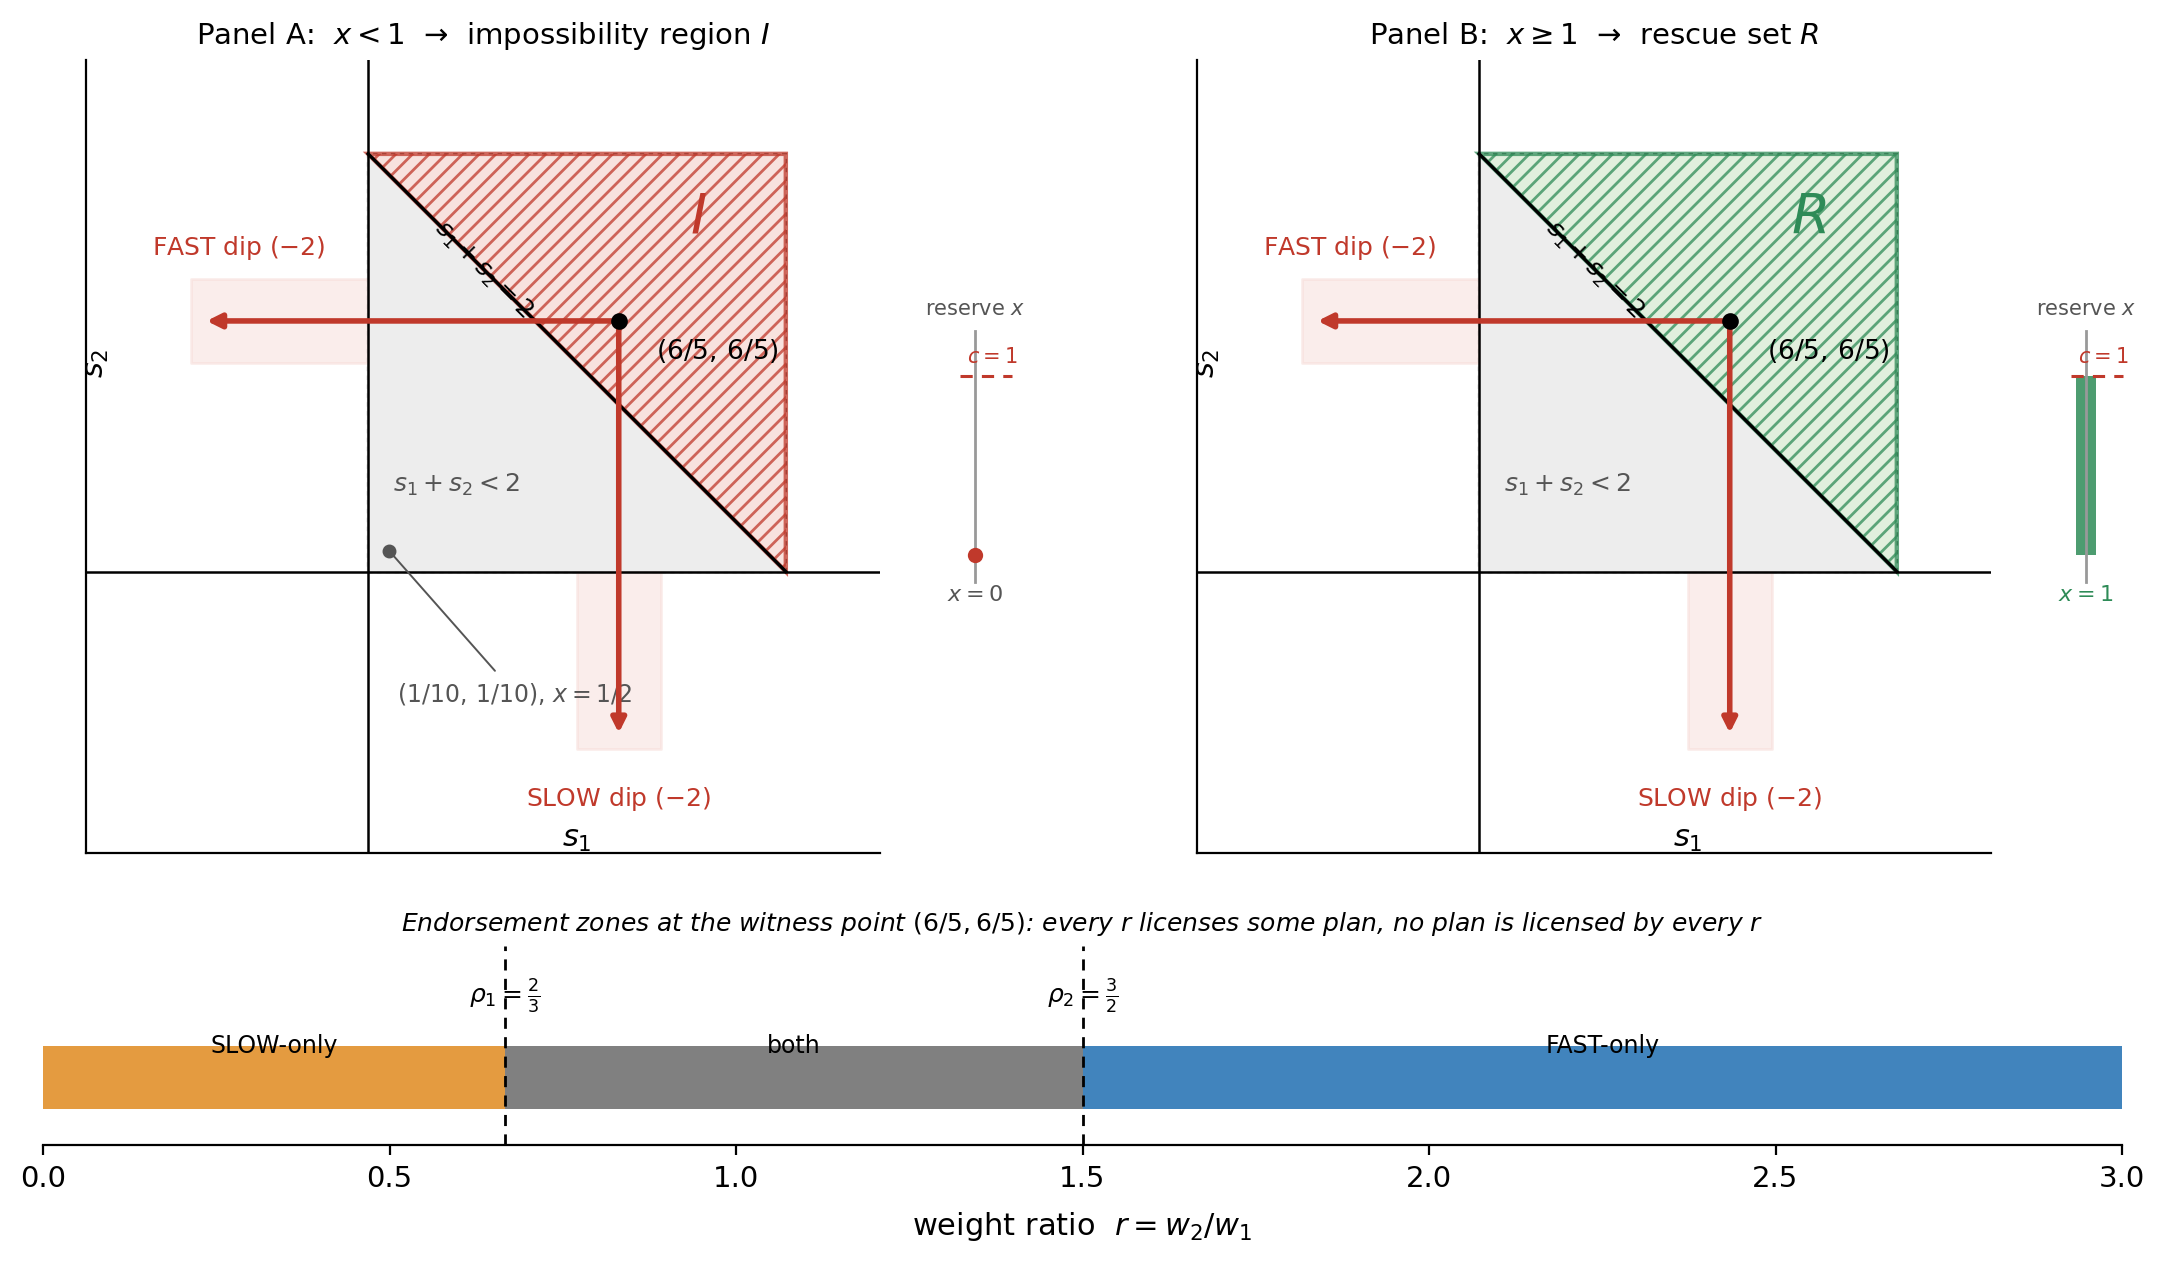
\includegraphics[width=\linewidth]{figs_p1/fig1_witness_v40.png}
\caption{The discrepancy triangle \(\mathcal{Q} = \{ s_1 < 2,\; s_2 < 2,\; s_1 + s_2 \ge 2 \}\) in the floor plane (boundary conventions as in Section 4.6). \textbf{Panel A (\(x < 1\)):} \(\mathcal{Q}\) is the impossibility region \(I = \mathrm{FP}_{\mathrm{agg}}\) --- every weighting licenses a plan, no plan satisfies the floors --- and the worst-case dip arrows show FAST (\(s_1 \to s_1 - 2\)) and SLOW (\(s_2 \to s_2 - 2\)) crossing the zero floors from the witness point \((6/5, 6/5)\). \textbf{Panel B (\(x \ge 1\)):} the same triangle is the rescue set \(R\), served by STAGED. Below the diagonal \(s_1 + s_2 = 2\), both assessments reject when \(x < 1\) and both accept when \(x \ge 1\). The reserve bars show the bridge stock \(x\) against the rescue cost \(c = 1\) (Panel A: \(x = 0\); Panel B: \(x = 1\)). The bottom strip records the endorsement zones at the witness point: SLOW-only for \(r < \rho_1 = \tfrac23\), both for \(\rho_1 \le r \le \rho_2 = \tfrac32\), FAST-only for \(r > \rho_2\). The reserve bars mark representative
slice values (Panel A: \(x = 0\), the impossibility-slice representative;
Panel B: \(x = 1\), at the rescue threshold); the dip arrows are
\(x\)-independent (the floor dynamics do not involve the reserve), and the
canonical witness point of Sections 4.6 and 6.3 sits at \(x = \tfrac12\),
between the drawn slices.}
\end{figure}

\begin{figure}[htbp]
\centering
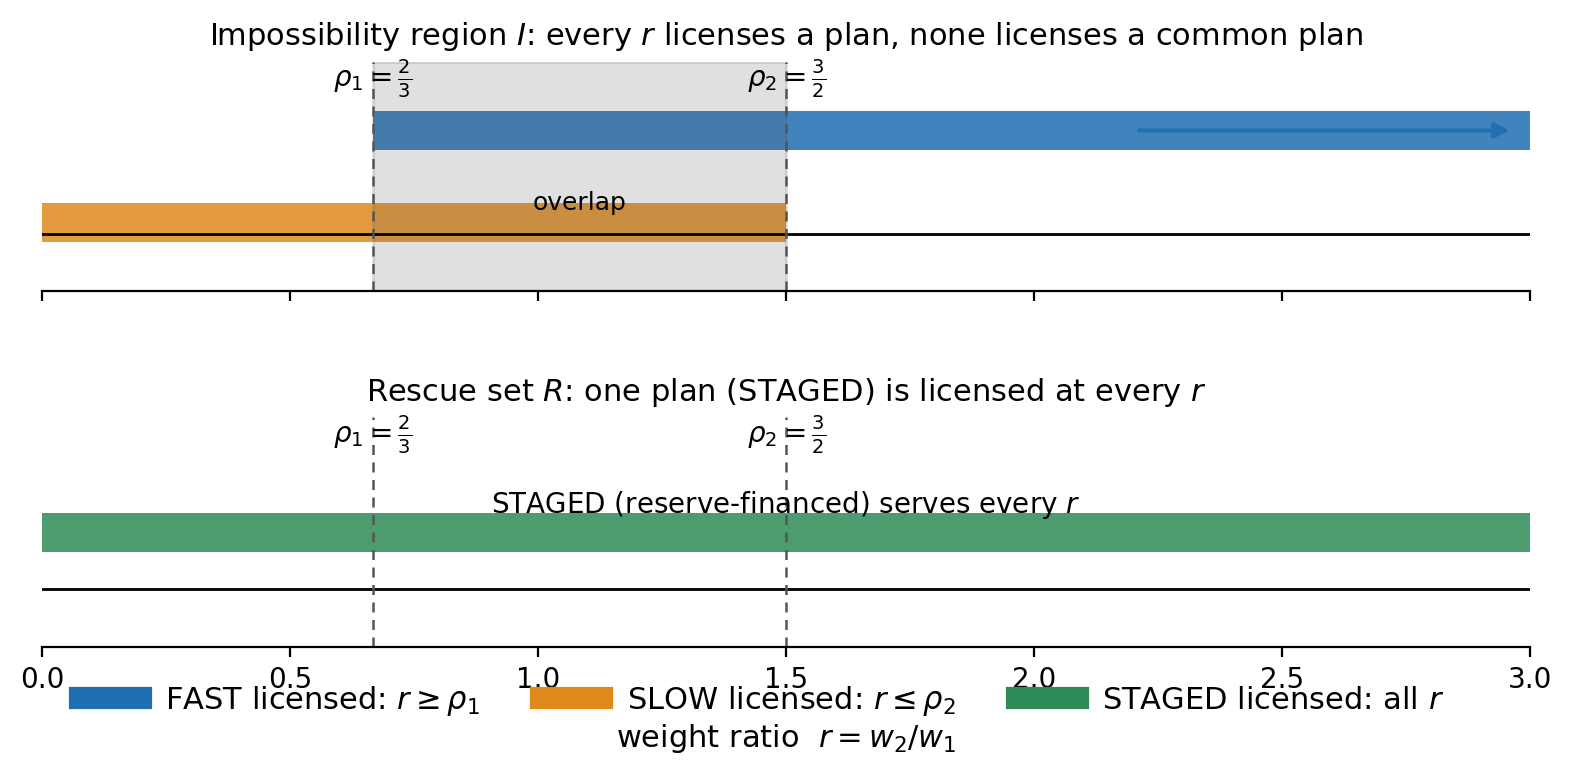
\includegraphics[width=0.98\linewidth]{figs_p1/fig2_weight_intervals_v35.png}
\caption{Weight-interval view at the witness point \((x, s_1, s_2) = (\tfrac12, \tfrac65, \tfrac65)\). FAST is licensed exactly for \(r \ge \rho_1 = \tfrac23\) and SLOW exactly for \(r \le \rho_2 = \tfrac32\). The two intervals together cover every weight ratio \(r \ge 0\), but neither covers it alone: every weight licenses a plan, no plan is licensed by every weight. On the rescue set, STAGED supplies the full interval and closes the gap.}
\end{figure}

\begin{figure}[htbp]
\centering
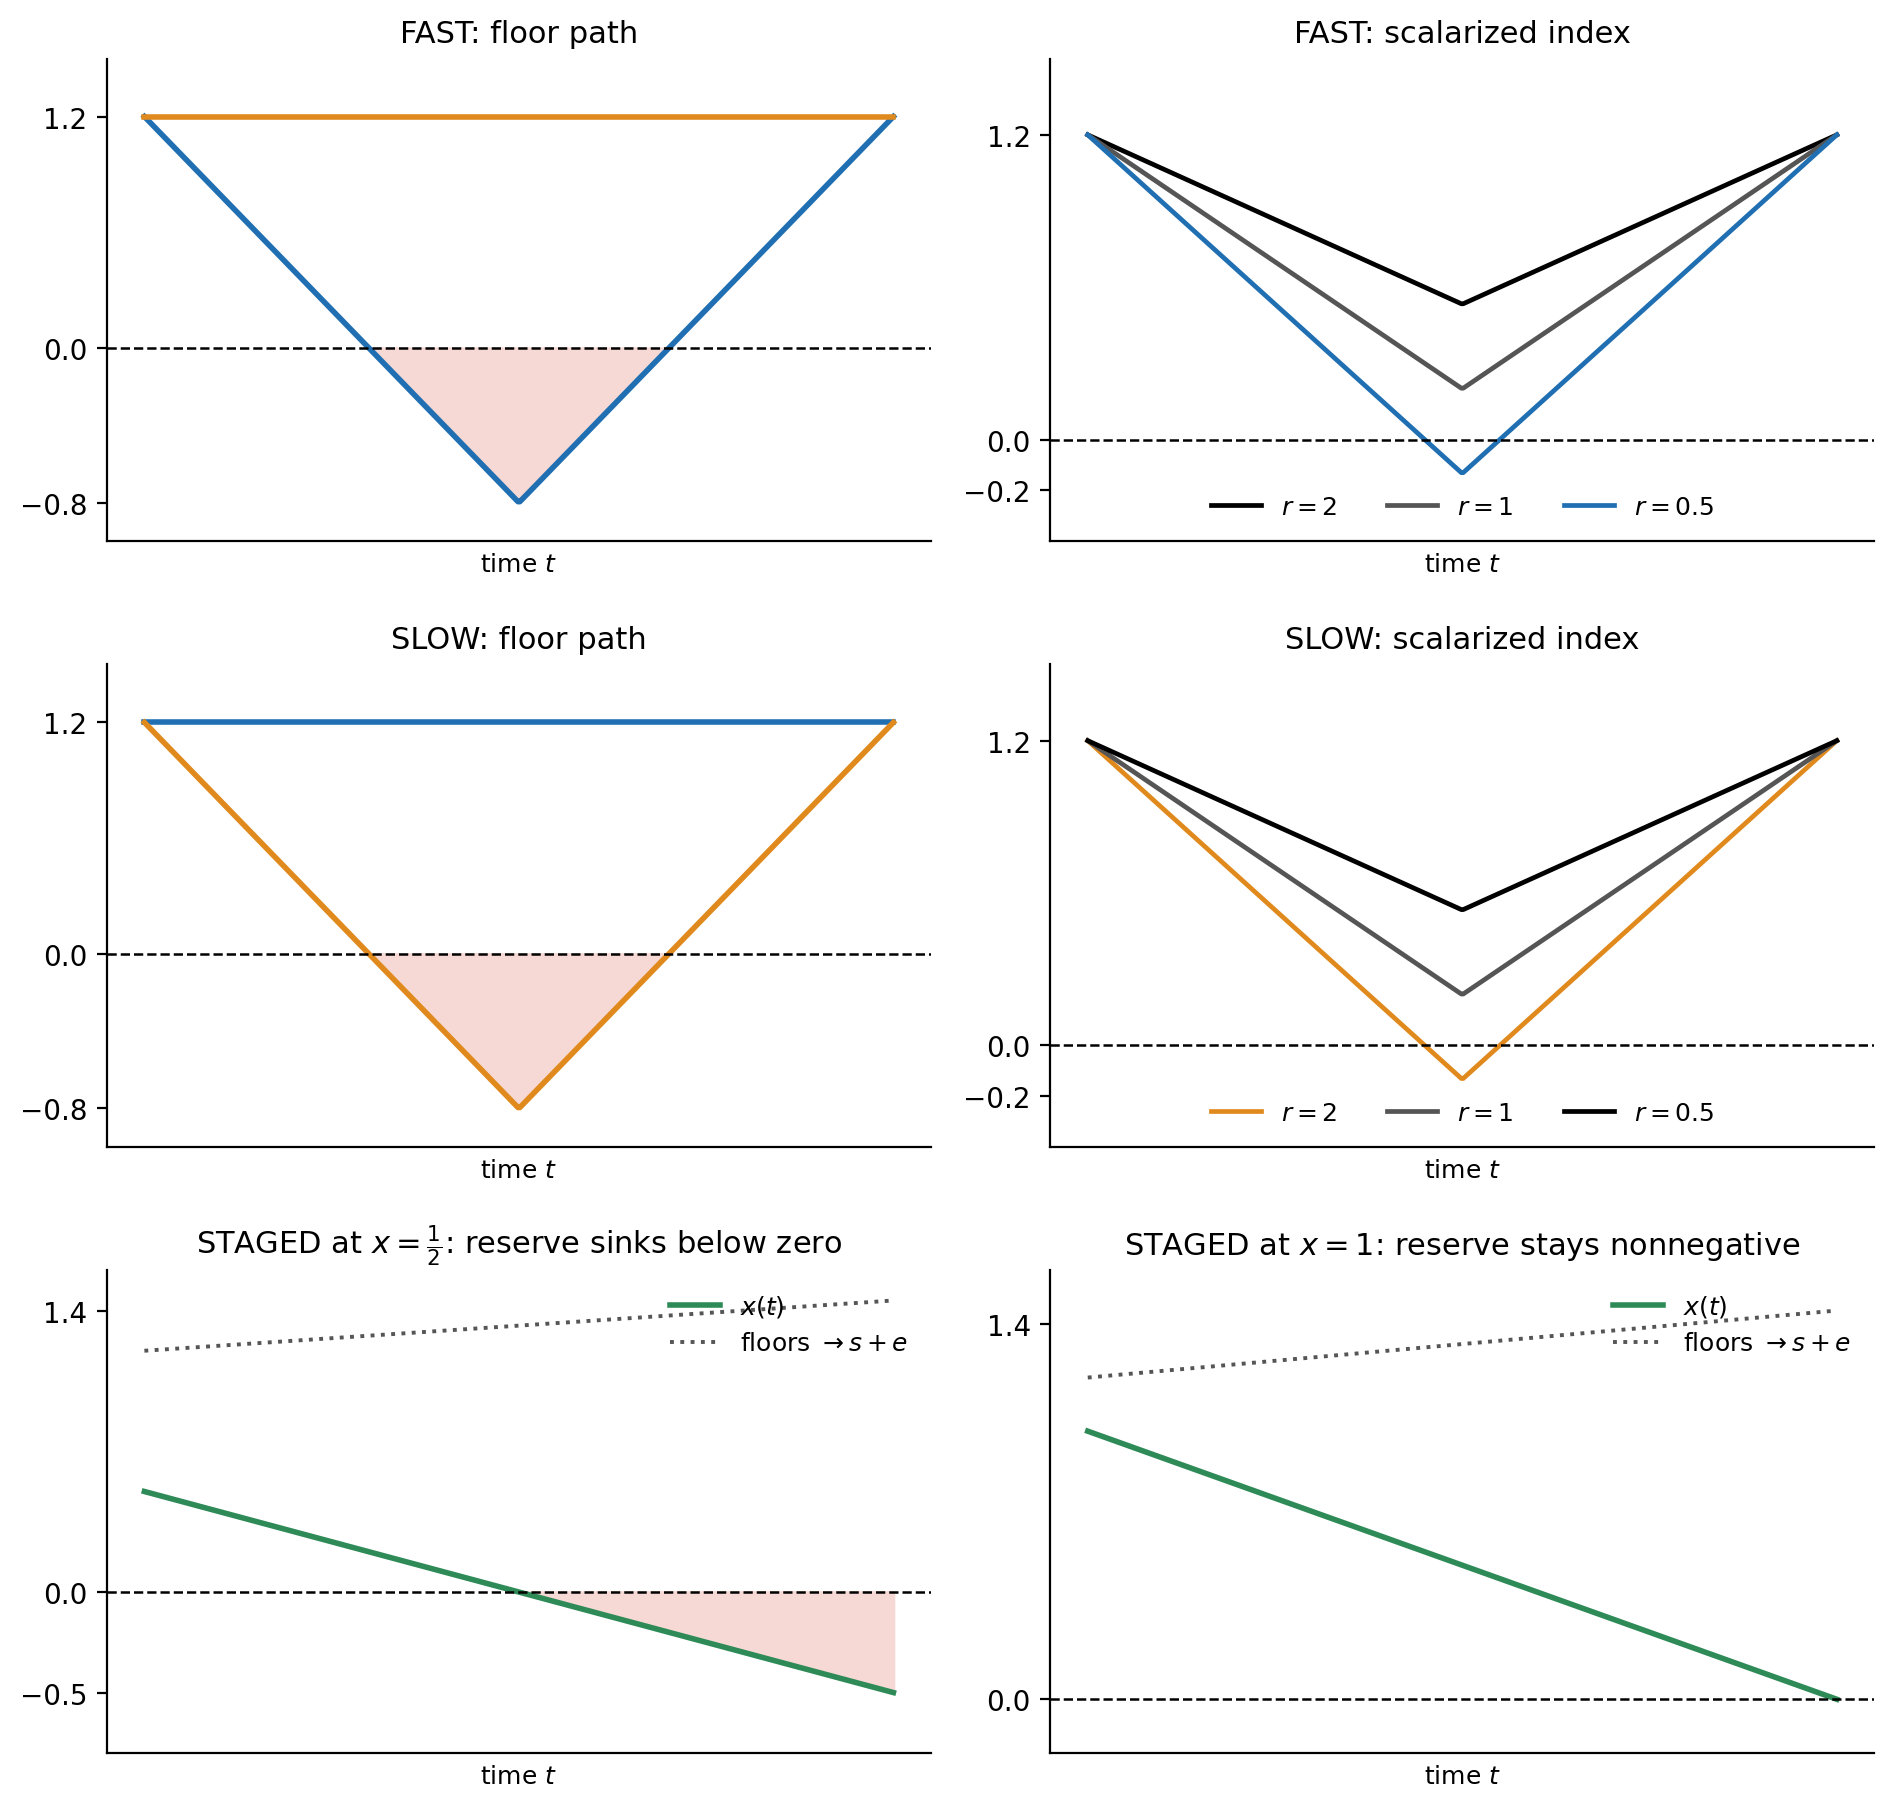
\includegraphics[width=0.98\linewidth]{figs_p1/fig3_path_view_v31.png}
\caption{Path view at the witness point. Rows: FAST, SLOW, STAGED under the worst-case disturbance; solid curves are the constrained paths, the dashed line the zero floor, and the colored curves the scalarized index for \(r \in \{2, 1, \tfrac12\}\). Under FAST (top row) the index stays nonnegative for \(r = 2\) and \(r = 1\) while \(s_1\) breaches its floor; under SLOW (middle row) the mirror holds. The only plan that protects both floors (bottom row, STAGED) consumes the reserve linearly: it is infeasible at \(x = \tfrac12\) and feasible at \(x = 1\), which is what separates the impossibility region from the rescue set.}
\end{figure}

\subsection{Propagation under hold-prefix
extension}\label{sep-propagation-under-hold-prefix-extension}

This subsection asks whether the one-interval separation survives when
the horizon is lengthened by prepending hold intervals. Two results
delimit the answer. Remark 7 establishes persistence under a precisely
specified hold-prefix extension; Theorem 8 exhibits a two-stage datum on
which the gap is erased, showing the persistence claim is
architecture-conditional.

\textbf{Remark 7 (propagation).} \emph{Extend the witness datum to
\(m \ge 2\) review intervals by prepending hold intervals (sole action
HOLD: constant tube \(\{z\}\), successor \(\{z\}\), safe set \(S_0\);
the final interval carries the witness). Assume:}

\begin{itemize}
\tightlist
\item
  \emph{(H1) HOLD is available at every prefix state;}
\item
  \emph{(H2) the hold tube is exactly \(\{z\}\);}
\item
  \emph{(H3) the prefix safe sets contain the witness states;}
\item
  \emph{(H4) terminal and successor architecture labels are unchanged;}
\item
  \emph{(H5) no additional reset or disturbance branches are
  introduced.}
\end{itemize}

\emph{Then:}

\emph{(i) Hierarchy.} \emph{For every stage \(j\),}
\[\mathcal{V}^{\mathrm{typ}}_j \;\subseteq\; \bigcap_{w \in W_+} \mathcal{V}^{w}_j \;\subseteq\; \mathcal{V}^{\mathrm{phys}}_j.\]
\emph{This inclusion holds for every multi-interval typed exact-tube
datum; it is constraint monotonicity under backward induction.}

\emph{(ii) Persistence of strictness.} \emph{The stage-0 accepted
regions are the witness regions pulled back through the holds, so both
strictness witnesses of Theorem 5 persist under this hold-prefix
extension.}

\emph{(iii)} \emph{The displayed separation is not an artifact of the
one-interval framing for the constructed hold-prefixed datum. Strictness
for arbitrary multi-stage systems does not follow without a separate
persistence theorem: a later stage can erase the gap if every
aggregate-feasible state has a common typed-safe continuation, if the
weak and typed terminal sets coincide on the reachable subset, or if
actions couple across stages.}

\emph{Proof.} See Appendix B.

\textbf{Theorem 8 (erasure witness).} \emph{The propagation claim of
Remark 7 is architecture-conditional: there is a two-interval datum
whose single-interval truncation exhibits the acceptance gap and whose
two-stage extension erases it, through the terminal-coincidence
mechanism of Remark 7(iii).}

\emph{Proof.} See Appendix B.

The witness datum of Section 4.5 is not subject to this erasure. Its gap is
tube-driven: on \(I\) every member of the four-action menu violates the
stage-1 path constraint \(S_0\) itself (the two dips and the bridge
deficit of Theorem 5(7)), and a later stage cannot repair a violated
tube --- the stage-1 constraint is local to stage 1. Remark 7's safe
direction is secured by exactly the assumptions the erasure datum
violates (unchanged terminal architecture, no new branches). The two
results together delimit the persistence claim: hold-prefix extension
preserves the separation, arbitrary multi-stage extension does not, and
the erasure mechanisms of Remark 7(iii) are realizable.

\subsection{Machine verification}\label{sep-machine-verification}

Proposition 3, Proposition 4, Theorem 5, Theorem 6, Remark 7, Theorems
8--9, and Proposition 10 are proved in Appendices A--C, and Proposition 11
in Appendix C. An accompanying software artifact (deterministic exact-integer arithmetic; no floating point, tolerances, or randomness) checks the finite rational instance of Proposition 3, Proposition 4, Theorem 5, and Remark 7: the action classifications, the region identities, and the accepted-set identities on a \(31^3 = 29{,}791\)-state grid over \((x, s_1, s_2)\), with a finite verification set containing the critical weight ratios \(\rho_1, \rho_2\) and their midpoint for every enumerated grid state. All 25 checks pass and re-execution reproduces them exactly; they are enumerated in the Supplementary Material (S8). This grid verifier is distinct from the software companion's separate 24-check benchmark suite, which re-derives the Section 6.3 fishery instantiation; the two counts index different check lists, not a disagreement.

\noindent\begin{tabular}{@{}
  >{\raggedright\arraybackslash}p{(\columnwidth - 4\tabcolsep) * \real{0.3333}}
  >{\raggedright\arraybackslash}p{(\columnwidth - 4\tabcolsep) * \real{0.3333}}
  >{\raggedright\arraybackslash}p{(\columnwidth - 4\tabcolsep) * \real{0.3333}}@{}}
\toprule\noalign{}
\begin{minipage}[b]{\linewidth}\raggedright
Claim layer
\end{minipage} & \begin{minipage}[b]{\linewidth}\raggedright
What is established
\end{minipage} & \begin{minipage}[b]{\linewidth}\raggedright
By what
\end{minipage} \\
\midrule\noalign{}
Continuum statements & Exact identities and inequalities on the witness datum & Appendices A--C \\
Finite rational instance & Classifications on the enumerated grid & Deterministic computation \\
Empirical claims & None in this article & --- \\
\bottomrule\noalign{}
\end{tabular}

The finite grid does not by itself prove the continuum identities; it
validates the symbolic classification on the enumerated instance.

A third warrant exists alongside the appendices and the grid. The
appendix proofs of Theorem~5 (1)--(7), Remark~2 with Proposition~3,
Theorem~9 (i) and (iii) with Proposition~10, Lemma~A (the handshake
identity and the engine equivalence), Lemma~B, the master-equation
reductions, and Theorem~S2 are formalized in a mechanized layer
(Lean~4; no axioms, no admitted gaps, no computer-algebra oracle),
every statement being derived from the ordered-field interface alone.
The layer and the appendices were produced independently and agree;
neither is a substitute for the other, and the grid check is a third
and separate thing again --- it validates the symbolic classification
on one enumerated instance, which is all a finite check can do.

\subsection{Menu convexification: the blend
family}\label{sep-menu-convexification-the-blend-family}

The action space is the finite menu \{FAST, SLOW, STAGED,
NO-SWITCH\} of deterministic actions; fractional or alternating policies
are not members of it. The convexification instrument is the blend
family: for each \(\delta \in (0,1)\), the action BLEND\(_\delta\) is
the \emph{convexified action} obtained by fractional allocation of the
primitive control flows,
\(u_\delta = \delta\, u_{\mathrm{FAST}} + (1-\delta)\, u_{\mathrm{SLOW}}\);
by linearity of the flow map its worst-case tube is the pointwise convex
combination of the two primitive worst-case tubes and its successor the
convex combination of the two successors. This is menu convexification
at the level of control inputs --- an explicit model assumption, not the
time-sharing of discrete actions in alternation.


\noindent\textbf{A limitation to state before the theorem.} The blend
family is an explicitly defined convexified control map --- an instrument
of the abstract witness datum, not by itself a claim that fractional plans
are available anywhere. Convexification must be demonstrated from the
model equations (as here, by linearity of the flow map in the control) or
carried explicitly as a management assumption; and a blended control
requires physical and institutional implementability --- fractional
allocation of effort, quota, or seasonal resolution, with monitoring and
enforcement --- before Theorem 9 is applied to a real plan menu. The
theorem is a statement about certification relative to the convexified
menu; the menu's availability is external data (the fourth design test of
Section 5.5 and the instruments of Section 5.6).

\textbf{Theorem 9 (blend collapse).} \emph{On the witness datum of
Section 4.5, over initial states \(X_0\):}

\emph{(i)} \emph{BLEND\(_\delta\) is typed-admissible at \(z\) exactly
when}
\[\delta \in \left[\,1 - \frac{s_2}{2},\; \frac{s_1}{2}\,\right] \cap [0,1],\]
\emph{an interval nonempty exactly when \(s_1 + s_2 \ge 2\) (a singleton
at equality), independent of \(x \ge 0\) and of the weight; the
intersection with \([0,1]\) is the convex-combination domain of
\(\mathrm{BLEND}_\delta\) and is inactive on \(\mathcal{Q}\), where
\(0 < 1 - s_2/2 \le s_1/2 < 1\) automatically.}

\emph{(ii)} \emph{The typed acceptance set of the menu augmented by the
blend family is exactly the compensatory region:}
\[\mathcal{V}_{\mathrm{typ}}^{\mathrm{blend}} \;=\; \{ x \ge 1 \} \cup \{ s_1 + s_2 \ge 2 \} \;=\; \mathcal{V}_{\mathrm{weak}}.\]
\emph{Convexification of the menu collapses the acceptance gap:
\(\mathrm{FP}_{\mathrm{agg}}\) vanishes under the augmented menu, and
the blend family reaches exactly the compensatory region and nothing
beyond --- on
\(\mathcal{V}_{\mathrm{phys}} \setminus \mathcal{V}_{\mathrm{weak}}\) no
blend is typed-admissible.}

\emph{(iii)} \emph{The admissible window depends on the state through
\((s_1, s_2)\) alone: a single \(\delta\) serves every weight
\(w \in W_+\). On the impossibility region the blend is therefore the
common action that no member of the finite menu supplies --- the
acceptance gap is a property of the deterministic menu, not of the
doctrines.}

\emph{Proof.} See Appendix B.

\emph{Remark.} The collapse is exact and weight-independent: a single
convexified plan serves every assessor on \(I\), where the per-weight
plans of Theorem 5(6) necessarily differ. The nonconvexity at work is
menu geometry --- the finiteness and determinism of the action space ---
not the Pareto-frontier geometry under which weighted sums fail to reach nonconvex frontier parts (Das and Dennis, 1997); the two mechanisms are distinct. The structure is precisely that of
pure-versus-mixed strategies in the assessor--planner game (von Neumann,
1928; Sion, 1958): with the planner picking an action, the assessor a
weight, and the payoff the worst-case aggregate, common-plan acceptance
is the pure-strategy value and per-weight acceptance the mixed value,
the gap being the pure-strategy duality gap that the convex (mixed)
extension closes. The two-player reach/avoid formulation of such games is the discriminating kernel of Cardaliaguet (1996), with numerical treatment in Cardaliaguet, Quincampoix, and Saint-Pierre (1999). This is also the here-and-now versus wait-and-see
separation of adjustable robust optimization (Ben-Tal et al., 2004).

\textbf{A class-conditional caveat on the blend collapse.} Theorem 9's
window is computed under the action-indexed disturbance convention of
Section 4.5, and it is class-conditional: under the common-shock class
of Section 5.9 the window is nonempty exactly on \(\{ s_1 \ge \delta,\;
s_2 \ge \delta,\; s_1 + s_2 \ge 3/2 + 2\delta \}\) (at the datum's event
depth \(\delta = 1/2\): \(\{ s_1 \ge 1/2,\; s_2 \ge 1/2,\; s_1 + s_2
\ge 5/2 \}\), against the action-indexed \(\{ s_1 + s_2 \ge 2 \}\) of
Theorem 9(i)). The common-shock acceptance gap --- which survives the
shared shock (Theorem M1, Section 5.9) --- is therefore \emph{not}
blend-closed on the fragile band \(s_1 + s_2 \in [2, 5/2)\): the witness
\((\tfrac12, 1, 1)\) is a common-shock gap state with \emph{no}
admissible blend, while every common-shock gap state with
\(s_1 + s_2 \ge 5/2\) has one (Theorem M3 there; the coupled variant,
by contrast, is blend-closed --- the fragility is class-conditional). An
agency that would otherwise invoke Theorem 9's collapse at a shallow
common-shock gap state cannot: the blended menu itself is inadmissible
there.

\subsection{The converse: discrete time-sharing does not erase
the
gap}\label{sep-the-converse-discrete-time-sharing-does-not-erase-the-gap}

\textbf{Proposition 10 (sequential time-sharing does not erase the gap).}
\emph{On the witness datum of Section 4.5, let a sequential time-shared
policy alternate between FAST and SLOW over the interval, so the set of
visited states is the union of the two primitive worst-case tubes. Then
such a sequential policy is typed-admissible if and only if
\(s_1 \ge 2\) and \(s_2 \ge 2\); on the impossibility region \(I\)
(where \(s_1 < 2\), \(s_2 < 2\), \(s_1 + s_2 \ge 2\)) no such policy is
typed-admissible, and the acceptance gap therefore survives discrete
time-sharing.}

\emph{Proof.} See Appendix B.

\emph{Remark.} Together Proposition 10 and Theorem 9 delimit the notion
of mixing precisely: continuous convexification --- fractional
allocation of control flows --- closes the acceptance gap exactly at the
compensatory region \(s_1 + s_2 \ge 2\), whereas discrete time-sharing
--- alternation in time, whose visited set is the union of the action
tubes --- closes it only where the two dips are independently subsumed,
\(s_1 \ge 2\) and \(s_2 \ge 2\).

On the regime \(s_1 + s_2 \ge 2\) with
\(\min(s_1, s_2) < 2\) (which contains the impossibility region) the gap survives sequential time-sharing and closes only under convexification, so the structural character of the gap is a property of
the \emph{convexity of the action space}, not of the assessment doctrine
and not of temporal sharing as such. A terminological precision is
required here. In the language of relaxed controls, the collapse theorem
is a statement about the convexified (relaxed) action program. The
converse is a statement about discrete, plan-granular alternation at
full strength: each primitive plan is held for a whole sub-interval, so
the visited set is the union of the primitive tubes. That stipulated
visited set is the pointwise worst case over alternation schedules --- a
literal rate-preserving fine-grained alternation visits sub-ranges of it
--- so the impossibility established here is scoped to the worst-case
alternation. It is not a
statement about the chattering limit of classical relaxed-control
theory (Filippov; Warga): infinitesimally fast switching recovers the
convexified trajectory and is therefore subsumed by Theorem 9, not
distinct from it. What fails to erase the gap is alternation at finite
rate and plan granularity, not rapid switching.

\begin{center}\rule{0.5\linewidth}{0.5pt}\end{center}

\section{Interpretation}\label{sep-interpretation}

\subsection{The doctrinal reading}\label{sep-the-doctrinal-reading}

The scalarized operators \(\{E_w\}_{w \in W_+}\) formalize \textbf{one}
compensatory assessment doctrine. The doctrine comprises: a single
aggregate index \(w \cdot s\); nonnegative scalarization weights on
capital forms; substitution across floors permitted at those weights;
and disturbances respected. We refer to this as \emph{the scalarized
aggregate doctrine as formalized here}, not as ``weak sustainability''
simpliciter. The weak-sustainability literature is broader than this
operator: it encompasses aggregate wealth, constant total capital,
nondeclining comprehensive consumption, substitutability assumptions,
discounting, shadow prices, and intertemporal investment conditions
(Neumayer, 2013; World Bank, 2011; Boos, 2015; Dasgupta and M\"aler, 2000;
Asheim, 1994). Likewise, strong sustainability is not always equivalent
to requiring every stock coordinate to remain nonnegative at every
instant. Critical-natural-capital frameworks may use thresholds, safe
operating spaces, irreversibility, resilience, or minimum-service
conditions (Ekins et al., 2003; Rockstr\"om et al., 2009; Raworth, 2012;
Doyen and Gajardo, 2020). The typed
operator \(E_{\mathrm{typ}}\) is a formal idealization of the
separately-binding-floor reading, in the same sense that the scalarized
operators idealize one aggregation doctrine. The typed operator is the
coordinate-wise criterion --- each floor is required to hold separately ---
and the scalarized family is the compensatory criterion; the two vocabularies
name the same operators, with \emph{typed} denoting the framework object and
\emph{coordinate-wise} its constraint structure.

Within this precise scope, Theorem 5 reads as follows. The two
formalized doctrines can disagree on the same transition datum, with the
same robustness standard and the same action set, in the direction
compensatory-accepts / noncompensatory-rejects, on a relatively open
region. The disagreement is not an artifact of one bad weight: every
weight accepts, each licensing a different physical transition. The
plans are genuinely different transitions (FAST and SLOW violate
different floors at different times), which is the dynamic formalization
of substitution across floors. By Proposition 3(ii), the precise seat of
the disagreement is the noncommutativity of ``choose an action'' with
``for all weights.''

At the static level the full-cone aggregate is lossless (Remark 2), so the compensatory doctrine's limitation is not the existence of an aggregate index but the \emph{policy dependence} of the aggregate-feasible transition: the index certifies a set of transitions, none of which the noncompensatory assessment accepts. The two
quantifier orders also carry an information reading.
\(\exists a\, \forall w\) is a commitment made before the weight is
known --- the strong doctrine's robustness demand --- while
\(\forall w\, \exists a_w\) lets the action be chosen after the weight
is observed. On the witness, the acceptance gap between the two orders
measures the value of information about the assessment weight. Theorem 9 qualifies this reading: a single convexified blend serves every weight on the impossibility region, so the value of information reflects the finite deterministic menu rather than the weight information itself. Proposition 10 sharpens the point: the value of information is removed by convexifying the action space, not by sharing actions in time --- under discrete time-sharing the gap (and
hence the value of information about the weight) survives on the
impossibility region.

Throughout, we use ``nonnegative scalarization weights'' for elements of
\(W_+\) and reserve the word ``prices'' for the interpretive discussion.
Actual prices may be strictly positive, endogenous,
dynamically determined, state-dependent, or dimensionally heterogeneous,
and the theorems require none of those properties. The operators are
linear scalarizations with weights fixed over the review interval.
Nonlinear aggregate indices --- CES-type substitutability or endogenous,
state-dependent weighting of the kind that diverges near zero-stock
boundaries --- are different assessment operators, and the theorems
claim nothing for them. Section~\ref{sep-substitutability-spectrum} begins the
programme of establishing what can be claimed for the CES family on the
witness datum.

\subsection{Positioning against established
theory}\label{sep-positioning-against-established-theory}

The backward recursion of Section 3 is
a typed instance of established robust-predecessor, reach-avoid,
capture-basin, and hybrid-reachability constructions (Aubin, 1991;
Aubin, Bayen, and Saint-Pierre, 2011; Saint-Pierre, 1994; Lygeros,
Tomlin, and Sastry, 1999); the fixed-point and algebraic character of these objects is developed in Aubin and Catt\'e (2002). Viability methods are likewise developed in natural-resources management, with fisheries a canonical application (De Lara and Doyen, 2008; Doyen et al., 2012). Proposition 3(i) is constraint-set
monotonicity of viability kernels and reachability sets (Aubin, 1991;
Frankowska, 1989). Static scalarization limitations --- weighted sums that cannot
reach nonconvex parts of Pareto fronts (Das and Dennis, 1997) --- act
through frontier geometry under a single optimization, a mechanism
distinct from the action-quantifier mechanism established here. The
per-literature details --- the commensurability foundation
(Martinez-Alier, Munda, and O'Neill, 1998), the maximin and indicator
formulations of strong sustainability (Martinet, 2011; Cairns and
Martinet, 2014; Doyen and Gajardo, 2020), and the compensability mapping
in multi-criteria decision analysis --- including the outranking approach
PROMETHEE, whose compensatory properties the cited analysis dissects
(Cinelli, Coles, and Kirwan, 2014; Sch\"ar, Pohl, and Geldermann, 2025) --- and the
acceptance-semantics reading of the protocols as decision-aiding
sorting rules (Roy, 1996; Vincke, 1992) --- are collected in the
Supplementary Material (S10).

For multi-criteria decision analysis, the protocols of
Table~\ref{sep-tab:protocols} are acceptance semantics: they specify the rule
by which a composite reading sorts a transition into the accepted or
rejected category --- the sorting problematic of decision aiding (Roy,
1996; Vincke, 1992). The separation is then a statement about which
semantics a composite index can support: under weight-adaptive acceptance
a transition is accepted when every weighting licenses some plan,
possibly a different plan for each weighting, and Theorem 5 exhibits
transitions that this rule accepts and the coordinate-wise rule rejects
on an open region. The licensing thresholds of Theorem 5(6) give the
verdict's exact weight-sensitivity intervals --- the preference ranges
over which each plan is certified --- the acceptance-side analogue of
the sensitivity analyses applied to composite-indicator rankings
(Nardo et al., 2008). Static compensability analyses --- the
compensatory potentials of multi-criteria methods for sustainability
assessment (Cinelli, Coles, and Kirwan, 2014) and the partial
compensability of the outranking approach (Sch\"ar, Pohl, and
Geldermann, 2025) --- classify aggregation behaviour at a fixed profile;
the separation established here acts one level up, in the acceptance
protocol over a transition, and arises even where every static level of
the index is reported correctly (Remark 2).

Against this background, the finite-menu characterization of
Section 4.4 is the general form, of which the witness separation
(Theorem 5) and the blend collapse (Theorem 9) are the instances.

To our knowledge, no explicit exact-tube witness for this dynamic
separation in a compensatory/noncompensatory assessment setting is
reported in the literature. We do not assert priority over the
elementary quantifier fact
\(\exists a\, \forall w \neq \forall w\, \exists a_w\), which is
standard. Whether an equivalent dynamic separation appears in adjacent
literatures (multi-objective robust control, viability theory,
multi-criteria decision analysis) is not established either way.

\subsection{A translation guide for readers from neighbouring
fields}\label{sep-translation-guide}

Because the paper sits at a confluence --- multi-criteria decision analysis
and operations research, control theory and viability, environmental
modelling and governance --- Table~\ref{sep-tab:translation} translates its
central objects into each neighbouring literature's working vocabulary. The
readings are exact correspondences of mathematical role, not analogies: the
theorems are venue-neutral, and a reader may enter through any column.

\begin{table}[htbp]
\centering
\small
\caption{Terminology map: this paper's objects read from three neighbouring
vocabularies.}
\label{sep-tab:translation}
\begin{tabular}{@{}p{2.55cm}p{3.85cm}p{3.55cm}p{4.55cm}@{}}
\toprule
 & \textbf{MCDM / operations research} & \textbf{Control / viability theory} & \textbf{Environmental modelling / governance} \\
\midrule
Typed floors \(s_i \ge 0\), enforced path-wise &
coordinate-wise (vector) criteria; per-criterion lower bounds along the whole path &
state constraints; safe set \(\mathcal{V}\); path (tube) constraints &
planetary boundaries; safe operating spaces; regulatory floors (e.g., a biomass limit reference point) \\
\addlinespace
Scalarized operator \(E_w\) &
weighted-sum acceptance; weight space \(W_+\) &
scalarized robust constraint on an aggregate output &
composite sustainability index; the assessment dashboard \\
\addlinespace
Licensing thresholds \(\rho_1, \rho_2\) &
weight intervals of acceptance; weight-space robustness of a recommendation &
parameter-dependent feasibility margins &
indicator weighting schemes; stakeholder weight elicitation \\
\addlinespace
Acceptance gap \(\mathrm{FP}_{\mathrm{agg}}\) &
scalarization error: accepted by some weighted sum, infeasible coordinate-wise &
gap between the scalarized program and the viability kernel &
the aggregation illusion: an index certifying what the floors reject \\
\addlinespace
Rescue set \(R\); threshold \(\kappa^*\) &
alternatives repairable by a budgeted side payment &
reachability under an auxiliary resource input &
transition finance: adjustment funds, fleet buy-backs \\
\addlinespace
Impossibility region \(I\) &
robust infeasibility: rejected at every weighting &
empty common safe-action set over the belief; kernel exclusion &
hidden collapse zone: index nonnegative, floor crossed mid-transition \\
\addlinespace
Blend collapse (Thm 9) vs.\ time-sharing (Prop 10) &
randomized (mixed) strategies vs.\ deterministic sequencing &
relaxed (convexified) controls vs.\ plan-granular alternation (not the
chattering limit) &
blended policy portfolios vs.\ alternating policies \\
\addlinespace
Exact-tube semantics &
robust path-wise feasibility over a scenario set &
viability tubes; worst-case reachability &
avoiding transient breaches (e.g., extinction vortices during a transition) \\
\bottomrule
\end{tabular}
\end{table}

\subsection{Scope delimitations}\label{sep-scope-delimitations}

\begin{itemize}
\tightlist
\item
  \textbf{No separation on every datum.} Where a single action is safe
  for all weights, the assessments coincide. The theorem is an existence
  separation with an open region, plus the always-valid hierarchy and
  localization.
\item
  \textbf{No infinite-horizon, stochastic, partial-observation, or
  endogenous-event extension.} All statements are for finite-horizon exact-tube data with specified disturbance sets.
\item
  \textbf{No claim that the full nonnegative cone is the only reasonable
  weight family.} Proposition 4 shows that restricting the family
  enlarges the compensatory accepted set, so the full cone is the strictest compensatory reading, and the separation persists a fortiori for restricted families.
\item
  \textbf{No welfare claim about prices.} The weights model an
  assessment doctrine, not a normative endorsement.
\item
  \textbf{No empirical transfer.} The theorems concern assessment operators on a specified datum and imply no empirical claim about any resource system.
\item
  \textbf{No claim that \(\mathcal{V}_{\mathrm{weak}}\) is the
  genuine-savings or inclusive-wealth criterion.} The operator is the
  strictest compensatory reading (every weight, each licensing an
  action). The genuine-savings literature's criterion is a different
  object, and the witness's reserve stock is excluded from the weighted aggregate by construction (Section 4.5), not by consequence of aggregation. If the reserve entered the aggregate with positive weight, the gap could shrink or disappear; the separation isolates the case in which the aggregate measures the service floors while the reserve is a separate policy instrument.
\item
  \textbf{No absolute impossibility.} The impossibility region is a negative certificate relative to the specified four-action menu; with a larger menu it can shrink or vanish (see the completeness requirement in Section 5.7).
\item
  \textbf{No universal doctrinal ranking.} The inclusion
  \(\mathcal{V}_{\mathrm{typ}} \subseteq \mathcal{V}_{\mathrm{weak}} \subseteq \mathcal{V}_{\mathrm{phys}}\)
  is a theorem about the defined operators under common action and
  disturbance classes, common safe-set inclusion, common horizon, common
  tube semantics, and common terminal condition. It does not establish a
  universal ranking of endpoint, weak, and strong sustainability
  doctrines.
\item
  \textbf{No separation under coupled all-floor shocks.} The witness
  disturbance convention is action-indexed (Section 4.5): each action's
  worst case is its own characteristic dip. A datum whose disturbance
  class couples simultaneous dips across all floors of every action
  degenerates the per-weight licensing structure --- the principal
  actions fail together and the compensatory/noncompensatory divergence
  collapses into universal rejection. The exact statement, computed in
  Section 5.9, is reading-conditional and depth-dependent: under the
  additive reading the rejection is universal on \(I\) at the datum's
  full magnitude, with the exact depth boundary \(\delta = 5/4\) below
  which deep-\(I\) states survive (witness \((\tfrac12,
  \tfrac{19}{10}, \tfrac{19}{10})\) at heatwave magnitude) and with the
  separation relocating --- not vanishing --- at full magnitude (the
  coupled gap \(\{ x < 1,\; 2 \le s_1 < \tfrac72,\; 2 \le s_2 <
  \tfrac72,\; s_1 + s_2 \ge \tfrac{11}{2} \}\), witness \((\tfrac12,
  3, 3)\)); under the replace reading the principal actions fail
  together under one weight-independent requirement and what collapses
  is the typed/weak distinction itself (\(\mathcal{V}_{\mathrm{weak}} =
  \mathcal{V}_{\mathrm{typ}}\), Theorem CT there), with acceptance ---
  not rejection --- surviving at \(\{ s_1 \ge 2,\; s_2 \ge 2 \} \cup
  \{ x \ge 1,\; \min(s_1, s_2) \ge \tfrac{15}{8} \}\), a strictly
  more demanding reading (the witness \((\tfrac12, 3, 1)\) is
  action-indexed typed-accepted yet fully rejected under it). The
  separation is exhibited for, and scoped to, the specified
  action-indexed class: the witness datum assumes separable transition risks, with each plan exposing a different floor to its own adverse disturbance. That the coupled regime is not a remote possibility is indicated by evidence that planetary-boundary processes interact and amplify one another (Lade et al., 2020).

\medskip

\noindent The disturbance-class scoping, organized
(Table~\ref{sep-tab:disturbance}): the witness's action-indexed separable
class is one of three regimes; the second's verdict is the common-shock
computation of Section 5.9 (Theorem M1: the gap survives the shared
shock, reduced by the exact \(1/2\)-cut, with licensing thresholds
unshifted on the surviving region) --- a verdict computed, not asserted,
exactly as the regime demands; the third is the universal-rejection
collapse stated above, refined there into two exact reading-conditional
theorems (M4 and CT).

\begin{table}[htbp]
\centering
\small
\caption{Disturbance regimes on the witness datum. The middle row's
verdict is the exact common-shock computation of Section 5.9 (Theorem
M1); the third row's exact statement is reading-conditional (Theorems
M4 and CT there).}
\label{sep-tab:disturbance}
\begin{tabular}{@{}p{3.1cm}p{4.0cm}p{6.3cm}@{}}
\toprule
Regime & Disturbance class & Separation status \\
\midrule
(i) Action-indexed separable & each action's worst case is its own characteristic dip in the coordinate it moves (Section 4.5) & proven: the witness datum exhibits the acceptance gap (Theorem 5) \\
(ii) Common biomass shock & one shared shock strikes the same floor coordinate of every plan & computed (Theorem M1, Section 5.9): the gap \emph{survives} the common shock, reduced by the exact \(1/2\)-cut --- every action-indexed gap state with \(\min(s_1, s_2) < 1/2\) weak-rejects --- with licensing thresholds unshifted on the surviving region; the canonical datum remains a member \\
(iii) Coupled all-floor shocks & simultaneous dips across all floors of every action & reading-conditional (Theorems M4 and CT, Section 5.9): additive --- universal rejection exact on \(I\) at the datum's full magnitude, depth-dependent below the exact boundary \(\delta = 5/4\), the gap relocating (not vanishing) at full magnitude; replace --- the per-weight licensing structure degenerates to one weight-independent requirement, the actions fail together, and the typed/weak distinction itself collapses (\(\mathcal{V}_{\mathrm{weak}} = \mathcal{V}_{\mathrm{typ}}\)), with acceptance --- not common rejection --- surviving (this section; Lade et al., 2020, on boundary interactions) \\
\bottomrule
\end{tabular}
\end{table}

\item
  \textbf{Convexification of the menu.} Fractional action policies are
  not members of the action space, and every stated separation is scoped
  to the finite deterministic menu. Theorem 9 resolves the convexification question: the blend family collapses the typed acceptance set exactly onto the compensatory
  region, so the separation is a property of the deterministic menu, not
  of the doctrines --- menu geometry, distinct from the Pareto-frontier
  geometry of scalarization limits (Das and Dennis, 1997). The
  associated delimitation (Proposition 10) is that discrete time-sharing
  does not effect the same collapse: on the impossibility region the gap
  survives alternation in time, so the structural character of the separation is due to the convexity of the action space, not to temporal sharing.
\end{itemize}

\subsection{Indicator validity: four design tests}\label{sep-indicator-validity}

The separation theorem implies that a composite indicator can be
statically lossless yet dynamically unsound as a
transition-certification device. For indicator developers the theorem
converts into four design tests --- the questions an indicator's
documentation must answer before the index is used to certify a
transition. Each test is a reading of a proved statement; none is a
heuristic.

\begin{enumerate}
\tightlist
\item
  \textbf{Static losslessness.} Does the aggregate preserve component
  violations at a fixed trajectory for the declared weight family? At the
  full cone, yes (Remark 2); for a restricted family, the test is to
  characterize the component violations the restricted family can miss
  (Proposition 4). An index that fails this test fails statically; the
  separation of Section 4 is the further, dynamic failure.
\item
  \textbf{Protocol quantifiers.} Does the certification rule require a
  common plan (\(\exists a\, \forall w\)) or permit weight-adaptive plan
  selection (\(\forall w\, \exists a_w\))? If the latter --- Protocol 2
  of Table~\ref{sep-tab:protocols} --- the indicator is exposed to the
  acceptance gap on exactly the region Theorem 5 exhibits.
\item
  \textbf{Path-wise observability.} Is the index evaluated along the
  full tube, or only at audited endpoints? Endpoint evaluation is the
  weakest operator of the chain (Section 3.1) and cannot detect transient
  breaches --- mid-interval floor crossings that are invisible at
  snapshots (\(E_{\mathrm{end,typ}}\) versus \(E_{\mathrm{typ}}\) on
  the witness datum).
\item
  \textbf{Menu completeness and convexity.} Is the plan menu exhaustive,
  and are blended (convexified) plans implementable? Negative feasibility
  verdicts are menu-relative (Section 5.4), and the gap is a property of
  the deterministic menu that convexification collapses exactly (Theorem
  9, Proposition 10); the availability of the convexified menu is
  external data that the indicator's documentation must declare.
\end{enumerate}

\textbf{A consolidated practitioner checklist.} For an agency using a
composite dashboard to certify a sustainability transition, the four
tests and the theorems behind them operationalize as ten audit points:

\begin{enumerate}
\tightlist
\item
  \textbf{Object of certification:} state what is being certified --- a
  static state, an endpoint, or the existence of a path-wise safe
  management plan.
\item
  \textbf{Binding floors:} list the floors that are legally binding,
  irreversible, or lack verified substitutability; these require
  noncompensatory (Protocol 4) treatment.
\item
  \textbf{Policy quantifier:} declare whether the approval rule assumes
  one robust plan or lets the plan adapt to the weighting.
\item
  \textbf{Weight-dependent plans:} if weight-adaptive, report the
  management plan associated with each relevant weight range (the
  licensing thresholds \(\rho_1, \rho_2\) of Theorem 5(6) are the
  pattern).
\item
  \textbf{Path-wise evaluation:} evaluate the floors along the full
  transition, not only at assessment snapshots (the endpoint operators
  are the weakest of the chain; Section 3.1).
\item
  \textbf{Disturbance structure:} specify whether shocks are common to
  all plans, action-indexed, or correlated across floors
  (Table~\ref{sep-tab:disturbance}); the separation's scope rides on the
  class.
\item
  \textbf{Menu completeness:} acknowledge that negative feasibility
  results are menu-relative unless the action space is demonstrably
  exhaustive (Section 5.4).
\item
  \textbf{Blended policies:} do not infer convexification from
  mathematical convenience; verify that fractional effort or quota
  allocation is administratively implementable (the limitation stated
  before Theorem 9).
\item
  \textbf{Rescue margins:} if a resource-controlled action exists, report
  the minimum increment \(\kappa^*\) that converts impossibility into
  rescue (Section 5.7).
\item
  \textbf{Mandatory reporting:} require that component trajectories and
  their minimum margins be reported alongside the aggregate index, so the
  typed verdict can be independently reconstructed (the minimum report of
  Section 5.6).
\end{enumerate}

\subsection{Policy implications}\label{sep-policy-implications}

The separation theorem has four implications.

\textbf{First.} Aggregate indices alone cannot certify noncompensatory
transition safety under the present assessment semantics. A scalarized
assessment can certify its own criterion --- aggregate feasibility; what
it cannot certify is typed safety unless an additional bridge theorem is
supplied. This follows from Theorem 5: the compensatory accepted set
strictly contains the noncompensatory accepted set, and the excess
region is where the two criteria diverge.

\textbf{Second.} When the typed recursion identifies an admissible
rescue action whose feasibility is controlled by a resource margin,
investment in that margin is a candidate remedy; reweighting alone cannot substitute for it on the witness datum (Section 5.7). This applies where a resource-controlled rescue action exists; it is not a universal policy claim.

\textbf{Third.} Per-floor reporting alongside aggregate reporting is
necessary for detecting this class of discrepancy. It is not universally
necessary for every sustainability judgement; but where the question is
whether a transition respects separately-binding floors, an aggregate
index alone cannot distinguish the rescue region from the impossibility region. The same separately-checked-floor logic underlies the safe-and-just-space (``doughnut'') literature, which evaluates social thresholds and biophysical ceilings independently, without cross-compensation, and reports that no country satisfies all floors within all ceilings (Raworth, 2012; O'Neill et al., 2018; Fanning et al., 2022). A minimum report for such an assessment should include: (1)
typed floors and their provenance; (2) aggregate weights or the weight
family; (3) policy quantifiers; (4) the disturbance set; (5) the
observation and implementation model; (6) exact versus conservative tube
status; (7) terminal maintainability; (8) action-exhaustion status; (9)
uncertainty and approximation bounds; (10) normative premises.

\textbf{Fourth.} Reporting regimes that evaluate endpoints only, as in audited annual snapshots, evaluate only the weakest operator of the chain of Section 3.1. Under those semantics they license transitions that violate typed floors mid-interval without detection (on the witness datum, FAST is typed-endpoint-admissible at every state of \(X_0\) but typed-tube-admissible only for \(s_1 \ge 2\), by inspection of the action table in Section 4.5); the per-floor reporting of the third implication detects the discrepancy. No empirical claim about any particular reporting regime is made here.

The instruments that act on the acceptance gap close it in sharply
different ways; Table~\ref{sep-tab:instruments} records them.

\begin{table}[htbp]
\centering
\small
\begin{tabular}{@{}p{0.22\linewidth}p{0.36\linewidth}p{0.34\linewidth}@{}}
\toprule
Instrument & Mathematical operation & Effect on the gap \\
\midrule
Reweighting & change the weight \(w\) & does not close the gap \\
Restricting the weight family & replace \(W_+\) by \(W \subset W_+\) & enlarges per-weight acceptance; leaves the common-plan problem unless one plan works for all retained weights \\
Reserve augmentation & add STAGED when \(x + \kappa \ge 1\) & closes the gap for states where only the reserve constraint binds \\
Menu convexification & replace \(\mathcal{D}\) by \(\operatorname{conv}(\mathcal{D})\) (the blend family) & closes the gap exactly on the scalarized feasible region \\
Discrete time-sharing & union of the primitive tubes & generally does not close the gap; closes only where both dips are separately survivable \\
\bottomrule
\end{tabular}
\caption{Policy instruments acting on the acceptance gap.}
\label{sep-tab:instruments}
\end{table}

\subsection{Rescue as action synthesis, and data
requirements}\label{sep-rescue-as-action-synthesis-and-data-requirements}

\textbf{Rescue as action synthesis.} Rescue is an operation on the impossibility region. Define a resource-augmentation map
\[\mathsf{Aug}_\kappa : (x, s, \mathcal{A}) \mapsto (x + \kappa,\; s,\; \mathcal{A} \cup \{\mathrm{STAGED}_\kappa\})\]
and the minimal rescue threshold
\[\kappa^* = \inf\{\, \kappa : \exists a \in \mathcal{A}_\kappa,\; a \in E_{\mathrm{typ}}(z) \,\},\]
where \(\mathcal{A}_\kappa\) denotes the augmented menu. \textbf{Proposition 11 (rescue threshold).} \emph{On the witness datum, for every \(z \in X_0\),}
\[\kappa^*(z) = (1 - x)_+ \cdot \mathbf{1}[\,x < 1,\; s_1 < 2,\; s_2 < 2\,] = (1 - x) \cdot \mathbf{1}[\,z \notin \mathcal{V}_{\mathrm{typ}}\,].\]
\emph{Proof.} See Appendix C.

On the impossibility region \(I\), \(\kappa^*(z) = 1 - x > 0\); on the rescue set \(R\), and on all of \(\mathcal{V}_{\mathrm{typ}}\), \(\kappa^*(z) = 0\), matching the observation that states of \(R\) need no augmentation. Because \(\mathrm{STAGED}_\kappa\) is admissible exactly when \(x + \kappa \ge 1\), independently of the floors, the resource route admits every state with \(x < 1\) --- including states outside \(\mathcal{V}_{\mathrm{weak}}\), such as \((\tfrac12, \tfrac1{10}, \tfrac1{10})\) --- at cost \(1 - x\). The set on which the four-action menu fails yet resource augmentation succeeds at finite cost is the full failure set \(\{x < 1,\, s_1 < 2,\, s_2 < 2\}\), which strictly contains the impossibility region; \(I\) is its part on which the aggregate reading still certifies the transition (\(s_1 + s_2 \ge 2\)) --- the genuine acceptance gap of Theorem 5(4). The increment converts any state of the failure set into a typed-transformable one; on \(I\), it converts an aggregate-licensed impossibility into a rescue.

\textbf{The class-conditional rescue trichotomy (a labelled
extension).} Proposition 11's threshold is computed under the
action-indexed disturbance convention of Section 4.5, under which the
resource route is unconditionally finite --- every failure state is
rescuable at cost at most \(1 - x\). The common-shock computation of
Section 5.9 changes this qualitatively: under the common class (a shared
environmental shock of the datum's heatwave magnitude striking every
plan) the threshold becomes a trichotomy (Theorem M2 there) ---
\(\kappa^* = 0\) on the typed accepted set; \(\kappa^* = (1 - x)_+\) on
the failure states with both floors at or above \(3/8\); and
\(\kappa^* = \infty\) on the failure states with \(\min(s_1, s_2) <
3/8\), the first unrescuable-by-reserve failure states on this datum
(witness \((\tfrac12, \tfrac14, 3)\): no reserve increment whatsoever
rescues it, the shared shock's exposure of the staged route's growing
floor exceeding what a floor below \(3/8\) can carry). The canonical
datum's own shortfall is unchanged at \(\kappa^* = 1/2\). The
management reading: at an asymmetric gap state the prescription changes
from reserve accumulation (bridge to \(x = 1\)) to floor rebuilding
(rebuild the weaker floor above \(1/2\) first, above \(3/8\) for the
staged route) --- different actions with different costs and timescales.

\textbf{Institutional forms.} The rescue margin \(\kappa^*(z) = 1 - x\)
maps onto concrete transition-finance instruments: license buy-backs and
vessel decommissioning (the fund spends \(c = 1\) to remove effort),
transition assistance protecting the income floor during the staged
draw-down, and quota banking held against the staged rebuild. The
software companion --- the SafeTransition library --- realizes exactly
this menu on the benchmark datum, as a staged rebuild financed by a fund
buy-back with the rescue threshold truncated at zero once the fund covers
the cost (\(\kappa^* = \max(0,\, 1 - x)\)). The mapping is a reading
aid, not a theorem: each institution must verify its own physical and
legal feasibility before the threshold is read as a financing requirement.

\textbf{Remark (error-bound modulus).} Along the resource route --- varying the reserve \(x\) with the floors held fixed --- the distance to the route's feasible slice \(\{x \ge 1\}\) equals the violation \(f(z) = (1 - x)_+\) itself. The error-bound modulus (Fabian et al., 2010) of this one-parameter relation --- the constant \(\tau\) in \(\mathrm{dist} \le \tau\, f\) --- is therefore identically \(1\): the route is perfectly conditioned. The rescue threshold \(\kappa^*(z) = 1 - x\) coincides with this route-distance, a state-dependent function; the modulus is the constant \(1\) that scales it. On data with nonlinear resource dynamics the distance can cease to equal the violation, and the modulus then governs only the scaling of distance-to-feasibility under unstructured perturbation, a regime outside the present scope (Section 6.2).

\textbf{Data requirements for empirical application.} The theorem is a
result about assessment operators on a specified datum. Empirical
application requires, in addition to the typed floors, disturbance set,
action set, tube model, and destination maintainability witness of
Section 4.5, five further specifications: the completeness status of the
action set (whether \(\mathcal{A}\) is exhaustive or merely a listed
menu), calibration and identifiability data, policy and authority data,
the threshold-uncertainty semantics, and the destination
maintainability status. The itemized requirements are given in the
Supplementary Material (S9).

\subsection{The substitutability spectrum on the witness datum (a
labelled extension)}\label{sep-substitutability-spectrum}

Section 5.1 closes by conceding the nonlinear territory: CES-type
substitutability aggregates are different assessment operators, and the
theorems of Section 4 claim nothing for them. This subsection --- a
labelled extension, not a part of the separation theorem --- begins the
programme of establishing what \emph{can} be claimed, on the witness
datum only, with exact rational witnesses throughout. Its results are
stated on the datum of Section 4.5 and inherit all of its scope
delimitations (Section 5.4); nothing here is an empirical claim.

\textbf{Notation.} Throughout this subsection \(\sigma\) denotes the
elasticity of substitution of a CES aggregate, \(\sigma = 1/(1-\theta)\)
with \(\theta\) the CES exponent. This \(\sigma\) is distinct from
the Schaefer surplus \(\sigma(B)\) of Section 6.3, from the weight
ratios \(\rho_1, \rho_2\) (which are weight quotients, not
elasticities), and from the \(\sigma\)-notations of the companion
papers --- the timing certificate \(\sigma^*(B_0)\) of the
obstruction-calculus companion (Abaee, 2026, \emph{An Obstruction
Calculus for Viability under Incomplete Observation}) and the flow shares
\(\sigma_f, \sigma_c\) of the two-land biocapacity companion (Abaee,
2026, \emph{How Aggregation Can Conceal Composition}).

\textbf{The family.} Work in floor-referenced indices
\(\lambda_i = 1 + s_i\) --- \(\lambda_i = 1\) exactly at the floor,
\(\lambda_i \le 0\) a full floor-unit below it --- the currency in
which geometric-mean abundance indices are defined. For weights normalized
to sum to one, consider the CES/power means
\[M_\theta(\lambda; w) = \Big( \textstyle\sum_i w_i \lambda_i^\theta \Big)^{1/\theta},
\qquad \sigma = \frac{1}{1-\theta},\]
and evaluate Protocol 2 of Table~\ref{sep-tab:protocols} under the
\(\theta\)-aggregate: a state is accepted when, for every weight, some
plan of the Section 4.5 menu keeps \(M_\theta \ge 1\) along its
worst-case tube (the physical and destination constraints are
aggregator-independent; STAGED needs \(x \ge 1\) and then serves every
weight at every rung). Table~\ref{sep-tab:sigmafamily} situates the members.

\begin{table}[htbp]
\centering
\small
\caption{The CES family on floor-referenced indices, on the witness
datum. The linear member is the paper's own engine (Lemma A); the
Leontief member is the typed operator.}
\label{sep-tab:sigmafamily}
\begin{tabular}{@{}llp{7.4cm}@{}}
\toprule
\(\theta\) & \(\sigma\) & reading \\
\midrule
\(1\) & \(\infty\) & the linear aggregate --- the paper's own compensatory engine (Lemma A) \\
\(2/3\) & \(3\) & intermediate CES \\
\(1/2\) & \(2\) & intermediate CES \\
\(0\) & \(1\) & the geometric mean --- the Living Planet Index functional structure (the identification, below) \\
\(-1\) & \(1/2\) & the harmonic mean \\
\(-m\) & \(1/(m+1)\) & the power means below the harmonic member \\
\(-\infty\) & \(0\) & the Leontief minimum --- exactly the typed operator \\
\bottomrule
\end{tabular}
\end{table}

\textbf{Lemma A (the handshake).} \emph{With weights normalized,
\(\sum_i w_i \lambda_i \ge 1 \iff w \cdot s \ge 0\); the
\(\theta = 1\) member therefore reproduces the compensatory engine of
Sections 3--4 exactly --- the same acceptance set at every state and
weight, and at the Section 6.3 datum the same per-weight plan assignment
(the thresholds \(\rho_1 = 2/3\), \(\rho_2 = 3/2\)).} The proof is
the identity \(\lambda_i = 1 + s_i\) and the normalization. The
extension is therefore genuine: it does not move the paper's goalposts;
it interpolates between the paper's operator (\(\sigma = \infty\))
and the typed operator (\(\sigma = 0\)).

\textbf{Lemma B (collapse convention).} \emph{For every \(\theta < 1\)
member, any tube value \(\lambda_i \le 0\) rejects the plan: a
coordinate at or below the collapse level cannot be compensated by
surpluses elsewhere.} The geometric mean is \(0\) there; CES with
\(\theta \le 0\) is undefined there; for \(\theta \in (0,1)\) the
convention is the family's defining property. The \(\theta = 1\) member
alone compensates across collapse --- in itself an exact statement of the
difference between the doctrines: only the perfectly-substitutable
dashboard can certify through a collapsed coordinate.

\textbf{The master equation and the exact ladder.} On the gap-region
diagonal \(z = (x < 1, s, s)\), \(s \in (1, 2)\) --- the Section 6.3
datum sits on it at \(s = 6/5\) --- the cover condition collapses to a
single comparison:

\begin{itemize}
\tightlist
\item
  \(\theta > 0\): accept \(\iff (s-1)^\theta + (s+1)^\theta \ge 2\);
\item
  \(\theta = 0\): accept \(\iff s^2 \ge 2\);
\item
  \(\theta < 0\): accept \(\iff (s-1)^\theta + (s+1)^\theta \le 2\)
  (the inequality flips with the sign of the denominator).
\end{itemize}

Each rung of the ladder then has an exact rational closed form
(Table~\ref{sep-tab:sigmaladder}); every decision is a pure rational
comparison, cross-validated by a second independent code path in the
deposited verifier.

\begin{table}[htbp]
\centering
\small
\caption{The exact closed forms and critical floors of the ladder
(diagonal gap states \(z = (x < 1, s, s)\)). The critical floors are
strictly increasing in depth and converge to the typed boundary \(s = 2\).}
\label{sep-tab:sigmaladder}
\begin{tabular}{@{}lp{4.6cm}p{4.9cm}@{}}
\toprule
\(\theta\) & accept \(\iff\) & critical floor \(s^*(\theta)\) \\
\midrule
\(1\) & \(s \ge 1\) & \(1\) (rational) \\
\(2/3\) & \(s^2 \ge 3\), else \(27(s^2-1)^2 \ge (3-s^2)^3\) & root of \(27(s^2-1)^2 = (3-s^2)^3\), in \((117/100,\, 59/50]\) \\
\(1/2\) & \(s \ge 5/4\) & \(5/4\) (rational) \\
\(0\) & \(s^2 \ge 2\) & \(\sqrt{2}\), in \((141/100,\, 142/100]\) \\
\(-1\) & \(s^2 \ge s + 1\) & the golden ratio \(\varphi = (1+\sqrt{5})/2\) (Fibonacci witnesses: \(8/5\) rejects, \(13/8\) accepts) \\
\(-2\) & \(s^2 \ge 3\) & \(\sqrt{3}\), in \((173/100,\, 174/100]\) \\
\(-m\) & \((s-1)^m + (s+1)^m \le 2(s^2-1)^m\) & increasing in \(m\), brackets in the verifier \\
\(-\infty\) (Leontief) & \(s \ge 2\) & \(2\) --- the typed boundary \\
\bottomrule
\end{tabular}
\end{table}

The critical floors form a strictly increasing ladder
\(1 < 5/4 < \sqrt{2} < \varphi < \sqrt{3} < \cdots \to 2\): the
deeper a state sits in the discrepancy region, the lower the
substitutability needed to expose the breach, and the ladder's collapse
point is exactly the typed boundary. The appearance of \(\sqrt{2}\),
\(\varphi\), and \(\sqrt{3}\) as exact critical floors of the
geometric, harmonic, and \(\sigma = 1/3\) aggregators on this datum
is, to our knowledge, a new exact witness for the substitutability
debate.

\textbf{The critical-elasticity landscape.} For each gap state ---
typed-reject, linear-accept --- the accepted rungs form a prefix of the
ladder (Theorem S1), so there is a critical elasticity \(\sigma^*(z)\):
the \(\sigma\)-aggregator false-certifies \(z\) exactly when
\(\sigma \ge \sigma^*(z)\). Table~\ref{sep-tab:sigmastar} lists exact
brackets on the diagonal \(x = 1/2\).

\begin{table}[htbp]
\centering
\small
\caption{The critical elasticity \(\sigma^*(z)\) on diagonal gap
states \(z = (1/2, s_1, s_2)\) (exact brackets; strict at both ends
unless noted).}
\label{sep-tab:sigmastar}
\begin{tabular}{@{}llp{5.3cm}@{}}
\toprule
state \(z = (x, s_1, s_2)\) & \(\sigma^*(z)\) & note \\
\midrule
\((1/2,\, 1,\, 1)\) & \(\infty\) exactly & only the linear member certifies \\
\((1/2,\, 3/2,\, 1/2)\) & \(\infty\) exactly & min coordinate \(\le 1\): only-linear \\
\((1/2,\, 6/5,\, 6/5)\) & \(\in (2,\, 3)\), strict & the Section 6.3 canonical datum \\
\((1/2,\, 5/4,\, 5/4)\) & \(= 2\) exactly & the \(\theta = 1/2\) rung's equality state \\
\((1/2,\, 13/10,\, 13/10)\) & \(\in (1,\, 2)\) & \\
\((1/2,\, 3/2,\, 3/2)\) & \(\in (1/2,\, 1)\), strict & the LPI-form witness \\
\((1/2,\, 13/8,\, 13/8)\) & \(\in (1/3,\, 1/2)\) & the harmonic member's false-certification witness \\
\((1/2,\, 9/5,\, 9/5)\) & \(\in (1/5,\, 1/4)\) & \\
\((1/2,\, 39/20,\, 39/20)\) & \(\in (1/17,\, 1/13)\) & near the typed boundary: \(\sigma^* \to 0\) \\
\bottomrule
\end{tabular}
\end{table}

The structure on the witness: gap states with \(\min(s_1, s_2) \le 1\)
are only-linear (\(\sigma^* = \infty\)); states with both coordinates
\(> 1\) have finite \(\sigma^*\), given on the diagonal by the
master-equation root, with \(\sigma^*(s) \to 0\) as \(s \to 2^-\)
and \(\sigma^*(s) \to \infty\) as \(s \to 1^+\).

\textbf{Theorem S1 (nesting).} \emph{For every pair of rungs
\(\theta > \theta'\) and every state \(z\), acceptance at
\(\theta'\) implies acceptance at \(\theta\). Consequently the
accepted rungs at each state form a prefix of the ladder;
\(\sigma^*(z)\) is well defined; and it is strictly positive and finite
on every gap state with both coordinates \(> 1\).}

\emph{Proof.} For fixed positive \(\lambda\) and weights,
\(M_\theta\) is nondecreasing in \(\theta\) (the power-mean
inequality); the collapse convention preserves this (acceptance at any
\(\theta' < 1\) forces \(\lambda > 0\) on the serving plan's tube,
where the family is defined). Per plan and weight, hence per weight, hence
for the protocol. Finiteness: on the diagonal, \((s-1)^\theta \to
\infty\) as \(\theta \to -\infty\) since \(s - 1 < 1\), so some
finite \(\theta\) rejects. Positivity: \(s_1 + s_2 \ge 2\) accepts
at \(\theta = 1\). \ensuremath{\square}

\textbf{Theorem S2 (the two-sided Leontief statement).} \emph{(i)
Pointwise: every gap state is safe under some strictly positive
elasticity --- full Leontief is never necessary at a fixed state. (ii)
Uniform: for every \(\theta < 1\) the rung false-certifies an exact
rational interval of gap states (the critical floor \(s^*(\theta) < 2\)
strictly; concretely \(\sigma = 3\) certifies \(s = 6/5\),
\(\sigma = 2\) certifies \(s = 13/10\), \(\sigma = 1\) certifies
\(s = 3/2\), \(\sigma = 1/2\) certifies \(s = 13/8\), and
\(\sigma = 1/4\) certifies \(s = 9/5\)). Hence no positive
\(\sigma\) is uniformly safe on the gap region; the uniform critical
elasticity is \(\inf_z \sigma^*(z) = 0\); and the only uniformly safe
aggregator is \(\sigma = 0\) --- the Leontief member, which is exactly
the typed operator (\(\mathcal{V}^0 = \mathcal{V}_{\mathrm{typ}}\)).}

\emph{Proof.} (i) is Theorem S1's prefix together with acceptance at
\(\theta = 1\) (every gap state is linear-accepted). (ii) Evaluate the
master comparison at \(s = 2\): for \(\theta \in (0,1)\) the
accepting side is \(\ge 2\) and \((s-1)^\theta + (s+1)^\theta = 1 +
3^\theta > 2\) strictly; for \(\theta < 0\) the accepting side is
\(\le 2\) and \(1 + 3^\theta < 2\) strictly --- both strictly
accepting at \(s = 2\), so by continuity some \(\varepsilon > 0\)
has every \(s \in (2 - \varepsilon,\, 2)\) accepted at that rung, and
these are gap states (typed acceptance needs \(s \ge 2\)). The Leontief
member's acceptance is weight-independent (\(\min_i \lambda_i \ge 1\)
does not involve \(w\)), so its protocol collapses into the common-plan
criterion --- the typed operator. \ensuremath{\square}

\textbf{The LPI identification, with its caveats.} The \(\sigma = 1\)
member is the Living Planet Index's functional form --- the geometric mean
of abundance indices --- evaluated here on floor-referenced indices
(\(\lambda_i = 1 + s_i\), so \(\lambda = 1\) at the floor) under the
paper's Protocol 2 quantifier structure. Two caveats state the exact
scope: (a) the LPI's inputs are abundance indices relative to a base
year, not floor margins --- the identification is at the level of the
functional form on the ratio scale, with the floor as reference; (b) the
LPI's operational weighting (equal weights on system-level indices,
chained) is a point in the weight cone, whereas Protocol 2 quantifies
over the whole cone --- the rung decision is therefore the adversarial
version of the LPI reading, and over-, not under-states the index's
exposure. No claim is made that the LPI as published implements Protocol
2.

\textbf{The relevance chain, at the Section 6.3 datum.} The extension
passes the relevance test --- a named decision, a changed indicator
report, a new exact datum, and a changed management action. (1) The
decision: the benchmark's closure decision at the canonical datum, under
a DFO precautionary-approach limit rule. (2) The report flip: at
the canonical trough \(\lambda = (1/5,\, 11/5)\), the linear dashboard
(equal weight) reports \(6/5 \ge 1\) --- certified --- while the
LPI-structured geometric index reports \(\sqrt{11/25} < 1\) (exactly:
\(11 < 25\)) --- a decline signal; the same datum, opposite reports.
(3) The new exact datum: \(\sigma^* \in (2, 3)\) strict at the
canonical state, the algebraic ladder, and the per-rung
false-certification witnesses of Theorem S2(ii). (4) The action flip: at
the canonical datum, every \(\sigma \ge 3\) aggregator certifies --- no
mid-transition LRP response --- while every \(\sigma \le 2\) member
rejects, triggering the mandatory closure and rebuilding response; and at
the witness \((x, s_1, s_2) = (1/2,\, 3/2,\, 3/2)\) the flip is
sharper --- the linear and the LPI-form both certify (no closure) while
the harmonic form rejects, so an agency that replaced its linear
dashboard with the LPI-structured form would still not trigger the
response at this state; the flip requires \(\sigma\) below the state's
critical elasticity \(\sigma^* \in (1/2,\, 1)\), and the triggered
response is concretely the reserve top-up \(\kappa^* = 1 - x = 1/2\)
financing the staged plan (Section 5.7). The aggregator choice --- a
reporting decision, not a management decision --- flips a management
action.

\textbf{Cross-references within the programme.} Two companion results
bracket this extension. The two-land biocapacity study (Abaee, 2026,
\emph{How Aggregation Can Conceal Composition}) establishes the
\emph{composition illusion} --- its continuous-time instance of the
compensatory-aggregation gap, in which a weighted aggregate meets its
floor while the typed floor on ecological capital is violated; Theorems S1
and S2 are the aggregator-side theorems behind that instance. The
obstruction-calculus companion (Abaee, 2026, \emph{An Obstruction
Calculus for Viability under Incomplete Observation}) states the
feasibility-side complement --- its substitution-pathway certificates are
separation certificates, not universal exchange rates --- of which the
present spectrum is the elasticity-side statement.

\textbf{Verification and limits.} Every number in this subsection
is an exact rational, verified in a dedicated fail-loud exact-arithmetic
verifier (57 checks; standard-library fractions only; deterministic; with
a committed byte-reproducible run log) --- a third check list, separate
from and not pooled with the grid verifier's 25 checks and the software
companion's 24 (the programme's non-pooling policy). Two limits are stated.
Off the diagonal, the geometric member's cover comparison is
log-transcendental, and the verifier decides it only on proven sufficient
and necessary rational conditions --- the headline results are diagonal,
so nothing load-bearing rests on the residual undecided cells. And
interior-\(\theta\) values of \(\sigma^*(z)\) are bracketed between
tested rungs --- the brackets are exact and strictness-refined; the
interior value is the master root, transcendental in general.

\textbf{The off-diagonal closure.} Every off-diagonal cell that
the rational conditions leave undecided --- and with it the
complete two-dimensional \(\sigma^*\)-landscape --- is decided by
a dedicated exact computation in the same programme (same datum,
same exactness standard, same delimitations).
The log-transcendental comparison admits no closed form (it has
none); it is \emph{decided}: every verdict below is a finite
rational proof. The device is the \emph{certified rational
enclosure}: every logarithm is bracketed between two rationals
carrying a checkable certificate (the all-positive-term
\(\operatorname{artanh}\) series for \(\ln\), its tail dominated
geometrically), every fractional power by integer \(k\)-th-root
brackets, and every cover comparison below is multilinear in the
enclosed quantities, so that its extrema over the enclosure box
are attained at the vertices --- a finite rational computation.
Under the fail-loud discipline (any cell the schedule cannot decide
aborts the run), zero cells remain undecided.

\textbf{Theorem G (the exact off-diagonal criterion).} \emph{On
the viable gap quadrant --- \(x < 1\), both coordinates in
\((1, 2)\) --- the geometric member's cover comparison reduces,
by cross-multiplication of the two plans' weight thresholds, to}
\[
\mathrm{cover} \iff A \cdot D \le B \cdot C,
\]
\emph{with \(A = \ln(s_1 - 1)\), \(B = \ln(s_2 + 1)\),
\(C = \ln(s_1 + 1)\), \(D = \ln(s_2 - 1)\); equivalently}
\[
r(s_1)\, r(s_2) \le 1, \qquad r(s) = \frac{\ln\bigl(1/(s-1)\bigr)}{\ln(s+1)},
\]
\emph{so the acceptance region is \(\{ s_2 \ge \rho(s_1) \}\),
where \(\rho = r^{-1} \circ (1/r)\) is a strictly decreasing
involution with the unique fixed point \(\rho(\sqrt{2}) =
\sqrt{2}\) (exactly: \(r(s) \le 1 \iff s^2 \ge 2\)) and limits
\(\rho(s) \to 2^-\) as \(s \to 1^+\), \(\rho(s) \to 1^+\) as
\(s \to 2^-\). The pivot has two sides: \(\min(s_1, s_2) \ge
\sqrt{2}\) is sufficient for the cover, and the cover forces
\(\max(s_1, s_2) \ge \sqrt{2}\); the residual wedge \(\{\min <
\sqrt{2} < \max\}\) is split by the curve \(\rho\), which is
transcendental --- bracketed at rational columns with certified
endpoints in the verifier. A coordinate \(s_i \ge 2\) accepts
outright --- its own plan's worst tube keeps both coordinates at
or above \(1\) (\(s_i - 1 \ge 1\) and \(s_j + 1 > 1\)), serving
every weight at every rung --- so the residual decision problem
lives on the open quadrant. For the interior rungs \(\theta \in
(0, 1)\) the same cross-multiplication, applied to the four
powers \(A = (s_1 - 1)^\theta\), \(B = (s_2 + 1)^\theta\),
\(C = (s_1 + 1)^\theta\), \(D = (s_2 - 1)^\theta\), gives the
multilinear form \(F = C (B - 1) + A (1 - D) - (B - D) \ge 0\),
which reduces on the diagonal to the master equation of
Table~\ref{sep-tab:sigmaladder}.}

\emph{Proof sketch (machine-anchored).} FAST's per-weight
acceptance set is the downward interval \([0, U]\), SLOW's the
upward interval \([L, 1]\), with \(U = B/(B - A)\) and \(L =
-D/(C - D)\) at the geometric member (both denominators positive
on the quadrant); the cover is \(L \le U\), and the
cross-multiplication is the criterion. The function \(r\) is
strictly decreasing (its numerator decreasing, its denominator
increasing), so \(\rho\) is well defined and strictly decreasing,
and the criterion's symmetry makes it its own inverse. The
enclosure lemmas certify the four quantities --- and the four
powers --- between rationals; the comparison forms are
multilinear, so the vertex ranges decide; every rejection
additionally carries an exhibited rational witness weight served
by neither plan, cross-validated in both directions against the
independent per-weight algebra. \ensuremath{\square}

\textbf{The residual cells decided.} The two wedge witnesses
certify that the residual was genuine: \((5/4,\, 3/2)\) and its
mirror \((3/2,\, 5/4)\) \textbf{reject}, with certified margins
\(\approx 0.218\) and exhibited rational witness weights served
by neither plan, while \((5/4,\, 7/4)\) and its mirror
\textbf{accept}, with margins \(\approx 0.422\) --- no
per-coordinate rational condition separates them; the curve
\(\rho\) does. Together with the six \((5/4,\, \ge 2)\)-family
cells, accepted by the \(s_i \ge 2\) boundary argument, all ten
undecided cells of the 64-state grid are decided with certified
strict verdicts.

\textbf{The completed two-dimensional landscape.} With the
geometric member decidable off the diagonal and the interior
rungs \(\theta = 1/2\) and \(2/3\) given the same treatment, all
13 rungs are decided at all 64 grid states, with zero cells
undecided: the accepted rungs form a prefix at every state
(Theorem S1's nesting, now machine-complete off the diagonal),
the acceptance regions are up-closed in each coordinate ---
\(\sigma^*(z)\) is nonincreasing in \(s_1\) and in \(s_2\)
(increasing either coordinate raises both plans' worst-tube
aggregates) --- and the diagonal closed forms of
Table~\ref{sep-tab:sigmaladder} are reproduced, the \(\theta = 1/2\)
rung's \((5/4,\, 5/4)\) equality state included. The nine
finite-\(\sigma^*\) states of the core \(\{5/4,\, 3/2,\, 7/4\}^2\)
form clean off-diagonal bands mirroring the diagonal ladder:
\((5/4,\, 3/2)\) and its mirror in \((1,\, 2)\); \((5/4,\, 7/4)\)
and its mirror in \((1/2,\, 1)\); \((3/2,\, 7/4)\) and its mirror
in \((1/3,\, 1/2)\); \((7/4,\, 7/4)\) in \((1/4,\, 1/3)\); the
diagonal \((5/4,\, 5/4)\) is \(= 2\) exactly and \((3/2,\, 3/2)
\in (1/2,\, 1)\), both already in Table~\ref{sep-tab:sigmastar}.
Off-grid specials: \((6/5,\, 7/5)\) and \((13/10,\, 3/2)\) lie
in \((1,\, 2)\). The remaining thirteen gap states of the grid
are only-linear (\(\sigma^* = \infty\), the \(\min(s) \le 1\)
boundary states).

\textbf{Remark (the fixed-sum tolerance structure).} Slice the
gap quadrant by total margin \(s_1 + s_2\) (the anti-diagonals).
The elementary anchors: a slice's balanced point accepts exactly
when \(s_1 = s_2 \ge \sqrt{2}\) (the diagonal closed form), and
the \(s = 1\) edge accepts exactly from total \(3\) up (the
boundary argument); below total \(3\) the near-edge rejects
(\(r \to \infty\) at the edge, against a fixed positive
partner). On the scanned grids the slices assemble into four
regimes:

\begin{itemize}
\tightlist
\item
  \textbf{R1} (totals \(\le 141/50\), the canonical \(12/5\)
  among them): every scanned point rejects --- no asymmetry saves
  the total;
\item
  \textbf{R2} (an interior window, \(141/50 <\) total \(<
  2\sqrt{2}\); exemplar \(707/250\)): the balanced point rejects,
  moderate asymmetry accepts, the edges reject;
\item
  \textbf{R3} (an anchored window, \(2\sqrt{2} \le\) total
  \(< 3\); exemplar \(71/25\)): the balanced point accepts, strong
  asymmetry rejects;
\item
  \textbf{R4} (totals \(\ge 3\)): the whole scanned slice
  accepts.
\end{itemize}

The regime boundaries \(2\sqrt{2}\) and \(3\) are elementary;
the slice-flip total --- where a slice's first accepting point
appears --- is transcendental and machine-bracketed: every
scanned point of the \(141/50\) slice rejects, while the
\(353/125\) slice already contains acceptors, so the flip lies
in \((141/50,\, 353/125]\), strictly below \(2\sqrt{2}\). The
ecological content of the interior window: \emph{moderate
concentration of a deficit is more certifiable than balance} ---
below \(2\sqrt{2}\), the balanced point is not the slice's best
point.

\textbf{The anchor decision: distribution versus total.} The
benchmark's asymmetric-allocation licensing choice fixes the
total margin at \(s_1 + s_2 = 707/250\) (total biomass
\(1707/250\) kt at the Section 6.3 floor \(B_{\mathrm{lim}} = 2\)
kt per stock) and asks how the verdict depends on the allocation
of the deficit across the stocks. Both allocations are gap
states, and the LPI-structured composite rejects the balanced
allocation \((707/500,\, 707/500)\) by the diagonal closed form
--- \((707/500)^2 = 499849/250000 < 2\) exactly, by the exact
excess \(151/250000\) --- while accepting the concentrated
allocation \((607/500,\, 807/500)\) by the certified
log-comparison (\(r\)-product \(\approx 0.9847\), margin
\(\approx 1.17 \times 10^{-2}\)). The same total margin, opposite
verdicts: the false certification of the compensatory dashboard
is visibly two-dimensional --- blind to the \emph{distribution}
of the deficit, not only to its total; the linear dashboard
licenses both allocations, reporting literally the same number,
\(707/500 \ge 1\), on every trough of both states. The report
layer carries the same structure: at the concentrated state,
which stock bears the pulse flips the equal-weight geometric
report --- the FAST-trough \(\sqrt{139849/250000} < 1\), a
decline signal, against the SLOW-trough \(\sqrt{339849/250000}
> 1\), certified --- a plan-design decision with certification
content. And the action layer: the balanced allocation triggers
the mandatory closure and rebuilding response (the reserve top-up
\(\kappa^* = 1 - x = 1/2\) financing the staged plan,
Section 5.7); the concentrated allocation is licensed with no
mid-transition response. The allocation --- a design-level
choice --- flips a management action.

\textbf{Verification (a fifth check list).} Every
number in this closure is an exact rational, verified in a
dedicated fail-loud exact-arithmetic verifier (50 checks;
standard-library fractions only; no floats, tolerances, or
randomness; deterministic; with a committed byte-reproducible run
log) --- a fifth check list, separate from and not pooled with
the grid verifier's 25, the software companion's 24, the
\(\sigma\)-extension's 57, and the common-shock extension's 77
(the programme's non-pooling policy). Limits: the curve \(\rho\), the slice-flip
total, and every interior \(\sigma^*\) value are transcendental
--- the closure provides certified rational brackets, not closed
forms; the slice scans certify the scanned grid points, the
continuum slice-minimum remaining open (the
interval character of the accepting windows is
machine-evidenced, not proved); and the LPI-identification
caveats above carry over unchanged.

\textbf{The continuum slice closure.} The continuum slice-minimum
--- the open residual recorded above --- is decided: a dedicated
exact computation in the same programme (same datum, same
exactness standard, same delimitations) settles the continuum.
The device is the
\emph{\(\phi\)-reduction}: a point \((s, t-s)\) of the total-\(t\)
slice accepts at the geometric member iff
\(\phi(s) := s + \rho(s) \le t\), so the fixed-sum programme is the
sublevel-set programme of one explicit scalar function on
\((1,2)\), with \(\phi(1^+) = \phi(2^-) = 3\) and
\(\phi(\sqrt{2}) = 2\sqrt{2}\). The tangency identity
\(\rho'(s) = -h(s)/h(\rho(s))\), with \(h = r'/r\), makes the
stationary points of \(\phi\) the zeros of
\(D(s) = h(s) - h(\rho(s))\); there are exactly three --- the
elementary fixed point \(\sqrt{2}\), and a tangent pair
\(a^{*} < \sqrt{2} < b^{*}\) with \(\rho(a^{*}) = b^{*}\) and
\(\rho'(a^{*}) = -1\) --- giving the certified four-phase shape of
\(\phi\): descending from the limit \(3\) to its minimum at
\(a^{*}\), rising through \(2\sqrt{2}\), descending to the equal
minimum at \(b^{*}\), climbing back to \(3\). The consequences, each
a certified rational proof:

\begin{itemize}
\tightlist
\item
  \textbf{The slice-flip total.} \(t^{*} = \min_{s\in(1,2)}\phi =
  a^{*} + b^{*} \in (2.82256976476,\, 2.82256976491)\), certified to
  ten places by two independent code paths (the tangency bisection
  on \(D\); the direct slice bisection) --- five orders inside the
  scan bracket \((141/50,\, 353/125]\) and strictly below
  \(2\sqrt{2}\). The flip is attained at the tangent pair, where the
  curve \(\rho\) touches the anti-diagonal:
  \(a^{*} \in (1.14796785390,\, 1.14796785398)\),
  \(b^{*} \in (1.67460191085,\, 1.67460191093)\).
\item
  \textbf{The interval character.} Every accepting window is a
  sublevel interval of one monotone phase of \(\phi\) --- no internal
  holes: the fixed-sum remark's scan-level finding is thereby
  proved.
\item
  \textbf{The total-\(3\) boundary proved in the interior.}
  \(\phi < 3\) on \((1,2)\) --- every interior point of every
  total-\(3\) slice accepts --- and with it the R4 regime wholesale:
  \(\phi(s) < 3 \le t\) for every point of every total-\(t \ge 3\)
  slice.
\item
  \textbf{The harmonic circle.} The \(\theta = -1\) member's
  off-diagonal acceptance region is exactly the exterior of
  \((2s_1-1)^2 + (2s_2-1)^2 = 10\) --- a polynomial identity; the
  circle passes through \((1,2)\), \((\sqrt{2},\sqrt{2})\), and
  \((2,1)\). So nothing at or below \(\theta = -1\) covers anything
  below total \(3\), and the m-side flip total is exactly \(3\),
  attained at the corners --- which every rung accepts.
\item
  \textbf{The \(\sigma^{*}\)-depth sandwich.} Writing
  \(\sigma_{\min}(t)\) for the slice-minimum of the critical
  elasticity, \(\sigma_{\min}(t) \in (1/2,\, 1]\) on
  \((t^{*},\, 3)\) (the circle's strict interior below, the
  \(\phi\)-minimum above); at the anchor total \(707/250\),
  \(\sigma_{\min} \in [12/13,\, 1]\) --- the interior window's best
  point needs nearly full substitutability and lies near the tangent
  branch, sliding toward the corners as \(t\) climbs to \(3\).
  Beyond total \(3\) the corner cusps
  (\(\delta \sim \varepsilon^{m}/m\)) give \(\inf \sigma^{*} = 0\):
  certified rational witnesses at every tested depth \(m\).
\item
  \textbf{The flip-total ladder.} The linear member exactly \(2\)
  (the dashboard identity: cover iff \(s_1 + s_2 \ge 2\));
  \(\theta = 2/3\) exactly \(2\times\)the cubic master root;
  \(\theta = 1/2\) exactly \(5/2\) (the rung's own equality state
  \((5/4, 5/4)\)); \(\theta = 0\) the transcendental \(t^{*}\) ---
  moderate concentration beats balance from the geometric member
  down; every \(\theta = -m\) and the Leontief member exactly \(3\)
  (the circle; the corners). Strictly increasing in depth,
  nesting-consistent.
\end{itemize}

Every number above is an exact rational, verified in a dedicated
fail-loud exact-arithmetic verifier (44 checks; standard-library
fractions only; deterministic; with a committed byte-reproducible run
log) --- a sixth check list, separate from and not pooled with the
five above (the programme's non-pooling policy). Limits: the tangent quantities (\(a^{*}\), \(b^{*}\), \(t^{*}\),
every interior \(\sigma^{*}\)) are transcendental and carry certified
rational brackets only; the four-phase certificate's end segments
rest on value anchors and the elementary asymptotics of \(h\) at the
ends of \((1,2)\), where \(h\) diverges.

\subsection{The common-shock variant of the witness (a
labelled extension)}\label{sep-common-shock-variant}

Section 5.4's disturbance scoping (Table~\ref{sep-tab:disturbance}) leaves the
middle cell --- the common biomass shock, one shared disturbance striking
the same floor coordinate of every plan --- as the one undetermined
verdict: its assertion demands its own exact computation, a common-shock
variant of the witness. This subsection --- a labelled extension in the
sense of Section 5.8, not a part of the separation theorem --- records
that computation and sharpens the coupled regime's row-(iii)
assertion into two exact, reading-conditional theorems. Its results are
stated on the datum of Section 4.5 with only the disturbance class
replaced as specified below; all of Section 5.4's scope delimitations are
inherited; nothing here is an empirical claim.

\textbf{The variant.} Decompose the Section 4.5 datum per the Section 6.3
arithmetic: each principal plan's announced schedule is a mid-interval
tent drawdown of depth \(3/2\) in its characteristic coordinate (FAST:
the quota pulse on \(s_1\); SLOW: the gradual burden on \(s_2\)), the
other coordinate constant; each environmental event is a transient tent
dip of depth \(\delta\) in one floor coordinate, troughing at
\(t = 1/2\) and recovered by \(t = 1\), successors unchanged; the
Section 4.5 worst-case depth \(2 = 3/2 + 1/2\) is the quota pulse plus
the heatwave, so the datum's event depth is \(\delta = 1/2\). STAGED
spends \(x\) (it needs \(x \ge 1\)) while its floors grow linearly
to \(s + e\), \(e = (1/4, 1/4)\); an event of depth \(\delta\) on a
growing floor dips it to \(s + 1/8 - \delta\) --- by
\(\max(0,\, \delta - 1/8)\). The \emph{common} disturbance class
is: the two coordinate events are separate disturbances, each striking
every plan, so each plan's per-coordinate worst case takes its own
schedule plus the event on that coordinate --- ecologically, a marine
heatwave striking the same biomass coordinate regardless of which
harvest-rebuild plan is running. The disturbance quantifier remains
innermost throughout (Section 2.3). One methodological device is used
throughout: STAGED's aggregate dip \(\max(0, \mathrm{raw}(p) - 1/8)\)
is kinked in the weight share \(p = w_1/(w_1 + w_2)\) (with
\(\mathrm{raw}\) affine in \(p\)), and the admissibility requirement
decomposes exactly into the two affine conditions of the kink's two
branches --- every other plan's dip is affine in \(p\) --- so every
cover decision below reduces to exact endpoint evaluations.

\textbf{The handshake.} Before any new class is evaluated, the
computation anchors itself to the deposited datum: under the
action-indexed class of Section 4.5 the variant's machinery reproduces
Theorem 5 exactly --- the same typed and weak acceptance sets, the same
licensing thresholds \(\rho_1 = 2/3\), \(\rho_2 = 3/2\) at the
canonical datum \((\tfrac12, \tfrac65, \tfrac65)\), the same
strictness witness \((\tfrac12, \tfrac1{10}, \tfrac1{10})\) ---
verified on 676 grid states plus the witness list, the same anchoring
discipline as the \(\sigma\)-extension's verifier.

\textbf{Theorem M1 (the middle-cell verdict).} \emph{On the common-shock
variant at the datum's event depth \(\delta = 1/2\):}
\[
\mathcal{V}_{\mathrm{typ}}^{\mathrm{cs}}
= \{ s_1 \ge 2,\; s_2 \ge \tfrac12 \}
\cup \{ s_2 \ge 2,\; s_1 \ge \tfrac12 \}
\cup \{ x \ge 1,\; s_1 \ge \tfrac38,\; s_2 \ge \tfrac38 \},
\]
\[
\mathcal{V}_{\mathrm{weak}}^{\mathrm{cs}}
= \{ x < 1,\; s_1 \ge \tfrac12,\; s_2 \ge \tfrac12,\; s_1 + s_2 \ge 2 \}
\cup \{ x \ge 1,\; s_1 \ge \tfrac38,\; s_2 \ge \tfrac38 \},
\]
\emph{and the acceptance gap survives the common-shock regime:}
\[
\mathrm{FP}_{\mathrm{cs}}
= \mathcal{V}_{\mathrm{weak}}^{\mathrm{cs}} \setminus
\mathcal{V}_{\mathrm{typ}}^{\mathrm{cs}}
= \{ x < 1,\; \tfrac12 \le s_1 < 2,\; \tfrac12 \le s_2 < 2,\;
s_1 + s_2 \ge 2 \}.
\]
\emph{The gap is strictly smaller than the action-indexed impossibility
region \(I\) by the exact \(1/2\)-cut --- every action-indexed gap
state with \(\min(s_1, s_2) < 1/2\) is weak-rejected under the common
class (witness \((\tfrac12, \tfrac1{10}, \tfrac{19}{10})\),
action-indexed weak-accepted by \(s_1 + s_2 = 2\)) --- it is nonempty
with interior, and the canonical datum \((\tfrac12, \tfrac65,
\tfrac65)\) is a member: the compensatory/noncompensatory separation
is not an artifact of the action-indexed convention. On the surviving
region the licensing structure is unshifted: FAST's common-class
licensing endpoint equals its action-indexed endpoint \(1/(1 +
\rho_1)\) at every gap state of the surviving region (SLOW's the
mirror) --- the middle cell's verdict is reduced by the \(1/2\)-cut,
not shifted.}

\emph{Proof sketch (machine-anchored).} Write \(A(p) = p\, s_1 +
(1 - p)\, s_2\) for the aggregate margin at weight share \(p\).
FAST's common-class requirement is \(A(p) \ge \max(2p,\; p +
\tfrac12)\) (its own tent \(3/2\) in \(s_1\) plus the
\(s_1\)-event, and the \(s_2\)-event weighted by \(1 - p\));
SLOW's is the mirror; STAGED's (\(x \ge 1\)) is \(A(p) \ge
\max(p, 1 - p)/2 - 1/8\) (the kink device: the event exposure of a
growing floor). The pointwise minimum of the two principal requirements
is a tent with its only kink at \(p = 1/2\), so an affine \(A\)
covers it exactly at the three abscissae \(p \in \{0, \tfrac12,
1\}\); the closed forms follow. Every constant is an exact rational;
the verifier checks the closed forms against independent grid
computations (5{,}000-state grids for the common class) plus a curated
witness list, both directions, at every grid point. \ensuremath{\square}

\textbf{Theorem M2 (the rescue trichotomy).} \emph{Under the common
class the rescue threshold of Proposition 11 becomes}
\[
\kappa^*_{\mathrm{cs}}(z) =
\begin{cases}
0, & z \in \mathcal{V}_{\mathrm{typ}}^{\mathrm{cs}}, \\[2pt]
(1 - x)_+, & z \notin \mathcal{V}_{\mathrm{typ}}^{\mathrm{cs}},\;
\min(s_1, s_2) \ge \tfrac38, \\[2pt]
+\infty, & z \notin \mathcal{V}_{\mathrm{typ}}^{\mathrm{cs}},\;
\min(s_1, s_2) < \tfrac38.
\end{cases}
\]
\emph{The qualitative change: the resource route fails to rescue every
failure state --- the common shock introduces the first
unrescuable-by-reserve failure states on this datum, with witness
\((\tfrac12, \tfrac14, 3)\): no reserve increment whatsoever rescues
it, the shared shock's exposure of the staged route's growing floor
(\(3/8\)) exceeding what a floor below \(3/8\) can carry. The
canonical datum's shortfall stays \(\kappa^* = 1/2\), its
action-indexed value. The \(3/8\) boundary is proved structurally, not
sampled: the event exposure of a growing floor is \(\max(0, \delta -
1/8) = 3/8\) at the datum's depth, and no floor below it can carry the
event.}

\emph{Proof sketch.} The augmented menu adds
\(\mathrm{STAGED}_\kappa\), admissible at \(x + \kappa \ge 1\)
with the same floor requirement \(s_i \ge 3/8\); \(\kappa\) cannot
move the floors, so on \(\{\min(s) < 3/8\} \setminus
\mathcal{V}_{\mathrm{typ}}^{\mathrm{cs}}\) no finite \(\kappa\)
certifies. On the complement the requirement is the action-indexed one,
\(\kappa = (1 - x)_+\). \ensuremath{\square}

\textbf{Theorem M3 (blend fragility).} \emph{Theorem 9's blend window is
class-conditional: under the action-indexed class at event depth
\(\delta\) it is nonempty exactly on \(\{ s_1 + s_2 \ge 3/2 +
\delta \}\) (Theorem 9 is the \(\delta = 1/2\) instance, \(\{
s_1 + s_2 \ge 2 \}\)); under the common class it is nonempty exactly
on}
\[
\{\, s_1 \ge \delta,\; s_2 \ge \delta,\; s_1 + s_2 \ge \tfrac32 +
2\delta \,\}.
\]
\emph{The common-class gap is therefore not blend-closed on the fragile
band \(s_1 + s_2 \in [2, \tfrac52)\): the witness \((\tfrac12, 1,
1)\) is a common-shock gap state with no admissible blend, while every
common-shock gap state with \(s_1 + s_2 \ge 5/2\) has one. The
coupled gap, by contrast, is blend-closed --- its window threshold and
weak boundary coincide --- so the fragility is class-conditional.}

\emph{Proof sketch.} The blend's \(s_1\)-trough is \(s_1 - \delta -
\delta_{\mathrm{blend}} \cdot \tfrac32\) and its \(s_2\)-trough
\(s_2 - \delta - (1 - \delta_{\mathrm{blend}}) \cdot \tfrac32\)
(each coordinate takes its event plus the corresponding fraction of the
principal tent); the window is the nonnegativity interval of the two,
intersected with \([0,1]\). \ensuremath{\square}

\textbf{Theorem M4 (the coupled regime, additive reading).} \emph{Under
the coupled class --- one disturbance carrying both coordinate events
simultaneously, riding on the plans' own schedules --- at event depth
\(\delta\): the typed accepted set coincides with the common class's
at every depth (the per-coordinate tube minima are event-combination
independent, each coordinate taking its own schedule plus its own
event), and}
\[
\mathcal{V}_{\mathrm{weak}}^{\mathrm{cpl}}
= \{ x < 1,\; s_1 \ge \delta,\; s_2 \ge \delta,\; s_1 + s_2 \ge \tfrac32
+ 2\delta \}
\cup \{ x \ge 1,\; \min(s_1, s_2) \ge \max(0, \delta - \tfrac18) \}.
\]
\emph{At the datum's full magnitude (\(\delta = 2\)) every enumerated
\(I\)-state is weak-rejected --- the Section 5.4 claim holds on the
witness's gap region --- but the claim is depth-dependent with the exact
boundary \(\delta = 5/4\): at heatwave magnitude (\(\delta =
1/2\)) deep-\(I\) states survive as coupled gap states (witness
\((\tfrac12, \tfrac{19}{10}, \tfrac{19}{10})\)), no \(I\)-state
survives at \(\delta \ge 5/4\) while \((\tfrac12, \tfrac{79}{40},
\tfrac{79}{40})\) survives at \(\delta = 5/4 - 1/40\) (every
\(I\)-state has \(s_1 + s_2 < 4\), the survival requirement at
\(\delta = 5/4\)); and at full magnitude the separation relocates
rather than vanishes: the coupled gap}
\[
\{\, x < 1,\; 2 \le s_1 < \tfrac72,\; 2 \le s_2 < \tfrac72,\; s_1 + s_2
\ge \tfrac{11}{2} \,\}
\]
\emph{is nonempty --- the witness \((\tfrac12, 3, 3)\) is
weak-accepted and typed-rejected. ``Universal rejection'' is exact on
\(I\), not global: the divergence re-emerges at larger floors.}

\emph{Proof sketch.} Under the coupled class each plan's aggregate dip
is the sum of both events' weighted contributions (\(3p/2 + \delta\)
for FAST) against the common class's maximum of single-event
contributions; the cover analysis is the tent argument of Theorem M1
with the summed requirements. The boundary: an \(I\)-state has
\(\min(s) < 2\), hence \(s_1 + s_2 < 4\), and survives exactly
when \(s_1 + s_2 \ge 3/2 + 2\delta\), i.e.\ \(\delta \le (s_1 +
s_2 - 3/2)/2 < 5/4\); the witness states realize both sides.
\ensuremath{\square}

\textbf{Theorem CT (the replace-reading collapse).} \emph{Under the
coupled-total class --- the replace reading, each announced-schedule
plan's worst case being the full-magnitude dip \(2\) in each floor,
tent schedules suppressed --- FAST and SLOW degenerate to the same,
weight-independent requirement \(A(p) \ge 2\) (they fail together at
every weight: at the canonical datum both serve nowhere, at
\((\tfrac12, \tfrac52, \tfrac52)\) both serve all of \([0,1]\),
at \((\tfrac12, 3, 1)\) both serve exactly \([\tfrac12, 1]\)),
and}
\[
\mathcal{V}_{\mathrm{weak}}^{\mathrm{ct}} =
\mathcal{V}_{\mathrm{typ}}^{\mathrm{ct}}
= \{ s_1 \ge 2,\; s_2 \ge 2 \} \cup \{ x \ge 1,\; \min(s_1, s_2) \ge
\tfrac{15}{8} \}:
\]
\emph{the typed/weak separation collapses entirely --- the gap is empty
on every state and witness probed --- and the replace reading is
strictly more demanding than the action-indexed class: the witness
\((\tfrac12, 3, 1)\) is action-indexed typed-accepted (\(s_1 \ge
2\)) yet a coupled-total full reject on both tests, as is the canonical
datum itself. The mechanism: the weak test's advantage is weight-wise
plan choice; when every plan faces the same plan- and
weight-independent dip, choice buys nothing, and the per-weight cover
condition degenerates to the same per-coordinate condition the typed
test applies. STAGED's rescue route survives --- its growth mechanics
are not a ``schedule'' in the cost sense; the dip lands on the growing
floor, threshold \(15/8\), exactly its coupled full-magnitude
branch.}

\emph{Proof sketch.} With the tents suppressed and the full dip \(2\)
in each floor, every principal plan's aggregate dip is the constant
\(2\) --- plan- and weight-independent --- so the weak cover condition
\(A(p) \ge 2\) for all \(p\) is the pair of endpoint conditions
\(s_1 \ge 2\), \(s_2 \ge 2\), which is the typed condition;
STAGED's branch is identical under both tests. \ensuremath{\square}

\medskip

\noindent The two readings bracket the coupled truth; both are stated
rather than choosing between them. Two further exact structures complete
the scoping. The \emph{single-event sub-case} (the literal row-(ii)
reading, only the \(s_1\)-event existing) has typed acceptance \(\{
s_1 \ge 2 \} \cup \{ s_2 \ge 3/2,\; s_1 \ge 1/2 \} \cup \{ x
\ge 1,\; s_1 \ge 3/8 \}\), weak acceptance \(\{ x < 1:\; s_1 \ge
1/2,\; s_1 + s_2 \ge 2 \} \cup \{ x \ge 1:\; s_1 \ge 3/8 \}\),
and gap \(\{ x < 1,\; \tfrac12 \le s_1 < 2,\; s_2 < \tfrac32,\;
s_1 + s_2 \ge 2 \}\), the canonical datum a member --- the gap
survives this degenerate class too. And the \emph{\(\delta\)-family}:
all closed forms above are verified at \(\delta \in \{0,
\tfrac14, \tfrac12, 1, \tfrac54, \tfrac32, 2\}\) on cross-section
grids; \(\delta = 0\) degenerates to the benign datum on which all
disturbance classes coincide --- the middle-cell verdict is a genuine
disturbance-structure effect, not a modeling artifact.

\textbf{The relevance chain, at the Section 6.3 datum.} The extension
passes the same four-part test as the \(\sigma\)-spectrum. (1) The
decision: whether a composite biomass index may certify a
stock-rebuilding transition (after the Northern cod case, the Section 6.3
benchmark) when the assessment's disturbance class is a shared
environmental shock --- a marine heatwave striking the same biomass
coordinate regardless of which harvest-rebuild plan is running ---
rather than plan-specific risk; Table~\ref{sep-tab:disturbance} row (ii) at
the canonical datum, with the checklist's sixth audit point demanding
the class be specified. (2) The report flips, on two exact surfaces: the
\(1/2\)-cut (any action-indexed gap state with \(\min(s) < 1/2\)
flips its compensatory verdict from accept to reject --- an index that
certified ``aggregate above 2, transition licensed'' now reports
rejection, witness \((\tfrac12, \tfrac1{10}, \tfrac{19}{10})\)); and
the rescue margin (on \(\{\min(s) < 3/8\}\) the reported
\(\kappa^*\) changes from a finite reserve requirement to infinity
--- ``rescuable with reserve \(\kappa^*\)'' becomes ``not rescuable
by any reserve'', Theorem M2). (3) The new exact datum:
\(\mathrm{FP}_{\mathrm{cs}}\) and its \(1/2\)-cut, the \(3/8\)
rescue boundary, the licensing-invariance identity, the \(5/4\)
coupled boundary with its \(79/40\) witness, the \(11/2\)
relocation gap, and Theorem CT's collapse --- all exact rationals,
machine-anchored. (4) The action flips: at an asymmetric gap state the
action-indexed prescription --- accumulate bridge reserve to \(x =
1\) (\(\kappa^* = (1 - x)_+\)) --- is replaced under a shared-shock
assessment by a floor-targeted action, rebuilding the weaker floor above
\(1/2\) first (above \(3/8\) for the staged route), because no
reserve increment alone certifies (\(\kappa^* = \infty\)); reserve
accumulation and floor rebuilding are different management actions with
different costs and timescales. Second, on the fragile band \(s_1 +
s_2 \in [2, \tfrac52)\), blended quota policies are not admissible
under a shared shock (Theorem M3) --- an agency that would otherwise
blend FAST and SLOW shares at such a state must not.

\textbf{Verification and limits.} Every number in this subsection
is an exact rational, verified in a dedicated fail-loud exact-arithmetic
verifier (77 checks; standard-library fractions only; no floats,
tolerances, or randomness; deterministic; with a committed
byte-reproducible run log) --- a fourth check list, separate from and
not pooled with the grid verifier's 25 checks, the software companion's
24, and the \(\sigma\)-extension's 57 (the programme's non-pooling
policy). Limits: everything is on the witness datum's
decomposition (tent events, exact tubes, the specific STAGED mechanics,
the Section 6.3 arithmetic); no claim about other data beyond the
\(\delta\)-family verified. The two regime-(iii) readings
(additive/replace) bracket the coupled truth; Theorem CT is
reading-conditional, and both are stated rather than choosing. Grid
verification is fail-loud but finite; the closed forms carry proofs
(affine interval arithmetic; the kink device), and the two were
cross-checked against each other at every grid point --- the standard
the \(\sigma\)-extension set. \(\kappa^*\) under the common class
is adjudicated on a reserve grid of step \(1/40\) plus closed-form
confirmation on the survivors; the infinity verdict on \(\{\min(s) <
3/8\}\) is proved structurally, not sampled. No stochastic,
partial-observation, or infinite-horizon claim is made; the disturbance
quantifier remains innermost throughout (Section 2.3).

\begin{center}\rule{0.5\linewidth}{0.5pt}\end{center}

\section{Related work, and what is actually new here}
\label{sep-priorart}

Three literatures run close to this paper. The separation of Section~\ref{sep-results-the-separation-theorem}
is new only in a specific and bounded sense, and the purpose of this section is to state that
sense exactly rather than to claim a wide berth.

\subsection{The scalarization gap in multi-objective optimization}

It is a textbook fact that weighted-sum scalarization recovers only the \emph{supported}
non-dominated outcomes --- those lying on the boundary of the convex hull of the
non-dominated set --- and that no choice of weights recovers unsupported points on
non-convex portions of the front (Koski, 1985; Stadler and Dauer, 1992; Stadler, 1995; Athan
and Papalambros, 1996; Chen, Hansen, Jaumard and Tuy, 1999; Das and Dennis, 1998; Messac and
Mattson, 2002; Huang, Li and Liu, 2007; Miettinen, 1999; Ehrgott, 2005). The remedy
literature --- adaptive weighted-sum schemes, Tchebycheff and weighted-maximization
scalarizations, $\epsilon$-constraint methods --- exists precisely because of it.

Theorem~\ref{sep-the-full-cone-identity}(ii) and Theorem~6(ii) reproduce this geometry exactly:
the scalarized acceptance set is $\operatorname{conv}(\mathcal{D})+\mathbb{R}^n_+$, the
convex hull, and the acceptance gap is its excess over the union of the plans' orthants.
\textbf{The reader should therefore not read the convex-hull characterization as a new fact
about scalarization.} It is the scalarization gap, transported. What is transported, and
what is not, is the subject of Section~\ref{sep-whatisnew}.

\subsection{Adjustable and randomized robust optimization}

Robust optimization distinguishes the robust counterpart, in which all decisions are
here-and-now, from the adjustable robust counterpart, in which a second stage may respond to
realized uncertainty (Ben-Tal, Goryashko, Guslitzer and Nemirovski, 2004, \emph{Mathematical
Programming} 99(2), 351--376; Ben-Tal, El Ghaoui and Nemirovski, 2009). Ben-Tal et al. note
that under constraint-wise uncertainty the two coincide for linear problems, and Bertsimas
and Goyal (2012) characterize when static and adjustable solutions agree. The analogue of
the present quantifier inversion --- a single plan for all weights against a plan per
weight --- is therefore structurally familiar in that literature.

Separately, it is well established that \emph{randomizing} over decisions can strictly
improve worst-case performance against a deterministic choice: this is the content of the
mixed-strategy and complete-class results of statistical decision theory, and it has been
revisited in robust optimization, where problems are classified as randomization-receptive
or randomization-proof according to whether a randomized decision strictly beats the
deterministic optimum (Krause, Singla and Golovin, 2011; Vorobeychik and Li, 2014; Sinha,
Fang, An and Kiekintveld, 2018; Sessa, Bogunovic, Kamgarpour and Krause, 2020; Kobayashi and
Takazawa, 2023). Theorem~9 --- that admitting fractional blends closes the aggregate-certified
gap exactly --- sits in this line.

\subsection{Weak and strong sustainability}

The distinction this paper formalizes is the one environmental economics draws between weak
sustainability, under which natural and manufactured capital are substitutes and only the
aggregate need be maintained, and strong sustainability, under which critical natural
capital is non-substitutable and must be maintained separately (Pearce and Atkinson, 1995;
Daly, 1995; Beckerman, 1994; Ayres, 1996; Neumayer, 2003; the critical-natural-capital
literature surveyed in Dietz and Neumayer, 2007). That debate is largely conducted in
verbal and policy terms. It has not, to our knowledge, been given a separation theorem with
an exact witness, and the practical maxim advanced here --- that where floors bind
separately, reporting them individually is a detection requirement rather than a
presentation preference --- is a consequence of the formal result rather than a restatement
of the policy position.

\subsection{What is claimed as new}
\label{sep-whatisnew}

Given the above, the contribution is deliberately narrow. We claim four things and nothing
more.

\begin{enumerate}
\item \textbf{The setting.} The separation is established for \emph{robust transition safety
over a finite horizon with path-wise constraints}, not for the recovery of Pareto points by
a scalarized optimization. The objects compared are acceptance \emph{sets of states} under a
viability constraint, and the argument turns on quantifier order in that setting. The
multi-objective literature asks whether a weighted-sum optimizer can \emph{reach} an
unsupported point; we ask whether a \emph{transition certified by every weighting} is
implementable at all.

\item \textbf{The negative result on time-alternation, which inverts the usual ordering.}
Theorem~9 shows that fractional blending closes the gap exactly, while alternating between
plans over time does not. In robust optimization the ordering runs the other way:
adjustability weakens conservatism, so the adjustable counterpart dominates the static one.
Here convexification in \emph{plan space} achieves what open-loop variation over
\emph{time} cannot. We have not found this comparison, or this inversion, in the robust
optimization or randomization literatures surveyed above, which study worst-case
\emph{objective value} rather than path-wise \emph{feasibility}. This is the sharpest claim
in the paper and the one most likely to be contested.

\item \textbf{The detection reading.} Because the gap has nonempty interior on an explicit
datum, an aggregate index cannot distinguish the rescuable from the impossible without a
separate check of the floors or a verified common implementable plan. That is a statement
about what a reported index can and cannot certify, and it is a consequence of (i) and (ii),
not an independent assertion.

\item \textbf{The witness.} The datum is realized in exact rational arithmetic with a
fishery transition under a heatwave disturbance, units anchored to a regulated biomass
limit, with the gap a region of nonempty interior rather than a measure-zero boundary
phenomenon.
\end{enumerate}

\noindent We do \emph{not} claim the quantifier-order observation itself (Remark~1 is
elementary order theory), the convex-hull geometry (it is the known scalarization gap), or
the usefulness of randomization under worst-case objectives (well established). A reader
familiar with any of the three literatures above will recognize the ingredients; the claim
is about the specific object they assemble here and, principally, about item 2.

\section{Discussion}\label{sep-discussion}

\subsection{Negative certificates}\label{sep-negative-certificates}

A negative certificate --- a rejection with an exhibited violated constraint for each action, exhausting the action set --- is a complete verdict, not an inconclusive one. Theorem 5(7) is an instance: four actions, four exhibited violations, certifying impossibility on \(I\) together with the resource threshold of Section 5.6 and the per-weight licensing thresholds of Theorem 5(6). Related scored forecast-evaluation studies apply assessment discipline of the same kind to the Northern cod and Edwards Aquifer systems (Abaee, 2026, \emph{Does a Surplus-Production Ladder Improve Forecasts of Northern Cod?}; Abaee, 2026, \emph{Does a One-Pool Water-Balance Model Improve Forecasts of Edwards Aquifer Head?}); the cited studies are referenced for related work only.

\subsection{Limitations}\label{sep-limitations}

\begin{enumerate}
\def\labelenumi{(\roman{enumi})}
\tightlist
\item
  The separation theorem is an existence result with an open region; it does not imply the gap is large in any given application, and where the assessments coincide it yields nothing.
\item
  Novelty statements reflect bounded literature search (Section 5.2).
\item
  The operators cover finite horizons with exact tubes and specified disturbance sets; infinite horizons, partial observation, stochastic chance constraints, and endogenous event times are not treated.
\item
  The finite-menu theorem of Section 4.4 governs plans whose admissibility is characterized by a required-margin vector; plans outside that class (reserve-financed plans, destination-failing plans) are handled separately, and the geometric form of the gap is established within the margin class.
\item
  If a convexified (blended) plan is physically and institutionally available, the gap disappears by Theorem 9; the separation is therefore a statement about certification relative to the available plan menu, not a claim that the gap is unavoidable in every institution.
\item
  Conservatism of the benchmark's certified tubes (Section 6.3) is
  regime-conditional: the exact inequality that makes the tubes
  conservative uses the Schaefer surplus's monotonicity below \(K/2\).
  Depensation in the stock--recruitment relationship, or heatwave
  mortality amplified nonlinearly at low stock, would reduce the recovery
  surplus, and the certified tubes would then no longer be conservative
  for the nonlinear realization; the certification statements of
  Section 4, which concern the datum rather than the realization, are
  unaffected.
\item
  No empirical claims are made.
\item
  The governance, intergenerational, and composition extensions are stated at partial status in the Supplementary Material and are not used in the proofs.
\item
  Computational tractability: on a finite explicit state--action--disturbance graph with constant-time predicate evaluation, the backward recursion is polynomial in the graph size and horizon. For continuous, hybrid, or belief-state models, the graph itself may be exponentially large, infinite, or only approximately representable; exact-tube inclusion may be computationally hard or undecidable; and grid cardinality grows as \(N_{\mathrm{grid}} = \prod_{i=1}^n N_i\) --- exponentially in dimension when floors are coordinates. The witness is tractable because its datum is small, finite, and rational.
\item
  The off-diagonal closure of Section~\ref{sep-substitutability-spectrum}
  decides every cell of the 64-state grid by finite rational proof,
  not closed form: the curve \(\rho\), the slice-flip total, and
  interior \(\sigma^*\) values are transcendental and carry
  certified rational brackets only.
\item
  The \(\sigma\)-extension of Section~\ref{sep-substitutability-spectrum}
  states two limits. Off the diagonal, the geometric
  member's cover comparison is log-transcendental, and the
  verifier decides it only on proven sufficient and necessary
  rational conditions --- the headline results are diagonal, so
  nothing load-bearing rests on the residual undecided cells;
  the off-diagonal closure decides every such cell by finite
  rational proof. And interior-\(\theta\)
  values of \(\sigma^*(z)\) are bracketed between tested rungs
  --- the brackets are exact and strictness-refined; the interior
  value is the master root, transcendental in general.
\item
  The common-shock extension of Section~\ref{sep-common-shock-variant}
  states its limits: everything is on the witness datum's
  decomposition (tent events, exact tubes,
  the specific STAGED mechanics, the Section 6.3 arithmetic);
  no claim about other data
  beyond the \(\delta\)-family verified. The two regime-(iii)
  readings (additive/replace) bracket the coupled truth ---
  Theorem CT is reading-conditional, and both are
  stated rather than choosing. Grid verification is
  fail-loud but finite, the closed forms carry proofs
  (affine interval arithmetic; the kink device), and the two
  were cross-checked against each other at every grid point
  --- the standard the \(\sigma\)-extension set. \(\kappa^*\)
  under the common class is adjudicated on a reserve grid of
  step \(1/40\) plus closed-form confirmation on the survivors,
  and the infinity verdict on \(\{\min(s) < 3/8\}\) is
  proved structurally, not sampled; no stochastic,
  partial-observation, or infinite-horizon claim is made, and
  the disturbance quantifier remains innermost throughout
  (Section 2.3).
\item
  The continuum slice-minimum of the fixed-sum tolerance structure
  --- where a slice's best point lies --- is closed (the continuum
  slice closure of Section~\ref{sep-substitutability-spectrum}): the
  slice-flip total is certified at \(t^{*} = a^{*} + b^{*}\) --- the
  tangent pair of the boundary involution --- to ten places, by two
  independent code paths; the accepting windows are intervals (each
  a sublevel interval of a monotone phase of \(\phi = s +
  \rho(s)\)), so the interior window's ecological content (moderate
  concentration of a deficit is more certifiable than balance) is
  certified on the continuum, not only at the scanned points; the
  total-\(3\) regime boundary is proved in the
  interior (\(\phi < 3\)); the harmonic member's region is exactly
  the circle \((2s_1-1)^2 + (2s_2-1)^2 \ge 10\), so nothing at or
  below \(\theta = -1\) covers below total \(3\) and the m-side flip
  total is exactly \(3\); \(\sigma_{\min}(t) \in (1/2,\, 1]\) on
  \((t^{*},\, 3)\), with \(\sigma_{\min}(707/250) \in [12/13,\, 1]\)
  and \(\inf \sigma^{*} = 0\) beyond total \(3\) (corner cusps). The
  transcendental quantities (\(a^{*}\), \(b^{*}\), \(t^{*}\), the
  interior \(\sigma^{*}\) values) carry certified rational brackets
  only.
\end{enumerate}

\begin{figure}[htbp]
\centering
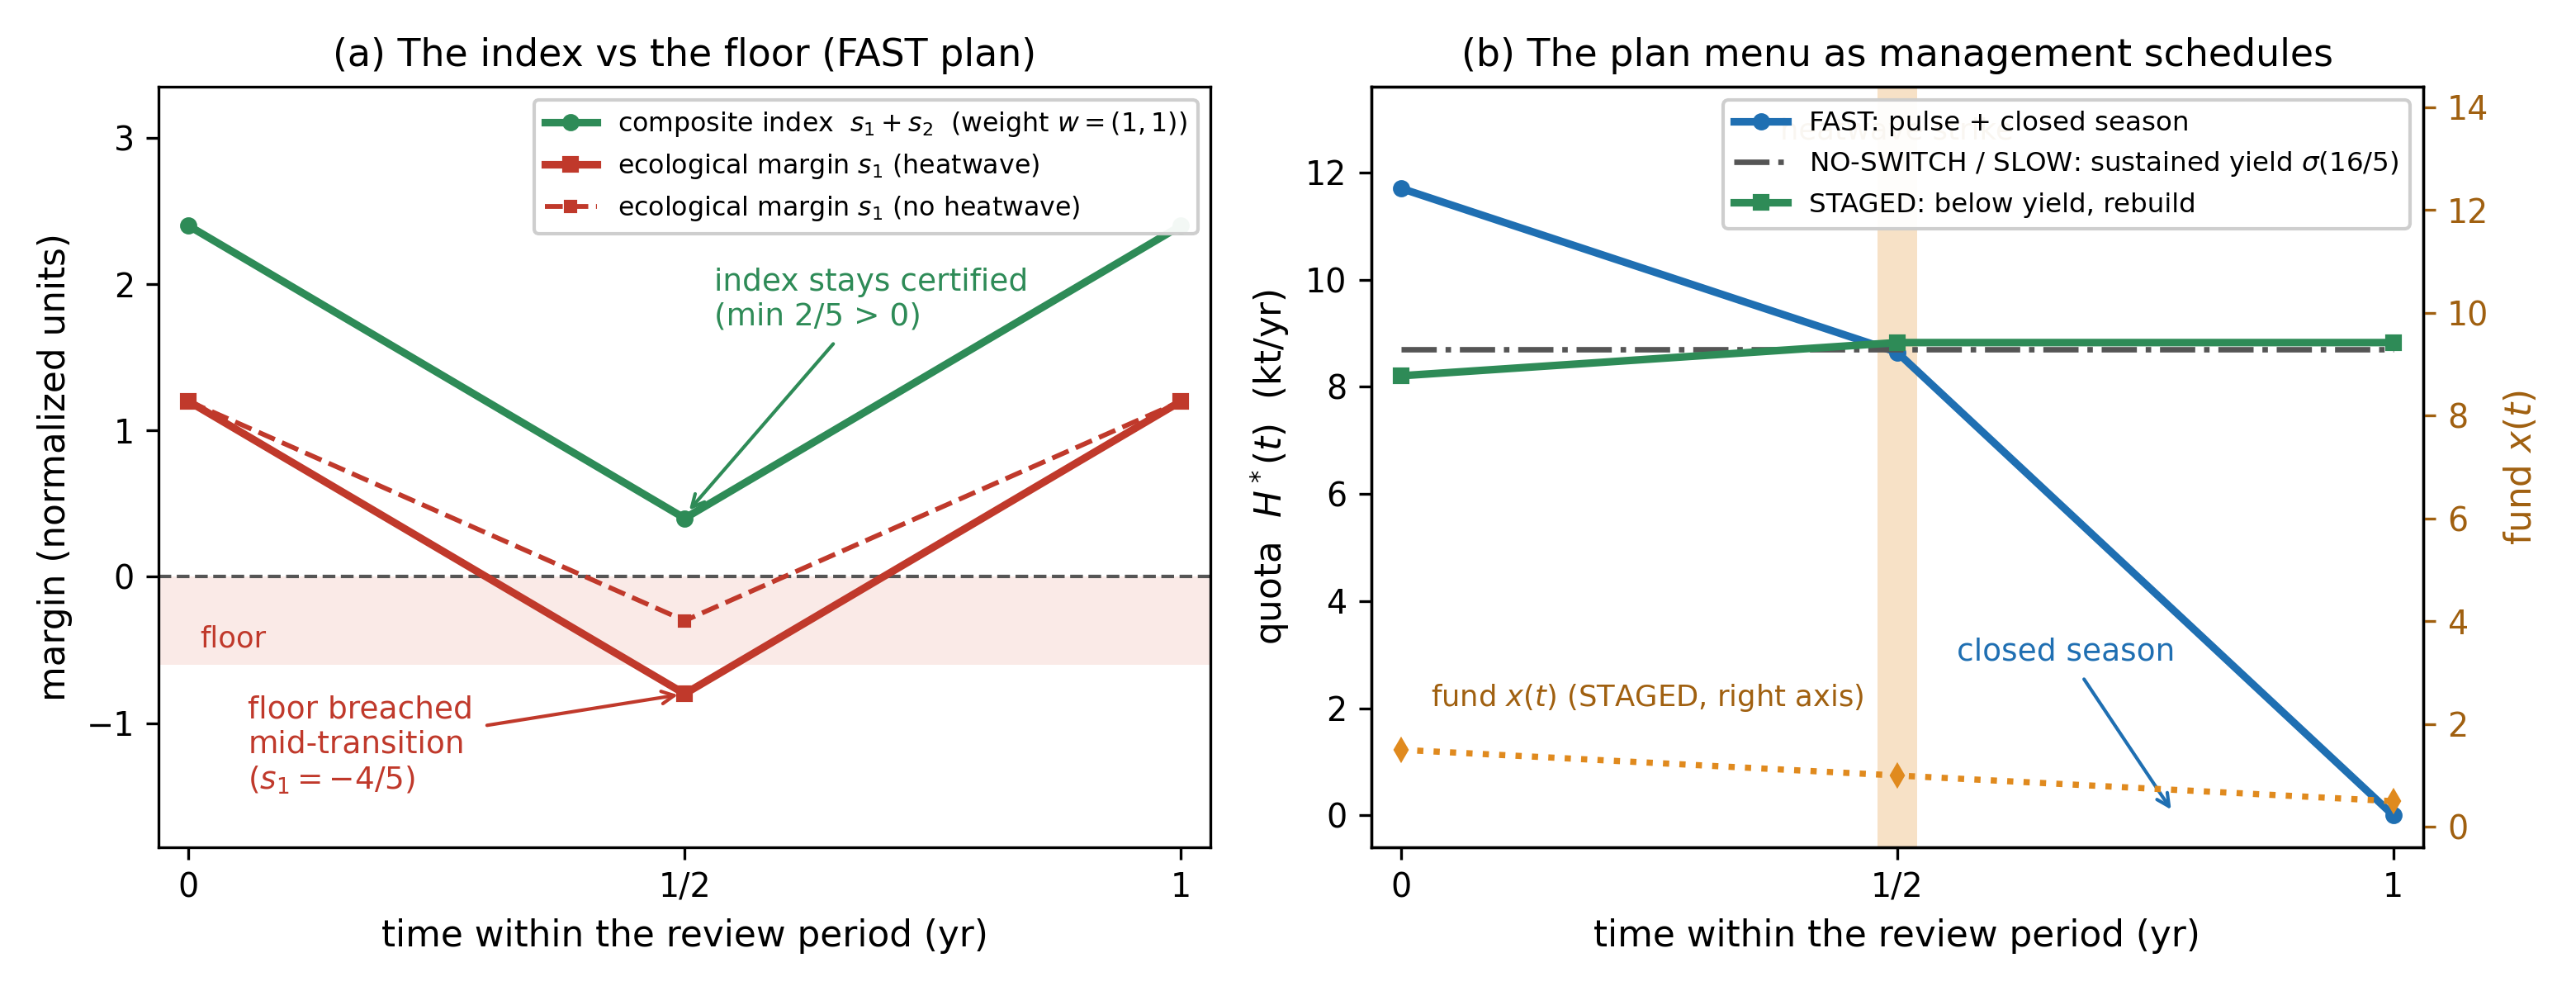
\includegraphics[width=0.98\linewidth]{figs_p1/fig_benchmark_v44.png}
\caption{The witness datum realized as a fishery-transition benchmark
(Section 6.3). (a) Under the pulse-and-closure plan, the composite index
\(s_1 + s_2\) at \(w = (1, 1)\) remains certified at every instant (minimum
\(2/5\)), while the ecological margin breaches its floor mid-transition
(\(-4/5\) under the heatwave strike, \(-3/10\) without it): the
accepted-at-every-weighting reading is blind to the breach. (b) The plan menu
as management schedules: pulse plus closed season; sustained-yield status
quo; and the reserve-financed staged transition, which rebuilds the stock
while improving both margins (the rescue set). All quota, stock, margin, and
fund values are the exact rational values verified in Section 6.3.}
\label{sep-fig:benchmark}
\end{figure}

\subsection{A resource-transition benchmark}\label{sep-resource-transition-benchmark}

The witness datum of Section 4.5 is deliberately spare: a fund, two typed
floors, four plans, and a tube semantics. This section realizes the same
datum as a standard biomass--yield resource model, so that the reader can
read every symbol as a quantity a resource agency actually monitors, and so
that the theorems can be seen to bear on a textbook dynamical system rather
than on a discrete datum alone. The instantiation is an exact rational re-reading of the witness
datum in the language of a Schaefer (1954) production model:
every number below is re-derivable from the deposited benchmark script,
which verifies it in exact rational arithmetic, and the certified tubes
are conservative for the nonlinear realization by an exact inequality. It
is not a fitted case study, and no empirical claim is made.

Read as a decision problem, the benchmark has the structure of a
certification study in multi-criteria decision aiding. The decision
maker is the resource authority; the decision alternatives are the
menu's management schedules (NO-SWITCH, FAST, SLOW, and the
reserve-financed STAGED); the criteria are the two typed floors ---
the biomass margin above the limit reference point and the fleet
income margin --- evaluated along the whole transition under the
declared disturbance; and the scalarization weights are the preference
orderings of the assessment doctrine under which the composite index
is read. The two criteria are conflicting objectives --- each of the
two principal schedules protects one at the expense of the other ---
and each is defended by a distinct constituency, so the weight space
reads both as an assessor's calibration and as the preference profile
of the stakeholder dispute. The acceptance gap is then a robustness
failure of the
decision-aiding process in the precise sense of Theorem 5: at every
preference weighting the index licenses some alternative --- possibly
a different one at different weightings --- while no single
alternative satisfies the criteria path-wise. The deliverables are
ones a decision analyst can communicate: the licensing thresholds ---
the preference ranges over which each alternative is certified --- and
the rescue threshold --- the adjustment funding that converts an
unlicensable state into a staged transition. At the asymmetric
allocations of the substitutability extension
(Section~\ref{sep-substitutability-spectrum}), the same total margin
draws opposite verdicts and opposite management responses, so the
certification boundary is operationally decision-relevant.

\textbf{The system.} Let \(B(t)\) denote spawning biomass (kt) in a
stock-specific fishery over one annual review period \(t \in [0, 1]\), with
logistic surplus production
\(\sigma(B) = r B (1 - B/K)\) at \(r = 4\), \(K = 10\), and a biomass limit
\(B_{\mathrm{lim}} = 2\) kt below which the spawning stock is judged unable
to sustain recruitment. The ecological floor is the margin
\(s_1(t) = B(t) - B_{\mathrm{lim}} \ge 0\); the income floor
\(s_2(t) \ge 0\) is the fleet income margin net of costs, maintained by the
quota and by the transition reserve \(x(t)\), an adjustment fund financing
fleet draw-down. Four plans are available, standard in transition management:
\textbf{NO-SWITCH} (status-quo harvest), \textbf{FAST} (an immediate large
quota cut --- a pulse season followed by a closure --- accepting a
mid-season trough on the ecological floor, the plan's certified
exposure), \textbf{SLOW} (a gradual reduction, shifting the burden onto
the income floor), and \textbf{STAGED} (a
below-sustained-yield quota while the reserve finances the fleet transition,
after which both margins improve). Disturbances are environmental shocks: a
mid-season heatwave strike (\(t = 1/2\)) imposing an excess mortality
\(\delta_0 = 1/2\) kt on the stock, present or absent. The state is observed
only through the institutional dashboard, the weighted aggregate
\(w \cdot (s_1, s_2)\), and the reviewer checks the dashboard, not the
floors. This is a deliberately adverse reporting architecture, adopted to
isolate the assessment-operator issue --- not a claim about current
fisheries assessment practice, in which a limit-reference-point breach
triggers a mandatory management response.

\textbf{The datum, in resource terms.} At the datum's initial state
\((x, s_1, s_2) = (1/2, 6/5, 6/5)\) --- a half-financed fund, a stock
\(B = B_{\mathrm{lim}} + 6/5 = 16/5\) kt (\(6/5\) kt \(= 1.2\) above the limit), and a
healthy income margin --- the plan menu of Section 4.5 reads: \textbf{FAST}
cuts the quota hard for half a season; with the income floor protected by its
quota schedule, FAST's exposure is the ecological floor, whose worst-case
(dip \(2\)) trajectory is \(s_1\): \(6/5 \to -4/5 \to 6/5\) --- the stock
troughs at \(B_{\mathrm{lim}} + (-4/5) = 6/5\) kt, i.e.\ \(4/5\) kt
\emph{below} the limit (\(s_1 = 6/5 - 2 = -4/5\) relative to the floor).

\textbf{SLOW} mirrors the exposure onto the income floor
(\(s_2: 6/5 \to -4/5 \to 6/5\)). \textbf{STAGED} spends the fund at the
buy-back cost \(c = 1\) while both margins improve by the destination gain
\(e = 1/4\). These are exactly the tube tables verified in Section 4.5 and
in the deposited artifact; the interpretation is new, the arithmetic is not.

\textbf{The benchmark schedule, exactly.} The FAST plan is realized by the
announced quota \(H^*(t)\) that makes the benign margin line
\(s_1\): \(6/5 \to 6/5 - 3/2 \to 6/5\) --- the tube-table line with the
heatwave's \(1/2\)-kt dip removed --- an exact trajectory
of \(\dot B = \sigma(B) - H^*(t)\): on \((0, 1/2)\),
\(H^* = 3 + \sigma(B_{\mathrm{line}}(t))\) (a pulse declining from
\(\tfrac{1463}{125} \approx 11.7\) to \(\tfrac{2161}{250} \approx 8.6\) kt/yr
--- admissible against the fleet capacity \(H_{\max} = 13\)), and on
\((1/2, 1)\) a closure, \(H^* = 0\). The benign branch then tracks the tube
line exactly. The heatwave strike at \(t = 1/2\) drops the stock by
\(\delta_0\), from the trough \(17/10\) kt to \(6/5\) kt --- the adverse
tube's value --- and the closure lets the surplus rebuild the stock: on the adverse
recovery leg the surplus is at least \(\sigma(6/5) = 528/125 > 4\) kt/yr,
while the certified recovery needs only \(4\), so the realized nonlinear
trajectory lies on or above the certified tube throughout; the certified
tubes are conservative for the Schaefer realization.

The remaining plans are
read off the same model: NO-SWITCH and SLOW hold \(B = 16/5\) at the
sustained-yield quota \(\sigma(16/5) = 1088/125 \approx 8.7\) kt/yr ---
itself below the model's maximum sustainable yield (MSY) of
\(\sigma(K/2) = rK/4 = 10\) kt/yr at \(B = K/2\); STAGED
(entered at the rescue witness, fund \(x = 3/2\)) taxes the sustained yield
by the margin improvement, rebuilding the stock
\(16/5 \to 69/20\) while the fund draws down \(3/2 \to 1/2\) and both typed
margins improve by \(e = 1/4\).

\textbf{The dashboard reading.} Under the heatwave branch of the
licensed plan, the composite index at the equal weighting, \(s_1 + s_2\),
has the tube values \((12/5, 2/5, 12/5)\): the dashboard never drops below
\(2/5\), and the transition is certified at \emph{every} weighting
(Section 4.5's per-weight thresholds \(\rho_1 = 2/3\), \(\rho_2 = 3/2\) place
FAST inside every assessor's acceptance set at income-heavy weights and SLOW
inside every assessor's at biomass-heavy weights, with their overlap
containing \(r = 1\)). The floor itself, meanwhile, is breached
mid-transition on both branches (\(-4/5\) with the strike, \(-3/10\)
without), and no plan in the menu keeps both floors path-wise --- the
aggregate dashboard certifies a transition that violates the biomass limit
on both branches --- with the strike and without it --- and no weighting
can detect this from the index alone.

The reserve threshold is the operational number: a fund below
the buy-back cost \(c = 1\) makes the staged transition
unfinanceable (\(\kappa^*(z) = 1 - x\) at the stricken states), so every
state of the failure set \(\{x < 1,\, s_1 < 2,\, s_2 < 2\}\) carries
the finite shortfall \(\kappa^* = 1 - x\); the impossibility region is
its part that the dashboard still certifies, and a modest top-up of the
adjustment fund converts it into a rescue state. In
management language: the dashboard is structurally unable to distinguish a
transition that survives the heatwave from one that does not, and the
financing gap, not the weighting, is what separates them
(Figure~\ref{sep-fig:benchmark}).

\medskip

\noindent Table~\ref{sep-tab:fisheries} completes the translation guide of
Table~\ref{sep-tab:translation} into the benchmark's own vocabulary: each of
the paper's central objects read as the fisheries quantity of this
section.

\begin{table}[htbp]
\centering
\small
\caption{The translation guide (Table~\ref{sep-tab:translation}) extended to
the fishery benchmark's own quantities.}
\label{sep-tab:fisheries}
\begin{tabular}{@{}p{4.1cm}p{9.4cm}@{}}
\toprule
Object & Fisheries reading (this section) \\
\midrule
Typed floors \(s_i \ge 0\) & the spawning-stock margin above the limit reference point (\(B - B_{\mathrm{lim}} \ge 0\); the LRP convention) and the fleet income margin net of costs \\
Scalarized operator \(E_w\) & the assessment dashboard \(w \cdot (s_1, s_2)\) the reviewer checks \\
Licensing thresholds \(\rho_1, \rho_2\) & weight-ratio licensing intervals for the pulse (FAST) and gradual (SLOW) quota plans \\
Acceptance gap \(\mathrm{FP}_{\mathrm{agg}}\) & dashboard-certified yet LRP-breaching transitions (the index-blindness zone: trough \(0.6\) LRP units while the dashboard reads \(2/5 > 0\)) \\
Rescue set \(R\); threshold \(\kappa^*\) & the adjustment fund financing fleet buy-down (STAGED at cost \(c = 1\); the shortfall \(\kappa^* = 1 - x\)) \\
Impossibility region \(I\) & underfunded transitions: fund \(x < 1\), both margins below their plan margins, dashboard still certified \\
Blend collapse vs.\ time-sharing & fractional quota/effort allocation (convexification) vs.\ pulse/gradual season alternation \\
Exact-tube semantics & no transient LRP breach along the transition, the mid-season heatwave included \\
\bottomrule
\end{tabular}
\end{table}


\textbf{A data anchor on a real stock.} The benchmark's units are not chosen in a
vacuum: they are anchored to a real, regulated floor. For Northern cod
(\emph{Gadus morhua}, NAFO Divisions 2J3KL), the assessed spawning-stock
series (NCAM M-shift, 1983--2015) carries a limit reference point (LRP) of
\(884.6\) kt (DFO, 2016) --- the biomass below which recruitment is judged
impaired; the same series underlies the companion scored test of
surplus-production forecasters on this stock (Abaee, 2026, \emph{Does a
Surplus-Production Ladder Improve Forecasts of Northern Cod?}). Reading the
benchmark's floor as this LRP fixes the dashboard arithmetic: the witness's
opening stock (\(1.6\) LRP units, \(1.6 \times 884.6 \approx 1.42\) Mt) is the
neighbourhood of the assessed mid-1980s Northern cod spawning biomass, the
adverse plan's trough (\(B = 6/5\) kt, \(0.6\) LRP units \(\approx 531\)
kt) lies below the LRP while remaining above the stock's 2015
assessed level of about a third of the LRP (\(33.8\%\), \(\approx 299\)
kt; DFO, 2016) --- the zone between the two levels, in which the stock in fact
resided after the collapse --- and the adverse plan's
worst-case stock excursion --- \(2\) kt, i.e.\ one full LRP unit (the
quota's \(3/2\)-kt draw-down plus the heatwave's \(1/2\)-kt excess
mortality) --- is the order of the stock's swing across the LRP itself.
\textbf{The motivation, with the assessed numbers.} The anchoring
statements of this subsection, made precise: the limit reference point of
the assessed NCAM M-shift series is \(884.6\) kt --- by construction the
1983--1989 mean spawning-stock biomass of that series (DFO, 2016, Table
A2); the stock's assessed 2015 level is \(33.8\%\) of that LRP (the
advisory report's ``about a third''), \(\approx 299\) kt; the decline
from the mid-1980s neighbourhood of the benchmark's opening stock
(\(\approx 1.42\) Mt) to the 2015 level is a swing of \(\approx 1.1\)
Mt, about \(1.3\) LRP units; and the benchmark's adverse worst-case
excursion --- one full LRP unit --- is therefore of the assessed order,
with its trough (\(0.6\) LRP) inside the assessed post-collapse band
\((0.34, 1)\) LRP units. The unit convention is explicit throughout:
\(s_1\) is a kt margin above \(B_{\mathrm{lim}}\), so the opening
stock is \(B(0) = B_{\mathrm{lim}} + 6/5 = 16/5\) kt, the normalized
stock is \(b(0) = B(0)/B_{\mathrm{lim}} = 8/5 = 1.6\) LRP units, and the
margin \(6/5\) kt is not itself a biomass ratio.

Three qualifications apply. The anchoring fixes units only: no
parameter of the rational witness is estimated from data, and the
theorems say nothing predictive about this or any other stock. And the companion scored test adds a caution of exactly the
discipline this paper practises: on the same series, no structural
surplus-production model in the scored ladder beat last-value persistence
(one-year RMSE \(98\) kt versus \(115\)--\(206\) kt), and every model missed
the collapse window --- what survives institutional scrutiny on such a stock
is the menu and the floors, both of which are set by management and both of
which this paper's datum takes as given, rather than a predictive fit of the
dynamics.

\begin{center}\rule{0.5\linewidth}{0.5pt}\end{center}

\section{Conclusions}\label{sep-conclusions}

Scalarized and coordinate-wise feasibility criteria are usually compared
as doctrines --- as different normative stances on substitutability, of
which the weak- and strong-sustainability traditions are the canonical
instances. This paper shows that the divergence between the two criteria
as formalized here --- the scalarized-aggregate and typed
operators of Section 3.1 on a common action menu and disturbance class
--- survives translation into assessment mechanics, at the level of a
theorem about those operators. The theorem establishes no ranking of doctrines: Section 5.1 delimits the formalizations, and by Theorem 9 the structural character of the separation is a property of the finite deterministic menu, not of either tradition (Sections 4.10--4.11). On a typed transition datum under exact-tube semantics, the
compensatory reading (per-weight acceptance) and the noncompensatory
reading (common-plan acceptance) are related by a quantifier commutation
that can fail on an open region of state space. Where it fails, every
scalarization weight certifies a transition, but no single transition is
certified by all weights, and the certified set splits into states
rescuable by a resource-controlled action and states that are impossible
under every weight. The mechanism is not scalarization blindness --- at
fixed trajectories the full-cone aggregate is lossless --- but the
policy dependence of the aggregate-feasible transition. The
finite-menu theorem of Section 4.4 states the underlying mechanism in
full generality: for any finite menu, the acceptance gap is the part of
the convex hull of the required margins that no single plan dominates,
so the witness of Section 4.5 is an instance of a geometric fact rather
than an isolated construction.

For the construction of composite sustainability indices, the theorem
has a concrete consequence. An index can be sound at the level of
accounting and still over-certify at the level of assessment, because
certification is a quantifier statement about transitions, not a
property of a number. Where separately-binding floors matter, per-floor
reporting is not a presentation preference but a detection requirement:
the aggregate alone cannot distinguish the rescue region from the
impossibility region. The bridge a composite index needs --- some single
transition that serves every admissible weight, i.e.~membership in
\(\mathcal{V}_{\mathrm{typ}}\) --- is exactly what the frameworks'
reporting conventions should be asked to exhibit. Theorem 9 qualifies this requirement: such a single transition is not, in general, a member of the specified deterministic menu but a convexified action, so the relevant question for a reporting convention is whether its action set admits the required menu convexification --- and Proposition 10 shows that temporal alternation alone does not provide it.

Read from each of the three literatures this paper connects, the results
take one specific form. For multi-criteria assessment, they locate the
certification failure of compensatory aggregates in the acceptance
protocol --- not in weight choice, and not in compensability at fixed
profiles. For decision making under uncertainty, the acceptance gap
measures the value of information about the assessment weight, and
Theorem 9 with Proposition 10 identifies menu convexification, not
temporal sharing, as what removes it. For transition management, where
separately-binding floors govern a transition, per-floor reporting along
the path is the detection requirement the separation makes exact.

\section*{List of abbreviations}\label{sep-list-of-abbreviations}

\begin{itemize}
\item \textbf{CES} --- constant elasticity of substitution
\item \textbf{DFO} --- Fisheries and Oceans Canada
\item \textbf{LPI} --- Living Planet Index
\item \textbf{LRP} --- limit reference point
\item \textbf{MSY} --- maximum sustainable yield
\item \textbf{NCAM} --- Northern Cod Assessment Model
\item \textbf{PROMETHEE} --- Preference Ranking Organisation Method for Enrichment Evaluation
\end{itemize}

\begin{center}\rule{0.5\linewidth}{0.5pt}\end{center}


\appendix

\section{Proofs of the general results}

\textbf{Proof of Remark 1 (Section 4.1).}\ If \(a \in \bigcap_\lambda E_\lambda(z)\), then each
\(E_\lambda(z)\) is nonempty, so \(z\) lies in the right-hand set. The
inclusion fails at \(z\) precisely when each \(E_\lambda(z)\) is
nonempty but \(\bigcap_\lambda E_\lambda(z) = \varnothing\), i.e.~when
no common selector exists; this is the stated equality condition. \ensuremath{\square}

\textbf{Proof of Remark 2 (Section 4.2).}\ (\(\Rightarrow\)) \(w \ge 0\), \(w \neq 0\), \(v \ge 0\)
gives \(w \cdot v = \sum_i w_i v_i \ge 0\). (\(\Leftarrow\)) If
\(v_k < 0\), take \(w = e_k \in W_+\): then \(w \cdot v = v_k < 0\). \ensuremath{\square}

\textbf{Proof of Proposition 3 (Section 4.3).}\ (i) Let \(a \in E_{\mathrm{typ}}(z)\). For every
disturbance \(d\),
\(\mathrm{Tube}(a,d) \subseteq S = S^{\mathrm{phys}} \cap \{s \ge 0\}\).
By Remark 2, every tube point satisfies \(w \cdot s \ge 0\) for every
\(w \in W_+\), and likewise every successor state lies in \(G^w\); hence
\(a \in E_w(z)\). The remaining inclusions follow from
\(S^w \subseteq S^{\mathrm{phys}}\),
\(G^w \subseteq G^{\mathrm{phys}}\), and
\(\mathrm{End}(a,d) \subseteq \mathrm{Tube}(a,d)\). (ii) The inclusion
\(\subseteq\) is part (i) intersected over \(w\). For the reverse
inclusion, let \(a \in \bigcap_{w \in W_+} E_w(z)\). For every \(d\) and
every tube point \(p \in \mathrm{Tube}(a,d)\), every \(w \in W_+\) gives
\(w \cdot s(p) \ge 0\), so by Remark 2 \(s(p) \ge 0\) componentwise;
hence \(\mathrm{Tube}(a,d) \subseteq S\). The same argument with
\(\mathrm{Succ}\) gives \(\mathrm{Succ}(a,d) \subseteq G\). Thus
\(a \in E_{\mathrm{typ}}(z)\). \ensuremath{\square}

\textbf{Proof of Proposition 4 (Section 4.4).}\ For the second inclusion: by Proposition 3(i),
\(E_w(z) \subseteq E_{\mathrm{tube,phys}}(z)\) for every \(w\), so
\(\mathcal{V}_w \subseteq \mathcal{V}_{\mathrm{phys}}\), and
intersecting over \(w \in W\) preserves the inclusion. For the first: if
\(z \in \mathcal{V}_{\mathrm{typ}}\), then by Proposition 3(ii) there
exists \(a \in \bigcap_{w \in W_+} E_w(z)\); this same \(a\) lies in
\(\bigcap_{w \in W} E_w(z)\), so \(E_w(z) \neq \varnothing\) for every
\(w \in W\), i.e.~\(z \in \mathcal{V}_W\). Monotonicity: intersecting
over a larger family can only shrink the intersection. \ensuremath{\square}

\textbf{Proof of the finite-menu theorem (Section 4.4).}\ (i) is the margin test restated. For (ii), if
\(s = d + v\) with \(d \in \operatorname{conv}(\mathcal{D})\) and \(v \ge 0\), then
for every \(w \ge 0\), \(w \cdot s \ge w \cdot d \ge \min_a w \cdot d_a\),
so the scalarized test holds. Conversely, suppose
\(s \notin \operatorname{conv}(\mathcal{D}) + \mathbb{R}^n_+\); this set is closed
and convex (a compact polytope plus a closed cone), so strict separation
gives \(w \ne 0\) with \(w \cdot s < w \cdot d + w \cdot v\) for every
\(d \in \operatorname{conv}(\mathcal{D})\) and every \(v \ge 0\). Since \(v\)
ranges over the whole cone, \(w \in \mathbb{R}^n_+ \setminus \{0\}\), and
taking \(v = 0\) gives
\(w \cdot s < \min_{d \in \operatorname{conv}(\mathcal{D})} w \cdot d =
\min_a w \cdot d_a\): the scalarized test fails. \ensuremath{\square}

\section{Proofs for the witness datum}

\textbf{Proof of Theorem 5 (Section 4.6).}\ \textbf{(1)} Typed admissibility requires the worst-case
tube in \(S_0\) and the successor in \(G\). NO-SWITCH never reaches
\(G\) (its successor retains \(q = 0\)), so it is never admissible. For
FAST, the worst-case \(s_1\)-tube is \([s_1 - 2, s_1]\), safe if and
only if \(s_1 \ge 2\); its successor \((1, x, s + e)\) lies in \(G\)
given \(x \ge 0\). Hence FAST is typed-admissible exactly when
\(s_1 \ge 2\). Symmetrically, SLOW is typed-admissible exactly when
\(s_2 \ge 2\). For STAGED, the floors grow through the interval and the
successor lies in \(G\); the binding constraint is the \(x\)-tube
\([x - 1, x]\), safe if and only if \(x \ge 1\). Therefore
\(E_{\mathrm{typ}}(z) \neq \varnothing\) exactly on
\(\{x \ge 1\} \cup \{s_1 \ge 2\} \cup \{s_2 \ge 2\}\).

\textbf{(2)} Fix \(w = (w_1, w_2) \in W_+\). NO-SWITCH misses \(G^w\)
and is never admissible. FAST is \(w\)-admissible if and only if its
worst-case aggregate value stays nonnegative:
\(w_1(s_1 - 2) + w_2 s_2 \ge 0\), i.e.~\(w_1 s_1 + w_2 s_2 \ge 2 w_1\)
(automatic when \(w_1 = 0\)). Symmetrically SLOW is \(w\)-admissible if
and only if \(w_1 s_1 + w_2 s_2 \ge 2 w_2\). STAGED is \(w\)-admissible
if and only if \(x \ge 1\) (the physical constraint within \(S^w\)),
since \(w \cdot s \ge 0\) holds automatically along its tube. Hence
\(z \in \mathcal{V}_w\) whenever \(x \ge 1\); and if \(x < 1\), then
\(z \in \mathcal{V}_w\) if and only if at least one of the two
inequalities above holds.

Suppose first \(x \ge 1\): then \(z \in \mathcal{V}_w\) for every \(w\),
so \(z \in \mathcal{V}_{\mathrm{weak}}\). Suppose \(x < 1\) and
\(s_1 \ge 2\) or \(s_2 \ge 2\): say \(s_1 \ge 2\); then FAST is
typed-admissible by (1), hence \(w\)-admissible for every \(w\), so
\(z \in \mathcal{V}_{\mathrm{weak}}\). It remains to treat \(x < 1\)
with \(s_1 < 2\) and \(s_2 < 2\). For \(w_1 > 0\), write
\(r = w_2/w_1\): FAST is \(w\)-admissible exactly when
\(s_1 + r s_2 \ge 2\), i.e.~\(r \ge (2 - s_1)/s_2 = \rho_1\) (using
\(s_2 > 0\); when \(s_2 = 0\) the condition reduces to \(s_1 \ge 2\),
which is excluded). SLOW is \(w\)-admissible exactly when
\(s_1 + r s_2 \ge 2r\), i.e.~\(r \le s_1/(2 - s_2) = \rho_2\) (using
\(s_2 < 2\)). The boundary weights are the same limiting cases: at
\(w_1 = 0\) (\(r \to \infty\)) FAST is licensed provided \(s_2 \ge 0\),
while SLOW is strictly rejected on the region \(s_2 < 2\);
symmetrically, at \(w_2 = 0\) (\(r = 0\)) SLOW is licensed provided
\(s_1 \ge 0\), while FAST is rejected on the region \(s_1 < 2\).
Therefore \(z \in \mathcal{V}_w\) for every \(w \in W_+\) if and only if
the intervals \(\{r \ge \rho_1\}\) and \(\{r \le \rho_2\}\) together
cover all of \([0, \infty]\), which holds exactly when
\(\rho_2 \ge \rho_1\). Computing,
\[\rho_2 \ge \rho_1 \iff \frac{s_1}{2 - s_2} \ge \frac{2 - s_1}{s_2} \iff s_1 s_2 \ge (2 - s_1)(2 - s_2) \iff s_1 + s_2 \ge 2,\]
with both denominators positive in the present case. Hence, in this
case, \(z \in \mathcal{V}_{\mathrm{weak}}\) if and only if
\(s_1 + s_2 \ge 2\). Assembling the three cases, and noting
\(\{s_1 \ge 2\} \cup \{s_2 \ge 2\} \subseteq \{s_1 + s_2 \ge 2\}\) under
nonnegativity,
\[\mathcal{V}_{\mathrm{weak}} = \{ x \ge 1 \} \cup \{ s_1 + s_2 \ge 2 \}.\]

\textbf{(3)} In the physical operators the only constraint is
\(x \ge 0\) (with \(q = 1\) at the destination). FAST and SLOW have
tubes within \(S^{\mathrm{phys}}\) and successors in
\(G^{\mathrm{phys}}\) for every \(z \in X_0\) (their dips affect only
\(s\), which is unconstrained physically); STAGED does so exactly for
\(x \ge 1\). Hence \(E_{\mathrm{tube,phys}}(z) \neq \varnothing\) for
every \(z \in X_0\), so \(\mathcal{V}_{\mathrm{phys}} = X_0\). For the
endpoint operator, the endpoint values of FAST and SLOW lie in
\(S^{\mathrm{phys}}\) for every \(z \in X_0\), so
\(\mathcal{V}_{\mathrm{end}} = X_0\) as well.

\textbf{(4)} By (1)--(2),
\[\mathrm{FP}_{\mathrm{agg}} = \mathcal{V}_{\mathrm{weak}} \setminus \mathcal{V}_{\mathrm{typ}}
= \big[ \{x \ge 1\} \cup \{s_1 + s_2 \ge 2\} \big] \setminus \big[ \{x \ge 1\} \cup \{s_1 \ge 2\} \cup \{s_2 \ge 2\} \big]\]
\[= \{ x < 1,\ s_1 < 2,\ s_2 < 2,\ s_1 + s_2 \ge 2 \} = I.\]
This set is nonempty
(e.g.~\((x, s_1, s_2) = (\tfrac12, \tfrac65, \tfrac65)\)), and its
relatively open interior is the stated region.

\textbf{(5)} By (4),
\(I = \mathrm{FP}_{\mathrm{agg}} = \mathcal{V}_{\mathrm{weak}} \setminus \mathcal{V}_{\mathrm{typ}} \neq \varnothing\),
so the first inclusion is strict. For the second, the point
\((\tfrac12, \tfrac1{10}, \tfrac1{10})\) satisfies \(x < 1\) and
\(s_1 + s_2 = \tfrac15 < 2\), so it lies outside
\(\mathcal{V}_{\mathrm{weak}}\) by (2), while by (3) it lies in
\(\mathcal{V}_{\mathrm{phys}}\).

\textbf{(6)} The threshold characterization was derived in the proof of
(2): with \(r = w_2 / w_1\), FAST is licensed exactly for
\(r \ge \rho_1\) and SLOW exactly for \(r \le \rho_2\), and
\(\rho_2 \ge \rho_1 \iff s_1 + s_2 \ge 2\). On \(\mathcal{Q}\) the
inequality \(s_1 + s_2 \ge 2\) holds, so the two licensing intervals
overlap and together cover all weights; strictly on the relative
interior (\(s_1 + s_2 > 2\)) both thresholds are finite and the
intervals overlap in a nondegenerate interval, with \(r > \rho_2\)
licensing FAST only and \(r < \rho_1\) licensing SLOW only. On \(I\)
(where \(x < 1\)), STAGED is inadmissible for every \(w\), so
\(E_{\mathrm{typ}}(z) = \bigcap_w E_w(z) = \varnothing\) by Proposition
3(ii): no single action serves every weight. On \(R\) (where
\(x \ge 1\)), STAGED lies in \(E_{\mathrm{typ}}(z) = \bigcap_w E_w(z)\)
and serves every weight.

\textbf{(7)} On \(R\), STAGED's tube is
\([x - 1, x] \times \{s \to s + e\}\): the \(x\)-tube stays nonnegative
because \(x \ge 1\), the floors grow, and the successor
\((1, x - 1, s + e) \in G\). On \(I\), the four exhibited violations
exhaust the action set and each violates a typed constraint: FAST's
\(s_1\)-tube reaches \(s_1 - 2 < 0\); SLOW's \(s_2\)-tube reaches
\(s_2 - 2 < 0\); STAGED's \(x\)-tube reaches \(x - 1 < 0\); NO-SWITCH's
successor misses \(G\). \ensuremath{\square}

\textbf{Proof of Remark 7 (Section 4.8).}\ (i) Backward induction on stages. Base: at the final stage
the terminal sets satisfy
\(G \subseteq G^w \subseteq G^{\mathrm{phys}}\) by Remark 2 and the
definition of the terminal sets. Step: the accepted set of a stage is
the set of states from which some action keeps the tube in the safe set
and the successor in the next-stage accepted set; applying Proposition
3(i) to the stage's action sets and the induction hypothesis to the
next-stage accepted sets preserves the three-way inclusion at the stage
level. (ii) With HOLD the unique prefix action, a prefix state is
accepted exactly when it lies in the prefix safe set and in the
next-stage accepted set; the stage-0 regions are therefore the witness
regions of Theorem 5 pulled back through the (identity) holds, and the
strictness witnesses (\(I \neq \varnothing\) and the point
\((\tfrac12, \tfrac1{10}, \tfrac1{10})\)) persist. (iii) The three
listed mechanisms are each sufficient to erase the gap in a multi-stage
setting, so no unconditional generalization is asserted. \ensuremath{\square}

\textbf{Proof of Theorem 8 (Section 4.8).}\ \emph{Datum.} Two capital forms, floors at zero, the bridge stock absent
(\(x \equiv 0\)); states are pairs \(s = (s_1, s_2)\). Stage 2 (final
interval): safe set \(S_0^{(2)} = \mathbb{R}^2\) (no path constraint),
terminal sets \(G^{(2)} = G^{w,(2)} = G = \{ s \ge 0 \}\) --- coincident
for every weight --- and a single action REPAIR with tube \(\{s\}\)
(safe trivially) and successor \((1, 1) \in G\). Stage 1: safe set
\(S_0 = \{ s \ge 0 \}\); two actions with constant tubes, safe at every
state of \(S_0\): A1 with successor \((s_1 - 1, s_2 + 1)\) and A2 with
successor \((s_1 + 1, s_2 - 1)\); the stage-1 terminal architecture is
the stage-2 accepted sets. Initial state \(z^* = (\tfrac25, \tfrac25)\).

\emph{In the two-stage datum the gap is erased.} REPAIR is
typed-admissible --- hence \(w\)-admissible for every weight --- from
every state, so
\(\mathcal{V}_{\mathrm{typ}}^{(2)} = \mathcal{V}_w^{(2)} = \mathbb{R}^2\)
for every \(w\): the stage-2 accepted sets coincide. Backward induction
then admits both A1 and A2 at \(z^*\) (safe tubes; successors in
\(\mathcal{V}_{\mathrm{typ}}^{(2)} = \mathbb{R}^2\)), so \(z^*\) is
typed-accepted at stage 0, and weak acceptance follows from typed
acceptance.

\emph{In the single-interval truncation --- the same stage-1 datum with
the final interval collapsed to its terminal sets, \(G = \{s \ge 0\}\)
and \(G^w = \{w \cdot s \ge 0\}\) --- the gap is present.} Both
successors leave \(G\) (\(s_1 - 1 = -\tfrac35 < 0\) and
\(s_2 - 1 = -\tfrac35 < 0\)), so \(z^*\) is typed-rejected. For the weak
doctrine, writing \(r = w_2 / w_1\) on the interior of the weight cone:
A1 is \(w\)-admissible exactly when \((s_1 - 1) + r (s_2 + 1) \ge 0\),
i.e.~\(r \ge \tfrac{1 - s_1}{s_2 + 1} = \tfrac37\); A2 exactly when
\((s_1 + 1) + r (s_2 - 1) \ge 0\),
i.e.~\(r \le \tfrac{s_1 + 1}{1 - s_2} = \tfrac73\); the two intervals
cover \([0, \infty]\) because \(\tfrac37 < \tfrac73\), and the boundary
weights are covered directly (\(r = 0\): A2 gives
\(w_1(s_1 + 1) \ge 0\); \(r \to \infty\): A1 gives
\(w_2(s_2 + 1) \ge 0\)). Hence \(z^* \in \mathcal{V}_{\mathrm{weak}}\)
in the truncation, and the gap
\(\mathcal{V}_{\mathrm{weak}} \setminus \mathcal{V}_{\mathrm{typ}}\)
contains \(z^*\). \ensuremath{\square}

\textbf{Proof of Theorem 9 (Section 4.10).}\ (i) FAST's worst-case tube has \(s_1\)-coordinates
\([s_1 - 2, s_1]\) and \(s_2\)-coordinate \(\{s_2\}\); SLOW's has
\(s_1\)-coordinate \(\{s_1\}\) and \(s_2\)-coordinates
\([s_2 - 2, s_2]\); both keep \(x\) nonnegative throughout (their dips
affect only \(s\)). The blended tube therefore has \(s_1\)-coordinates
\([s_1 - 2\delta, s_1]\), \(s_2\)-coordinates
\([s_2 - 2(1-\delta), s_2]\), and nonnegative \(x\)-coordinates (convex
combinations of nonnegative quantities). Typed admissibility requires
the tube within \(S_0 = \{x \ge 0, s \ge 0\}\) and the successor in
\(G\). The tube condition is exactly the displayed window. The successor
is the mixture of the two successors, which the datum fixes to the same
value --- the action table of Section 4.5 gives both FAST and SLOW the
successor \((1, x, s + e)\) --- so the blended successor is
\((1, x, s + e) \in G\): \(x \ge 0\) and the destination label is \(1\).
The window is nonempty exactly when \(1 - s_2/2 \le s_1/2\),
i.e.~\(s_1 + s_2 \ge 2\); on \(\mathcal{Q}\) the raw window already
lies in \((0,1)\) (\(s_1 < 2, s_2 < 2\) give \(0 < 1 - s_2/2\) and
\(s_1/2 < 1\)), so the \([0,1]\) clip in the statement is inactive
there; at equality it is the singleton
\(\delta = s_1/2 = 1 - s_2/2\), feasible because \(S_0\) is closed. On
the boundary faces (\(s_1 = 0\) or \(s_2 = 0\)) the window is closed at
the corresponding endpoint, and the classification follows the boundary
conventions of Section 4.6.

\begin{enumerate}
\def\labelenumi{(\roman{enumi})}
\setcounter{enumi}{1}
\item
  If \(s_1 + s_2 \ge 2\), (i) supplies a typed-admissible blend whatever
  the value of \(x \ge 0\); if \(s_1 + s_2 < 2\), no blend is
  typed-admissible by (i), and the deterministic menu contributes
  exactly
  \(\mathcal{V}_{\mathrm{typ}} = \{x \ge 1\} \cup \{s_1 \ge 2\} \cup \{s_2 \ge 2\} \subseteq \{x \ge 1\} \cup \{s_1 + s_2 \ge 2\}\).
  Hence the augmented typed set equals
  \(\{x \ge 1\} \cup \{s_1 + s_2 \ge 2\} = \mathcal{V}_{\mathrm{weak}}\)
  by Theorem 5(2) --- and nothing beyond, since every admissible blend
  satisfies \(s_1 + s_2 \ge 2\) and the deterministic actions stay
  within \(\mathcal{V}_{\mathrm{typ}}\).
\item
  Immediate from the window's state dependence and from typed
  admissibility implying \(w\)-admissibility for every weight.
\end{enumerate}

\ensuremath{\square}

\textbf{Proof of Proposition 10 (Section 4.11).}\ A sequential policy that spends any positive time on FAST
visits every \(s_1\) in \([s_1 - 2, s_1]\) and any positive time on SLOW
visits every \(s_2\) in \([s_2 - 2, s_2]\); the union tube stays within
\(S_0 = \{x \ge 0, s \ge 0\}\) exactly when both dips are nonnegative,
i.e.~\(s_1 \ge 2\) and \(s_2 \ge 2\). On \(I\) both coordinates are
strictly below 2, so the union tube is never within \(S_0\) and no
sequential policy is typed-admissible; since every member of the finite
deterministic menu is typed-admissible on \(I\) only in the per-weight
sense of Theorem 5(6) (and never in the common sense), the
noncompensatory accepted set does not extend to \(I\) under sequential
time-sharing. \ensuremath{\square}

\section{Proof of the rescue threshold}

\textbf{Proof of the rescue threshold (Section 5.7).}\ Among the augmented menu, only \(\mathrm{STAGED}_\kappa\) depends on \(\kappa\), and its typed-admissibility is independent of the floors: its \(x\)-tube is \([x + \kappa - 1,\; x + \kappa]\), the floors are nondecreasing (they grow to \(s + e\) with \(e = (\tfrac14, \tfrac14) > 0\)), and the successor \((1, x + \kappa - 1, s + e)\) lies in \(G\) exactly when \(x + \kappa - 1 \ge 0\). Hence \(\mathrm{STAGED}_\kappa \in E_{\mathrm{typ}}(z) \iff x + \kappa \ge 1\), for every \(z\). If \(z \in \mathcal{V}_{\mathrm{typ}}\), some base action of \(\mathcal{A} \subseteq \mathcal{A}_\kappa\) is admissible at \(\kappa = 0\), so \(\kappa^*(z) = 0\). If \(z \notin \mathcal{V}_{\mathrm{typ}}\) --- that is, \(x < 1\) and \(s_1 < 2\) and \(s_2 < 2\) --- then NO-SWITCH, FAST, and SLOW all fail (Theorem 5(1)), the only admissible element of \(\mathcal{A}_\kappa\) is \(\mathrm{STAGED}_\kappa\), and it is admissible exactly for \(\kappa \ge 1 - x\); hence \(\kappa^*(z) = 1 - x\). \ensuremath{\square}

\part*{Part II --- The typed ledger: what a lawful aggregate would have to be}
\label{part:ledger}
\addcontentsline{toc}{part}{Part II --- The typed ledger}

\maketitle

\section*{Abstract}\label{led-abstract}

Depletion indicators can carry similar units while built to inform distinct questions. Reserve-life ratios, trend-persistence metrics, and gross-removal pressure scales are widely interpreted as a literal ``time to depletion,'' despite measuring distinct physical or statistical quantities. Compounding this ambiguity, compensatory scalar aggregation routinely masks critical physical deficits behind positive aggregates.

In this paper, we resolve these confusions by constructing a typed stock--flow accounting ledger. By tracking conserved substance classes (\emph{moieties}) independently, conservation laws remain strictly typed: biomass, financial flows, and biodiversity metrics cannot be summed into a single scalar. Mass conservation follows directly from the incidence structure of the compartment--flux network, nonnegativity is guaranteed by donor limitation (primitive outflows vanish whenever their source compartment empties), and ecosystem services are treated strictly as observable readouts rather than conserved mass.

We formalize three certification layers: a flux-reconstruction identity that recovers unobserved internal fluxes from observed stock trajectories, a conservation-law reduction, and an envelope theorem providing verifiable flux-bounding certificates. For the closed finite-donor ledger, we establish the natural-block mass identity, orthant invariance, the absence of interior rest points under positive extraction effort, a characterization of the vanishing-extraction rest set (extinction, carrying capacity, and a frozen-biomass face), and extraction integrability over finite budgets. Furthermore, we unpack ``depletion time'' into three mutually non-interchangeable concepts: gross turnover intensity, a frozen-rate local ratio, and a scenario-conditioned hitting time equipped with uniform-drift bounds.

We classify three widely cited public-data indicators within this taxonomy: the G3P groundwater anomaly index is shown to be a record-relative statistical metric rather than a physical stock ratio; the USGS phosphate reserve-life ratio is an arithmetic convention of an economic class rather than an exhaustion forecast; and fisheries removals-only timescales represent gross pressure scales rather than demographic depletion diagnostics. We prove that no nonnegative linear weighting can universally certify componentwise nonnegativity on arbitrary balance domains, and we establish five double-counting rules to prevent the emergence of phantom mass. Finally, we formulate first-passage semantics on declared stochastic surrogates against record-relative barriers alongside explicit non-claims. Weak and strong sustainability emerge not as competing paradigms, but as two operational regimes of a single dynamic system, governed by whether material cycles close at the rate of throughput.

\textbf{Keywords:} material flow accounting, stock--flow ledger, depletion indicators, first-passage time, conservation laws, composite indicators, reserve life.

\section*{1. Introduction}\label{led-introduction}

\subsection*{1.1 Failure Modes and the Two Confusions}\label{led-11-failure-modes-and-the-two-confusions}

Sustainability accounting consistently suffers from two structural pathologies:

\begin{enumerate}\setlength{\itemsep}{2pt}
\item \textbf{Compensatory Aggregation:} Heterogeneous physical stocks and service flows are compressed into scalar indices. Because cross-component substitution rates are rarely declared formally, acute physical deficits in one critical sub-system are mathematically obscured by surpluses elsewhere. While the composite-indicator and ecological economics literatures have long critiqued this flaw and proposed noncompensatory remedies (Munda \& Nardo, 2009; Ekins et al., 2003; Neumayer, 2013), scalar index construction remains ubiquitous.
\item \textbf{Classification Drift:} Heterogeneous metrics with the dimension of time---reserve-life ratios, trend-persistence indicators, and removals-only pressure scales---are conflated into a single catch-all quantity: ``time to depletion.'' Yet, these metrics answer fundamentally different questions under incompatible boundary assumptions.
\end{enumerate}

The operational reality of classification drift is striking. A reserve-life ratio simply divides an economically declared reserve by current annual production, christening the quotient a ``depletion horizon.'' A satellite groundwater anomaly index fits a linear trend to gravimetric anomalies, reporting the time needed to reach the historical record minimum at current rates; the result is expressed in years, yet corresponds to no physical exhaustion event. A fisheries pressure scale scales a logarithmic biomass margin by instantaneous fishing mortality, presenting a gross clearance timescale as if it were a demographic extinction date. Each metric provides specific institutional or descriptive information; none represents what is popularly claimed.

The primary manifestation of compensatory aggregation is exemplified by public awareness metrics such as \emph{Earth Overshoot Day}. By collapsing ecological footprints and biocapacities into a single annual calendar date, a catastrophic deficit in an irreplaceable sub-component can easily coexist with an aggregate overshoot date that falls comfortably late in the calendar year (Lin et al., 2018; Wackernagel \& Beyers, 2019; Blomqvist et al., 2013). Systems-dynamics models encounter identical aggregation ambiguities when multidimensional state spaces are collapsed into scalar stress variables (Meadows et al., 1972). The framework developed here is component-resolved by construction: depletion horizons are defined and tracked per asset and per pool, completely precluding cross-component summation into a scalar date.

Beyond these accounting failures lies a deeper dynamical failure mode: the \textbf{productivity illusion}. This is the deceptive phenomenon in which an extractive system appears fully functional while the underlying support base sustaining its throughput is liquidated silently.

It has two senses, and they are distinct. The first is arithmetic and is the compensatory-aggregation failure above --- a deficit in one component offset by a surplus in another, so that a positive aggregate reads as adequate. This article formalises this sense as the aggregation obstruction of Section 10.1. The second sense is dynamical and is yield inflation. A measured yield can exceed the true sustainable yield when it is maintained by drawing down the support pool --- groundwater, soil carbon, bioavailable nutrients --- rather than by that pool's regeneration. The resource appears productive while what sustains it is liquidated silently.

\begin{itemize}\setlength{\itemsep}{2pt}
\item This is simply compensatory aggregation in disguise---a deficit in an unmonitored capital stock is mathematically masked by current consumption flows. We formalize this limitation as an aggregation obstruction in Section 10.1.
\item Here, harvest or extraction yield remains high because the system draws down an unmodeled support pool---such as fossil groundwater, soil organic matter, or parent mineral deposits---rather than operating within the regenerative flux of that pool. The resource appears highly productive precisely because its natural foundation is being liquidated.
\end{itemize}

The support pool need not be an absolute, non-renewable geological stock. Whether framed as natural capital, an abiotic storage compartment, or a slowly replenishing ecosystem service, the governing physics remains identical. Every such pool regenerates over some characteristic timescale: an agricultural crop regenerates seasonally, an alluvial aquifer over decades or centuries, and mineral deposits over geological epochs.

The viability of the system depends strictly on the rate of extraction relative to the rate of regeneration:

\[ \text{Extraction sustained by regeneration} \implies \text{Sustainable Throughput} \]

\[ \text{Extraction exceeding regeneration} \implies \text{Stock Liquidation} \]

A drawdown is recoverable if and only if the rate of harvest drops below the rate of replenishment before structural collapse occurs. The physical size of a reserve determines its absolute capacity; whether an ongoing extraction pattern represents sustainable harvest or irreversible liquidation depends entirely on the flow rates.

Dynamically, yield inflation mimics an overloaded mechanical structure. An elevator engineered for ten passengers can readily hold fourteen: the cable does not snap immediately upon loading the fourteenth person. Rather, it accumulates unseen microscopic strain. To the passengers, the ride feels normal until the threshold of tensile failure is breached, at which point catastrophe is instantaneous. Yield inflation corresponds to this silent wear phase: observable extraction rates remain stable, giving no hint of the drawdown occurring beneath the surface.

Our two-pool architecture is engineered specifically to capture this wear phase---making resource liquidation measurable while the supporting structure is still functional, rather than attempting to forecast the precise moment of failure.

Classification drift on the empirical side is equally well-documented. A reserve-life ratio (\(\text{Reserves}/\text{Production}\)) is purely arithmetic. Because an economic ``reserve'' is defined by extraction technology, market prices, exploration budgets, and legal permissions, it does not represent an immutable physical inventory. It replenishes dynamically through new discoveries and shifting economics. This issue has been demonstrated for phosphate rock by Illakwahhi, Vegi, and Srivastava (2024), who showed that widely publicized claims of global phosphorus exhaustion within a century stem from an uncritical reading of single-source U.S. Geological Survey (USGS) data. Such projections disregard industrial recycling, price feedbacks, and technological substitution. In mineral economics, this distinction between reserves (economic inventories) and resources (crustal abundance) has been recognized since Tilton (2003). For example, United States phosphate reserves have remained stable near \(1.0\times 10^6\text{ kt}\) for decades despite cumulative extraction exceeding \(6.0\times 10^5\text{ kt}\) over the same period. Copper demonstrates an identical dynamic: global reserves have increased over a century of exponential extraction (Tilton \& Lagos, 2007).

Similar ambiguities plague material flow accounting (MFA; Brunner \& Rechberger, 2004; Eurostat, 2001; Fischer-Kowalski et al., 2011). While MFA shares its incidence structure with chemical reaction network theory (Feinberg, 2019), practitioners frequently conflate four distinct operational properties:

\begin{enumerate}\setlength{\itemsep}{2pt}
\item \textbf{Bookkeeping balance} (mass accounting),
\item \textbf{Stoichiometric conservation} (reaction invariants),
\item \textbf{Thermodynamic admissibility} (nonnegative entropy production),
\item \textbf{Barrier safety} (maintenance of state variables within viability sets).
\end{enumerate}

A perfectly balanced mass ledger can be chemically absurd; a chemically consistent network may violate all declared ecological safety barriers; and a trajectory satisfying every environmental constraint may violate basic conservation laws through phantom mass injections. Disentangling these layers and establishing their formal relations is the first primary objective of this work (Section 3).

Our second objective is to enforce \textbf{noncompensation}. Ecological economics asserts the \emph{weak comparability of values}, maintaining that multi-criteria environmental decisions cannot be collapsed into a single metric without arbitrary value judgments (Martinez-Alier, Munda, \& O'Neill, 1998). At the level of physical accounting, this thesis takes an exact algebraic form (Section 10.1): \emph{no nonnegative linear weighting of balance vectors can certify that every underlying physical stock remains above its minimum critical threshold}. A positive weighted sum can never prove componentwise nonnegativity. Scalar indices are suitable for high-level communication and rough ranking; physical certification requires evaluating the full vector.

Our third objective is to integrate \textbf{technological substitution} directly into the ledger's internal architecture, rather than treating it as an exogenous correction. We formalize weak and strong sustainability not as irreconcilable ethical doctrines, but as two distinct operating regimes of a single dynamic system:

\begin{itemize}\setlength{\itemsep}{2pt}
\item \textbf{Weak Sustainability Regime:} Extractive throughput and population demands are small enough relative to technological substitution and natural biogeochemical cycling that material loops can close at the rate of extraction. The dominant stabilizing term over human horizons is technical substitution, with deep-time geological regeneration treated as a slow boundary condition (Daly, 1990). In this regime, metabolic byproducts---atmospheric carbon, agricultural runoff, mineral processing tailings---are returned to productive reuse fast enough that they never accumulate as unmanageable sinks. Here, ``waste'' is not an inherent property of a material, but an operational condition: matter that currently cannot be reused due to constraints in technology, economics, or logistical capacity.
\item \textbf{Strong Sustainability Regime:} The material loop fails to close at the required throughput rate, either because no physical recycling pathway exists or because industrial extraction outpaces technological implementation (Neumayer, 2013; Ekins et al., 2003). In this regime, substitution is physically admissible only when explicit stoichiometric mechanisms route matter through viable regenerative channels without depleting adjacent critical stocks. Substitution cannot be assumed via smooth Cobb--Douglas production elasticity; it requires physical mass pathways.
\end{itemize}

These two regimes reflect two distinct mathematical views of the same ledger:

\begin{itemize}\setlength{\itemsep}{2pt}
\item \textbf{The Aggregate Scalar View (\(B = b \cdot M\)):} Here, \(b\) is the specific replenishment rate and \(M\) is total natural mass. This view evaluates whether the system balances in aggregate---the central criterion of weak sustainability.
\item \textbf{The Componentwise Vector View:} This perspective assesses whether closing one balance requires the catastrophic liquidation of an unmonitored donor compartment or the overfilling of a waste sink.
\end{itemize}

Both views are indispensable. The componentwise ledger maintains stocks as first-class physical entities and tracks the hitting times and sink boundaries that constrain the aggregate throughput \(B\). The scalar check provides an instantaneous operational measure of overshoot. However, both are strictly instantaneous tests; neither can guarantee that a balanced state will persist without drifting into overshoot over time.

To quantify this drift, we construct scenario-conditioned hitting times (Section 6.5.2). When applied to economic reserves, these hitting times capture the institutional assumptions embedded within reserve classifications, converting static ratios into rigorous diagnostics.

\subsection*{1.2 Contributions}\label{led-12-contributions}

\begin{itemize}\setlength{\itemsep}{2pt}
\item \textbf{A Typed Primitive-Flux Ledger:} We formalize physical compartments by assigning each a material identity, spatial boundary, and physical unit. Compartments are linked via a signed incidence matrix driven by nonnegative primitive fluxes, synthesizing the accounting discipline of MFA (Brunner \& Rechberger, 2004) with the algebraic formalism of reaction network theory (Feinberg, 2019). Type conversions require explicit stoichiometric coefficients, and all unilateral mass transfers are strictly donor-limited.
\item \textbf{Separation of Three Certification Layers:} We mathematically separate and prove the relationships between:
\item \emph{Accounting consistency} (local preservation of balance equations),
\item \emph{Conservation consistency} (invariance of declared moieties modulo boundary flows), and
\item \emph{Barrier safety} (confinement of stocks within declared upper and lower limits).
\end{itemize}

We prove an algebraic flux-reconstruction identity, a conservation-law reduction theorem, and an envelope theorem providing bounding certificates for state-dependent fluxes.

\begin{itemize}\setlength{\itemsep}{2pt}
\item \textbf{The Closed Finite-Donor Theorem Set:} For closed systems with finite geological donors, we prove:
\item The natural-block mass identity,
\item Orthant forward invariance (state nonnegativity),
\item The nonexistence of interior equilibria under positive extraction effort,
\item The structural characterization of the vanishing-extraction rest set (extinction, carrying capacity, and a frozen-biomass face), and
\item The \(L^1\) integrability of extraction over finite budgets.
\end{itemize}

Positivity is verified face-by-face using Bouligand tangent cones (Aubin, 1991), grounding our results in compartmental systems theory (Jacquez \& Simon, 1993).

\begin{itemize}\setlength{\itemsep}{2pt}
\item \textbf{Depletion Arithmetic:} We formally decompose the ambiguous notion of ``depletion time'' into three distinct physical and operational metrics:
\item Gross turnover intensity,
\item Local frozen-rate ratios, and
\item Scenario-conditioned hitting times.
\end{itemize}

We derive uniform-drift horizon brackets and disprove the common assumption that ``positive extraction guarantees finite exhaustion'' via explicit counterexamples.

\begin{itemize}\setlength{\itemsep}{2pt}
\item \textbf{Rigorous Classification of Empirical Indicators:} We establish the exact methodological status of three widely used metrics:
\item The GRACE/G3P groundwater anomaly index is shown to be a record-relative statistical index, not a physical stock-depletion ratio;
\item The USGS phosphate reserve-life metric is proved to be a static arithmetic quotient of an economic classification, not a physical depletion forecast;
\item The RAM Legacy fisheries clearance timescale is identified as a removals-only pressure scale, not a demographic hitting time.
\item \textbf{First-Passage Semantics on Declared Surrogates:} We formalize first-passage processes using inverse-Gaussian distributions (for linear drift models) and geometric Brownian motion (for relative fisheries proxies) against empirical barriers. We provide complete derivations and formalize seven explicit non-claims separating these surrogates from structural ledger dynamics.
\item \textbf{Coupling Interface with Institutional Delay Dynamics:} We define the shared mathematical boundary between our mass-conserved ledger and institutional harvest models via the decline-pressure identity \(qEN - R = -\dot{N}\). We prove a non-reduction theorem demonstrating why closed mass-conserving ledgers cannot be reduced to open, delay-driven institutional systems.
\end{itemize}

\textbf{What Is Explicitly Not Claimed}

\begin{itemize}\setlength{\itemsep}{2pt}
\item We make \textbf{no claim of a stochastic completion} for the full ledger: the surrogate processes in Section 7 do not conserve mass and are not stochastic perturbations of the underlying vector field.
\item We make \textbf{no claim of thermodynamic completeness}: energy balances, chemical affinities, and entropy production are not formalized here.
\item We make \textbf{no claim that the groundwater two-pool model is empirically identified}: the observational data required to resolve fast and slow groundwater storage are outlined as open requirements in Section 8.2.
\item We make \textbf{no empirical forecasts} regarding specific aquifers, phosphate reserves, or marine fisheries beyond the descriptive classifications derived from published data.
\end{itemize}

\subsection*{1.3 Organization}\label{led-13-organization}

Section 2 formulates the typed ledger, its constitutive laws, and its limiting properties. Section 3 formalizes the three certification layers and proves the core accounting theorems. Section 4 establishes the theorem set for the closed finite-donor ledger. Section 5 constructs the service readout layer and defines the componentwise deficit. Section 6 develops depletion arithmetic, proves the uniform-drift brackets, and classifies empirical indicators. Section 7 details first-passage semantics and its analytical boundaries. Section 8 details domain templates for phosphorus, groundwater, and bioeconomic harvesting. Section 9 proves the non-reduction interface with institutional delay models. Section 10 outlines analytical boundaries, the failure of weighted aggregation, and double-counting safeguards. Section 11 concludes.

\vspace{0.8em}

\subsection*{1.4 Related work}
\label{led-priorart}

\paragraph{Material and substance flow analysis.} The disciplined accounting of stocks and
flows of a substance through a defined system, closed by mass balance, is the established
field of material flow analysis and its substance-specific variant (Brunner and Rechberger,
2016). That literature supplies the practice this paper assumes: define the system boundary,
enumerate the processes, measure or estimate the flows, and close the balance. The present
paper is written in that tradition and uses its vocabulary.

What it adds is \emph{typing}. In standard MFA the balance is closed per substance or per
material of interest, and the resulting indicators are then compared and aggregated. Here the
conserved moieties are tracked independently and \textbf{are never summed across types}: the
central negative result of Section~\ref{led-abstract} --- that compensatory scalar aggregation
masks critical physical deficits behind positive aggregates --- is precisely a prohibition on
the step that MFA routinely performs. The contribution is therefore not a new way to close a
balance but a typing discipline that rules out a class of aggregations, together with the
componentwise diagnostics that replace them.

\paragraph{Ecological stoichiometry.} That the balance of chemical elements, not merely of
bulk mass, governs the behaviour of ecological and biogeochemical systems is the founding
observation of ecological stoichiometry (Sterner and Elser, 2002). The moiety bookkeeping and
stoichiometric conservation of Section~4 are the same idea carried into a depletion-accounting
setting, and the classical Redfield-type ratios are the canonical instance of the
constraint that typing makes explicit.

\paragraph{Reserve-life ratios, and the ``time to depletion'' confusion.} That a
reserves-to-production ratio is widely misread as a literal countdown to exhaustion, when it
is a static stock-over-flow snapshot that assumes constant production and no reserve growth,
is a long-standing criticism of that indicator (Hubbert, 1956; Bartlett, 2000); the
bell-shaped depletion curve of the logistic limit in Section~2.6 is the classical alternative
shape that the ratio conceals. The present paper takes that criticism as its starting point
and generalises it: \textbf{the confusion is not a property of one badly-behaved indicator but
a symptom of leaving the indicator untyped}. Reserve-life ratios, trend-persistence metrics
and gross-removal pressure scales are all reported in years, and are all read as the same
kind of quantity, despite being different functionals of the ledger. The classification of
Section~6.5 assigns each its exact status rather than correcting one of them.

\paragraph{Viability, and the constraint-satisfaction framing.} That the governing question
is which states admit controls keeping every constraint satisfied over time, rather than
which trajectory optimises an objective, is the founding move of viability theory (Aubin,
1991). Where the present paper touches viability --- the maintainability predicates and the
safe-set reasoning of Section~6 --- it does so in that sense.

\paragraph{Multi-cell aquifer modelling.} The two-pool gap identified in Section~8.2 has a
direct antecedent: that a single-cell ``bathtub'' aquifer model can allocate too much water
to extraction at the expense of groundwater-dependent ecosystems, and that hydraulic
conductivity and multi-cell structure must be represented, has been shown explicitly in
two-cell formulations (Augeraud-V\'eron and Pereau, 2022). The gap recorded here is
consistent with that finding.

\section*{2. The Typed Primitive Ledger}\label{led-2-the-typed-primitive-ledger}

\textbf{Notation.} One letter carries one sort wherever a computation is displayed; section-local aliases are declared where they occur, and the incidence operator is never written \(N\) (which is reserved for the living stock). The table below sits at the head of Section 2 so that every alias is declared before it is used.

\begin{longtable}{@{}>{\raggedright\hyphenpenalty=0\exhyphenpenalty=0\arraybackslash}p{17.0mm}@{\hspace{4.0pt}}>{\raggedright\hyphenpenalty=0\exhyphenpenalty=0\arraybackslash}p{108.2mm}@{\hspace{4.0pt}}>{\raggedright\hyphenpenalty=0\exhyphenpenalty=0\arraybackslash}p{28.8mm}@{}}
\toprule
Symbol & Meaning & Where \\
\midrule
\(N\) & living stock; nutrient stock (local to \S2.4) & \S2.2; \S2.4 \\
\(S_{\mathcal{T}}\) & typed stoichiometric (incidence) operator & \S2.1, Lemma 3, Proposition 4, Theorem 5, Theorem 8 \\
\(v\) & non-negative primitive flux vector & \S2.1 \\
\(S\) & moiety readout \(S = Cx\) & Lemma 3, \S6 \\
\(s\) & support factor \(A^{\mathrm{act}}/(A^{\mathrm{act}}+\allowbreak{}A_0)\) & \S2.2 \\
\(\sigma\) & donor fraction \(A^{\mathrm{geo}}/(A^{\mathrm{geo}}+\allowbreak{}A_{g0})\) & \S2.2 \\
\(\varsigma\) & noise scale of the stochastic surrogates & \S7 \\
\(M\) & natural-block mass \(N +\allowbreak{} A^{\mathrm{act}} +\allowbreak{} A^{\mathrm{geo}} +\allowbreak{} U\) & Theorems 7, 14 \\
\(\widehat{M}\) & demand-coverage matrix of the physical deficit & \S5.4 \\
\(K\) & carrying capacity; sink stock (local to \S2.4); maintainability kernel \(K_{\mathrm{maint}}\) (subscripted) & \S2.2; \S2.4; \S6.3 \\
\(T\) & gross uptake \(\kappa_A N s\); finite horizon (local to each statement) & \S2.2; Theorems 1, 5 \\
\(C\) & moiety-composition matrix; operative extraction-law readout; mining intensity \(C^A\) & Lemma 3; \S5.4; \S2.2 \\
\(B\) & \(R + T\); barriers (local to \S3.1); aggregate regeneration flow \(b \cdot M\) (local to \S1.1); fisheries biomass \(B_t\) and barrier \(B_{\min}\) (local to \S7.5); reference \(B_{\lim}\) (local to \S6.5.2, \S6.5.4) & \S2.2; \S3.1; \S1.1; \S6.5.2 \\
\(b\) & boundary-transfer term; service balance \(b_i\) (subscripted); specific regeneration rate (local to \S1.1) & Lemma 3, Proposition 4, Theorem 5; \S5.1; \S1.1 \\
\(R\) & net regeneration; log-margin \(R_B\) (local to \S6.5.4) & \S2.2; \S6.5.4 \\
\(r\) & intrinsic growth rate; net boundary inflow \(r_m\) (subscripted, \S3.3) & \S2.2; \S2.6; \S3.3 \\
\(G\) & geological pool (scaffold); reserves (local to \S6.5.3, \S7.6); donor stock \(G_0\) (subscripted) & \S2.3; \S6.5.3; \S9 \\
\(I\) & inert sink; boundary input \(I_N\) (subscripted) & \S2.2; \S2.4 \\
\(z\) & six-compartment state (local to \S2.3) & \S2.3 \\
\(h\) & harvest primitive; net boundary outflow \(h_m\) (subscripted, \S3.3); geometric-Brownian drift (local to \S7.5) & \S2.3; \S3.3; \S7.5 \\
\(x\) & ledger state & \S2.1, Lemma 3, Proposition 4, Theorem 5 \\
\(y\) & declared boundary states feeding the primitive fluxes & \S2.1, eq. (1) \\
\(\theta\) & declared constitutive parameter vector; sink-generation fraction \(\theta_K\) (subscripted); parameter set \(\Theta\) and fisheries pressure time \(\Theta_F\) (distinct objects) & \S2.1, eq. (1); \S2.4; \S6.4, \S6.5.4 \\
\(E\) & extraction effort, \(E \ge 0\) along classical solutions & \S2.2; \S4.5; Theorem 14 \\
\(\alpha\) & harvest routing fraction; directional support fraction \(\alpha_{\mathrm{reg}}\) (subscripted) & \S2.2--\S2.3, \S4.2; \S5.3 \\
\(\rho_P\) & product-retirement fraction routing \(r_P\) to \(U\) versus \(W\) & \S2.3; \S4.3; \S4.4; \S8.1 \\
\(\mu, \nu, \rho\) & product, waste, and price parameters of the unreduced ledger (zero in the single-resource specialization); \(\mu\) also the growth parameter of Theorem 1 and the drift of the \S7 surrogates; \(\nu\) also the inverse-Gaussian mean (local to \S7.3) & \S2.2; \S5.4; \S9 \\
\(\varepsilon\) & drift bracket (Proposition 17); probabilistic level (\S6.4); resource-threshold fraction (\S6.5.2, \S7.6); donor-draw diagnostic \(\varepsilon_G\) (subscripted); slack (\S10.1) & \S6.2; \S6.4; \S6.5.2; \S9; \S10.1 \\
\(\tau\) & hitting and exit times (\(\tau_B\), \(\tau_m^{\pm}\), \(\tau_{\mathrm{exit}}\)) & \S3.6; \S6.3 \\
\(d\) & disturbance (\S2.1); demand vector (\S5.2); drift distance (local to \S7.3) & \S2.1; \S5.2; \S7.3 \\
\(A_0\) & half-saturation constant (\S2.2); latest observed anomaly (local to \S7.2--\S7.4) & \S2.2; \S7.2 \\
\(\lambda\) & inverse-Gaussian shape parameter & \S7.3 \\
\(\chi, \eta\) & hybrid state and primitive-flux vector of Conditional Theorem 15 & \S4.8 \\
\(P\) & product compartment; production rate (local to \S6.5.3, \S7.6) & \S2.2--\S2.3; \S6.5.3 \\
\bottomrule
\end{longtable}

\subsection*{2.1 Typed stocks, primitive fluxes, and the incidence discipline}\label{led-21-typed-stocks-primitive-fluxes-and-the-incidence-discipline}

Material flow accounting starts from a few distinctions. Unlike substances must be tracked separately. Spatial and functional locations must be distinguished. Conversions between chemical forms must be written out. This section sets out the discipline that makes conservation a property of the structure rather than an assumption.

The ledger separates four ideas that accounting practice tends to merge. - A \textbf{moiety} is a conserved substance class --- an element, or a declared conserved combination. A \emph{species} is a chemical or biological form of a moiety. A \emph{compartment} is a spatial or functional location holding a stock. A \emph{stock} is a compartment's current amount of a species, with a physical unit. "Carbon in the atmosphere" is a place-specific stock, not a moiety. Conservation laws are stated per moiety; nothing is conserved merely by being a compartment.

A ledger state \(x\in\mathbb{R}^m_+\) collects compartments, and each entry carries a material identity, a spatial support and a physical unit. Internal dynamics use non-negative primitive fluxes: 

$$\dot x = S_{\mathcal{T}} v(x, y, \theta) + B_{\mathcal{T}} u_{\partial}(t) + d_x(t), \qquad v \ge 0, \qquad (1)$$

 where \(S_{\mathcal{T}}\) is the typed stoichiometric (incidence) operator, \(y\) collects the declared boundary states --- environmental or companion variables external to the ledger --- \(\theta\) the declared constitutive parameter vector, \(B_{\mathcal{T}} u_{\partial}\) collects declared boundary transfers, and \(d_x\) belongs to a stated disturbance class. Entries are added within a row only when their types and units agree. That sentence presumes a declaration, and the declaration is Definition 47: types, units and conversion coefficients are declared with the ledger, and \(S_{\mathcal{T}}\) carries the subscript for that reason. If \(L^\top S_{\mathcal{T}} = 0\), then 

$$\frac{d}{dt}(L^\top x) = L^\top B_{\mathcal{T}} u_{\partial} + L^\top d_x,$$

 one conservation law per conserved moiety and boundary; the identity does not create a scalar sustainability mass across incommensurable systems, and Proposition 42 states exactly in what sense it cannot. Three things are then proved, in full, inside the article. First, \(d_x\) must itself be typed: a physical disturbance on represented material is a different object from a structural discrepancy term. The sign pattern of the incidence matrix and the non-negativity of the primitives are separate declarations. 3. Every primitive outflow must vanish or be limited when its donor compartment is empty, and a target-relaxation flux from a finite donor is admissible \textbf{only after} donor limitation is made explicit.

\textbf{Definition 21 (Closure cone).} The regimes above can be stated on the ledger's own objects rather than as attitudes toward them. Let \(S_{\mathcal{T}}\) be the incidence operator declared here, let \(v\ge0\) be the primitive fluxes under declared capacities \(\bar v\), let \(B_Tu_\partial\) collect the declared boundary transfers, and let \(P\) project a flux vector onto its use columns. Write \(\mathcal K=\allowbreak{}\{v\ge0:\ S_Tv+\allowbreak{}B_Tu_\partial=\allowbreak{}0,\allowbreak{}\ v\le\bar v\}\) for the admissible stationary flux patterns. A demanded use vector \(D\) closes at the rate of use if and only if \(D\in P(\mathcal K)\). The closure capacity \(\Lambda^{*}=\allowbreak{}\max\{\mu:\ \mu D\in P(\mathcal K)\}\) is a linear programme on the declared capacities, and its feasibility is the cut condition on return capacity (Gale, 1957; Ahuja et al., 1993). Where \(\Lambda^{*}\ge1\), the cycle closes at the demanded rate. Where \(\Lambda^{*}<1\), every trajectory meeting \(D\) has a non-stationary stock, and by conservation the shortfall appears as support drawdown together with sink accumulation; the deficit share is not a free parameter. Yield inflation is the same statement read outside the projection: demand met with no stationary pattern behind it.

Left-null vectors express conservation; right-null vectors express circulation. The regimes of Section 1.1 are statements about the second set, and the depletion readouts of Section 6 are statements about the first; neither set's membership follows from the other's.

\textbf{Definition 22 (Closure deficit at the use timescale).} For each moiety \(m\), let \(\kappa_m(\tau;\Theta)\in[0,1]\) be the fraction of mobilised flux returned to a usable compartment within lag \(\tau\) under the declared technology and process graph \(\Theta\), and let \(\delta_m=\allowbreak{}1-\kappa_m(\tau_{\mathrm{use}};\Theta)\) be the closure deficit at the declared use timescale. The deficit is a property of a declared graph at a declared timescale, not a rate of the material itself. Where a mobilisation \(g_m\) is sustained with \(\delta_m\ge\underline\delta>0\), the net drawdown of the support pool is \(\delta_mg_m\), so 

$$\int_0^T(\text{liquidation})\,dt\ \ge\ \underline\delta\int_0^Tg_m\,dt, \qquad T\ \le\ \frac{m_0}{\underline\delta\,g_m},$$

 the second inequality being the frozen-rate horizon read on the liquidation flux rather than on gross use. Both bounds are one-sided by construction, and neither reverses in the limit \(\delta_m\to0^+\). A positive deficit is not a barrier-reachability claim: a deficit that decays with the stock need never reach a barrier, and where the binding constraint is an upper barrier the relevant object is the complementary headroom.

Two readings follow from the definition. An indicator that reports a return fraction with no lag argument reports \(\kappa_m(\infty)\) where \(\kappa_m(\tau_{\mathrm{use}})\) is being read; the recycled-input and circularity-rate families are of that form, because a ratio of fluxes carries no timescale. And "a material is waste" is, on this reading, the statement \(\kappa_m(\tau_{\mathrm{use}};\Theta)<1\) for the declared graph, so unlocking a stream is an increase of \(\kappa\) at fixed \(\tau\): measurable, and not in need of a new substance category.

\subsection*{2.2 The closed finite-donor ledger}\label{led-22-the-closed-finite-donor-ledger}

The closed ledger of this article is the finite-donor primitive system. Let 

$$x_L = (N, A^{\mathrm{act}}, A^{\mathrm{geo}}, U), \qquad s = \frac{A^{\mathrm{act}}}{A^{\mathrm{act}} + A_0}, \qquad \sigma = \frac{A^{\mathrm{geo}}}{A^{\mathrm{geo}} + A_{g0}},$$

 with \(N\) the living stock, \(A^{\mathrm{act}}\) the active abiotic pool, \(A^{\mathrm{geo}}\) the geological donor, and \(U\) the detritus compartment. Net regeneration and gross uptake are the constitutive laws 

$$R(N, A^{\mathrm{act}}) = rN\left(1 - \frac{N}{K}\right)s, \qquad T = \kappa_A N s, \qquad B = R + T,$$

 and the four geo-interface and closure primitives are 

$$e_{GA} = \omega_A A^{\mathrm{eq,intrinsic}} \sigma, \qquad e_{AG} = \omega_A A^{\mathrm{act}}, \qquad C^{A,\mathrm{lim}} = C^A \sigma, \qquad \gamma_U U \ \text{(detritus return)}.$$



These donor primitives instantiate one of three recharge laws that appear across this paper and the companion delay-dynamics analysis (Abaee, 2026a, doi:10.5281/\allowbreak{}zenodo.22554217); the three are distinct objects, tabulated once so that none is silently substituted for another:

\begin{longtable}{@{}>{\raggedright\hyphenpenalty=0\exhyphenpenalty=0\arraybackslash}p{19.0mm}@{\hspace{4.0pt}}>{\raggedright\hyphenpenalty=0\exhyphenpenalty=0\arraybackslash}p{23.2mm}@{\hspace{4.0pt}}>{\raggedright\hyphenpenalty=0\exhyphenpenalty=0\arraybackslash}p{111.8mm}@{}}
\toprule
Recharge law & Form & Status \\
\midrule
Primitive donor-limited exchange & \(e_{GA} =\allowbreak{} \omega_A A^{\mathrm{eq,\allowbreak{}intrinsic}} \sigma\) & The closed block's law (Section 2.2): the forward rate depends on the donor alone, not on how empty the receiving pool is --- linear donor-limited exchange, whose rest is \(A^{\mathrm{act}} =\allowbreak{} A^{\mathrm{eq,\allowbreak{}intrinsic}}\sigma\) (Theorem 13). \\
Target-relaxation & \(\omega_A(A^{\mathrm{eq}} - A)\) & Banned unless donor-limited (Section 4.4): runs backward at an empty donor; admissible only with the source declared an effectively infinite external reservoir, making the system open. \\
Working derived target & \(A^{\mathrm{eq,\allowbreak{}W}} =\allowbreak{} A^{\mathrm{eq,\allowbreak{}intrinsic}} +\allowbreak{} \kappa_A K/\omega_A\) & The delay-dynamics analysis's working completion (that analysis; this article's Section 9): not a closed-block law, and the reason the two systems do not reduce. \\
\bottomrule
\end{longtable}

In the closed block no derived target appears. Recharge is donor-limited and cannot run backward (\(e_{GA} = 0\) at \(A^{\mathrm{geo}} = 0\); the positive-part convention \([\cdot]_+\), read as a one-way valve at a nonpositive target, never binds here because the registered intrinsic target is positive), and mining \(C^{A,\mathrm{lim}}\) is donor-limited the same way extraction is. With \(A_{g0} > 0\) the donor fraction \(\sigma\) is smooth and strictly increasing in the donor level.

Under the institutional-failure specialization (\(\mu = \nu = \rho = 0\) and \(C^A = 0\) --- the product, waste, and price parameters \(\mu, \nu, \rho\) of the unreduced ledger, its macroeconomic-feedback, recycling, and price-response channels, set to zero together with the mining intensity \(C^A\); the parameters are glossed at their Section 5.4 site) the closed natural block is 

$$\begin{aligned} \dot N &= R - qEN, \\ \dot A^{\mathrm{act}} &= -B + e_{GA} - e_{AG} + \gamma_U U, \\ \dot A^{\mathrm{geo}} &= -e_{GA} + e_{AG}, \\ \dot U &= T - \gamma_U U, \end{aligned} \qquad (2)$$

 together with a memory--effort pair \((Z, E)\) driven by \(qEN - R\) (never by mining; \(q\) the per-effort extraction coefficient of the harvest law). The pair is the registered object of the companion delay-dynamics analysis (Abaee, 2026a, doi:10.5281/\allowbreak{}zenodo.22554217; its eq. (1), where the memory--effort pair is defined on the gated three-state core with the stock-decline rate as memory input, and its Section 2.4, which relates that core to the four-state working model in which the input is \(qEN - R(N, A)\)) and is not analysed in this article. Net regeneration is the difference of two non-negative primitives --- gross regeneration \(rNs\) (support \(\to\) stock) and density-dependent return \(rN^2s/\allowbreak{}K\) (stock \(\to\) support) --- so (2) stays inside the primitive-flux discipline of \S2.1 despite the signed entry. The block's harvest routing is the \(\alpha = 0\) corner of Section 2.3: harvest \(qEN\) exits the natural block entirely as product, and a positive detritus-routed fraction \(\alpha > 0\) would add \(\alpha qEN\) to \(\dot U\) and reduce the block export to \((1-\alpha)qEN\); the mass identity of Theorem 7 is stated for the declared routing. The registered parameterization is \(r = 0.02\), \(K = 100\), \(q = 0.001\), \(\kappa_A = 0.05\), \(\omega_A = 10^{-3}\), \(A_0 = 1\), \(A^{\mathrm{eq,\allowbreak{}intrinsic}} =\allowbreak{} 50\), \(\gamma_U = 0.2\); the geological half-saturation \(A_{g0}\) is declared positive (smoothness of the donor fraction \(\sigma\)) under the separation-of-scale condition \(A^{\mathrm{geo}} \gg A_{g0}\), in which regime \(\sigma \approx 1\); the scale separation is registered rather than a numerical value, and the \(A_{g0} = 0\) corner is the discontinuous-perturbation limit, not the registered regime. With \(A_0>0\) and \(A_{g0}>0\) the right-hand side of (2) is locally Lipschitz on the closed orthant, and the comparison \(\dot N\le rN(1-N/\allowbreak{}K)\), with \(\dot N\le0\) once \(N\ge K\), bounds the stock by \(\max\{N(0),K\}\). Classical solutions therefore exist globally and stay in the orthant by Theorem 10 --- the existence clause behind every 'classical solution' statement below.

The incidence discipline of Section 2.1, written out for the closed block, is the four-row block incidence --- rows \((N,\allowbreak{} A^{\mathrm{act}},\allowbreak{} A^{\mathrm{geo}},\allowbreak{} U)\), columns gross regeneration \(rNs\), density-dependent return \(rN^2 s/\allowbreak{}K\), harvest \(qEN\), uptake \(T = \kappa_A N s\), detritus return \(\gamma_U U\), geological recharge \(e_{GA}\), geological return \(e_{AG}\), mining \(C^{A,\mathrm{lim}}\): 

$$S_{\mathrm{block}} = \begin{pmatrix} 1 & -1 & -1 & 0 & 0 & 0 & 0 & 0 \\ -1 & 1 & 0 & -1 & 1 & 1 & -1 & 0 \\ 0 & 0 & 0 & 0 & 0 & -1 & 1 & -1 \\ 0 & 0 & 0 & 1 & -1 & 0 & 0 & 0 \end{pmatrix}.$$

 Every column is a two-compartment transfer or a block-boundary export: the six internal columns sum to zero, and the two exports --- harvest and mining --- carry the column sums \(-1\) each, so summing the four rows reads off \(\dot M =\allowbreak{} -qEN - C^{A,\allowbreak{}\mathrm{lim}}\), the mass identity proved as Theorem 7, directly from the display (under the institutional-failure specialization the mining column is inactive, \(C^A = 0\)). The harvest column is written at the declared \(\alpha=0\) routing, under which harvest leaves the block; a detritus-routed fraction \(\alpha>0\) moves \(\alpha\) into the \(U\) entry of that column and reduces the block export to \((1-\alpha)qEN\) --- the full-ledger routing displayed in \S4.2.

When product, waste and the inert sink are restored with the same donor-limited routing, the full ledger \(N+\allowbreak{}A_{\mathrm{act}}+\allowbreak{}A_{\mathrm{geo}}+\allowbreak{}U+\allowbreak{}P+\allowbreak{}W+\allowbreak{}I\) is closed (\S4.2). The geological donor is an internal state throughout --- no infinite reservoir is declared --- and the block boundary is crossed only by harvest (to product) and, when restored, mining (to product or waste). The full seven-compartment incidence is the nested completion of this four-block routing. It is an \(A_{\mathrm{act}}\to U\) throughput in which the living stock appears as a catalytic factor, not as stored biomass Uptake \(T = \kappa_A N s\) never enters \(\dot N\): it is an \(A^{\mathrm{act}} \to U\) throughput with the living stock entering as a catalytic factor, not stored biomass --- legitimate in a monomaterial projection; the masses below are defined on this routing.

\subsection*{2.3 The six-compartment illustration}\label{led-23-the-six-compartment-illustration}

For one conserved limiting material, the scaffold is instantiated by six compartments --- living biomass \(X\), detritus or recoverable residual \(U\), active abiotic pool \(A\), geological or slowly available pool \(G\), product or in-use stock \(P\), and absorbing or currently unavailable stock \(W\) --- with eight non-negative primitive fluxes: assimilation \(g(X,A)\), mortality \(m(X)\), harvest \(h(X,E)\), decomposition \(d_U(U)\), geological-to-active transfer \(e_{GA}(G,A)\), active-to-geological transfer \(e_{AG}(A,G)\), direct mining \(c_G(G,E_G)\), and product retirement \(r_P(P)\). With harvest fraction \(\alpha \in [0,1]\) routed to \(U\) and retirement fraction \(\rho_P \in [0,1]\) returning to \(U\) rather than \(W\), 

$$\dot z = S(\alpha, \rho_P)\, v(z, u), \qquad z = (X, U, A, G, P, W)^\top, \qquad v = (g, m, h, d_U, e_{GA}, e_{AG}, c_G, r_P)^\top,$$

 where 

$$S(\alpha, \rho_P) = \begin{pmatrix} 1 & -1 & -1 & 0 & 0 & 0 & 0 & 0 \\ 0 & 1 & \alpha & -1 & 0 & 0 & 0 & \rho_P \\ -1 & 0 & 0 & 1 & 1 & -1 & 0 & 0 \\ 0 & 0 & 0 & 0 & -1 & 1 & -1 & 0 \\ 0 & 0 & 1-\alpha & 0 & 0 & 0 & 1 & -1 \\ 0 & 0 & 0 & 0 & 0 & 0 & 0 & 1-\rho_P \end{pmatrix}, \qquad \mathbf{1}^\top S = 0.$$

 The zero column sums are the incidence statement of mass conservation (proved for the full system in Section 4.2). So every column sums to zero, which is the incidence statement of mass conservation (proved for the full system in \S4.2). The constitutive choices belong to this example, not to every typed ledger: the constant splits \(\alpha\) and \(\rho_P\), the compartment set, and the absorbing-sink convention are declared choices. Coupled multi-element accounts require additional typed rows and a conservation matrix. Coupled multi-element accounts need additional typed rows and a conservation matrix. If an application makes recovery claims, \(U\) and \(P\) must be split by material, location and quality grade, with declared yields, residual routes and exergy or capacity inputs; the conservation argument then applies to that expanded typed incidence system, not automatically to an undifferentiated quality-neutral loop.

\subsection*{2.4 The four-stock resource--sink--nutrient--product system}\label{led-24-the-four-stock-resource--sink--nutrient--product-system}

A second exact specialization closes a resource--sink system by adding a nutrient stock and a product stock. The state is \((S,\allowbreak{} K,\allowbreak{} N,\allowbreak{} P) \in \mathbb{R}^4_+\allowbreak{}\) (in this block's local notation, \(S\) is the resource stock, \(K\) the sink stock, \(N\) the nutrient stock, and \(P\) the input flux; the carrying capacity and living stock of Section 2.2 do not enter), with 

$$\dot S = g(S,N) - H, \qquad \dot K = \theta_K H - \theta_\delta K, \qquad \dot N = -g(S,N) + \theta_\delta K + I_N, \qquad \dot P = (1 - \theta_K)H - Q_P,$$

 where \(\theta_K\) is the sink-generation fraction, \(\theta_\delta\) the assimilation rate, \(I_N\) external nutrient input, and \(Q_P\) product disposal. Adding the four equations gives the mass balance 

$$\frac{d}{dt}(S + K + N + P) = I_N - Q_P,$$

 so total mass is conserved exactly when both boundary transfers vanish. This balance is an exact specialization of the incidence discipline of \S2.1: every internal transfer cancels in the column sum, and the boundary terms survive as the ledger's declared inputs and outputs.

\textbf{Sink obstructions that do not care what the stock does.} The mass balance has a sink-side physical reading with two empty-kernel mechanisms that operate whatever the resource stock does. With sink loading \(w(H)\), assimilation \(\delta(K)\), and a harvest floor \(H \ge H_{\min} > 0\) (in the four-stock specialization, \(w(H) = \theta_K H\) and \(\delta(K) = \theta_\delta K\)): under \emph{no assimilation} (\(\delta \equiv 0\)), \(\dot K \ge w(H_{\min}) > 0\), and the sink exceeds any finite ceiling \(K_{\max}\) in finite time; under \emph{weak assimilation} (\(\delta(K_{\max}) < w(H_{\min})\)), the sink load at the ceiling is still positive --- \(\dot K =\allowbreak{} w(H_{\min}) - \delta(K_{\max}) > 0\) at \(K = K_{\max}\) --- so \(K\) exits above \(K_{\max}\) in finite time, the explicit negation of the ceiling condition \(\delta(K^\dagger) =\allowbreak{} w(H_{\min})\) with \(K^\dagger \le K_{\max}\). In both cases the viability kernel (Aubin, 1991) of the constraint set \(\{\mathsf S\ge \mathsf S_{\min},\allowbreak{}\,\allowbreak{}0\le K\le K_{\max}\}\) --- the states from which \emph{some} admissible harvest keeps both constraints forever --- \textbf{is empty}. The obstruction needs the sink-generation fraction \(\theta_K > 0\): if \(\theta_K = 0\), harvest never loads the sink and the loading argument does not apply --- emptiness would then have to come from the resource constraint or an undeclared ceiling on the product stock.

The closed-ledger corollary is the same mechanism in ledger language. In a closed ledger without recycling, where \(w(H)\) enters the sink irreversibly and \(\delta = 0\), the sink rises monotonically against the finite total mass, and any positive output floor forces an empty viability kernel. Which constraint fails first depends on the total mass \(M\), the ceiling \(K_{\max}\), and the remaining stock: a ceiling below the sink's reachable mass share is crossed in finite time, while a ceiling at or above the total mass is unreachable and the violated constraint is the resource floor (the finite-budget bound of Theorem 14). For material-flow accounting this is the precise sense in which a "balanced" mass ledger can still be \textbf{physically inadmissible}: the bookkeeping is exact, but no harvest schedule respects the resource floor and the sink ceiling at the same time.

\subsection*{2.5 Mechanism typing: routing is never determined by diagnostic labels}\label{led-25-mechanism-typing-routing-is-never-determined-by-diagnostic-labels}

Extraction has at least three distinct physical meanings --- standing-stock culling (present extraction removes reproductive stock directly), recruitment suppression (present use prevents future recruits without immediate adult removal), and weak viability coupling (use has limited or indirect effect on reproduction). In the ledger, standing-stock culling enters as an outflow from the standing-stock compartment. A diagnostic label such as "unsustainable portion" \textbf{never} determines physical destination. Material routing is determined by the typed physical module alone, and the diagnostic threshold that flags a flow has no standing in the incidence matrix.

\textbf{The split-assignment evidence requirement.} Where an application splits extraction between standing-stock removal and recruitment suppression --- \(C_{\mathrm{stock}} = \psi qEN\) and \(C_{\mathrm{recruit}} =\allowbreak{} (1-\psi)qEN\) for \(\psi \in [0,1]\) --- the assignment requires evidence per channel. The dominant physical mechanism sets it, never a diagnostic label. Illustrative assignments through a logistic two-channel proxy (stated as illustrative, calibrated examples, not constitutive claims for the named domains): soil zinc under crop export, an existing-unit removal, at \(\psi = 0.85\), against impaired mineralisation, a replenishment degradation, at \(\psi = 0.25\); pollinators under adult mortality at \(\psi = 0.70\) against brood failure at \(\psi = 0.20\) --- and across such mechanism pairs the trough depth varies by a factor of about \(1.5\) from mechanism alone. \textbf{The mass-routing discipline} is the same typing made explicit. Literally harvesting pre-recruit stages \emph{is} a harvest of existing units, and routes to the product and waste fractions. 2. Habitat-induced failed recruitment is a \textbf{prevented inflow}. — routing it into product or waste would create mass that was never in the stock Damage to the capital stock itself --- aquifer compaction, severe soil loss --- is not a split-assignment channel at all.

\subsection*{2.6 Support saturation and the logistic limit}\label{led-26-support-saturation-and-the-logistic-limit}

Two results control what the ledger's stock equation becomes when its support pool saturates. Both are singular reductions with explicit scope, and neither is a full-system reduction.

\textbf{Theorem 1 (Support-saturated logistic stock limit).} \emph{Fix \(T < \infty\) and non-negative parameters \(\mu, \delta, c, q\). For \(\kappa > 0\), assume:}

\emph{(H1) \(A_\kappa\) is measurable with \(A_\kappa(t) \ge a_0 > 0\) and \(0 \le X_\kappa(t) \le X_{\max}\).}

\emph{(H2) Common effort \(E \in L^\infty([0,T])\).}

\emph{and let \(X_0\) solve the limiting equation with the same initial value. Then \(\sup_{t \le T} |X_\kappa(t) - X_0(t)| =\allowbreak{} O(\kappa)\); if \(\mu > \delta\) and \(c > 0\) the limit is \(\dot X_0 =\allowbreak{} rX_0(1 - X_0/\allowbreak{}K_{\log}) - qE(t)X_0\) with \(r = \mu - \delta\) and \(K_{\log} = (\mu - \delta)/c\).}

\emph{Proof.} Write \(e(t) = |X_\kappa(t) - X_0(t)|\). The saturation defect satisfies 

$$\left| \frac{A_\kappa}{\kappa + A_\kappa} - 1 \right| = \frac{\kappa}{\kappa + A_\kappa} \le \frac{\kappa}{a_0},$$

 so the vector-field defect obeys 

$$|\dot X_\kappa - \dot X_0| \le L_1 \kappa + L_2 e(t), \qquad L_1 = \frac{\mu X_{\max}}{a_0}, \qquad L_2 = \mu + \delta + 2cX_{\max} + q\|E\|_\infty,$$

 using \(|\mu - \delta| \le \mu +\allowbreak{} \delta\) and \(c(X_\kappa +\allowbreak{} X_0) \le 2cX_{\max}\). Gronwall's inequality with the Lipschitz constant \(L_2\) and the particular-term scale \(L_1\) gives \(e(t) \le (L_1/\allowbreak{}L_2)\kappa\,\allowbreak{}(e^{L_2 t} - 1) \le C_T \kappa\) on \([0,T]\). The bound \(0 \le X_\kappa \le X_{\max}\) is satisfiable in the registered family: under \(\mu > \delta\) the comparison \(\dot X_\kappa \le X_\kappa(\mu - \delta - cX_\kappa)\) keeps \(X_\kappa \le \max\{X(0),\allowbreak{} (\mu-\delta)/c\}\), so \(X_{\max} =\allowbreak{} \max\{X(0),\allowbreak{} K_{\log}\}\) suffices. The limiting equation is \(\dot X_0 =\allowbreak{} \mu X_0 - \delta X_0 - cX_0^2 - qE X_0\), i.e. \(\dot X_0 =\allowbreak{} (\mu - \delta)X_0 (1 - X_0/\allowbreak{}K_{\log}) - qE X_0\) with \(K_{\log} = (\mu - \delta)/c\). \(\square\)

\textbf{Remark 2 (Registered-family support-saturated identity).} \emph{In the primitive-flux core with \(g(X,A) = \mu XA/(K_A + A)\), \(m(X) = dX + cX^2\), \(h(X,E) = qEX\), the support-saturated stock equation is, for each fixed interior \(A > 0\) in the limit \(K_A \to 0\),} 

$$\dot X = (\mu - d)X - cX^2 - qEX = rX\left(1 - \frac{X}{K}\right) - qEX, \qquad r = \mu - d, \quad K = \frac{\mu - d}{c},$$

 \emph{requiring \(\mu > d\) and \(c > 0\). The identity is pointwise on the interior support region and not uniform through the depleted-pool boundary: for every \(K_A > 0\), \(A/(K_A + A) = 0\) at \(A = 0\).}

\emph{Proof.} At fixed \(A > 0\), \(A/(K_A + A) \to 1\) as \(K_A \to 0\), so \(g \to \mu X\) pointwise and \(g - m \to (\mu - d)X - cX^2\); the algebraic reduction to the logistic form with \(r = \mu - d\), \(K = (\mu - d)/c\) is immediate. The non-uniformity statement is the identity \(A/(K_A + A) = 0\) at \(A = 0\) for every \(K_A > 0\), which the pointwise limit does not touch. The scope is restricted: the limit does not eliminate the detritus compartment \(U\), does not make \(A\) constant near its boundary, and does not transform the memory or effort laws --- an ecological stock-equation identity, not a full-system reduction and not a transfer principle for bifurcation thresholds. In the correspondence, the logistic law of (2) is this saturated, mortality-folded readout of the Theorem 1 and Remark 2 family --- not the vector field of the closed four-tuple of Section 2.2 --- and bifurcation numbers of the two families do not transfer between them. \(\square\)

Substituting it for the underlying stock-support dynamics is legitimate only where the support pool is at interior saturation, and only on the timescales over which the saturated approximation holds.

\vspace{0.8em}

\section*{3. Certification Layers and the Accounting Theorems}\label{led-3-certification-layers-and-the-accounting-theorems}

\subsection*{3.1 Three predicates, separated}\label{led-31-three-predicates-separated}

The four predicates of Section 1.1 --- bookkeeping balance, stoichiometric conservation, thermodynamic admissibility, and sustainability safety --- are this section's working layer: it separates the first, second, and fourth and proves their relationships (the third, thermodynamic admissibility, is out of scope here, per Proposition 2's layering), for the reasons Section 1.1 states --- a point at which the Daly/\allowbreak{}Ayres tradition of throughput accounting meets the formalism of reaction-network theory (Feinberg, 2019; Brunner and Rechberger, 2004).

The ledger supports three distinct predicates that are related but not identical.

\textbf{Layer 1: Accounting consistency.} The balance law (1) holds almost everywhere on \([0,T]\).

\textbf{Layer 2: Conservation consistency.} \(\ell^\top S_{\mathcal{T}} = 0\) for every declared conserved quantity \(\ell\).

\textbf{Layer 3: Barrier safety.} For declared lower and upper barriers \(\underline{B}_m(t) \le S_m(t) \le \overline{B}_m(t)\) for every component \(m\) and every \(t \in [0,T]\), where \(S = Cx\) is the moiety-composition readout.

Layer 2 is a structural predicate on the incidence operator alone. Layers 1 and 3 are properties of a trajectory triple \((x, v, b)\). The logical relations between them are the content of the next two propositions. (Numbering: the two layering propositions of this section carry their own counter, Propositions 1--2. Every other numbered statement runs on one sequence shared by definitions, lemmas, propositions, theorems, corollaries and remarks, so each number belongs to exactly one statement and the kind name says which; the sequence reaches 47, and its maxima are Definition 47, Lemma 4, Proposition 43, Theorem 24 and Remark 37. The supplementary's statement inventory reconciles its status words with these labels in S6.

\textbf{Proposition 1.} \emph{Conservation consistency implies accounting consistency for the conserved quantities: if \(\ell^\top S_{\mathcal{T}} = 0\), then \(\frac{d}{dt}(\ell^\top x) =\allowbreak{} \ell^\top b\), and in a closed system (\(b = 0\)), \(\ell^\top x\) is invariant.}

\emph{Proof.} \(\frac{d}{dt}(\ell^\top x) =\allowbreak{} \ell^\top \dot x =\allowbreak{} \ell^\top(S_{\mathcal{T}} v +\allowbreak{} b) =\allowbreak{} (\ell^\top S_{\mathcal{T}}) v +\allowbreak{} \ell^\top b =\allowbreak{} \ell^\top b\). \(\square\)

\textbf{Proposition 2.} \emph{Barrier safety does not follow from accounting consistency: a trajectory can be perfectly mass-balanced while violating a declared barrier; and a trajectory can satisfy declared barriers while violating a conservation law or a stoichiometric constraint. Conversely, thermodynamic admissibility (energy conservation, entropy-production nonnegativity, reaction feasibility) implies accounting consistency, but the converse does not hold; this paper establishes Layers 1--3 only.}

\emph{Proof.} First clause: on the closed ledger (2), constant extraction at a rate exceeding regeneration --- a comparison flux, not a donor-limited primitive of the ledger's own discipline --- is exactly mass-balanced (Theorem 7 states the identity) and drives the living stock through any positive lower barrier in finite time; likewise the trajectory with \(N \equiv 0\) (extinction rest of Section 4.6) is mass-balanced yet violates any positive lower barrier on \(N\). Conversely, a trajectory satisfying the barriers may be generated by fluxes that fail a stoichiometric constraint --- mass balance does not certify that the flux decomposition is physically realizable --- or by bookkeeping that silently drops a moiety through the yield-routing violation of rule (iii) in Section 10.2, failing conservation without touching the barriers. Second clause: thermodynamic admissibility presupposes a mass balance, but a mass-balanced flux decomposition need not satisfy energy or entropy constraints; establishing those requires structure outside the present scope. \(\square\)

\textbf{The implication for industrial-ecology measurement.} Mass-balance closure, stoichiometric consistency and barrier compliance must each be audited separately. A single integrated assessment that reports only one of them declares less than it appears to.

\textbf{Certification state.} The obligations developed in this section are reported as a vector 

$$\mathrm{Cert}=(\mathsf{Typed},\ \mathsf{Balanced},\ \mathsf{Conserved},\ \mathsf{Positive},\ \mathsf{Admissible},\ \mathsf{Safe},\ \mathsf{Adequate\ service},\ \mathsf{Closed}),$$

 each entry taking one of three values: established, not established, and not applicable to this object. The third value is not a failure and the second is not a refutation. The same three values are the vocabulary of the per-parameter field of the declaration protocol, applied to identification rather than to proof: a declared parameter is \emph{established} when the observation map pins it, \emph{not established} when the record leaves it free, and \emph{not applicable} when no identification question is live for it, as for a normalising convention. Status is a property of the pair (model, record) and never of a parameter alone, so a value that is unidentifiable for one readout may be identifiable for another, and the field is reported per readout --- which is the entry-level content of Proposition 39. A classification record that establishes an accounting identity and nothing else reports \(\mathsf{Safe}\) as not applicable, not as refuted; a record that establishes every entry except closure is not thereby unsafe. The predicates are separately certified and generally non-equivalent rather than pairwise independent: the implications that hold among them are the ones stated in Propositions 1 and 2 and in the thermodynamic clause of Section 3.2, and an unlisted implication is not available by inference. The proof obligation attached to each entry, and the certificate vectors of the indicators classified in Section 6.5, are tabulated in the supplementary material.

\subsection*{3.2 The typed safety set}\label{led-32-the-typed-safety-set}

The typed safety set at time \(t\) is 

$$\mathcal{K}(t) = \{ x \ge 0 : \underline{B}(t) \le Cx \le \overline{B}(t) \},$$

 and the non-compensatory assessment reads 

$$\mathcal{V}_{\mathrm{typed}} = \{ x(\cdot) : x(t) \in \mathcal{K}(t)\ \forall t \in [0,T] \}.$$

 This is a conjunctive criterion: all moiety barriers must be satisfied simultaneously, and no weighted aggregate \(\sum_m w_m S_m\) is used as the decision criterion. The force of that conjunction is the subject of \S10.1.

\subsection*{3.3 The flux-reconstruction identity}\label{led-33-the-flux-reconstruction-identity}

\textbf{Lemma 3 (Flux reconstruction under a typed balance law).} \emph{Let \(x : [0,T] \to \mathbb{R}_+^n\) be absolutely continuous with \(\dot x(t) =\allowbreak{} S_{\mathcal{T}} v(t) +\allowbreak{} b(t)\) almost everywhere, \(v \in L^1([0,\allowbreak{}T]; \mathbb{R}_+\allowbreak{}^J)\), \(b \in L^1([0,\allowbreak{}T]; \mathbb{R}^n)\), and \(S = Cx\) with \(C \in \mathbb{R}^{M \times n}\) the moiety-composition matrix. Then} 

$$S(t) = S(0) + \int_0^t \bigl( C S_{\mathcal{T}} v(\tau) + Cb(\tau) \bigr) d\tau,$$

 \emph{and for continuous barriers \(\underline{B}, \overline{B}\) the trajectory satisfies \(\underline{B}_m(t) \le S_m(t) \le \overline{B}_m(t)\) for all \(t \in [0,T]\) if and only if the corresponding integrated inequalities hold for all \(t \in [0,T]\).}

\emph{Proof.} Integrate \(\dot S =\allowbreak{} C\dot x =\allowbreak{} C(S_{\mathcal{T}} v +\allowbreak{} b) =\allowbreak{} C S_{\mathcal{T}} v +\allowbreak{} Cb\) from \(0\) to \(t\); this is valid because \(x\) is absolutely continuous and \(C\) linear. The barrier equivalence follows because \(S_m\) is continuous (as \(x\) is absolutely continuous) and the barriers are continuous, so a pointwise inequality violation is an integrated-inequality violation at the same time. \(\square\)

\begin{itemize}\setlength{\itemsep}{2pt}
\item \textbf{Prescribed or observed fluxes.} If \(v(t)\) and \(b(t)\) are known and integrable, stock balances are reconstructed by integration without solving the internal constitutive dynamics. In both cases the barriers are declared, not computed: the flux data do not compute ecological threshold values, aquifer collapse thresholds, or concentration boundaries --- the theorem establishes trajectory compliance with declared barriers, not derivation of the barriers themselves.
\end{itemize}

With \(h_m(t) \ge 0\) the net outflow of moiety \(m\) across the system boundary and \(r_m(t) \ge 0\) the net inflow, the sign convention reads 

$$S_m(t) = S_m(0) + \int_0^t \bigl( r_m(\tau) - h_m(\tau) \bigr) d\tau,$$

 and the barrier-safety (non-depletion) condition is 

$$S_m(0) + \int_0^t \bigl( r_m(\tau) - h_m(\tau) \bigr) d\tau \ge \underline{B}_m(t).$$



\subsection*{3.4 The conservation-law reduction}\label{led-34-the-conservation-law-reduction}

\textbf{Proposition 4 (Conservation-law reduction).} \emph{If \(\ell^\top S_{\mathcal{T}} = 0\) for some vector \(\ell \in \mathbb{R}^n\), then} 

$$\ell^\top x(t) = \ell^\top x(0) + \int_0^t \ell^\top b(\tau) d\tau;$$

 \emph{in a closed system (\(b = 0\)), \(\ell^\top x\) is invariant.}

\emph{Proof.} This is Proposition 1 integrated: \(\frac{d}{dt}(\ell^\top x) =\allowbreak{} \ell^\top b\); integrate. \(\square\)

A conserved moiety is a row \(c_m^\top\) of \(C\) with \(c_m^\top S_{\mathcal{T}} = 0\); then \(S_m = c_m^\top x\) satisfies \(\dot S_m = c_m^\top b\). In a closed system \(S_m\) is constant, and in an open system \(S_m\) changes only through boundary flows. Conservation does not imply barrier safety: if a closed conserved moiety has fixed total stock \(S_m(t) = S_m(0)\), a time-varying barrier can become infeasible solely because the barrier moves. The three objects are distinct: the conservation invariant (\(S_m\) constant), the barrier tube (\(\underline{B}_m \le S_m \le \overline{B}_m\)), and the intersection of the invariant manifold with the barrier tube. A conservation law alone does not imply that the trajectory satisfies the barrier. The precise sense is linear: the set \(\{x \ge 0 : \ell^\top x =\allowbreak{} \ell^\top x(0),\allowbreak{}\ \underline{B} \le Cx \le \overline{B}\}\) may be empty even though each of the three objects is separately well-defined. Barrier--conservation compatibility is a linear feasibility programme, not a slogan.

\textbf{Definition 23 (Bounded residual).} Conservation consistency is stated with a declared residual budget. For every left-null vector \(\ell\) of \(S_{\mathcal{T}}\), with \(C\) the moiety-composition matrix of Section 2.1 (Lemma 3), 

$$\Bigl|\int_0^T\ell^{\top}C\,d_x(t)\,dt\Bigr|\ \le\ \epsilon_\ell(T), \qquad \epsilon_\ell\ \text{declared with the model}.$$

 Proposition 1 then reads \(\ell^{\top}Cx(T)=\allowbreak{}\ell^{\top}Cx(0)+\allowbreak{}\int_0^T\ell^{\top}C\,\allowbreak{}b(t)\,\allowbreak{}dt\) with the disturbance term carried rather than absorbed, and \(\epsilon_\ell\) is the quantity material-flow reconciliation books as statistical discrepancy. An envelope computed without \(\epsilon_\ell\) supports no barrier certificate once the residual-inflated envelope leaves the declared barriers, and where \(\epsilon_\ell\) is undeclared the conservation predicate is reported as not established rather than assumed at zero. Where no budget is declared for \(d_x\), the residual is not established at zero and is not bounded: the predicate carries the gap rather than closing it.

\subsection*{3.5 The flux-bounding envelope theorem}\label{led-35-the-flux-bounding-envelope-theorem}

\textbf{Theorem 5 (Flux-bounding envelopes).} \emph{Assume:}

\emph{(H1) The primitive fluxes and boundary transfers satisfy componentwise bounds \(v(t) \in [\underline{v}(t),\allowbreak{} \overline{v}(t)]\) and \(b(t) \in [\underline{b}(t),\allowbreak{} \overline{b}(t)]\) for all \(t \in [0,T]\).}

\emph{For any matrix \(\mathsf{A}\) write \(\mathsf{A}^{+\allowbreak{}} =\allowbreak{} \max\{\mathsf{A},\allowbreak{} 0\}\) and \(\mathsf{A}^{-} =\allowbreak{} \max\{-\mathsf{A},\allowbreak{} 0\}\) entrywise, and define for each moiety \(m\) the envelope integrands} 

$$\varphi_m(\tau) = (C S_{\mathcal{T}})_{m}^{+} \underline{v}(\tau) - (C S_{\mathcal{T}})_{m}^{-} \overline{v}(\tau) + C_{m}^{+} \underline{b}(\tau) - C_{m}^{-} \overline{b}(\tau),$$

 

$$\psi_m(\tau) = (C S_{\mathcal{T}})_{m}^{+} \overline{v}(\tau) - (C S_{\mathcal{T}})_{m}^{-} \underline{v}(\tau) + C_{m}^{+} \overline{b}(\tau) - C_{m}^{-} \underline{b}(\tau),$$

 \emph{and the envelopes} 

$$\underline{S}_m(t) = S_m(0) + \int_0^t \varphi_m(\tau)\, d\tau, \qquad \overline{S}_m(t) = S_m(0) + \int_0^t \psi_m(\tau)\, d\tau.$$

 \emph{Then \(S_m(t) \in [\underline{S}_m(t),\allowbreak{} \overline{S}_m(t)]\) for all \(t \in [0,T]\) and all \(m\).}

\emph{Proof.} By Lemma 3, \(\dot S_m =\allowbreak{} (C S_{\mathcal{T}} v +\allowbreak{} Cb)_m\). For each row \(m\) and time \(\tau\), the bilinear form \((C S_{\mathcal{T}})_m v\) is linear in \(v\) with coefficient vector \((C S_{\mathcal{T}})_m\), whose positive and negative parts give, over the box \([\underline{v}(\tau),\allowbreak{} \overline{v}(\tau)]\), the pointwise bounds 

$$(C S_{\mathcal{T}})_{m}^{+} \underline{v}(\tau) - (C S_{\mathcal{T}})_{m}^{-} \overline{v}(\tau) \;\le\; (C S_{\mathcal{T}})_m v(\tau) \;\le\; (C S_{\mathcal{T}})_{m}^{+} \overline{v}(\tau) - (C S_{\mathcal{T}})_{m}^{-} \underline{v}(\tau),$$

 attained at the extreme points of the box; the same argument applies to \(C_m b(\tau)\), and adding gives \(\varphi_m(\tau) \le \dot S_m(\tau) \le \psi_m(\tau)\). Integrating over \([0,t]\) yields the stated envelope. \(\square\)

\textbf{Corollary (Flux-derived barrier certificate).} \emph{If \(\underline{S}_m(t) \ge \underline{B}_m(t)\) and \(\overline{S}_m(t) \le \overline{B}_m(t)\) for all \(t \in [0,T]\) and all \(m\), then every trajectory compatible with the flux bounds is barrier-safe on \([0,T]\).}

\emph{Proof.} By Theorem 5 every such trajectory satisfies \(\underline{S}_m(t) \le S_m(t) \le \overline{S}_m(t)\); the certificate conditions sandwich \(S_m\) between the barriers. \(\square\)

Two qualifications are part of the theorem. 1. \textbf{The bounds are conservative.} They hold for \emph{all} flux selections in the declared boxes, including selections that are not jointly realizable by the coupled dynamics. Attainability requires solving or bounding the coupled system. 2. \textbf{State-dependence needs one more condition.} When \(v=v(x)\), the declared box must additionally be forward-invariant under the coupled dynamics for the envelopes to bound the system's reachable set. And the envelope is an interval computation on the flux data, \textbf{not a forecast}. Stoichiometric and donor-limit constraints make the jointly admissible flux selections a polytope, not a box; the tight certificate is the linear programme over that polytope, and the box envelope above is its auditing relaxation --- the box is what is audited, the polytope what is realizable. The envelope is the interval-arithmetic counterpart, at the level of declared flux bounds, of the data-reconciliation practice of material flow analysis (Brunner and Rechberger, 2004).

\textbf{Worked envelope on the closed block.} On (2) with declared boxes \(N \in [0, K]\) and \(E \in [0, E_{\max}]\), the mass row of the incidence gives \(\dot M =\allowbreak{} -qEN - C^{A,\allowbreak{}\mathrm{lim}} \in [-(qE_{\max}K +\allowbreak{} C^A),\allowbreak{}\,\allowbreak{} 0]\), hence \(M(t) \in [M(0) - (qE_{\max}K +\allowbreak{} C^A)t,\allowbreak{}\ M(0)]\). The conservatism is visible in the extremes: maximal extraction \(qE_{\max}K\) is realizable only at \(N=K\), where regeneration vanishes, and maximal recharge coincides with minimal extraction --- box extremes the coupled dynamics cannot realize jointly.

\subsection*{3.6 Finite exhaustion under uniform drift, and its failure mode}\label{led-36-finite-exhaustion-under-uniform-drift-and-its-failure-mode}

\textbf{Proposition 6 (Finite exhaustion under uniform negative drift).} \emph{Assume:}

\emph{(H1) \(S\) is absolutely continuous with \(\dot S(t) \le -\varepsilon < 0\) whenever \(S(t) > B\), where \(B\) is a constant lower barrier and \(\varepsilon > 0\) a uniform drift bound.}

\emph{(H2) \(S(0) > B\).}

\emph{Then the first hitting time satisfies} 

$$\tau_B = \inf\{ t \ge 0 : S(t) \le B \} \le \frac{S(0) - B}{\varepsilon}.$$



\emph{Proof.} While \(S(t) > B\), the drift bound integrates to \(S(t) \le S(0) - \varepsilon t\); the right-hand side reaches \(B\) at \(t = (S(0) - B)/\varepsilon\), so by continuity of \(S\) the crossing occurs no later. \(\square\)

The uniform-margin assumption is doing all the work, and its absence is the classical failure mode.

\textbf{Counterexample (proportional extraction).} For donor-controlled proportional extraction \(\dot S=-kS\) with \(k>0\) and \(S(0)>0\), the stock satisfies \(S(t)=S(0)e^{-kt}>0\) for every finite \(t\): it approaches zero asymptotically and is never exhausted in finite time, \(\tau_0=\infty\). The time to a positive barrier \(B > 0\) is \(\tau_B = k^{-1}\log(S(0)/B)\), finite for \(B > 0\) but diverging as \(B \to 0\).*

In particular, the claim that positive extraction implies finite exhaustion is false, and every exhaustion statement must name its referent. Internal transfers do not exhaust a total moiety: in a closed system, internal conversion moves a conserved moiety but does not exhaust it. Exhaustion of a compartment requires one of: a boundary outflow; an irreversible conversion into an uncounted or unavailable form; destruction of the relevant function; or a barrier defined on a particular compartment rather than on the total moiety. Whether "exhaustion" refers to the total conserved moiety, a compartment stock, an accessible or functional stock, a stock above a lower barrier, or an economically recoverable reserve --- these are different quantities, and the theorem must specify which (\S6.4). The counterexample and this taxonomy are the content of the following named statement, which the rest of this paper uses as its boundary discipline.

\textbf{Proposition (Depletion is compartmental).} \emph{On a closed typed ledger, the total mass \(\mathbf{1}^\top x\) of each conserved moiety is invariant along trajectories; consequently every finite hitting time of a zero readout is the hitting time of a compartment or of a barrier on a readout, never of total mass, and "exhaustion of the natural block" (Theorems 7 and 14) is transfer across the block boundary into the product, waste, and inert compartments.}

The boundary discipline this proposition fixes is the ecological-economics one of Daly (1990): depletion is not loss of matter. The remainder of this paper keeps that distinction in force.

\textbf{Theorem 24 (Critical-margin budget).} Let the declared barrier margins be affine, \(m(x)=Gx+a\ge0\), and let the delivered service rate be \(y=c^{\top}v\) with \(c\ge0\). Suppose some \(\lambda\ge0\) satisfies \(\lambda^{\top}GS_T+\allowbreak{}c^{\top}\le0\) componentwise, with \(\lambda_j\) carrying the units that convert margin \(j\) into cumulative service. Then \(V=\lambda^{\top}m(x)\) obeys \(\dot V\le-y+\lambda^{\top}Gb\) along every admissible trajectory, and for every trajectory that remains inside the declared barriers 

$$\int_0^Ty(t)\,dt\ \le\ V(x(0))+\int_0^T\lambda^{\top}Gb(t)\,dt .$$

 If additionally \(y\ge y_{\mathrm{req}}\) and \(\lambda^{\top}Gb\le\beta<y_{\mathrm{req}}\), then \(T\le V(x(0))/(y_{\mathrm{req}}-\beta)\).

\emph{Proof.} \(\dot V=\allowbreak{}\lambda^{\top}G(S_Tv+\allowbreak{}b)=\allowbreak{}(\lambda^{\top}GS_T)v+\allowbreak{}\lambda^{\top}Gb\le -c^{\top}v+\allowbreak{}\lambda^{\top}Gb\) since \(v\ge0\); integrate and use \(V(T)\ge0\), which holds because \(m\ge0\) and \(\lambda\ge0\). \(\square\)

The search for \(\lambda\) is a linear programme, and its infeasibility is no evidence of safety: it certifies only that this multiplier family does not close. The theorem bounds how long adequate service can coexist with componentwise safety; it is not a scalar certificate, and \(V>0\) establishes nothing about the sign of any individual margin. The uniform-drift bound above is its single-margin instance, and the two-sided demand version replaces no statement of Section 5.

\vspace{0.8em}

\subsection*{3.7 Composition of ledgers and the calculus of certificates}\label{led-37-composition-of-ledgers-and-the-calculus-of-certificates}

Everything above is stated for one ledger. Applications assemble ledgers --- a resource module, a process module, a territory --- and an assembled object inherits its obligations only if the assembly is itself an object of the theory. This section supplies that missing definition, and with it the two results the rest of this paper needs: closure is not compositional, and the margin an interface costs is computable.

\textbf{Definition 34 (Composition of typed ledgers).} Let \(L_1 =\allowbreak{} (x^1,\allowbreak{} v^1,\allowbreak{} S_1,\allowbreak{} B_1,\allowbreak{} C_1)\) and \(L_2 =\allowbreak{} (x^2,\allowbreak{} v^2,\allowbreak{} S_2,\allowbreak{} B_2,\allowbreak{} C_2)\) be ledgers over disjoint compartment sets, and let an \emph{interface} \(\Theta = (J, \Phi, \bar v)\) consist of a finite set \(J\) of declared identifications pairing a compartment of \(L_1\) with a compartment of \(L_2\), a finite set \(\Phi\) of declared exchange fluxes with boxes \(0 \le f_\varphi \le \bar v_\varphi\), and, for each \(\varphi\), the two endpoints it drains and fills. The composition \(L_1 \oplus_\Theta L_2\) is the ledger on the quotient compartment set (disjoint union modulo \(J\)) whose incidence is the block-diagonal \(\mathrm{diag}(S_1, S_2)\) extended by the identification rows and by the endpoint columns of \(\Phi\), with readouts carried over unchanged on each side. The composition is \emph{admissible} when three conditions hold on the declared data:

1. Like with like: every identification pairs compartments of the same material type and the same unit, and the \emph{interface defect} \(d_\Theta =\allowbreak{} \sum_{(a,\allowbreak{}b) \in J} \bigl[\,\allowbreak{}\mathbf 1\{\mathrm{type}(a) \ne \mathrm{type}(b)\} +\allowbreak{} \mathbf 1\{\mathrm{unit}(a) \ne \mathrm{unit}(b)\}\bigr]\) vanishes; 2. Joint boxes declared: no capacity constrains fluxes of both ledgers unless that sharing is one of the declared objects, in which case the shared box is a constraint of the composition and not of either part; 3. Antisymmetry: each exchange enters one ledger as an outflow and the other as an inflow of the same magnitude, \(\textstyle\sum_{i} B_i\,\allowbreak{} e_\varphi =\allowbreak{} 0\) on the identified compartments.

The admissible compositions are exactly those for which the flux polytope of the whole is the fibre product of the parts' polytopes over the interface coordinates. The defect and the antisymmetry residual are computed from the declaration, not assumed away; a composition with \(d_\Theta > 0\) is not a ledger, and no statement below applies to it.

\textbf{Definition 35 (Interface price).} Suppose each part is certified as in Theorem 24, with multiplier \(\lambda_i \ge 0\), margins \(m_i(x^i) = G_i x^i + a_i\), and readout \(y_i = c_i^{\top} v^i\). For a declared exchange \(\varphi\) draining compartment \(c\) on the paying side, its \emph{price} is 

$$\pi_\varphi = \bigl(\lambda_1^{\top} G_1\bigr)_c - \bigl(\lambda_2^{\top} G_2\bigr)_c ,$$

 evaluated at the identified compartments. A price is margin consumed (positive) or margin released (negative) per unit of interface flux per unit of time, \emph{in the declared orientation}: what the composition must budget for is the magnitude \(|\pi_\varphi|\,\allowbreak{}\bar v_\varphi T\), and the sign only decides which side pays. Reversing an exchange's declared direction leaves that magnitude unchanged and moves the charge to the partner ledger, so no claim of a free interface can rest on the sign of \(\pi_\varphi\) alone. The additivity of these charges is asserted for a two-part composition; a composition of three or more parts sharing a compartment needs a declared global interface, because a flux the whole admits need not decompose into part-wise admissible exchanges, and two parts each delivering into a third attain service their summed budgets do not cover.

The two ways of reading the display above are different constructions, and the distinction is load-bearing, so both are given. \emph{Rows.} Take the disjoint union, keep every declared coordinate, and add the equalities \(x_a^1 = x_b^2\) for each \((a,b) \in J\) as constraint rows; capacities stay attached to the flux columns. \emph{Quotient.} Let \(R\) be the class-incidence matrix of the equivalence relation generated by \(J\), with \(R_{Ca} = 1\) exactly when \(a \in C\), and set \(x_C = R x_0\), \(S_C =\allowbreak{} R\,\allowbreak{}[\,\allowbreak{}\mathrm{diag}(S_1,\allowbreak{} S_2)\ \ E\,\allowbreak{}]\), \(B_C = R B_0\), where an exchange \(\varphi\) draining \(a\) and filling \(b\) enters as the column \(E_\varphi = -e_a + e_b\), and the classes are read off by connected components. The row form is the one this article uses, because the certificates are stated on the declared coordinates and because the row form stays meaningful when the interface defect of condition 1 fails; the quotient form is meaningful only when types and units agree \textbackslash{}emph{throughout} each class, not pair by pair, and then the two coincide on the feasible flux set. Condition 1's \(\mathrm{type}(\cdot)\) is \(\mathrm{ty}\) of Definition 47, which is what makes the agreement check decidable from the declaration. Neither construction carries certificates across on its own: the descent of a part's conservation law to the composition is exactly the agreement condition of Proposition 36, and it can fail.

\textbf{Proposition 36 (Conservation composes; closure does not).} Let \(\Theta\) be admissible. The conserved quantities of the composition are exactly the pairs of part-wise left-null vectors that agree on every identified compartment: such a pair lifts to a conservation of the whole, and every conservation of the whole arises that way. The lift is injective and need not be onto, so a conserved total of a part can be destroyed by an identification the typing permits. Closure of the cycle at a demanded rate does not compose: the closure capacity of the composition can be strictly below the minimum of the parts' closure capacities. Instance: two cycles, each with demand \(1\) unit per year and return capacity exactly \(1\) unit per year, each therefore closing tightly at \(\Lambda^{*} = 1\); when the two return fluxes draw on a single declared capacity of \(1.5\) units per year, the composition has \(\Lambda^{*} = 0.75\) and closure deficit \(0.25\). Every trajectory of the composition meeting the demanded rate then has non-stationary stock, so by Definition 22 the shortfall appears as support drawdown together with sink accumulation, at a rate the linear programme fixes.

\emph{Proof.} The identification rows are the only further constraints, so a covector is left-null on the quotient precisely when its pullback is left-null on each part and constant on each identification class; the pullback is therefore injective, with image the compatible subspace, and it is not onto. Witness: two compartments in series in each part carry two moieties, and after the admissible identification of the two middle compartments the quotient carries one, so the moiety of the first part is gone. Which subspace survives is a rank computation on the declared data --- with \(D_J\) the matrix of merged-compartment rows, the surviving conserved covectors are \((U_1 \oplus U_2) \cap \ker D_J^{\top}\) --- the same computation that decides closure. For the instance, the composition's programme is \(\max \mu\) subject to \(q = \mu\), \(s = \mu\), \(q + s \le 1.5\) with \(q, s \ge 0\), whose optimum is \(\mu = 0.75\); the parts' programmes are \(q \le 1\) and \(s \le 1\), both with optimum \(1\). \(\square\)

\textbf{Proposition 37 (Margin needed, and the admissible exchange rate).} Let \(\Theta\) be admissible and let each part satisfy Theorem 24 with budget \(B_i =\allowbreak{} V_i(x^i(0)) +\allowbreak{} \int_0^T \lambda_i^{\top} G_i b_i\,\allowbreak{}dt\). Then the composition satisfies the same bound for the summed service \(y_1 + y_2\) with budget 

$$B_1 + B_2 + \sum_{\varphi \in \Phi} |\pi_\varphi|\, \bar v_\varphi\, T .$$

 The sum is the \emph{margin needed} to absorb the interface; the parts' budgets add without remainder exactly when every declared interface either releases margin on the side that carries the budget or is slack at its declared bound. Under the outflow-negative convention of Definition 35 the sharper charge \((-\pi_\varphi)^{+\allowbreak{}}\bar v_\varphi T\) applies and the interface is free when \(\pi_\varphi \ge 0\). With a single exchange of box \([0, L]\), non-zero price \(\pi\) and horizon \(T\), this multiplier pair certifies the composition whenever 

$$L \;\le\; L_{\max} := \frac{B_1 + B_2}{|\pi|\, T},$$

 and at \(L = L_{\max}\) the interface charge equals the combined budget by construction. The converse is not claimed: another multiplier pair can certify a rate this one does not, and the exact threshold for the declared horizons is the value of the joint programme over the fibre product of the two declared polytopes --- not the scalars \(\lambda_i\), \(G_i\), \(\pi\) quoted here, which do not determine it on their own. Instance: \(G_1 = G_2 = 1\), \(b_1 = b_2 = 0\), \(\lambda_1 = 1\), \(\lambda_2 = 2\), so \(\pi = -1\) and the exchange drains the ledger holding the cheaper margin; with \(B_1 + B_2 = 9\) units of margin and \(T = 30\) yr, \(L_{\max} = 0.30\) unit per year --- an exchange at \(0.2\) stays inside the combined budget (\(6 \le 9\)) and one at \(0.5\) does not (\(15 > 9\)). Interchanging the two multipliers leaves the magnitude unchanged and moves the charge to the other ledger.

\emph{Proof.} Take \(V = V_1 + V_2\). Along the composition, \(\dot V \le -(y_1 +\allowbreak{} y_2) +\allowbreak{} \lambda_1^{\top} G_1 b_1 +\allowbreak{} \lambda_2^{\top} G_2 b_2 - \sum_\varphi \pi_\varphi f_\varphi\): the exchange terms are the only ones that do not decouple, because a flux that leaves margin in one part enters it in the other at the partner's multiplier. Each interface term is then bounded over its box by its worst case, \(\max_{0 \le f \le \bar v_\varphi}(-\pi_\varphi f) =\allowbreak{} (-\pi_\varphi)^{+\allowbreak{}}\bar v_\varphi \le |\pi_\varphi|\bar v_\varphi\), and integrating with \(V(T) \ge 0\) gives the stated budget. The one-dimensional case is the equality \(L|\pi|T = B_1 + B_2\) solved for \(L\). \(\square\)

\textbf{Definition 40 (Compensation as a decidable predicate).} Fix a partition of the declared compartments into donor and recipient sides, a demanded service rate, and the joint polytope of the composition. \emph{Compensation holds at fraction \(\kappa\)} when one linear programme on that polytope is feasible: maximise the recipient's sink-weighted margin release net of the donor's, subject to the joint polytope, to the demanded service, and to the donor's budgets being drawn at no more than \(\kappa\) times what its own service costs; the predicate is true when the optimum covers the demanded drawdown. It is a feasibility test on the fibre product rather than a price comparison, and it is the exact form of the question the aggregation cannot answer. Prices do not substitute for it: the shared return capacity that leaves each of the two cycles of Proposition 36 closing at \(\Lambda^{*} = 1\) individually puts the composition at \(\Lambda^{*} = 0.75\), and cutting one side's own return capacity to \(10^{-4}\) units per year leaves that shared-capacity programme well posed and finite while the cut side cannot close at all. Substitutability is decided by the joint programme, not by whether a capacity price is finite. The verdict has three branches and they should not be collapsed. Feasibility establishes steady-rate compensation \emph{under the declared inputs}. Infeasibility establishes failure of that programme, and it comes with its own witness: a nonnegative combination of the constraint rows of the displayed system reducing to \(0 \le -1\), the linear-programming alternative read in the direction that certifies failure rather than the one that certifies safety. Where the declaration is incomplete --- a substitution column missing, a shared constraint unlisted, a target unnamed --- neither branch is available, and the predicate is reported as not established, which is a statement about the declaration and not about the ledger. The programme is a steady-rate object throughout: it says nothing about the trajectory between endpoints, and it establishes no dynamic safety, no exit-time bound and no corridor invariance; those are the questions of Sections 3.5 to 3.6 and they need their own hypotheses. A positive interface charge does not prohibit compensation either: it prices it, and with adequate stock, capacity and budget the composition may close --- which is why the charge enters Definition 34's budgets and never its admissibility conditions.

\textbf{Remark 34 (What the multiplier search can and cannot prove).} The certificates above search over the conservation multipliers \(\lambda\) alone, because those are what the declared conservation structure supplies; the capacity and box rows of the declared polytope carry no multiplier, and the gap is visible in a single-compartment example: with \(\dot m = -y + \sigma\), \(y \in [0, 1]\), \(m(0) = \sigma(0) = 0\) and \(m(T) \le 1\), a certificate built from \(\lambda\) only returns \(100.0\) units of cumulative service where the exact value over the horizon is \(1.0\), and pricing the capacity row as well --- the full dual pair \(\lambda = 0\), \(\rho = 1\) --- returns \(1.0\) exactly. The same refinement applies to the interface bound of Proposition 37. In the other direction the search is complete for the terminal affine relaxation of a linear differential inclusion, and on the joint polytope exactness follows from Proposition 37's joint programme; it is not complete for quadratic certificates, since a valid quadratic margin need not be a sum of squares --- Motzkin's polynomial is the standard non-negative-not-sum-of-squares obstruction --- so a search restricted to diagonal multipliers and sums of squares can miss a certificate that exists, and that failure is no evidence of unsafety.

Two dependencies belong with this reading. The interface price of Definition 35 is a \emph{certificate-relative} number: with unit service coefficients on both sides, \(\lambda = (2,1)\) and \(\lambda = (1,2)\) are both feasible part certificates for the same pair of drain ledgers, and they return \(\pi_\varphi = +1\) and \(\pi_\varphi = -1\) for the same declared exchange. Physical admissibility cannot turn on which certificate was quoted, and here it does not: Definition 34's three conditions involve no multiplier, and Definition 40's programme decides substitution without reference to either sign. What is certificate-relative is the charge's size, so it is reported with the certificate that produced it, not as a property of the interface. A capacity multiplier is a selection in the same sense: the value of the shared-capacity programme is a concave function of the capacity, at a kink its subdifferential is an interval --- in the two-cycle instance of Definition 40, where the capacity equals the sum of the two cycles' own returns, that interval is \([0, 1]\) in units of one cycle's marginal return --- and its one-sided derivatives at the kink differ. A single quoted price there is a convention, and it is properly named as a supergradient of the value function, not as the shadow value of the capacity.

\textbf{Definition 41 (Control margin).} Let \((\mathcal K_\rho)_{\rho \ge 0}\) be the declared nested family of corridor sets. The \emph{control margin} of a state is 

$$\mu(x_0) \;=\; \sup\{\, \rho \;:\; x_0 \in \mathcal K_\rho \,\}.$$

 Two readings are licensed and no third is: with a normalised margin \(\mu\) is dimensionless, and it is a min-type quantity in the sense that \(\mu(x_0) \ge \rho\) if and only if \(x_0 \in \mathcal K_\rho\), so what it answers is whether a declared corridor contains the state. It prices no recovery, it bounds no exit time on its own, and it inherits every conservatism of the envelope that produced the family.

\textbf{Definition 42 (Affinity, the fourth admissibility predicate).} Conservation, capacity and typing (Definition 47) are the three predicates a declared flux must pass. Where the declaration also carries a specific Gibbs energy \(g_j\) for each compartment, a fourth is available: a conversion with stoichiometric row \(\nu\) (products positive) has \emph{affinity} \(\mathsf{A} = -\nu^{\top} g\), and the conversion is admissible only when \(\mathsf{A} \cdot J \ge 0\) along its declared rate \(J\) --- equivalently, only when it does not raise the total Gibbs energy in the direction it is booked. A flux with \(\mathsf{A} \cdot J < 0\) is not a noisy observation of an allowed process but an impossible one, and the reparation is to re-declare the ledger, never to re-estimate the flux. Where energies are not declared the predicate is reported as not established, exactly as the conservation residual of Definition 23 is.

\textbf{Proposition 40 (An empty corridor comes with a named conflict).} For declared bounds \(A v \le b\) and declarative identities \(C v = d\), the corridor \(\{v : A v \le b,\ C v = d\}\) is empty if and only if there are \(y \ge 0\) and free \(z\) with 

$$y^{\top} A + z^{\top} C = 0 \qquad \text{and} \qquad y^{\top} b + z^{\top} d \;<\; 0 .$$

 Any such pair is a \emph{corridor-infeasibility witness}, and its support --- the rows with \(y_i > 0\) --- names the declared floors and ceilings that cannot hold at once. The empty-corridor findings of Section 6.5 are of this kind: they say not that the system is unstable but that the declaration is jointly unsatisfiable, and the remedy is to withdraw a bound, not to re-tune a controller.

\emph{Proof.} Append the identities as \(C v \le d\) and \(-C v \le -d\) and apply Gale's theorem of the alternative (Gale, 1957; Ahuja et al., 1993): its second system is the displayed pair, with \(z\) the difference of the two multiplier blocks and the strict inequality normalised from \(-1\). \(\square\)

\textbf{Definition 43 (Circulation time).} On a stationary pattern in which a cycle of \(n\) pools carries the common rate \(q > 0\) past masses \(m_1, \dots, m_n\), the \emph{circulation time} is 

$$\tau^{\mathrm{circ}} \;=\; \frac{\sum_i m_i}{q} \;=\; \sum_i \frac{m_i}{q} ,$$

 the mean time a unit of the moiety takes per revolution of that cycle. It is a property of the declared pattern, not of a trajectory, and it is not any pool's residence time: stationarity forces one common rate around a simple cycle, so a pool that several cycles share has a residence time per source rather than one overall, and where several cycles coexist the quantity is a vector indexed by cycle --- a scalar quotation must name its cycle. Yield inflation is invisible here by construction: a demand met with no stationary pattern behind it has no circulation time to report, which is the statement of Section 6.6 in reciprocal units. \textbf{Definition 44 (Governability ratio).} Let \(h\) be the declared review interval of Section 9, \(\tau\) the declared response delay of the assessment channel, and \(T_{\mathcal{K},m}\) the margin-return time of moiety \(m\): the time its margin needs to re-enter the declared corridor \(\mathcal K\) under the command in force. The \emph{governability ratio} is 

$$G_{\mathcal{K},m} \;=\; \frac{T_{\mathcal{K},m}}{\tau + h} .$$

 The reading is a comparison of clocks, not a stability theorem. Where \(G_{\mathcal{K},m} > 1\) the corridor is left and re-entered faster than the periodic assessment can act on it, so review cannot be the instrument holding that moiety and only the automatic triggers named with the declaration act within the corridor's own time scale; where \(G_{\mathcal{K},m} \le 1\) the channel acts at least once per excursion. The ratio is dimensionless and per moiety, so a scalar quotation must name its moiety and its corridor. In the registered delay family of the companion analysis the same comparison sits between the two thresholds reported there: the regime change its owner reports near \(\tau \approx 3.7\) yr, and the review interval above which the same analysis reports restabilisation, about \(6.5\) yr (Section 9). Both are witnesses inside a declared model, not constants for the class.

\textbf{Lemma 4 (A moving baseline contributes a covariance term).} For an index reported as the difference \(Y - B\) of an estimate and its own baseline, 

$$\operatorname{Var}(Y - B) \;=\; \operatorname{Var} Y + \operatorname{Var} B - 2\operatorname{Cov}(Y, B) ,$$

 so a declining reported anomaly is compatible with a stationary process whose baseline alone moved: the part of the variance manufactured by the baseline is \(\operatorname{Var} B - 2\operatorname{Cov}(Y,\allowbreak{} B)\), and it is invisible unless both are declared. This is the covariance form of a warning the index already carries, and it is why an anomaly is reported together with the construction of its baseline rather than against an implicit one. \textbf{Definition 45 (Latest safe intervention time).} Let a critical support pool have margin \(m_0 = A_0 - A_{\min} > 0\) over its declared barrier and net drawdown \(d_0 > 0\), so \(\dot A = -d\). Let \(\tau\) be the declared unavoidable delay before drawdown can begin to fall, and let \(\rho > 0\) be the declared maximum rate of that fall, with the reaching of \(d = 0\) declared achievable. The \emph{latest safe intervention time} is the largest further postponement that still admits a service-preserving transition: 

$$t_{\mathrm{last}} \;=\; \sup\Bigl\{\, L \;:\; m_0 \;\ge\; \inf_{d(\cdot)} \int_0^{\,\tau+L+d_0/\rho} \!\! d(t)\,dt \;\text{over}\; d \equiv d_0 \;\text{on}\; [0,\tau],\ \dot d \ge -\rho,\ d \ge 0 \Bigr\} .$$

 It is a feasibility deadline, not a forecast: the quantifier order is "there exists one response, and every declared disturbance is then respected", not "every disturbance has some response of its own", and the inner infimum prices the best admissible response rather than an expected one.

\textbf{Proposition 41 (The deadline has a closed form, and it is not the horizon).} Under the declaration of Definition 45 the least attainable additional loss is 

$$m_{\mathrm{needed}} \;=\; d_0\tau + \frac{d_0^{2}}{2\rho} ,$$

 a transition respecting \(A \ge A_{\min}\) exists exactly when \(m_0 \ge m_{\mathrm{needed}}\), and 

$$t_{\mathrm{last}} \;=\; \frac{m_0}{d_0} - \tau - \frac{d_0}{2\rho} \;=\; H^{\mathrm{loc}} - \tau - \frac{d_0}{2\rho} ,$$

 with \(H^{\mathrm{loc}} =\allowbreak{} m_0/\allowbreak{}d_0\) the frozen-rate ratio of Proposition 26, read on the support pool in the manner of Definition 22. The two objects differ by the physical cost of delay and of finite deployment speed, so \(t_{\mathrm{last}} < H^{\mathrm{loc}}\) whenever \(\tau\) and \(\rho\) are finite, and the gap is not a discount applied to the horizon but a different quantifier over the same declaration. Where \(t_{\mathrm{last}} < 0\) the pool can lie above its barrier, every trajectory inside the declared corridor, while the service-preserving transition is already infeasible --- which is the case a horizon cannot express. Illustration, declared as illustrative and not empirical: \(m_0 = 100\) units, \(d_0 = 10\) units per year, \(\tau = 2\) yr, \(\rho = 1\) unit per year per year gives \(H^{\mathrm{loc}} = 10\) yr and \(m_{\mathrm{needed}} = 70\), so ten years of coverage leaves three years to begin: \(t_{\mathrm{last}} =\allowbreak{} 10 - 2 - 5 =\allowbreak{} 3\) yr. With \(m_0 = 25\), \(d_0 = 4\), \(\tau = 3\) yr and \(\rho = 0.5\) the horizon reads \(6.25\) yr while \(t_{\mathrm{last}} = -0.75\) yr. Replacing \(H^{\mathrm{loc}}\) by the true horizon \(T\) is a step Proposition 26 licenses in direction only: where the depletion law is nondecreasing in the stock, \(T \ge H^{\mathrm{loc}}\) and the deadline moves later, never earlier, while the two ramp terms are untouched; the closed form above is then the conservative side of the substituted expression, and no equality is claimed for it.

\emph{Proof.} The integrand \(d\) is non-negative and the constraint set is lower-bounded in slope, so the loss is minimised by letting \(d\) fall as early and as fast as it is allowed to: any postponement of the ramp adds area and nothing else. On \([0, \tau]\) the drawdown is held at \(d_0\), contributing \(d_0 \tau\); the ramp from \(d_0\) to \(0\) at slope \(-\rho\) lasts \(d_0/\rho\) and contributes the triangle \(\tfrac{1}{2} d_0^{2}/\rho\). Adding gives \(m_{\mathrm{needed}}\); the equivalence is the definition of the supremum; and solving \(d_0(\tau +\allowbreak{} L) +\allowbreak{} d_0^2/(2\rho) =\allowbreak{} m_0\) for \(L\) gives the stated \(t_{\mathrm{last}}\). \(\square\)

\textbf{Definition 46 (Supportable-output envelope).} For a declared ledger, barrier family and horizon, 

\par\noindent\resizebox{\linewidth}{!}{$\displaystyle \mathcal Y(T) \;=\; \bigl\{\, y \ge 0 \;:\; \exists\ \text{an admissible trajectory on } [0,T] \ \text{with service at least } y \ \text{throughout and } x(t) \in \mathcal K(t) \ \forall t \bigr\}$}\par

 is the set of service rates supportable for the whole horizon. Three readings and no fourth. The set is decreasing in \(T\) by restriction, so an envelope number is always a pair (rate, horizon). A single quoted rate is a selection from the set, and Proposition 29 says which selections can be certified aggregators; the envelope itself is the report. And at the frozen-rate corner the first empty horizon is the \(T =\allowbreak{} m_0/(\underline\delta g_m)\) of Definition 22, so a published "years of supply" measures the declared drawdown path together with the barrier, never the stock alone: it is an envelope statement, and a sustained deficit below the declared \(\underline\delta\) moves it without moving the stock.

\textbf{Remark 35 (What a non-displacement gate can say on this apparatus).} An additionality or non-displacement claim is a comparison of two declarations, not a forecast of a counterfactual world: on this apparatus the intervention is non-displacing at the declared timescale when the closure deficit of Definition 22, evaluated on the composition of the project block with the host ledger, is not below the deficit of the host ledger alone. The gate is then checkable from the declarations, and it fails in the ordinary way --- a project that re-labels an existing mobilisation as its own leaves the composed deficit where it was, and a predicate on deficits reports that, where a predicate on attributions would not. What the gate cannot say is carried by its baseline: the host ledger is declared, not estimated, and where the two declarations share a compartment the deficit is read on the quotient, so it is not the sum of the two deficits --- Proposition 36's warning about conserved quantities applies to deficits as well. These three statements are the calculus the account's own citations had deferred to a companion: an object of composition, the predicate that survives it, and the number that prices what does not. No further deferral is made here, and nothing in Sections 4 to 10 depends on a claim about composition that is not proved above. \#\#\# 3.8 The type structure the operator's subscript abbreviates

\textbf{Definition 47 (Type structure).} Equation (1) writes the incidence operator as \(S_{\mathcal{T}}\), and the subscript has not been defined. It is not decoration. The sentence of Section 2.1 that entries may be added within a row "only when their types and units agree", the requirement that a disturbance \(d_x\) be itself typed, Definition 42's listing of typing as one of the three predicates a declared flux must pass, and Section 6.5's charge that a score mixes objects which are incommensurable under the typing it invokes --- all of these presuppose an object that is never given. A \emph{type structure} \(\mathcal{T}\) on a ledger is a single declaration consisting of three items: a set \(\mathsf{Ty}\) of types; for each compartment \(i\), a type \(\mathrm{ty}_i \in \mathsf{Ty}\) and a unit \(\mathrm{un}_i\), so that an entry of the state vector carries the pair \((\mathrm{ty}_i,\allowbreak{} \mathrm{un}_i)\) rather than a number alone; and a declared set \(\mathsf{Cv}\) of \emph{conversion coefficients}, each an ordered triple \((\alpha, \beta, c)\) with \(\alpha\) and \(\beta\) distinct types and \(c > 0\), attached to a named conversion process and read as "one unit of \(\beta\) is obtained from \(c\) units of \(\alpha\) by that process". Nothing in this list is derived from the stoichiometry; all of it is declared alongside it.

Admissibility then has content. A sum \(\sum_{i \in I} x_i\) is admissible as one ledger quantity only when \(\mathrm{ty}_i\) and \(\mathrm{un}_i\) agree for every \(i \in I\); across types there is no sum, only a conversion, and a conversion appears as a signed pair of entries in the column of the primitive flux that performs it. A primitive flux is \emph{typed-admissible} when its column is of exactly one of two kinds: a \emph{transfer}, all of whose nonzero entries are \(\pm 1\) among compartments of one type and one unit; or a \emph{conversion}, whose entries on the two compartments it joins are \(-c\) and \(+1\) for a declared \((\alpha,\allowbreak{} \beta,\allowbreak{} c) \in \mathsf{Cv}\); and no column is both. Where the declaration draws no type distinction beyond units, every column is a transfer and the predicate is reported as not applicable, not as passed. Changing \(\mathsf{Ty}\), \(\mathrm{ty}\) or \(\mathsf{Cv}\) is a change of ledger and not a change of notation: the admissible flux set \(\mathcal{K}\) of Definition 21 is defined through \(S_{\mathcal{T}}\), so it moves with the declaration, and every certificate built on \(\mathcal{K}\) moves with it.

\textbf{Proposition 42 (No conservation law crosses a type class).} \emph{Form the graph on \(\mathsf{Ty}\) in which two types are joined when \(\mathsf{Cv}\) declares a conversion between them, and call the pullback of a connected component a type class. Then no admissible column of \(S_{\mathcal{T}}\) has nonzero entries in two distinct classes, and for a permutation of rows and columns} 

$$S_{\mathcal{T}} \;=\; \bigoplus_{\gamma} S_{\gamma}, \qquad \ker S_{\mathcal{T}}^{\top} \;=\; \bigoplus_{\gamma} \ker S_{\gamma}^{\top} .$$

 \emph{Every conservation law of the ledger is therefore carried by a single class; no conserved quantity of the ledger prices one class against another; and an aggregate formed by adding across classes is not a consequence of equation (1) but an additional declaration, admitted or refused on Definition 23's terms and propagating through the certificates exactly as Proposition 36 describes.}

\emph{Proof.} A transfer column meets one type, hence one class. A conversion column meets two types joined by a declared coefficient, hence one class. So every admissible column has support inside a single class, which is block-diagonality of \(S_{\mathcal{T}}\) once rows are grouped by class; a vector \(L\) satisfies \(L^{\top} S_{\mathcal{T}} = 0\) if and only if its restriction to each block does, which is the splitting in the display. The final clause is read off that splitting: a left-null vector is a tuple of left-null vectors, so nothing in the kernel relates one block to another. \(\square\)

\textbf{Remark 36 (What the type structure yields, and what it does not).} Three consequences are worth separating, because the literature runs them together. \emph{Reporting boundaries.} Since the classes are built from the declared conversions, drawing a reporting boundary differently --- merging two type names into one report label, or splitting one --- cannot change \(\ker S_{\mathcal{T}}^{\top}\) unless it declares or withdraws a conversion. That is the invariance the composition calculus is sometimes asked to supply, with the hypothesis that makes it true and with the boundary of its scope: redrawing \emph{inside} a class is a different act, decided by Proposition 36's compatibility condition and not by this one. \emph{Valuation.} The predicate is a well-posedness condition on declarations, not a thesis about worth. It says that a ledger which has added a gigajoule to an hour of labour has not declared what it did; it says nothing about whether the two are comparable in worth. A material-and-energy-value position stated as a substantive claim about worth is therefore not a corollary of this apparatus, and this paper does not make it: what is available here is the position's checkable content --- Definition 47's predicate, and Proposition 29's aggregator, which does not compensate a deficit in one compartment with a surplus in another. \emph{Reclassification.} A reserve class entering or leaving an asset boundary is not a change of \(\mathsf{Cv}\) but a boundary transfer, and it is priced by Definition 22's closure deficit with its declared elasticity, not by the typing predicate. The statistical standards recalled in Section 1.2 draw their own asset boundary in economic terms of exactly that kind, so the exposure is common to the frameworks rather than peculiar to this one, and it is a reason the horizon readouts of Section 6 are stated with their deficit attached.

\section*{4. Conservation and Positivity of the Closed Ledger}\label{led-4-conservation-and-positivity-of-the-closed-ledger}

\subsection*{4.1 The natural-block mass identity}\label{led-41-the-natural-block-mass-identity}

\textbf{Theorem 7 (Natural-block mass identity).} \emph{Let \(M =\allowbreak{} N +\allowbreak{} A^{\mathrm{act}} +\allowbreak{} A^{\mathrm{geo}} +\allowbreak{} U\). Along every trajectory of the closed natural block (2) with optional mining restored,} 

$$\dot M = -qEN - C^{A,\mathrm{lim}},$$

 \emph{i.e. mass leaves the natural block exactly at the extraction rate, plus the donor-limited mining rate; under the institutional-failure specialization (\(C^A = 0\)), \(\dot M = -qEN\). The identity is stated for the declared harvest routing \(\alpha = 0\) of Section 2.2; with a detritus-routed harvest fraction \(\alpha > 0\) the block export is \((1-\alpha)qEN\) and the identity reads \(\dot M =\allowbreak{} -(1-\alpha)qEN - C^{A,\allowbreak{}\mathrm{lim}}\).}

\emph{Proof.} Sum the four equations of (2), with the mining term subtracted from \(\dot A^{\mathrm{geo}}\): 

\par\noindent\resizebox{\linewidth}{!}{$\displaystyle \dot M = (R - qEN) + (-B + e_{GA} - e_{AG} + \gamma_U U) + (-e_{GA} + e_{AG} - C^{A,\mathrm{lim}}) + (T - \gamma_U U) = R - B + T - qEN - C^{A,\mathrm{lim}},$}\par

 and \(R - B +\allowbreak{} T =\allowbreak{} R - (R +\allowbreak{} T) +\allowbreak{} T =\allowbreak{} 0\). The mined fraction routes out of the four-coordinate natural block; the full-ledger theorems of Sections 4.2--4.3 record the mining column as an internal transfer between compartments outside the block --- consistent because the block boundary, not the ledger boundary, is crossed. \(\square\)

\subsection*{4.2 Stoichiometric conservation of the full ledger}\label{led-42-stoichiometric-conservation-of-the-full-ledger}

\textbf{Theorem 8 (Stoichiometric conservation).} \emph{Let \(X =\allowbreak{} (N,\allowbreak{} P,\allowbreak{} W,\allowbreak{} I,\allowbreak{} U,\allowbreak{} A^{\mathrm{act}},\allowbreak{} A^{\mathrm{geo}})\) be the mass compartments of one resource system and \(S_{\mathcal{T}}\) the incidence matrix of its flux ledger. One-way transfers are non-negative and donor-limited; net regeneration is the difference of two such primitives and is signed when \(N > K\). Under the unit-sum routing constraints with \(0 \le \alpha \le 1\),} 

$$\dot X = S_{\mathcal{T}} F(X), \qquad \frac{d}{dt}\mathbf{1}^\top X = 0.$$



\emph{Proof.} Every primitive is a transfer between two compartments, or a pair of opposite primitives implementing a two-way exchange; the corresponding column of \(S_{\mathcal{T}}\) has entries \(+1\) and \(-1\) in the receiving and donating rows and zeros elsewhere. Routing tensors are column-stochastic in the destination-indexed convention by construction: each unit of a split flux sums to one across destinations. Hence \(\mathbf{1}^\top S_{\mathcal{T}} =\allowbreak{} 0\) and \(\mathbf{1}^\top \dot X =\allowbreak{} \mathbf{1}^\top S_{\mathcal{T}} F =\allowbreak{} 0\). The theorem is an exact conservation identity under the routing constraints. \(\square\)

The seven-compartment incidence claimed by Theorem 8 is displayed here --- in the compartment order of its statement, with the closed block's primitive fluxes, the pattern of the six-compartment \(S(\alpha,\rho_P)\) of Theorem 9 with the inert column (no outflow from the inert compartment) appended, and the harvest column split by \((\alpha,1-\alpha)\). Rows \((N,\allowbreak{} P,\allowbreak{} W,\allowbreak{} I,\allowbreak{} U,\allowbreak{} A^{\mathrm{act}},\allowbreak{} A^{\mathrm{geo}})\); columns gross regeneration, density-dependent return, harvest, uptake, detritus return, \(e_{GA}\), \(e_{AG}\), mining (to product), product retirement, inert-bound transfer (waste \(\to\) inert): 

$$S_{\mathcal{T}} = \begin{pmatrix} 1 & -1 & -1 & 0 & 0 & 0 & 0 & 0 & 0 & 0 \\ 0 & 0 & 1-\alpha & 0 & 0 & 0 & 0 & 1 & -1 & 0 \\ 0 & 0 & 0 & 0 & 0 & 0 & 0 & 0 & 1-\rho_P & -1 \\ 0 & 0 & 0 & 0 & 0 & 0 & 0 & 0 & 0 & 1 \\ 0 & 0 & \alpha & 1 & -1 & 0 & 0 & 0 & \rho_P & 0 \\ -1 & 1 & 0 & -1 & 1 & 1 & -1 & 0 & 0 & 0 \\ 0 & 0 & 0 & 0 & 0 & -1 & 1 & -1 & 0 & 0 \end{pmatrix}.$$

 Every column is a two-compartment transfer under the unit-sum routing constraints, so \(\mathbf{1}^\top S_{\mathcal{T}} =\allowbreak{} 0\) column by column --- Theorem 8's conservation, at sight --- and the natural-block rows \((N,\allowbreak{} U,\allowbreak{} A^{\mathrm{act}},\allowbreak{} A^{\mathrm{geo}})\) reproduce the four-row display of Section 2.2, with the harvest column now carrying its full routing (\(\alpha\) to \(U\), \(1-\alpha\) to \(P\)) instead of the block-export convention of the \(\alpha = 0\) corner. The natural-block rows \((N,\allowbreak{}U,\allowbreak{}A_{\mathrm{act}},\allowbreak{}A_{\mathrm{geo}})\) reproduce the four-row display of \S2.2, with the harvest column now carrying its full routing (\(\alpha\) to \(U\), \(1-\alpha\) to \(P\)) instead of the block-export convention of the \(\alpha=0\) corner. The retirement split \((\rho_P, 1-\rho_P)\) and the inert-bound source (the absorbing stock \(W\)) are declared routing choices of this displayed instance; the incidence pattern --- every primitive a two-compartment transfer, column sums zero --- is the theorem's content, and no classification depends on the declared choices.

\subsection*{4.3 Conservation of the six-compartment ledger}\label{led-43-conservation-of-the-six-compartment-ledger}

\textbf{Theorem 9 (Six-compartment conservation).} \emph{For the system of Section 2.3, \(\frac{d}{dt}\mathbf{1}^\top z =\allowbreak{} 0\); the total mass \(M_6 = X + U + A + G + P + W\) is constant along every trajectory on which the classical solution is defined.}

\emph{Proof.} With \(M_6 = \mathbf{1}^\top z\), \(\dot M_6 =\allowbreak{} \mathbf{1}^\top S(\alpha,\allowbreak{}\rho) v =\allowbreak{} 0\) because each column of \(S\) sums to zero; term by term: assimilation gives \(g - g = 0\); mortality gives \(-m + m = 0\); decomposition gives \(-d_U + d_U = 0\); geological exchange gives \(e_{GA} - e_{GA} = 0\) and \(-e_{AG} + e_{AG} = 0\); mining gives \(-c_G + c_G = 0\); and the remaining harvest and retirement terms satisfy \(-h +\allowbreak{} \alpha h +\allowbreak{} (1-\alpha)h =\allowbreak{} 0\) and \(\rho_P r_P - r_P +\allowbreak{} (1-\rho_P)r_P =\allowbreak{} 0\). \(\square\)

Two scope notes are part of the theorem. \textbf{Two scope notes are part of the theorem.} The conservation argument applies to the \emph{expanded typed incidence system} when quality grades are split --- not automatically to an undifferentiated quality-neutral loop. And open systems are explicit: imports, exports, atmospheric losses and cross-boundary transport enter as typed boundary fluxes, giving \(\dot M_6=\allowbreak{}I_\partial-O_\partial\). Theorems 7--9 are three instances of the conservation lemma of Proposition Theorems 7--9 are three instances of the conservation lemma of Proposition 1 --- each is the identity \(\frac{d}{dt}(\ell^\top x) = \ell^\top b\) for a declared ledger and boundary with \(\ell = \mathbf{1}\) --- differentiated only by which compartments the declaration include 1.

\subsection*{4.4 Orthant invariance}\label{led-44-orthant-invariance}

\textbf{Theorem 10 (Orthant invariance of the closed ledger).} \emph{The nonnegative orthant in \((N,\allowbreak{} A^{\mathrm{act}},\allowbreak{} A^{\mathrm{geo}},\allowbreak{} U)\) is forward invariant for the closed natural block (2).}

\emph{Proof.} The right-hand side is locally Lipschitz on a neighbourhood of the closed orthant: each Michaelis--Menten factor \(s\), \(\sigma\) is \(C^\infty\) on the nonnegative half-line because the registered regime keeps \(A_0 > 0\) and \(A_{g0} > 0\). Face by face. On \(A^{\mathrm{geo}} = 0\) one has \(\sigma = 0\), hence \(e_{GA} = 0\) and \(\dot A^{\mathrm{geo}} =\allowbreak{} e_{AG} =\allowbreak{} \omega_A A^{\mathrm{act}} \ge 0\). On \(A^{\mathrm{act}} = 0\) one has \(s = 0\), so \(R = B = T = e_{AG} = 0\) and \(\dot A^{\mathrm{act}} =\allowbreak{} e_{GA} +\allowbreak{} \gamma_U U \ge 0\). On \(N = 0\), extraction and uptake vanish and \(\dot N = 0\). On \(U = 0\), \(\dot U = T \ge 0\). Nagumo's inward-pointing criterion (Aubin, 1991) yields forward invariance of the orthant. \(\square\)

\textbf{Theorem 11 (Forward invariance of the six-compartment cone).} \emph{Under the donor boundary assumptions of Section 2.3 (each primitive flux vanishes when its donor is empty, fluxes continuous in effort and locally Lipschitz in the state), \(\mathbb{R}^6_+\) is forward invariant for the six-compartment system.}

\emph{Proof.} Face by face: at \(X = 0\), \(g = m = h = 0\) so \(\dot X = 0\); at \(U = 0\), \(\dot U =\allowbreak{} m +\allowbreak{} \alpha h +\allowbreak{} \rho_P r_P \ge 0\); at \(A = 0\), \(\dot A =\allowbreak{} -g +\allowbreak{} d_U +\allowbreak{} e_{GA} - e_{AG} =\allowbreak{} d_U +\allowbreak{} e_{GA} \ge 0\), the two negative terms vanishing by donor limitation (\(A\) is the donor of both \(g\) and \(e_{AG}\)); at \(G = 0\), \(\dot G = e_{AG} \ge 0\); at \(P = 0\), \(\dot P =\allowbreak{} (1-\alpha)h +\allowbreak{} c_G \ge 0\); at \(W = 0\), \(\dot W = (1-\rho_P)r_P \ge 0\). The vector field belongs to the tangent cone at every boundary point, and the tangent-cone invariance theorem applies. Conservation and boundary admissibility are separate obligations, and the finite-donor condition carries a discipline: a target-relaxation law \(e_{GA} =\allowbreak{} \omega(A^{\mathrm{eq}} - A)\) does not satisfy it unless also limited by \(G\); it may be used only with the source declared an effectively infinite external reservoir, in which case the system is open rather than closed. \(\square\)

The classical lineage of these statements is the compartmental-systems non-negativity theory (Jacquez and Simon, 1993).

\subsection*{4.5 No interior rest at positive effort}\label{led-45-no-interior-rest-at-positive-effort}

\textbf{Theorem 12 (No interior rest at positive effort).} *Assume (H1) \(E\equiv E^*>0\) is constant.

\emph{(H1) \(E \equiv E_* > 0\) is constant.}

\emph{Then a rest point of the closed natural block satisfies \(R + C^{A,\mathrm{lim}} = 0\) after restoring optional mining; with \(C^A = 0\) this is \(R = 0\), hence \(N = 0\) or \(N = K\) or \(A^{\mathrm{act}} = 0\). None of these is compatible with \(E_* > 0\) and \(N_* > 0\): (i) \(N = K\) and \(E_* > 0\) give \(\dot N = -qE_* K < 0\); (ii) \(A^{\mathrm{act}} = 0\) and \(A^{\mathrm{geo}} > 0\) give \(\dot A^{\mathrm{act}} =\allowbreak{} \omega_A A^{\mathrm{eq,\allowbreak{}intrinsic}} \sigma > 0\); (iii) \(N = 0\) forces \(R = T = 0\) and reduces to the extinction family \(\mathcal{R}_{\mathrm{ext}}\) of Theorem 13. In particular the working point \((N^*,\allowbreak{} A^{\mathrm{act}*}) =\allowbreak{} (89.526,\allowbreak{} 397.87)\) is not a rest point at \(E = E^* \approx 2.090\): \(\dot N = 0\) holds there by construction (\(R^* =\allowbreak{} qE^*N^* \approx 0.187 > 0\)), and the rest condition of the proof below fails on the abiotic pair.}

\emph{Proof.} At a rest point, \(\dot U = 0\) forces \(\gamma_U U = T\). Adding \(\dot A^{\mathrm{act}} +\allowbreak{} \dot A^{\mathrm{geo}}\) gives \(-B +\allowbreak{} \gamma_U U - C^{A,\allowbreak{}\mathrm{lim}} =\allowbreak{} 0\); with \(\gamma_U U = T\) and \(B = R + T\) this is \(R + C^{A,\mathrm{lim}} = 0\). With mining declared (\(C^A > 0\)) this forces \(R \le 0\); with \(C^A = 0\) it is \(R = 0\), and from the constitutive law \(R =\allowbreak{} rN(1 - N/\allowbreak{}K)s =\allowbreak{} 0\) implies \(N = 0\) or \(N = K\) or \(s = 0\) (that is, \(A^{\mathrm{act}} = 0\)). Cases (i)--(iii) exclude each branch at positive effort; in the mining case the contradiction is more direct --- \(\dot N = 0\) with \(E_* > 0\) and \(N_* > 0\) gives \(R = qE_*N_* > 0\), while the abiotic rest condition gives \(R = -C^{A,\mathrm{lim}} \le 0\). At the working point \(\dot N = 0\) by construction while rest would require \(R = 0\); with \(\dot U = 0\) the abiotic pair would satisfy \(\dot A^{\mathrm{act}} +\allowbreak{} \dot A^{\mathrm{geo}} =\allowbreak{} -R < 0\). \(\square\)

\subsection*{4.6 The extinction--geochemical rest set}\label{led-46-the-extinction--geochemical-rest-set}

\textbf{Theorem 13 (Vanishing-extraction rest set).} \emph{With vanishing extraction (\(E \equiv 0\)), the rest points of the closed natural block (2) are exactly the three sets --- the extinction family \(\mathcal{R}_{\mathrm{ext}}\), the carrying-capacity family \(\mathcal{R}_K\), and the frozen-biomass face \(\mathcal{R}_{\mathrm{frozen}}\); the union symbol \(\mathcal{R}_0 =\allowbreak{} \mathcal{R}_{\mathrm{ext}} \cup \mathcal{R}_K\) is retained for the two geochemical families:} 

\par\noindent\resizebox{\linewidth}{!}{$\displaystyle \mathcal{R}_{\mathrm{ext}} = \bigl\{ N = 0,\ U = 0,\ A^{\mathrm{act}} = A^{\mathrm{eq,intrinsic}}\,\sigma(A^{\mathrm{geo}}),\ A^{\mathrm{geo}} \ge 0 \bigr\}, \qquad \mathcal{R}_K = \bigl\{ N = K,\ U = \kappa_A K s/\gamma_U,\ A^{\mathrm{act}} = A^{\mathrm{eq,intrinsic}}\,\sigma,\ A^{\mathrm{geo}} \ge 0 \bigr\},$}\par

 \emph{where in the second family \(s =\allowbreak{} A^{\mathrm{act}}/(A^{\mathrm{act}} +\allowbreak{} A_0)\) is evaluated at the solution --- together with the frozen-biomass face \(\mathcal{R}_{\mathrm{frozen}} =\allowbreak{} \{(N,\allowbreak{} 0,\allowbreak{} 0,\allowbreak{} 0) : N \ge 0\}\), on which \(s = 0\) identically and the biomass is frozen at its initial value. With \(E>0\) constant, no interior rest point (with \(N^*>0\)) exists (Theorem 12); the extinction face \(\mathsf R_{\mathrm{ext}}\) of this set persists at positive effort, because extraction \(qEN\) vanishes identically at \(N=0\), and it is a boundary rest rather than an interior one. If \(A_{g0} = 0\) and \(\sigma \equiv 1\) is imposed for \(A^{\mathrm{geo}} > 0\), the shared active-pool ray of \(\mathcal{R}_{\mathrm{ext}}\) and \(\mathcal{R}_K\) is \(A^{\mathrm{act}} =\allowbreak{} A^{\mathrm{eq,\allowbreak{}intrinsic}}\), \(A^{\mathrm{geo}} > 0\) --- the endpoint \(A^{\mathrm{geo}} = 0\) is excluded, because there the donor-limited recharge vanishes and \(\dot A^{\mathrm{act}} =\allowbreak{} -\omega_A A^{\mathrm{eq,\allowbreak{}intrinsic}} < 0\). The constitutive laws carry no basal mortality independent of the support factor; adding one (\(\mu_{\mathrm{basal}} N\), stock \(\to\) detritus) collapses the frozen-biomass face and does not touch Theorems 7--12 or 14.}

\emph{Proof.} With \(E \equiv 0\), set the four derivatives to zero. From \(\dot A^{\mathrm{geo}} =\allowbreak{} -e_{GA} +\allowbreak{} e_{AG} =\allowbreak{} 0\): \(e_{GA} = e_{AG}\), i.e. \(\omega_A A^{\mathrm{eq,\allowbreak{}intrinsic}} \sigma =\allowbreak{} \omega_A A^{\mathrm{act}}\), so \(A^{\mathrm{act}} =\allowbreak{} A^{\mathrm{eq,\allowbreak{}intrinsic}} \sigma\) --- the geological-exchange balance, in which the active pool is pinned to the donor-scaled intrinsic target. From \(\dot N = R = 0\): \(rN(1 - N/\allowbreak{}K)s = 0\). If \(A^{\mathrm{geo}} > 0\) the geo-balance pins \(A^{\mathrm{act}} > 0\), so \(s > 0\) and \(N = 0\) or \(N = K\). At the boundary \(A^{\mathrm{geo}} = 0\) the geo-balance forces \(A^{\mathrm{act}} = 0\) (since \(\sigma(0) = 0\)), hence \(s = 0\) and \(\dot N = 0\) for every \(N \ge 0\); with \(U = 0\) the remaining equations vanish identically, so the frozen-biomass face \(\{(N, 0, 0, 0) : N \ge 0\}\) is a rest set. From \(\dot U = T - \gamma_U U = 0\): \(U =\allowbreak{} T/\gamma_U =\allowbreak{} \kappa_A N s/\gamma_U\), which vanishes in the \(N = 0\) branch and is positive in the \(N = K\) branch. From \(\dot A^{\mathrm{act}} =\allowbreak{} -B +\allowbreak{} e_{GA} - e_{AG} +\allowbreak{} \gamma_U U =\allowbreak{} -(R +\allowbreak{} T) +\allowbreak{} 0 +\allowbreak{} \gamma_U U\): this vanishes in both branches, since \(\gamma_U U = T\) and \(R = 0\) hold there. The two families together with the frozen-biomass face are exactly the stated rest set. "Geochemical" names the mechanism of both families' active-pool rest: the pool rests at the donor-scaled intrinsic target; apart from the frozen-biomass face, no rest point exists away from extinction or carrying capacity. The institutional memory yields \(E \to E^*\) at \(N = 0\) with extraction vanishing identically --- consistent with the rest set and not an interior rest. \(\square\)

\subsection*{4.7 Extraction integrability}\label{led-47-extraction-integrability}

\textbf{Theorem 14 (Integrable extraction).} \emph{Assume \(E(s) \ge 0\) along the trajectory (effort is nonnegative; \(N \ge 0\) along classical solutions is Theorem 10's). Let \(M =\allowbreak{} N +\allowbreak{} A^{\mathrm{act}} +\allowbreak{} A^{\mathrm{geo}} +\allowbreak{} U\). Then \(M(t) =\allowbreak{} M(0) - \int_0^t qE(s)N(s)\,\allowbreak{} ds \ge 0\), so} 

$$\int_0^\infty qE(s)N(s)\, ds \le M(0) < \infty;$$

 \emph{in particular \(qEN \in L^1(0,\infty)\), and no trajectory maintains extraction at the working value \(qE^*N^* \approx 0.187\) for all time; with mining restored, \(\int_0^\infty \bigl( qE(s)N(s) +\allowbreak{} C^{A,\allowbreak{}\mathrm{lim}}(s) \bigr) ds \le M(0)\).}

\emph{Proof.} By Theorem 7, \(M(t) =\allowbreak{} M(0) - \int_0^t qE(s)N(s)\,\allowbreak{} ds\); forward invariance (Theorem 10) gives \(M(t) \ge 0\), so the improper integral is at most \(M(0)\). If \(qEN \equiv qE^*N^*\) for all \(t \ge 0\), the integral would diverge. \(\square\)

This is the depletion-horizon semantics of the closed ledger in its strongest form: the donor budget is finite and extraction is integrable against it. A constant extraction flux \(c>0\) --- a comparison flux only, not a donor-limited primitive the ledger's own discipline admits as a sustained law --- exhausts the budget in finite time (\(M\) reaches its lower bound no later than \(M(0)/c\)), while proportional extraction \(qEN\) need not drive \(M\) to zero in finite time. This is the finite-budget fact that \S9 turns into the non-reduction boundary with the open working system. The theorem does not select among the vanishing-extraction rests of Theorem 13: integrable extraction is compatible with approach to either the extinction family or the carrying-capacity--geochemical family, and the \(L^1\) bound alone decides nothing between them.

\subsection*{4.8 The conditional hybrid moiety balance}\label{led-48-the-conditional-hybrid-moiety-balance}

\textbf{Conditional Theorem 15 (Hybrid moiety balance).} \emph{Let \(\chi\) denote the hybrid state and \(\eta\ge0\) its primitive-flux vector --- letters local to this statement, chosen so that \(r\) stays the growth rate of \S2.2 and \(\nu\) a macro parameter of \S5.4. Assume:}

\emph{(H1) \(\chi\) is absolutely continuous between locally finite event times with left and right limits at events.}

\emph{(H2) \(\dot \chi =\allowbreak{} \mathsf{S}\eta +\allowbreak{} b\) with \(\eta \ge 0\), separate reverse columns, and donor-limited negative boundary flows.}

\emph{(H3) \(\mathsf{L}^\top \mathsf{S} =\allowbreak{} 0\).}

\emph{Then} 

$$\mathsf{L}^\top \chi(t) - \mathsf{L}^\top \chi(0) = \int_0^t \mathsf{L}^\top b\, ds + \sum_{t_k \le t} \mathsf{L}^\top \bigl[ \chi(t_k^+) - \chi(t_k^-) \bigr].$$



\emph{Proof.} Integrate the continuous balance between consecutive events and telescope the left/\allowbreak{}right state differences. \(\square\)

The theorem is conditional, and its jump interpretation is part of the content: an internal-transformation jump requires \(\mathsf{L}^\top(\chi^+\allowbreak{} - \chi^-) =\allowbreak{} 0\) or a jump incidence factorization with left-kernel conservation; a boundary-crossing jump is a boundary impulse and belongs in the boundary term. Two obligations ride the theorem. The \emph{yield-routing obligation}: if a transformation is represented with a yield below one for a declared moiety, the omitted fraction must be routed to another represented compartment or a declared boundary flow --- otherwise the claimed moiety balance holds only after silently dropping that moiety from \(\mathsf{L}\). And the \emph{separation obligation}: this is the hybrid variant of Proposition 4, retained at its own conditional status; the two statements are not merged.

\subsection*{4.9 Cancellation is cheap}\label{led-49-cancellation-is-cheap}

Summing the six material equations of a ten-state admissibility template gives the exact identity 

$$\frac{d}{dt}\bigl( \bar X_A + X_J + P + U + A + G \bigr) = 0.$$

 This is an algebraic cancellation only: it does not prove forward invariance of the six material states or physical admissibility of every term. The ghost-sink check is part of the discipline: the same birth-transfer rate \(g_B\) enters \(\dot X_J\) and \(\dot A\) with opposite signs, so material not transferred to juveniles remains in \(A\) --- there is no unmatched sink in the six-state ledger. Formal cancellation coexists with boundary failure elsewhere in the same template (its geological exchange is \textbf{not} donor-limited), and the cancellation by itself establishes nothing about admissibility. Conservation (Theorems 7--9) and positivity (Theorems 10--11) are proved separately in every well-posed ledger of this article, exactly because cancellation is cheap and admissibility is not. The template's remaining negative witnesses --- a variance closure that is not realizable by a non-negative spatial distribution, and an output functional without a displayed state equation --- are recorded in the supplementary material as audited admissibility failures.

\textbf{The closed-ledger portrait.} Theorems 7--14 assemble into a complete qualitative portrait of the closed orthant: conservation (Theorems 7--9), positivity (Theorems 10--11), no interior rest at positive effort (Theorem 12), the two-family vanishing-extraction rest set with the frozen-biomass face (Theorem 13), and the finite donor budget (Theorem 14). The portrait is the source object handed to the interface of \S9: the closed system's candidate long-time set is the rest set of Theorem 13, and the budget of Theorem 14 bounds how long any positive-flux configuration can persist. For industrial-ecology measurement the message is direct: a "balanced" closed ledger is a finite-budget object, and any sustained extraction against it must integrate to a quantity no greater than the initial budget.

\vspace{0.8em}

\section*{5. Service Readouts and the Componentwise Deficit}\label{led-5-service-readouts-and-the-componentwise-deficit}

Services are observations or feasible outputs of the physical state, not additional conserved mass. Internal physical transfers are not services merely because they appear in a ledger. This distinction is the accounting counterpart of the ecological-economics point that a service flow --- Ayres' useful-work reading, Daly's throughput-of-services reading --- is not the same object as the mass that delivers it.

\subsection*{5.1 The service readout and the contemporaneous balance}\label{led-51-the-service-readout-and-the-contemporaneous-balance}

For services indexed by \(i = 1, \ldots, n\), write \(s_i(t) =\allowbreak{} \mathcal{O}_i(x(t),\allowbreak{} u(t),\allowbreak{} \theta)\), where \(u\) denotes admissible operating or extraction choices and \(s_i\) and the demand \(d_i\) share service-specific units. Where delivered services are selected or converted ledger fluxes, the readout is linear in the primitives, 

$$s = \mathcal{O}(x, u, \theta) = Q(\theta)\, v(x, u),$$

 with every row of \(Q\) declaring the delivery boundary and the conversion into one service-specific unit; more general state-dependent readouts are possible. The contemporaneous component balance is 

$$b_i(t) = s_i(t) - d_i(t),$$

 and \(b_i(t) \ge 0\) means measured supply meets measured demand for component \(i\) at that instant. A stock can meet current demand while declining toward a threshold, and a stock below a desired level can have a positive current balance while recovering.

\subsection*{5.2 The state-dependent feasible balance domain}\label{led-52-the-state-dependent-feasible-balance-domain}

\textbf{Definition 1 (Feasible balance domain).} \emph{For an admissible operating set \(\mathcal{U}(x,t)\) and a declared demand set \(\mathcal{D}(t)\),} 

$$\mathcal{B}(x,t) = \{ \mathcal{O}(x,u,\theta) - d : u \in \mathcal{U}(x,t),\ d \in \mathcal{D}(t) \}.$$



The geometry of the balance domain is state dependent and inherited partly from the stock--flow model; no unrestricted argument can replace an application-specific analysis of \(\mathcal{B}(x,t)\). The geometry of the balance domain is state dependent and inherited partly from the stock--flow model. \textbf{No unrestricted argument can replace an application-specific analysis of \(\mathcal B(x,t)\).} This domain is the object against which any scalar certificate claim must be checked (\S10.1): a weighted sum certifies componentwise non-negativity on \(\mathcal B(x,t)\) only through an implication proved from the physical restrictions that define the domain.

\subsection*{5.3 Support provenance and the directional support gap}\label{led-53-support-provenance-and-the-directional-support-gap}

Current service adequacy and regenerative feasibility are different claims. Let \(\Gamma_{\mathrm{all}}(x,\allowbreak{}t) \subseteq \mathbb{R}^n_+\allowbreak{}\) contain the service vectors feasible through all pathways admitted by an application, and \(\Gamma_{\mathrm{reg}}(x,\allowbreak{}t) \subseteq \Gamma_{\mathrm{all}}(x,\allowbreak{}t)\) the feasible set after imposing the declared regenerative-flow, system-boundary, material-quality, and exergy or capacity restrictions. These correspondences are application inputs obtained from a typed pathway or technology model; the stock ledger alone does not construct them.

\textbf{Definition 2 (Directional regenerative-support fraction and gap).} *Assume (H1) \(0\in\Gamma_{\mathrm{reg}}(x,\allowbreak{}t)\); (H2) a nonzero service direction \(\bar s\ge0\) is chosen.

\emph{(H1) \(0 \in \Gamma_{\mathrm{reg}}(x,\allowbreak{}t)\).}

\emph{(H2) A nonzero service direction \(\bar s \ge 0\) is chosen.}

\emph{Define} 

$$\alpha_{\mathrm{reg}}(\bar s; x, t) = \sup\{ \alpha \in [0,1] : \alpha \bar s \in \Gamma_{\mathrm{reg}}(x,t) \}.$$

 \emph{The vector \((1 - \alpha_{\mathrm{reg}})\bar s\) is the directional support gap, measured in the same service units as \(\bar s\). A realized service \(s \in \Gamma_{\mathrm{all}} \setminus \Gamma_{\mathrm{reg}}\) is support-dependent under that declaration even when \(s \ge d\).}

Attainment requires closedness: if \(\Gamma_{\mathrm{reg}}\) is not closed the supremum may not be attained, and the gap is relative to a supremal fraction, not necessarily to an achievable boundary service. The \textbf{non-interpretation discipline} is equally part of the definition: the statement neither subtracts raw material from service nor proves that a physical stock is declining. The provenance partition behind \(\Gamma_{\mathrm{reg}}\) --- renewable flow, recovered or recycled material, imports, non-renewable drawdown --- never adds unlike physical units.

\subsection*{5.4 The componentwise deficit and the specialization identity}\label{led-54-the-componentwise-deficit-and-the-specialization-identity}

On the unreduced ledger the physical deficit is the diagnostic 

$$\Delta^{\mathrm{phys}}(t) = C(t) - \widehat{M}^\top S(t),$$

 with \(C\) the operative extraction-law readout and \(\widehat{M}\) the declared demand-coverage matrix mapping the moiety readout \(S = Cx\) --- the composition matrix \(C\) of Lemma 3, a different object from the coverage vector \(C(t)\) despite the shared letter --- into the units of that coverage vector --- rows indexed by covered services, columns by moieties, entries the declared stoichiometric coefficients of the coverage convention (the hat distinguishes the matrix from the scalar natural-block mass \(M\) of Section 4.1). It does not drive the physical equations, and it is not equal to \(-\dot N\) unless waste--product feedback vanishes and the service is identified with regeneration. The single-resource specialization (the omitted product, waste, and price parameters \(\mu, \nu, \rho\) of the unreduced ledger set to zero, together with \(C^A = 0\)) makes that identification, and on that class --- and only on that class --- the deficit collapses to the stock-decline rate.

\textbf{Remark 16 (Exact specialization deficit identity).} \emph{On every trajectory of the specialized system, and of every reduced system whose stock equation is \(\dot N = R(N,A) - qEN\),} 

$$qEN - R(N,A) = -\dot N, \qquad \Lambda(t) := \bigl[ qEN - R \bigr]_+ = \bigl[ -\dot N \bigr]_+.$$



\emph{Proof.} Substitute the stock equation: \(qEN - R =\allowbreak{} -(R - qEN) =\allowbreak{} -\dot N\). \(\square\)

The collapse is a \textbf{property of the specialization}, not a definition of liquidation on the unreduced ledger.

the memory input of the institutional dynamics is a smoothed stock-decline rate, exactly the positive part of the decline. It is not a stock-level scarcity measure, not an unmet-consumption measure, and not an independently observed service deficit. Since \(qEN-R(N,\allowbreak{}A_{\mathrm{act}})=\allowbreak{}O(N)\) as \(N\to0\), the raw decline input vanishes near extinction while the positive baseline source of the effort law can still sustain commanded effort.

\textbf{Proposition 25 (Accumulated liquidation certified by delivered service).} Let the support pool obey \(\dot A=r-c\), and let the declared production relation require at least \(\alpha\ge0\) units of support use per unit of delivered service, \(c(t)\ge\alpha Y(t)\). Then 

$$A(0)-A(T)\ \ge\ \alpha\int_0^TY(t)\,dt-\int_0^Tr(t)\,dt .$$

 Where the right-hand side is positive, the delivered service certifies that much support liquidation, whatever the interior allocation of fluxes.

\emph{Proof.} \(A(0)-A(T)=\allowbreak{}\int_0^T(c-r)\,\allowbreak{}dt\ge\alpha\int_0^TY\,\allowbreak{}dt-\int_0^Tr\,\allowbreak{}dt\). \(\square\)

The statement is falsifiable against the record, not self-sealing: a stock change smaller than the certified lower bound exposes a wrong coefficient, a missing flux, or a measurement inconsistency, and each of the three is a registered obligation, not a licence to reconcile. The coefficient \(\alpha\) is a declared relation, not an estimate; the proposition is conditional on it and is not computed anywhere here.

\vspace{0.8em}

\section*{6. Depletion Arithmetic}\label{led-6-depletion-arithmetic}

The ledger supplies the net active-pool derivative needed to tell gross throughput apart from net decline and from a model-conditioned threshold time. The distinction matters because "time to depletion" is publicly used as if all three were one quantity. They are not, and the worked instances below make the differences explicit. Let \(A_{\min}\) be a declared threshold for the active abiotic pool with \(A > A_{\min}\).

\subsection*{6.1 The three quantities}\label{led-61-the-three-quantities}

\textbf{Definition 3 (Gross turnover intensity and support coverage).} \emph{With assimilation \(g(X,A) > 0\), the gross turnover intensity is \(J_A^{\mathrm{gross}} =\allowbreak{} g(X,\allowbreak{}A)/A\) and the gross support-coverage ratio is \(H_A^{\mathrm{gross}} =\allowbreak{} (A - A_{\min})/g(X,\allowbreak{}A)\).}

Neither is a time to depletion. At an interior steady state, \(g\) can be positive while decomposition and geological transfer balance it exactly, so that \(\dot A=0\). Gross uptake measures throughput or dependency. This false-implication record is the first rung of the taxonomy, and it governs every application below.

\textbf{Definition 4 (Local net-depletion ratio).} 

$$H_A^{\mathrm{loc}}(t) = \frac{A(t) - A_{\min}}{\bigl[ -\dot A(t) \bigr]_+},$$

 \emph{with the extended-real convention \(H_A^{\mathrm{loc}} = +\infty\) when \(\dot A \ge 0\) --- correctly reporting no current net decline at a stationary or replenishing state. The ratio is still not a trajectory forecast: it freezes the current net rate. If the fluxes change with \(A\), policy, climate, prices, or other states, the realized threshold time can differ substantially.}

\textbf{Definition 5 (Scenario-conditioned hitting time).} \emph{For a fully specified dynamical model, policy or scenario \(\pi\), disturbance history \(d\), and initial state \(x_0\),} 

$$T_A(x_0; \pi, d) = \inf\{ t \ge 0 : A^{\pi,d}(t; x_0) \le A_{\min} \},$$

 \emph{with \(T_A = +\infty\) if the threshold is never reached. Under parameter, observation, and scenario uncertainty the appropriate output is a distribution or robust interval of \(T_A\), not a single universal date.}

The three quantities answer different questions and must not share one depletion-horizon label:

\begin{longtable}{@{}>{\raggedright\hyphenpenalty=0\exhyphenpenalty=0\arraybackslash}p{27.9mm}@{\hspace{4.0pt}}>{\raggedright\hyphenpenalty=0\exhyphenpenalty=0\arraybackslash}p{127.5mm}@{}}
\toprule
Quantity & Question answered \\
\midrule
\(J_A^{\mathrm{gross}}\), \(H_A^{\mathrm{gross}}\) & How strongly does the system depend on, or turn over, the pool at the current gross rate? \\
\(H_A^{\mathrm{loc}}\) & If the current net decline were frozen, what is the local stock-to-rate ratio? \\
\(T_A\) & Under a stated model, policy, and disturbance scenario, when is the threshold first reached? \\
\bottomrule
\end{longtable}

\subsection*{6.2 Uniform-drift bounds}\label{led-62-uniform-drift-bounds}

\textbf{Proposition 17 (Local threshold-horizon bracket).} \emph{Assume:}

\emph{(H1) \(A : [0,T] \to \mathbb{R}\) is absolutely continuous with \(A(0) > A_{\min}\).}

\emph{(H2) Constants \(v_0 > 0\) and \(0 < \varepsilon < 1\) are given; set \(H_0 = (A(0) - A_{\min})/v_0\).}

\emph{(H3) \(T \ge H_0/(1-\varepsilon)\).}

\emph{(H4) \((1-\varepsilon)v_0 \le -\dot A(t) \le (1+\allowbreak{}\varepsilon)v_0\) for almost every \(t\) while \(A\) stays above \(A_{\min}\).}

\emph{Then a first crossing time \(H\) exists no later than \(H_0/(1-\varepsilon)\), and} 

$$\frac{H_0}{1+\varepsilon} \le H \le \frac{H_0}{1-\varepsilon}, \qquad |H - H_0| \le \frac{\varepsilon}{1-\varepsilon}H_0.$$



\emph{Proof.} If no crossing occurs before \(t_* = H_0/(1-\varepsilon)\), absolute continuity gives \(A(t_*) \le A(0) - (1-\varepsilon)v_0 t_* =\allowbreak{} A_{\min}\), a contradiction; hence \(H \le t_*\). Integrating both rate bounds over \([0,H]\) and using \(A(0) - A(H) = v_0 H_0\) gives the two-sided bracket: from the upper rate bound, \(v_0 H_0 \le (1+\allowbreak{}\varepsilon) v_0 H\), and from the lower rate bound, \(v_0 H_0 \ge (1-\varepsilon) v_0 H\). \(\square\)

It fails when depletion reverses, when the rate approaches zero, or when feedback moves the trajectory outside the declared rate bounds. Its companion is the one-sided exhaustion proposition of \S3.6, whose counterexample --- proportional extraction never exhausts in finite time --- shows that the uniform margin \(\varepsilon>0\) is load-bearing in both directions. The bracket bounds the frozen-rate ratio's error under declared rate bounds, and nothing more.

\textbf{When the clocks coincide.} Under the rate bracket the frozen-rate ratio and the true hitting time agree within the bracket: \(-\dot A \in [(1-\varepsilon)v_0,\allowbreak{} (1+\allowbreak{}\varepsilon)v_0]\) gives \(H_A^{\mathrm{loc}} =\allowbreak{} (A(0) - A_{\min})/[-\dot A]_+\allowbreak{} \in [H_0/(1+\allowbreak{}\varepsilon),\allowbreak{} H_0/(1-\varepsilon)]\), hence \(|H - H_A^{\mathrm{loc}}| \le 2\varepsilon H_0/(1-\varepsilon)\) --- the only regime in which the frozen-rate ratio is a horizon. The three quantities of \S6.1 coincide only under a declared rate bracket, and the false implication \(g>0\Rightarrow\dot A<0\) is the reason.

\textbf{Proposition 26 (Sign of the frozen-rate error).} Let \(\dot A=-\varphi(A)\) with \(\varphi>0\) on \((A_{\min},A_0]\), and write the true horizon and the frozen-rate ratio as 

$$T=\int_{A_{\min}}^{A_0}\frac{dA}{\varphi(A)}, \qquad H^{\mathrm{loc}}=\frac{A_0-A_{\min}}{\varphi(A_0)} .$$

 If \(\varphi\) is nondecreasing in \(A\) then \(T\ge H^{\mathrm{loc}}\), and the frozen-rate number is conservative. If \(\varphi\) is nonincreasing in \(A\) then \(T\le H^{\mathrm{loc}}\), and it is optimistic.

\emph{Proof.} Nondecreasing \(\varphi\) gives \(\varphi(A)\ge\varphi(A_0)\) for \(A\le A_0\), hence \(T\ge(A_0-A_{\min})/\varphi(A_0)\); the second case reverses the inequality. The comparison is the standard one for one-dimensional monotone dynamics (Smith, 1995). \(\square\)

Proportional extraction is the first case, with \(T=\allowbreak{}q^{-1}\ln(A_0/\allowbreak{}A_{\min})\) against \(H^{\mathrm{loc}}=\allowbreak{}(A_0-A_{\min})/(qA_0)\); at \(A_{\min}=0\) the two disagree by being infinite against finite. The sign is estimable from the data the classification already requires, by regressing the decline rate on the stock; it is declared, not computed, in Section 6.5.

\textbf{Proposition 27 (Curvature correction).} On the barrier distance \(u=A-A_{\min}\), let \(\dot u=-\varphi(u)\) and define the dimensionless curvature number 

$$\kappa=\frac{u\,\ddot u}{\dot u^{2}}=\frac{u\,\varphi'(u)}{\varphi(u)} .$$

 For the power-law family \(\varphi(u)=cu^{p}\) one has \(\kappa=p\) identically, and for \(\kappa<1\) 

$$T=\frac{H^{\mathrm{loc}}}{1-\kappa}, \qquad T<\infty\iff\kappa<1,$$

 while for \(\kappa\ge1\) the integral diverges at the barrier and the family reaches it only asymptotically, so the frozen-rate ratio understates by an unbounded factor. Constant extraction is \(\kappa=0\), where the frozen-rate ratio is exact; stock-proportional decline is \(\kappa=1\), where the true horizon is infinite against a finite ratio; and \(\kappa=\tfrac12\) doubles the horizon exactly, which is the smallest correction with a real effect. The correction is a one-number statement about the bias, and it inherits its input requirement: \(\kappa\) needs \(\ddot u\), which is a second difference of the same noisy series whose first difference the classification already distrusts, so it is reported as declared or not at all. Where \(\varphi\) is not of the family, only the sign statement of Proposition 26 is available.

\textbf{Proposition 28 (Reserve-life crossover).} Let reserves obey \(\dot R=-(1-\eta)P\), with production \(P=P_0e^{gt}\), \(g>0\), and let \(\tau=R_0/\allowbreak{}P_0\) be the reserve-life ratio. Exhaustion of the reserve class occurs at 

$$T=\frac1g\ln\Bigl(1+\frac{g\tau}{1-\eta}\Bigr),$$

 and \(T\ge\tau\) holds to first order in \(g\tau\) exactly when \(\eta\ge\tfrac12g\tau\). A reserve-life ratio therefore bounds the reserve class from above only where reclassification keeps pace with growth. On the article's own pinned record, \(\tau\approx309\) yr at \(g=0.03\,\mathrm{yr}^{-1}\), the condition requires \(\eta\ge\tfrac12g\tau\approx4.6\), which exceeds unity: reclassification would have to outpace extraction itself, and no declared reserve convention admits that. At \(\eta=0\) the same record gives \(T=\allowbreak{}g^{-1}\ln(1+\allowbreak{}g\tau)\approx77.6\) yr against the tabulated 309. The direction of the error is therefore fixed by the model class rather than by the data, and the classification of Section 6.5 is strengthened, not changed: the ratio remains an arithmetic relation whose promotion to a forecast is unavailable at every admissible elasticity.

\emph{Proof.} Integrate \(\dot R=-(1-\eta)P_0e^{gt}\) to \(R(T)=0\) and solve; the comparison with \(\tau\) is the first-order expansion \(\ln(1+\allowbreak{}x)=\allowbreak{}x-x^2/\allowbreak{}2+\allowbreak{}O(x^3)\) at \(x=g\tau/(1-\eta)\). \(\square\)

\subsection*{6.3 Upper barriers, exit times, and maintainability}\label{led-63-upper-barriers-exit-times-and-maintainability}

The lower-barrier setting of \S6.1 is one half of the story. For each moiety \(m\), define the lower and upper exit times 

$$\tau_m^- = \inf\{ t \ge 0 : S_m(t) \le \underline{B}_m(t) \}, \qquad \tau_m^+ = \inf\{ t \ge 0 : S_m(t) \ge \overline{B}_m(t) \}, \qquad \inf\varnothing = \infty,$$

 and the overall admissibility exit time 

$$\tau_{\mathrm{exit}} = \min_m \{ \tau_m^-, \tau_m^+ \};$$

 horizon safety on \([0,T]\) is \(\tau_{\mathrm{exit}} > T\). Two disciplines attach. 1. \textbf{Equality at the hitting time} --- \(S_m(\tau_m^-)=\allowbreak{}\underline B_m(\tau_m^-)\) --- requires continuity of both \(S_m\) and \(\underline B_m\) and appropriate initial separation. If fluxes or barriers can jump, the stock can cross the barrier \emph{without} satisfying equality. 2. \textbf{Lower barriers need not be exhaustion thresholds.} The diagnostic distinguishes physical exhaustion (\(S_m=0\)), functional failure (\(S_m=\allowbreak{}\underline B_m^{\mathrm{func}}\)), a resilience or regime-shift threshold, an economically recoverable reserve, and a minimum service-supporting stock.

Upper-barrier violations matter symmetrically: a system may satisfy every lower-barrier condition while violating an upper barrier, \(S_m(t) > \overline{B}_m(t)\). Atmospheric CO\textsubscript{2} accumulation violates an upper concentration barrier while fossil carbon stocks decline; the depletion diagnostic must check both barriers. And a stock can remain above a barrier until an assessment horizon \(T\) and still be unsustainable thereafter: if the assessment claims sustainability rather than finite-horizon admissibility, it requires a terminal condition 

$$x(T) \in K_{\mathrm{maint}},$$

 where \(K_{\mathrm{maint}} =\allowbreak{} \{ x : \exists \text{ an admissible continuation satisfying all barriers for } t \ge T \}\) --- the set from which barrier safety is indefinitely maintainable, the viability kernel of the barrier set under the admissible controls (Aubin, 1991). The finite-horizon diagnostic is a necessary but not sufficient condition for sustainability; the full certificate requires the terminal state to lie in the maintainability set.

One consequence for reporting. The exit time is itself a minimum, over moieties and over both barrier signs, so a statement about its joint distribution is already a componentwise statement: no product of marginal probabilities is required, and none is admissible in its place.

\subsection*{6.4 Robust semantics}\label{led-64-robust-semantics}

For uncertain parameters \(\theta \in \Theta\) and admissible disturbances \(d \in \mathcal{D}\), robust barrier safety is 

$$\mathrm{RobustBarrierSafe}(x(\cdot)) \iff \underline{B}_m(t) \le S_m(t; \theta, d) \le \overline{B}_m(t) \quad \forall m, \forall t, \forall \theta \in \Theta, \forall d \in \mathcal{D},$$

 and the depletion-horizon classification is fourfold: nominal (\(\theta = \theta_0\), \(d = 0\)); worst-case (\(\inf_{\theta,\allowbreak{}d} \tau_{\mathrm{exit}}(\theta,\allowbreak{}d)\)); probabilistic (\(\Pr[\tau_{\mathrm{exit}} > T] \ge 1 - \varepsilon\)); and scenario-conditioned (\(\tau_{\mathrm{exit}} \mid \theta =\allowbreak{} \theta_s\)). The componentwise diagnostic applies to each scenario, and the conjunctive criterion applies within each scenario and across scenarios. No single number is promoted across the four classes without a declared map.

\subsection*{6.5 Application classifications at their exact status}\label{led-65-application-classifications-at-their-exact-status}

The classification matrix records, quantity by quantity, what each application computes and what each object is.

\begin{longtable}{@{}>{\raggedright\hyphenpenalty=0\exhyphenpenalty=0\arraybackslash}p{23.0mm}@{\hspace{4.0pt}}>{\raggedright\hyphenpenalty=0\exhyphenpenalty=0\arraybackslash}p{24.3mm}@{\hspace{4.0pt}}>{\raggedright\hyphenpenalty=0\exhyphenpenalty=0\arraybackslash}p{43.4mm}@{\hspace{4.0pt}}>{\raggedright\hyphenpenalty=0\exhyphenpenalty=0\arraybackslash}p{29.8mm}@{\hspace{4.0pt}}>{\raggedright\hyphenpenalty=0\exhyphenpenalty=0\arraybackslash}p{30.7mm}@{}}
\toprule
Time-like quantity & Question answered & G3P \(L_{\mathrm{hist}}^{\mathrm{anom}}\) & Phosphate \(T_{\mathrm{reserve}}\) & Fisheries \(\Theta_F\) \\
\midrule
\(J_A^{\mathrm{gross}}\), \(H_A^{\mathrm{gross}}\) & turnover / dependency & no & no & gross-loss analogue only --- not a member (\S6.5.4) \\
\(H_A^{\mathrm{loc}}\) & frozen net-rate ratio & no (anomaly, not stock) & no (classification, not stock) & no (no net \(\dot B\)) \\
\(T_A\) & scenario hitting time & no & no & no \\
What it is & --- & record-relative statistical index & arithmetic ratio of an economic class & removals-only pressure scale \\
\bottomrule
\end{longtable}

\subsubsection*{6.5.1 Groundwater anomaly-persistence indices}\label{led-651-groundwater-anomaly-persistence-indices}

The G3P column of the matrix is the groundwater case. The Global Gravity-based Groundwater Product (G3P v1.12; G\"{u}ntner et al., 2024; the GRACE line it descends from is Tapley et al., 2004) provides monthly \textbf{groundwater-storage anomalies relative to a reference period}, not absolute aquifer volumes. For a basin-mean anomaly series over the reported April 2002--September 2023 window, the linear-trend anomaly persistence index is 

$$L_{\mathrm{hist}}^{\mathrm{anom}} = \frac{a_{\mathrm{latest}} - a_{\mathrm{hist,min}}}{\bigl[ -\widehat{\dot a} \bigr]_+},$$

 the fitted distance to the series' own historical minimum divided by the fitted decline rate. The four-basin record: Indo-Gangetic \(-49.7\) cm/\allowbreak{}yr with index \(\approx 2.7\) yr; North China Plain \(-18.6\) with \(\approx 7.9\); Central Valley \(-16.1\) with \(\approx 9.5\); La Mancha \(-3.2\) with \(\approx 21.4\).

Classification, stated at the product's own status: a statistical anomaly index with units of time --- not the physical stock ratio \(H_A^{\mathrm{loc}}\) and not a forecast of aquifer exhaustion. Its value depends on the product window, basin mask, anomaly reference, and linear-trend convention --- the reference period is the product's declared long-term mean over April 2002 to December 2020, the coverage ends September 2023, and the producer documents a faulty snow-water-equivalent entry for June 2005 that propagates into groundwater storage, recommending that the month be excluded; the window above spans it, so a re-derivation must declare whether June 2005 is retained, because it can move both the fitted trend and the series' own historical minimum; a physical \(H_A^{\mathrm{loc}}\) requires an absolute stock estimate and a net stock derivative (aquifer geometry or saturated thickness together with storage parameters), not an anomaly series alone.

A structural point sharpens the boundary. The \textbf{access structure} --- a well, or an index well --- is infrastructure rather than the resource: it draws on stored water, the stock, which is replenished by recharge, the flow. The anomaly series measures the stored stock as observed at the access point; it measures neither the access infrastructure nor the recharge. An index built on it therefore cannot distinguish a drawdown of stored water that is recoverable on the recharge timescale from one that is not --- although heavy over-extraction can make the loss permanent through compaction, subsidence or saline intrusion, in which case it is not recoverable at all. The index is exactly the record-relative object analysed in \S7.3, and its interpretive boundary is that record-relativity (\S7.7).

\subsubsection*{6.5.2 The applied depletion-horizon tables}\label{led-652-the-applied-depletion-horizon-tables}

Component-resolved depletion horizons on public data products are tabulated below, computed without fitting any dynamical parameter of the reduced systems. Rows marked with a dagger (\dag{}) are quarantined and must not be taken at face value: the Australia phosphate row dates to a pre-2026 reserve vintage (\S6.5.3), and the Indo-Gangetic groundwater magnitude sits an order of magnitude beyond published basin-mean trends (the quarantine note below).

\begin{longtable}{@{}>{\raggedright\hyphenpenalty=0\exhyphenpenalty=0\arraybackslash}p{44.1mm}@{\hspace{4.0pt}}>{\raggedright\hyphenpenalty=0\exhyphenpenalty=0\arraybackslash}p{21.0mm}@{\hspace{4.0pt}}>{\raggedright\hyphenpenalty=0\exhyphenpenalty=0\arraybackslash}p{22.5mm}@{\hspace{4.0pt}}>{\raggedright\hyphenpenalty=0\exhyphenpenalty=0\arraybackslash}p{26.8mm}@{\hspace{4.0pt}}>{\raggedright\hyphenpenalty=0\exhyphenpenalty=0\arraybackslash}p{36.7mm}@{}}
\toprule
Basin & Trend (cm/\allowbreak{}yr) & 2023 anomaly (cm) & Window minimum (cm, implied) & Horizon to window minimum (yr) \\
\midrule
Indo-Gangetic (N. India)\dag{} & \(-49.7\) & \(-414\) & \(-548\) & \(\approx 2.7\) \\
North China Plain & \(-18.6\) & \(-145\) & \(-292\) & \(\approx 7.9\) \\
Central Valley (US) & \(-16.1\) & \(-84\) & \(-237\) & \(\approx 9.5\) \\
La Mancha (Spain) & \(-3.2\) & \(-20\) & \(-88.5\) & \(\approx 21.4\) \\
High Plains (US) & \(-7.9\) & \(-160\) & \(-160\) & already at minimum \\
global mean & \(-0.4\) & \(-14\) & \(-33.0\) & \(\approx 47.5\) \\
\bottomrule
\end{longtable}

\dag{} \emph{Quarantine note, adjacent to the row it marks (recorded data-vintage decision: the row stays first, daggered).} The Indo-Gangetic magnitude must not be reused numerically: it sits an order of magnitude beyond published basin-mean trends and awaits re-derivation from the product's basin masks --- its full provenance is the supplementary's S5.4.

The basin rows are reported extractions from the G3P v1.12 basin series, used here only to exhibit the index construction of Section 6.5.1 and never as product-endorsed values: the window-minimum column is implied arithmetically through the index formula, every row must be re-derived from the product's basin masks before any numerical reuse, and the extraction provenance --- including why the Indo-Gangetic row is the extreme case and how its fitted segment convention enters --- is recorded in the supplementary's S5.4 with the vintage record it belongs to. The classification status assigned below does not depend on the magnitudes.

\begin{longtable}{@{}>{\raggedright\hyphenpenalty=0\exhyphenpenalty=0\arraybackslash}p{37.2mm}@{\hspace{4.0pt}}>{\raggedright\hyphenpenalty=0\exhyphenpenalty=0\arraybackslash}p{44.8mm}@{\hspace{4.0pt}}>{\raggedright\hyphenpenalty=0\exhyphenpenalty=0\arraybackslash}p{33.2mm}@{\hspace{4.0pt}}>{\raggedright\hyphenpenalty=0\exhyphenpenalty=0\arraybackslash}p{37.4mm}@{}}
\toprule
Country & Reserves (kt) & Reserve-life horizon (yr) & Implied production (kt/\allowbreak{}yr) \\
\midrule
China & \(3{,}400{,}000\) & \(\approx 28\) & \(121{,}429\) \\
United States & \(1{,}000{,}000\) & \(\approx 45\) & \(22{,}222\) \\
Jordan & \(820{,}000\) & \(\approx 62\) & \(13{,}226\) \\
Morocco & \(50{,}000{,}000\) & \(\approx 1{,}250\) & \(40{,}000\) \\
Australia\dag{} & \(5{,}800{,}000\) & \(\approx 2{,}088\) & \(2{,}778\) \\
World (reserves) & \(74{,}000{,}000\) & \(\approx 309\) & \(239{,}482\) \\
World (resources, \(\varepsilon = 0.10\)) & \(>300{,}000{,}000\) & \(>1{,}125\) & \(240{,}000\) \\
\bottomrule
\end{longtable}

under current fishing mortality \(F\), with median \textbf{\ensuremath{\approx} 1.8 yr} across the \textbf{43} assessed stocks with finite spawning-stock-biomass (SSB) and \(F\) series --- the archived pull, kept in place as the headline cohort by the recorded data-vintage decision --- computed with \(\mathrm{ADH}=0\) entered for the \textbf{eight} stocks already at or below the reference: the zero convention of the source table's caption, \textbf{which the median includes}. The archived 43-stock cohort is reproduced by \textbf{neither} public RAM Legacy release --- S5's version-sensitivity record, cross-referenced here, is the retraction and the row-by-row re-verification --- and the v4.66 public-release broad-cohort reading (454 stocks, median 3.39 yr) is the primary public-release comparison, executed in S5 and detailed below. The qualifying positive sub-cohort (\(F > 0\) and \(\mathrm{SSB}_{\mathrm{now}} > B_{\lim}\); 35 stocks) has median \(2.9\) yr; both medians come from the archived pull alone. The cohort is a selected class, not a random sample of assessed stocks: all 43 stocks are small pelagics (18 anchovy, 20 herring, 4 sprat, 1 sardine), the fast-maturing class the companion review screen (Abaee, 2026b, doi:10.5281/\allowbreak{}zenodo.22554297) selects by its annual-review eligibility criterion (42 of the 43 are that screen's annual-managed spectral-null stocks, per the source caption). The \(\approx 1.8\) yr median is therefore a class-specific diagnostic for fast-maturing, annually managed pelagics, not a statistic of assessed fisheries in general; the executed broad-cohort comparison (S5) runs the same protocol on the full public release --- 454 stocks, median \(3.39\) yr, the upper end carried by the long-lived groups (elasmobranchs \(11.5\), sebastids \(9.0\), pleuronectids \(6.0\) yr) --- and only \(2\%\) of random 43-stock draws from that broad cohort have medians at or below the class cohort's \(1.79\) yr.

The extract is the RAM Legacy cohort of Ricard et al. (2012) at release v4.66 (Zenodo 14043031, 6 November 2024), recorded as the cohort file of the supplementary's S5 record; its vintage is verified from the extract's own contents, four of six published \(F\) values reproducing that release exactly, and the pull has been re-verified row by row against the formula --- all 43 rows reproduce \(\mathrm{ADH} =\allowbreak{} \max(0,\allowbreak{}\,\allowbreak{} F^{-1}\log(\mathrm{SSB}/B_{\lim}))\) with \(B_{\lim} =\allowbreak{} 0.2 \max \mathrm{SSB}\). The value is reported with its cohort conditions and is not promoted to a forecast. Because cohort composition is database-version-dependent, every cohort statistic is pinned to the archived pull: the quartile summary of \(F\) and \(\log(\mathrm{SSB}/B_{\lim})\) over the cohort belongs to that pull alone, and no cohort statistic is quoted from a different database version. The cohort protocol is fully specified in the accompanying supplementary material (S5) --- including the zero entries for stocks at or below the reference, which enter the median --- together with the version-sensitivity record: on the public RAM Legacy releases the same protocol qualifies \textbf{415} stocks (v4.44, median \textbf{2.57} yr) and \textbf{454} (v4.66, median \textbf{3.39} yr) --- both reproduced to printed precision under the recovered micro-specification (S5) --- \textbf{neither reproducing the archived 43-stock cohort}: the archived pull's 43-stock list and extract-time series state --- supplied and re-verified --- differ from both public releases.

\textbf{The scope discipline is the tables' load-bearing content.} None of the reported numbers is a computed instance of any model's first-hitting time. They are descriptive, component-resolved diagnostics in the two-pool logic of the taxonomy --- not dynamical predictions. The equal-weight inverse-horizon score of the four basins still above their window minimum and world phosphate reserves, displayed as \textbf{Non-example 1} --- a deliberate boundary of aggregation, not a score of the framework, 

$$\Sigma_{\mathrm{reserves}} \approx \frac{1}{5}\left( \frac{1}{2.7} + \frac{1}{7.9} + \frac{1}{9.5} + \frac{1}{21.4} + \frac{1}{309} \right) \approx 0.130\ \mathrm{yr}^{-1},$$

 is a ranking device, not a componentwise certificate: it mixes basins and reserves, incommensurable objects under the type structure of Definition 47, and is retained only to mark the boundary of legitimate aggregation. It is exhibited as the worked instance of the non-compensation boundary of \S10.1: a positive aggregate coexisting with componentwise deficits by construction --- admissible as communication, \textbf{inadmissible as certification}.

\subsubsection*{6.5.3 The phosphate reserve-life ratio}\label{led-653-the-phosphate-reserve-life-ratio}

The phosphate column of the classification matrix is the reserve-life ratio. at approximately 74,000,000 kt (74,000 Mt) of world reserves and 240,000 kt/\allowbreak{}yr of production (U.S. Geological Survey, 2026) this is approximately \textbf{309 years}. It is \textbf{not a physical exhaustion forecast}, because reserve classification changes with prices, technology, exploration and regulation --- the point made independently, and forcefully, by Illakwahhi, Vegi and Srivastava (2024) for the single-source USGS data behind the influential phosphate depletion estimates, and standard in mineral economics, where reserves have grown through a century of rising production for copper (Tilton, 2003; Tilton and Lagos, 2007). The reserves/\allowbreak{}resources split discipline is part of the classification: a resource-threshold calculation \(T_{\mathrm{resource},\allowbreak{}10\%} =\allowbreak{} 0.9\,\allowbreak{} G_{\mathrm{resource}}/C_G\) answers a different question and must not share a column with the reserve-life ratio without an explicit convention label; the reserve classification is economic --- US reserves have stayed near \(1{,}000{,}000\) kt while cumulative production since 1996 is of order \(600{,}000\) kt --- and the resource-based world horizon (\(\approx 1{,}125\) yr at \(\varepsilon = 0.10\)) is more than three times the reserve-based figure (\(\approx 309\) yr); the two-compartment split is what prevents these from being collapsed into one number. \textbf{The vintage is pinned once.} The single pinned source of record is the \emph{Mineral Commodity Summaries} (MCS) 2026 (U.S. Geological Survey, 2026), and every figure this paper quotes at pin status is that vintage's --- the pinned source's 2025 world-production column \ensuremath{\approx} 250,000 kt and Australia's reserves 120,000 kt (JORC-compliant). Completing the re-pin --- replacing the displayed rows row by row with the pinned vintage's per-country reserve figures --- is the \textbf{registered open data action}; it requires the per-country MCS 2026 reserve table, and no displayed classification depends on it.

\subsubsection*{6.5.4 The fisheries removals-only pressure time}\label{led-654-the-fisheries-removals-only-pressure-time}

The fisheries column of the classification matrix is the removals-only pressure time. When \(\mathrm{SSB}_{\mathrm{now}} > B_{\lim} > 0\) and \(F_{\mathrm{now}} > 0\), define \(R_B =\allowbreak{} \log(\mathrm{SSB}_{\mathrm{now}}/B_{\lim})\) and 

$$\Theta_F = \frac{R_B}{F_{\mathrm{now}}},$$

 the fishing-only time-to-reference: the crossing time of the deliberately incomplete comparison process \(\dot B = -F_{\mathrm{now}}B\). With \(B_{\lim} =\allowbreak{} 0.2 \max \mathrm{SSB}\) this is the construction tabled as ADH in Section 6.5.2; the two notations are kept because the boundary hypotheses stated here (\(F_{\mathrm{now}} > 0\), \(\mathrm{SSB}_{\mathrm{now}} > B_{\lim}\)) are exactly the conditions of the positive sub-cohort of Section 6.5.2 (35 stocks, median \(2.9\) yr); the reported Section 6.5.2 median (\(\approx 1.8\) yr) additionally carries the eight zero entries for stocks at or below the reference, per the zero convention of the source caption. It is a \textbf{removals-only pressure timescale}: the time unit comes from rescaling a stock-reference margin by one isolated gross-loss rate. Because recruitment, somatic growth, maturation, natural mortality, density dependence, environmental forcing, and future policy are omitted, \(\Theta_F\) is not a net biomass depletion diagnostic, not a demographic hitting-time estimate, and not a member of the \(J^{\mathrm{gross}}\)--\(H^{\mathrm{loc}}\)--\(T_A\) hierarchy. A genuinely local biomass-decline ratio \(H_B^{\mathrm{loc}} =\allowbreak{} (B - B_{\lim})/[-\dot B]_+\allowbreak{}\) would require a compatible net \(\dot B\) estimate, and a demographic hitting time a fully specified population model; RAM Legacy SSB and \(F\) data (Ricard et al., 2012) do not by themselves supply these quantities or models. Spawning biomass is not an abiotic support pool. The construction is retained specifically to show why an isolated gross-removal timescale must not be promoted to a net depletion diagnostic.

\textbf{The collective implication for material-flow measurement.} The three published "depletion time" numbers --- G3P index, phosphate reserve-life, fisheries removals-only time --- answer three distinct questions at three distinct evidentiary levels.

\textbf{Proposition 32 (Boundedness of the persistence index on the declared trend class).} Let \(a_k=-\beta k+\varepsilon_k\) for \(k=1,\dots,n\), with \(\varepsilon_k\) independent of scale \(\sigma\) and \(\beta>0\). Within the declared class, the record minimum lies at the end of the record once the trend dominates the noise, so the fitted distance from the current level up to that minimum is a noise-scale gap and the index 

$$\frac{a_n-\min_ka_k}{\text{fitted decline rate}}$$

 is \(O_{\mathbb P}(\sigma/\beta)\): bounded in probability as the record length grows, and independent of the stock. A simulation of 400 replicates at each of \(n=10^2,10^3,10^4,10^5\) with \(\beta=\sigma=1\) returns a mean index of 0.21, 0.25, 0.21 and 0.25 yr, and a 90th percentile of 0.81, 0.84, 0.95 and 1.00 yr, while the stock implied by the same series falls by five orders of magnitude; the median is zero at every length, because under a downward trend the current level is usually the record minimum. The index is therefore flat in the record length at the noise-to-trend scale \(\sigma/\beta\), which is the sense in which it cannot be extended into a horizon; the code and the seed are archived with the supplementary material. Lengthening or densifying an anomaly record cannot produce a horizon, because the statistic converges to a trend-detection quantity expressed in years. This is a property of the declared linear-trend class and of the reported simulation, not a claim about any basin.

\vspace{0.8em}

\subsection*{6.6 What an aggregate record fixes}\label{led-66-what-an-aggregate-record-fixes}

\textbf{Definition 38 (Identifiability set of an event time).} Fix the readout, the declared boxes and bounds, and an observed aggregate record \(z\). The \emph{fibre} \(\mathcal F(z)\) is the set of admissible component initial states whose induced aggregate trajectory equals \(z\). The \emph{identifiability set} of the first component exit time is 

$$\mathrm T(z) \;=\; \bigl\{\tau(x_0) : x_0 \in \mathcal F(z)\bigr\},$$

 and the event time is identifiable from the aggregate record if and only if \(\mathrm T(z)\) is a singleton.

\textbf{Proposition 39 (The set is a polytope image, and it is usually an interval).} On the decay pair of Proposition 31, with \(\dot x_i = -x_i\), \(Z(t) = 100 e^{-t}\) and barrier \(x_i \ge 1\), the fibre is \(\{x_1 +\allowbreak{} x_2 =\allowbreak{} 100,\allowbreak{}\ 1 \le x_1,\allowbreak{} x_2 \le 99\}\) and 

$$\mathrm T(z) \;=\; \bigl[\,0,\ \log 50\,\bigr] \;=\; [\,0,\ 3.9120\,] \ \text{yr},$$

 its supremum attained at the balanced start \((50, 50)\) and its infimum approached as either component nears its barrier. Both recorded instances lie in the set, \(0.6931\) yr from \((2, 98)\) and \(3.9120\) yr from \((50, 50)\), and the aggregate record is silent on everything between them. More generally, where the declared constraints are linear the fibre is a polytope, and a continuous event time has an interval image on a connected fibre: \(\mathrm T(z)\) is that interval, and its endpoints are its maximum and minimum over the polytope. Those two values are programmes rather than aspirations exactly where the event time is declared in polyhedral form, \(\tau(x) =\allowbreak{} g(\min_{j \le k}(a_j^{\top} x +\allowbreak{} b_j))\) with \(g\) continuous and increasing: the upper endpoint is the single linear programme over \((x, r)\) with \(r \le a_j^{\top} x + b_j\) for every \(j\), and the lower endpoint is the minimum over the polytope's vertices, finite to enumerate, because a minimum of affine functions is concave and a concave function attains its minimum at an extreme point. No such reduction holds for an arbitrary continuous event time: its extremum sits where it sits, and in the instance above it is attained at the balanced start, in the interior of the fibre. Monotonicity of the event time along the fibre is neither needed nor true in general --- an exit time is typically the minimum of several monotone branch functions, which is not itself monotone --- and where the declared set is non-convex the fibre can split, in which case the same two programmes bound the value set from outside instead of recovering it, and identifiability from an aggregate record holds exactly when the declared component data reduce the fibre to a point --- which is a statement about the input, never about the aggregate.

\emph{Proof.} \(\tau(x_0) =\allowbreak{} \min\{\log x_1(0),\allowbreak{} \log x_2(0)\}\) with \(x_2(0) = 100 - x_1(0)\): the function is increasing then decreasing in \(x_1\) on \([1, 99]\), symmetric about \(50\), with maximum \(\log 50\) and limit \(0\) at the ends, so its image is \([0, \log 50]\). The fibre is an intersection of the declared boxes with the invariant hyperplane, hence a convex polytope; \(\tau\) is continuous, so its image is a connected interval. Its maximum is not a vertex value --- \(\min_j\) of affine functions is concave, and a concave function attains its maximum where it likes, here at \(x_1 = x_2 = 50\) --- while its minimum over the segment is attained at an end, where \(\tau\) tends to \(0\). The two programmes of the statement are read off those two facts, and the fact that one of them is an interior value is why the polyhedral form is quoted with its hypothesis instead of as a general method. \(\square\) \#\# 7. First-Passage Semantics on Declared Surrogates

\subsection*{7.1 Two objects, not one}\label{led-71-two-objects-not-one}

The ledger's own first-passage object is the model hitting time of Definition 5 --- a quantity on trajectories of the mass-conserved ledger or of a named reduced system. The public-data quantities of \S6.5 are constructed proxies on observed series. That distinction is the entry discipline of this section: the surrogates below \textbf{do not compute the ledger's hitting time}, \textbf{do not complete the ledger stochastically}, and \textbf{do not identify physical failure thresholds}.

The surrogates used here are standard objects, and the section's content is the discipline attached to them, not the passage-time formulae. The inverse-Gaussian law and its parameterisations are those of the first-passage literature on Brownian motion with drift (Chhikara and Folks, 1989; Redner, 2001); the stochastic machinery is It\^{o} calculus in its textbook form (\O{}ksendal, 2003). The comparison between a surrogate mean and the deterministic margin is a monotone-dynamics statement (Smith, 1995), and the barrier construction is the deterministic safety argument used in hybrid-systems verification, whose stochastic extension is the nearest formal relative of the record-relative discipline of Section 7.4 (Prajna and Jadbabaie, 2004; Prajna et al., 2007). None of these sources supplies a calibrated input: every drift, barrier and noise scale entering Sections 7.2 to 7.6 is declared by the analysis, and the results are statements about the declared class. Transfer noise obeys the same typing as transfer fluxes: process noise on a conserved moiety must be zero-sum across the pools it moves between, or must carry an explicit boundary term; where it does neither, the violation is a residual and belongs in the budget of Definition 23, not in the drift --- a diffusion that creates mass is not a conservative ledger with noisy data but a different object. The converse discipline holds as well: a bracket on the drift of a selected set does not transfer to a bracket on its support or on its exit time, so no drift bound in this section is a deterministic hitting time, and the surrogate means are means.

\subsection*{7.2 The observed-drift Brownian surrogate}\label{led-72-the-observed-drift-brownian-surrogate}

\textbf{Definition 6 (Observed-drift Brownian surrogate).} \emph{Let \(A_0\) (local to \S7.2--7.4; \textbf{not} the half-saturation constant of \S2.2) be the latest observed anomaly and \(\mu=\hat\mu<0\) the fitted drawdown rate. On the scale of the tabulated series define} 

$$A(t) = A_0 + \mu t + \varsigma W_t, \qquad A(0) = A_0 > A_{\min}^{\mathrm{win}},$$

 \emph{where \(W\) is a standard Wiener process, \(\varsigma > 0\) a chosen noise scale, and the process is stopped at first reaching the record-relative barrier \(A_{\min}^{\mathrm{win}}\).}

This is a statistical surrogate for the empirical trend extrapolation. It is not a hydrological constitutive law, is not mass-conserving, and is not a perturbation or stochastic completion of the ledger's active-pool equation or of the finite-donor primitive system of Section 2.2. The non-completion non-claim is part of the definition.

\subsection*{7.3 The inverse-Gaussian groundwater first passage}\label{led-73-the-inverse-gaussian-groundwater-first-passage}

\textbf{Proposition 18 (Inverse-Gaussian first passage --- a standard fact, stated for notation).} \emph{Let \(T_{\mathrm{GW}} =\allowbreak{} \inf\{ t > 0 : A(t) \le A_{\min}^{\mathrm{win}} \}\) for the process of Definition 6 and \(d =\allowbreak{} A_0 - A_{\min}^{\mathrm{win}} > 0\). Conditional on treating \(\mu\) and the barrier as fixed,} 

$$T_{\mathrm{GW}} \sim \mathrm{IG}(\nu, \lambda), \qquad \nu = \frac{d}{|\mu|}, \qquad \lambda = \frac{d^2}{\varsigma^2},$$

 \emph{in the mean--shape parameterization; in particular \(\mathbb{E}[T_{\mathrm{GW}}] =\allowbreak{} \nu =\allowbreak{} H^{\mathrm{win}}_{\mathrm{GW}}\) --- the deterministic horizon to the window minimum, \(= d/|\mu|\) --- and \(\operatorname{Var}(T_{\mathrm{GW}}) =\allowbreak{} \nu^3/\lambda =\allowbreak{} d\,\allowbreak{}\varsigma^2/|\mu|^3\).}

\emph{Proof.} The first-passage time of a Brownian motion with constant negative drift to a lower barrier is inverse Gaussian --- the classical first-passage result (Chhikara and Folks, 1989; Redner, 2001) --- with the stated mean and shape parameters; the standard inverse-Gaussian moments give the displayed mean and variance. \(\square\)

The mean of the stochastic surrogate equals the deterministic trend-to-window-minimum ratio of \S6.5.1.

\textbf{Corollary 19 (Zero-noise limit and median).} \emph{As \(\varsigma \to 0^+\), \(T_{\mathrm{GW}} \to H^{\mathrm{win}}_{\mathrm{GW}}\) in probability, and at \(\varsigma = 0\) the deterministic trajectory reaches the barrier exactly there. For every finite \(\varsigma > 0\) the inverse-Gaussian median \(m\) satisfies} 

$$m < \nu = H^{\mathrm{win}}_{\mathrm{GW}}, \qquad F_T(\nu) = \frac{1}{2} + e^{2\lambda/\nu}\,\Phi\!\left( -2\sqrt{\lambda/\nu} \right) > \frac{1}{2}.$$

 \emph{The variance scales as \(\varsigma^2\) and the standard deviation and small-noise quantile widths as \(\varsigma\). The median below the mean is the inverse Gaussian's right skew toward short passage times; the inequality must not be inverted.}

\emph{Proof.} Evaluate the inverse-Gaussian CDF \(F_T(t) =\allowbreak{} \Phi(\sqrt{\lambda/\allowbreak{}t}(t/\nu - 1)) +\allowbreak{} e^{2\lambda/\nu}\Phi(-\sqrt{\lambda/\allowbreak{}t}(t/\nu +\allowbreak{} 1))\) at \(t = \nu\): the first term is \(\Phi(0) = 1/\allowbreak{}2\) and the second is strictly positive for finite \(\lambda\), so the median lies strictly below the mean; the concentration statement follows from the variance. \(\square\)

These are conditional distributional statements about the surrogate. They are not corrections to the tabled years, and they do not show that physical water mass is depleted faster.

\subsection*{7.4 The record-relative barrier discipline}\label{led-74-the-record-relative-barrier-discipline}

The barrier \(A_{\min}^{\mathrm{win}}\) is selected from the same finite observation window used to estimate \(\widehat\mu\). It is therefore a path-dependent, record-relative threshold, not an independently identified hydrological failure floor. Three boundary facts complete the discipline.

1. \textbf{Already-at-minimum.} If \(A_0 = A_{\min}^{\mathrm{win}}\), the stopping-time convention gives \(T_{\mathrm{GW}} = 0\) deterministically for every \(\varsigma\); the inverse-Gaussian family has a degenerate boundary limit concentrated at zero, and \(\mathrm{IG}(0,0)\) is not an ordinary inverse-Gaussian distribution. Zero cells report zero relative to the selected observational barrier --- not zero physical uncertainty and no confirmation of collapse. 2. \textbf{Independent physical thresholds.} If an independent physical threshold \(A^\sharp < A_{\min}^{\mathrm{win}}\) is specified, the same constant-drift surrogate gives the conditional mean \(\mathbb{E}[T^\sharp] =\allowbreak{} (A_0 - A^\sharp)/|\mu|\), longer than the record-relative proxy because the barrier is lower. This is a statement within the surrogate, not a general lower-bound theorem for the physical ledger, whose drift and state coupling may differ. 3. \textbf{Classification.} The load-bearing content is the interpretation boundary itself: a record-relative barrier makes the passage time a property of the observation window, and no reading of the tabled numbers escapes that qualification.

\subsection*{7.5 The geometric-Brownian fisheries first passage}\label{led-75-the-geometric-brownian-fisheries-first-passage}

\textbf{Proposition 20 (Geometric-Brownian correction --- a standard fact, stated for notation).} \emph{Let \(dB_t =\allowbreak{} -hB_t\,\allowbreak{} dt +\allowbreak{} \varsigma B_t\,\allowbreak{} dW_t\) under the It\^{o} convention with \(h > 0\) and \(0 < B_{\min} < B_0\), and \(T_{\mathrm{fish}} =\allowbreak{} \inf\{ t > 0 : B_t \le B_{\min} \}\). Then} 

$$T_{\mathrm{fish}} \sim \mathrm{IG}(\nu_F, \lambda_F), \qquad \nu_F = \frac{\log(B_0/\allowbreak{}B_{\min})}{h + \varsigma^2/\allowbreak{}2}, \qquad \lambda_F = \frac{\log(B_0/\allowbreak{}B_{\min})^2}{\varsigma^2},$$

 \emph{so \(\mathbb{E}[T_{\mathrm{fish}}] =\allowbreak{} \log(B_0/\allowbreak{}B_{\min})/(h +\allowbreak{} \varsigma^2/\allowbreak{}2)\); as \(\varsigma \to 0^+\) this converges to the deterministic pure-decay horizon when \(h = F\) and \(B_{\min} = B_{\lim}\).}

\emph{Proof.} It\^{o}'s lemma (\O{}ksendal, 2003) gives \(d\log B_t =\allowbreak{} -(h +\allowbreak{} \varsigma^2/\allowbreak{}2)\,\allowbreak{} dt +\allowbreak{} \varsigma\,\allowbreak{} dW_t\), so the logarithmic threshold is a Brownian first-passage problem with initial distance \(\log(B_0/\allowbreak{}B_{\min})\) and downward drift \(h +\allowbreak{} \varsigma^2/\allowbreak{}2\); Proposition 18 applies. Under the Stratonovich convention the log-drift would be \(-h\) and the deterministic limit would match the pure-decay horizon \(h = F\) exactly: the \(\varsigma^2/\allowbreak{}2\) shortening is the It\^{o} choice, not a property of the physical process. \(\square\)

For fixed arithmetic drift and the It\^{o} parameterization, the finite-noise mean is strictly shorter than the deterministic horizon. This is a property of the chosen surrogate parameterization; it is not a universal claim that environmental variability accelerates physical biomass loss. The construction joins the removals-only classification of \S6.5.4 --- the same pure-decay process, now under a declared stochastic surrogate.

\subsection*{7.6 The constant-production phosphate passage time}\label{led-76-the-constant-production-phosphate-passage-time}

Under the deterministic surrogate \(\dot G = -P\) with constant production \(P > 0\), the first-passage time to a fixed threshold \(G_{\min} \in [0, G_0)\) is 

$$T_{\mathrm{phos}} = \frac{G_0 - G_{\min}}{P},$$

 the reserve-life ratio being the \(G_{\min} = 0\) special case and a threshold fraction \(\varepsilon G_0\) giving \((1-\varepsilon)G_0/\allowbreak{}P\). This is a conditional reserve-classification proxy under constant production; because reserves are an economic classification rather than a fixed physical stock, it is not a forecast of geological exhaustion without an explicit resource and production model. No stochastic phosphate extension is required for the interpretation.

The classification addresses the status of the ratio, not the adequacy of the resource base. The reserve-life convention and its long defence against depletion-pessimistic readings are the subject of a separate literature (Tilton, 2003; Tilton and Lagos, 2007), whose arguments about substitution, price-induced discovery and economic recovery are exactly the premises this paper registers as carried, not discharged; nothing here contradicts them.

\subsection*{7.7 The explicit non-claims}\label{led-77-the-explicit-non-claims}

The first-passage semantics close with seven explicit non-claims, all of which hold here:

1. The Brownian and geometric-Brownian processes are not stochastic completions of the ledger and do not conserve its mass compartments. 2. No theorem relates \(\widehat\mu\) to \(-\dot A\) of the reduced systems, to the finite-donor primitive system, or to the institutional delay equations. 3. The model hitting time \(T_A\) of Definition 5 is not shown to be inverse Gaussian: it would be inverse Gaussian only if the active-pool residual were Brownian with constant drift, which the coupled balance (2) does not supply --- the tabled groundwater numbers inherit inverse-Gaussian means from Definition 6's surrogate and from nothing else. 4. The historical groundwater minimum is not an independently identified physical failure barrier. 5. A shorter surrogate median or It\^{o} mean is not evidence of faster physical depletion. 6. The gross active-pool horizon \(H_A^{\mathrm{gross}}\) of Definition 3 and its productivity-illusion interpretation --- the misreading of a large gross-turnover horizon as evidence of slow net depletion, the false implication recorded in Section 6.1 --- are not first-passage results treated here. 7. The fisheries calculation is not a stage-structured fisheries model, and the phosphate calculation is not a geological-reserve model.

\subsection*{7.8 Parameter and observation uncertainty}\label{led-78-parameter-and-observation-uncertainty}

The inverse-Gaussian results condition on the drift, the barrier and the noise scale. Measurement error, serial dependence, seasonal forcing, spatial aggregation, trend breaks and common climatic drivers are \textbf{separate} uncertainties, and integrating any of them out yields a predictive mixture rather than a single inverse-Gaussian law. A residual scale estimated from the same window does not by itself identify process noise. A residual scale estimated from the same window does not by itself identify process noise. \textbf{No calibrated predictive distribution is claimed}; the full uncertainty treatment belongs to an empirical identification study, not to this paper. For industrial-ecology measurement this discipline is the practical message: first-passage distributions on declared surrogates are usable as descriptive statistics, but their drift, barrier, and noise inputs each carry their own identification story, and a calibrated forecast requires that story to be discharged.

\vspace{0.8em}

\section*{8. Domain Templates at Registered Status}\label{led-8-domain-templates-at-registered-status}

\subsection*{8.1 The phosphorus template}\label{led-81-the-phosphorus-template}

The phosphorus domain enters at \textbf{registered template status}: an identification ladder for the resource--product--waste--detritus structure of \S2.3 (phosphate rock \(\to\) fertilizer \(\to\) soil pool \(\to\) runoff, with the mining flux \(c_G\) and the recycling routes \(\alpha,\rho_P\)), whose constitutive content --- the yield and loss functions, the recovery fractions, the price response of the reserve classification --- is \textbf{declared, not established}. The template's competing-model ladder is an identification object, and its falsification protocols --- \emph{which observation would reject which routing assumption} --- are recorded obligations, not results. The ladders themselves are the supplementary's S2, next to the groundwater ladder this one pairs with, and the registered detail these paragraphs used to carry --- the competing-model structure and the falsification protocols in full --- is its S14; nothing in Sections 6 to 10 uses either.

\subsection*{8.2 The groundwater template and the two-pool gap}\label{led-82-the-groundwater-template-and-the-two-pool-gap}

The groundwater template enters at registered status with one admitted object and one declared gap: the admitted object is the one-pool affine approximation behind the anomaly-persistence index of Section 6.5.1, and the two-pool model --- active storage with a slow donor pool, the two-compartment structure of Section 2.2 --- is not established. The registered identification requirements for closing that gap, and the discipline that leakage terms may not absorb unexplained residuals, are the subject of the supplementary's S2.1, and none of them is met by the record used in Section 6.5; the registration as this paper previously stated it is the supplementary's S14.

\subsection*{8.3 Extractor-side harvest economics}\label{led-83-extractor-side-harvest-economics}

On the extractor side, the same discipline applies to economic steady states. In the open-access equilibrium of a single-species fishery (Clark, 1990), the bioeconomic equilibrium stock \(S_{\mathrm{OA}} = c/(pq)\) is set by cost, price, and catchability --- and is infeasible as a management target under a conservation floor \(S_{\min} > S_{\mathrm{OA}}\): the unregulated equilibrium lies below the floor, and no open-access trajectory is viable against it. The modified golden rule in its constant-unit-cost form, \(g'(S_\delta) = \delta\), sets the optimal steady stock for the discount rate \(\delta\) (Clark's general form carries an additional marginal-stock-effect term); a harvest tax shifts the open-access equilibrium to \(S_{\mathrm{OA}} =\allowbreak{} c/((p - \tau)q)\) --- the tax moves the economic equilibrium, but it does not move the physical floor. The distinction is the extractor-side counterpart of the accounting discipline of Section 6: instrument parameters and constraint thresholds are different objects, and no tax schedule substitutes for a constraint the ledger must satisfy. The growth function \(g\) of this paragraph is a declared constitutive readout on the stock \textbf{for this extractor-side remark only}; it is not a primitive of the closed natural block of Section 2, and nothing in this section is promoted into the typed ledger.

\vspace{0.8em}

\section*{9. The Interface with Institutional Delay Dynamics}\label{led-9-the-interface-with-institutional-delay-dynamics}

The partition between this paper and the companion delay-dynamics analysis (Abaee, 2026a, doi:10.5281/\allowbreak{}zenodo.22554217) is fixed by an interface contract. This paper owns the closed material accounting: the primitive ledger equations and full routing, the conservation and positivity theorems of Section 4, the componentwise deficit and depletion diagnostics of Sections 5--6, and the closed-donor no-rest and extraction-integrability limitations. The companion owns the open frozen-donor retarded systems and their bifurcation results. The interface is viable --- but \textbf{not} because the closed primitive ledger dynamically reduces to the open working system.

\textbf{The exact shared object.} Under the single-resource specialization of Section 5.4 (\(\mu = \nu = \rho = 0\) --- the product, waste, and price parameters of the unreduced ledger: its macroeconomic-feedback, recycling, and price-response channels, per the Section 2.2 gloss --- and the mining intensity \(C^A = 0\)) --- with the local stock equation \(\dot N = R - qEN\), the deficit identity 

$$D(t) := qE(t)N(t) - R(N(t), A(t)) = -\dot N(t), \qquad \Lambda(t) := [D(t)]_+ = [-\dot N(t)]_+$$

 holds for every trajectory of either the specialized ledger or the reduced core (Remark 16). The reduced core's constitutive replacement \(R(N,\allowbreak{}A)\to rN(1-N/\allowbreak{}K)\) is separately an approximation and carries its own finite-time scope (Theorem 1 and Remark 2: the replacement is pointwise on the interior support region and non-uniform through the depleted-pool boundary). The shared object includes the non-negative orthant and the sign pattern of harvest as an outflow from the living stock. \textbf{A companion model that routes the "unsustainable portion" of a flow into a different compartment changes the incidence and thereby leaves the interface} (\S2.5).

\textbf{Proposition 43 (The institutional-failure subsystem is exactly closed).} \emph{Under the institutional-failure specialization of Section 5.4, the ecological-institutional subsystem on \((N,\allowbreak{} A^{\mathrm{act}},\allowbreak{} A^{\mathrm{geo}},\allowbreak{} U,\allowbreak{} Z,\allowbreak{} E)\) is an exact closed projection of the ledger for every parameter value: no singular limit, no small parameter and no timescale separation is required, and no macroeconomic variable enters its vector field.} \emph{Proof.} The six right-hand sides displayed above depend only on the block's own states and the delayed memory; a subsystem whose vector field involves no excluded variable is invariant, and invariance is the projection. The converse fails by construction --- the excluded block is driven by the subsystem --- so the projection is one-way, and Section 5's macroeconomic readouts remain available without being determined. \(\square\)

What the proposition does not claim is the next step, and the distinction is the point of stating it: the memory-effort pair \((Z, E)\) is the gated three-state core and working four-state core of the companion delay-dynamics analysis (under review; its eq. (1), the gated three-state core, and its Section 2.4, which relates that core to the working four-state model), not an object of this paper, and the semiconjugacy condition \(D\pi(\xi) f(\xi) =\allowbreak{} F(\pi(\xi))\) on the history phase space --- which would carry closed-block results across to that system --- is made under the citation and is not re-proved here.

\textbf{The non-reduction boundary.} There is no exact dynamic reduction from the closed primitive finite-donor ledger to the open working system --- not as a projectable reduction and not as a regular perturbation. The reasons are mathematical:

1. 1. \textbf{Different targets.} The primitive ledger uses the intrinsic donor-limited target \(A_{\mathrm{eq,intrinsic}}\); the working system uses the derived target \(A_{\mathrm{eq},\allowbreak{}W}=\allowbreak{}A_{\mathrm{eq,\allowbreak{}intrinsic}}+\allowbreak{}\kappa_AK/\omega_A\). The three registered numbers display the separation: \(A^{\mathrm{eq,\allowbreak{}intrinsic}} =\allowbreak{} 50\), the working active pool \(A^{\mathrm{act,*}} = 397.87\), and \(A^{\mathrm{eq,\allowbreak{}W}} =\allowbreak{} 50 +\allowbreak{} \kappa_A K/\omega_A =\allowbreak{} 5050\) --- the two equilibria differ by a factor of eight and the two targets by two orders of magnitude. 2. under the registered scale separation (\(\sigma\approx1\)): approximately \textbf{0.535} stock units per year at the working point's quasi-rest detritus level (where \(\gamma_UU=\allowbreak{}\mathcal T^*\approx4.47\), the gross uptake at the working point) and \(\kappa_AK=\mathbf{5.000}\) stock units per year at \(U=0\) --- an \(O(1)\) to \(O(\kappa_AK)\) discrepancy, not a small residual. The two same-state flux readings behind it are the working recharge \(\omega_A(A_{\mathrm{eq},\allowbreak{}W}-A_{\mathrm{act},\allowbreak{}*})=\allowbreak{}4.652\) and the closed donor flow \(e_{GA}-e_{AG}\approx-0.348\), whose signed difference is \(4.652+0.348=5.000=\kappa_AK\). The difference is \(U\)-dependent because the working field omits the detritus return \(\gamma_UU\) that the closed field carries --- the \(U\)-handling split is part of this obstruction, and \(\mathcal B^*-R^*=\mathcal T^*\) is the working system's turnover balance, \textbf{not} the field difference. 3. \textbf{The working point is not at rest in the closed system.} It requires continuing geological support --- the flux \(\omega_A(A_{\mathrm{eq},\allowbreak{}W}-A_{\mathrm{act},\allowbreak{}*})=\allowbreak{}4.652133\ldots\) stock units per year, supplied every year by a donor the working system treats as a parameter --- and is not a rest point of the closed finite-donor system (Theorem 12). At the same state the closed primitive donor flow is \(e_{GA}-e_{AG}=\allowbreak{}\omega_A(A_{\mathrm{eq,\allowbreak{}intrinsic}}-A_{\mathrm{act},\allowbreak{}*})\approx-0.348\): \textbf{the donor gains in the closed ledger where the working completion has it losing 4.652} --- the two fields have opposite signs on the donor coordinate, not merely different magnitudes. The working-point figures \(E^* \approx 2.090\), \(N^* = 89.526\), \(A^{\mathrm{act,*}} = 397.87\), and the recharge \(4.652\) are imported at the companion's registered precision; the reverse check \(qE^*N^* =\allowbreak{} 0.001 \times 2.090 \times 89.526 \approx 0.187\) is consistent to the quoted digits. 4. The cumulative donor-draw quantity \(\varepsilon_G(T) =\allowbreak{} G_0^{-1}\int_0^T |e_{GA} - e_{AG}|\,\allowbreak{} dt\) is a diagnostic of the derived-target completion, not a trajectory-tracking error between the two fields; no finite-time tracking theorem between the completions holds. 5. The closed primitive system makes sustained extraction integrable (Theorem 14) and therefore cannot possess the working positive-flux rest indefinitely.

The five reasons form a trichotomy: \textbf{(1)--(3)} are short-time obstructions --- the two \(A_{\mathrm{act}}\) fields differ by \(\kappa_AK-\gamma_UU\) at the same state, which is \(O(1)\) at the working point's quasi-rest detritus level (\(\approx0.535\)) and at most \(\kappa_AK=O(5)\) (at \(U=0\)), and trajectories of the two systems diverge on \(O(1)\) timescales; \textbf{(5)} is the long-time obstruction --- extraction on the closed ledger is \(L^1\) in time (Theorem 14); \textbf{(4)} is neither --- \(\varepsilon_G\) is not a tracking error between the two fields at any timescale. Collectively:

\textbf{Theorem (Non-reduction of the open working completion).} \emph{There is no exact dynamic reduction, no regular perturbation, and no finite-time tracking correspondence from the closed primitive ledger (2) to the open working system, because (i) the targets differ by \(\kappa_A K/\omega_A = 5{,}000\) stock units (structural); (ii) the \(A^{\mathrm{act}}\) fields differ by \(O(1)\) at the working point (short-time); (iii) the working point is not a rest point of (2) (Theorem 12; equilibrium); (iv) \(\varepsilon_G\) is not a tracking metric (diagnostic misuse); and (v) extraction on (2) is \(L^1\) in time (Theorem 14; long-time).}

The permitted relation is analogy for shared mechanism language, plus diagnostic reconstruction of omitted mass flows. The companion's global periodic results are properties of its reduced systems and do not transfer to the closed primitive ledger; in particular, Hopf or periodic orbits of the frozen-donor working system are not properties of (2). In the other direction, the working system is an open projection: omitted turnover is routed to a diagnostic detritus or inert sink, imposed recharge corresponds to geological draw, and the reduced trajectory's mass discrepancy is reconstructible from the omitted flows.

\textbf{The frozen-donor limit is a corollary of the structural clause (i).} Rescaling the donor as \(G = G_0 g\) with \(g(0) = 1\) gives \(\dot g =\allowbreak{} -G_0^{-1}(e_{GA} - e_{AG})\). The limit \(G_0 \to \infty\) freezes \(g\) but does not restore the working completion's derived target: the limiting recharge field still uses \(A^{\mathrm{eq,intrinsic}}\), not \(A^{\mathrm{eq,W}}\), so the scaling is not a regular perturbation of the working vector field. Local Hopf persistence of the working system under this primitive scaling is not claimed; a different derived-target completion would be required before a regular-perturbation theorem could be formulated.

\textbf{The long-time finite-budget interpretation.} With the donor \(G(t)\) included as a state, the closed system is an autonomous retarded equation with a slow donor coordinate. The companion's \(\tau_+ \approx 150\) yr upper cycle is a frozen-donor object; on the closed system it can persist only as a transient on the finite donor budget. The transient-duration statement is an order/\allowbreak{}budget bound, not an asymptotic estimate: under a sustained lower extraction flux \(c > 0\) the duration is bounded above by \(G_0/\allowbreak{}c\). At the closed-block extraction rate \(c=qE^*N^*\approx0.187\) stock units per year, the budget bound is \(G_0/\allowbreak{}c\approx2\times10^{6}\) years; at the working completion's recharge flux \(\mathcal B^*\approx4.652\) stock units per year, the draw scale is \(G_0/\mathcal B^*\approx8.6\times10^{4}\) years. Whether the frozen-donor local Hopf structure persists as a slowly drifting transient in the closed donor system is an open slow-passage problem; the mass budget alone does not establish it. The implication for industrial-ecology coupling is concrete: a closed physical ledger and an open working system can share one diagnostic identity without sharing a dynamics, and the temptation to import one system's theorems into the other must be resisted.

The companion analysis supplies the one numerical fact about governance timing that this paper may use without re-deriving it: at its calibrated point, annual review under the mobilising law is unstable, and stability returns above a review interval of about 6.5 years, with the two subcritical Hopf crossings of the continuous-delay problem certified near 3.7 years and 150 years. The readout of Section 6.4 inherits the consequence. A margin computed at an interval longer than the admissible one is not conservative, because the declared object it is computed on has already changed between reviews; the admissible interval is a property of the institutional block, is reported there, and is not estimated here.

\vspace{0.8em}

\section*{10. What the Ledger Does Not Support}\label{led-10-what-the-ledger-does-not-support}

\subsection*{10.1 Compensatory aggregation is rejected, not merely discouraged}\label{led-101-compensatory-aggregation-is-rejected-not-merely-discouraged}

On the unreduced ledger, no scalar weighting of components is authorized by the accounting itself. The precise statement is on the feasible balance domain (Definition 1): a weighted sum \(\sum_m w_m s_m\) certifies componentwise adequacy \(s_m \ge d_m\) for all \(m\) on \(\mathcal{B}(x,t)\) only through an implication proved from the physical restrictions defining the domain --- and, in general, no such implication holds. The feasible domain can admit vectors with a positive aggregate and a negative component, exactly the geometry documented in the composite-indicator literature (Munda and Nardo, 2009). In short: a positive weighted sum never certifies componentwise non-negativity.

\textbf{Proposition (No weighted certification).} \emph{Let \(\mathcal{B}(x,t)\) be the feasible balance domain (Definition 1). If \(\mathcal{B}(x,t)\) contains a vector with \(b_i < 0\) and \(w^\top b > 0\) for a fixed \(w \ge 0\), then the certificate \(\{w^\top b \ge 0\}\) does not imply \(b \ge 0\); if \(\mathcal{B}(x,t)\) is not known to exclude that pattern, no nonnegative weighting is authorized as a componentwise certificate.}

\emph{Proof.} On the exhibited vector the componentwise predicate fails (\(b_i < 0\)) while the weighted predicate holds (\(w^\top b > 0\)); the two predicates differ on \(\mathcal{B}(x,t)\). The inverse-horizon score of Section 6.5.2 (Non-example 1) is the worked witness: a positive aggregate coexisting with componentwise deficits by construction. \(\square\)

The compensating pattern is constructible against \textbf{any} weight, so the failure is universal to the method of weighted certification.

\textbf{Theorem (Universal failure of weighted certification).} \emph{Let the ledger have \(m \ge 2\) components. For every weight vector \(w\in\mathbb R^m_+\), \(w\ne0\), there exist a typed ledger as in \S2, a demand vector \(d\), and an admissible state--operation pair \((x,u)\) with \(u\in\mathcal U(x,t)\) whose attainable balance \(b=O(x,u,\theta)-d\) satisfies \(w^{\top}b\ge0\) while \(b_m<0\) for some component \(m\). No nonnegative weighting is therefore a valid componentwise certificate in general.}

\emph{Proof.} Take the two-compartment ledger with stock \(x =\allowbreak{} (x_1,\allowbreak{} x_2) \in \mathbb{R}^2_+\allowbreak{}\), one donor-limited transfer flux \(f = kx_1\) from compartment 1 to compartment 2 (\(k > 0\)), identity readout \(\mathcal{O}(x, u, \theta) = x\), and demands \(d = (d_1, d_2)\). Every nonnegative state is admissible with the declared flux, because donor limitation holds (\(f = 0\) at \(x_1 = 0\)), so the balance \(b = x - d\) is attainable for every \(x \in \mathbb{R}^2_+\); the admissible operating set is the flux declaration itself. Fix \(w\) and let \(j\) be an index with \(w_j > 0\). If some \(m \neq j\) has \(w_m = 0\), place the deficit there: choose \(x_m < d_m\) and \(x_j \ge d_j\), giving \(w^\top b =\allowbreak{} w_j (x_j - d_j) \ge 0\) while \(b_m < 0\). Otherwise \(w_m > 0\) for every \(m \neq j\): choose any \(m \neq j\) with \(x_m < d_m\), and choose \(x_j \ge d_j +\allowbreak{} \bigl( w_m (d_m - x_m) +\allowbreak{} \varepsilon \bigr)/w_j\) for any \(\varepsilon > 0\). Then 

$$w^\top b = w_m (x_m - d_m) + w_j (x_j - d_j) \ge w_m (x_m - d_m) + w_m (d_m - x_m) + \varepsilon = \varepsilon \ge 0,$$

 while \(b_m = x_m - d_m < 0\). The pair \((x, d)\) is the witness for \(w\). \(\square\)

The construction never uses the dynamics: the failure is a property of nonnegative weightings over mixed-sign balances, not of the donor-limited positivity mechanism. Consequently, on any feasible balance domain containing a compensating pair --- and Definition 1's domain is exactly that whenever the operating set admits states with mixed balances --- no nonnegative weighting can stand in for the conjunctive criterion of Section 3.2. The reading is the algebraic form of the weak-comparability thesis stated in \S1.1.

The companion assessment analysis (Abaee, 2026c, doi:10.5281/\allowbreak{}zenodo.22545740) proves the dynamic form of the same separation for transition operators; the ledger side contributes the static prerequisite: the aggregation question is only well posed after the balance domain is declared, and the burden of proof sits on the aggregation, not on the componentwise report. The same separation holds at the service layer: a weighted sum on \(\mathcal{B}(x,t)\) cannot see the directional support gap \((1 - \alpha_{\mathrm{reg}})\bar s\) of Definition 2 --- an aggregate that mixes regenerative and non-regenerative provenance never reports which component carries the gap. In the terms of the ecological-economics literature of \S1.1: componentwise adequacy on the typed ledger is \textbf{strong sustainability as a conjunctive predicate}; a positive weighted sum is \textbf{weak sustainability as a ranking device}. The ledger authorizes the first and does not authorize the second.

\textbf{Proposition 29 (The certifying aggregator is unique).} Let \(r\in\mathbb R^{n}\) be component adequacies expressed in common units, and let \(\mathcal A:\mathbb R^{n}\to\mathbb R\) be monotone, \(r\le r'\Rightarrow\mathcal A(r)\le\mathcal A(r')\), calibrated, \(\mathcal A(c\mathbf 1)=c\) for every \(c\), and certifying, \(\mathcal A(r)\ge c\Rightarrow r\ge c\mathbf 1\) for every \(c\). Then \(\mathcal A(r)=\min_ir_i\).

\emph{Proof.} Certification at \(c=\mathcal A(r)\) gives \(\min_ir_i\ge\mathcal A(r)\). Since \(r\ge(\min_ir_i)\mathbf 1\), monotonicity and calibration give \(\mathcal A(r)\ge\min_ir_i\). \(\square\)

For any admissible aggregator the compensation premium 

$$\Pi(r)=\mathcal A(r)-\min_ir_i\ \ge\ 0$$

 measures the part of a published aggregate that was produced by cross-component trades. Calibration cannot be dropped: the additively separable functional \(\sum_i\min(0,r_i)\) is continuous, monotone, faithful in the sense that a nonnegative value admits no deficit, and complete in the sense that no deficit forces a negative value; it is not the minimum and it is not calibrated. It reports the depth of the deficits where the minimum reports their existence, and either may be published provided neither is called the other. Nor can monotonicity be strengthened to strict monotonicity while keeping both directions: if a continuous \(\mathcal A\) satisfied \(\mathcal A(r)\ge0\Leftrightarrow r\ge0\), then \(\mathcal A\) would vanish on the faces of the nonnegative orthant, since it is negative wherever some component is and nonnegative on the orthant, and continuity forces equality at the boundary; a strictly increasing functional then cannot take one value at \((0,1)\) and another at \((0,2)\). Certification and strict monotonicity are incompatible, which is why the minimum is not an arbitrary convention.

\textbf{Proposition 30 (Worst concealed deficit).} Let the component balances lie in declared bounds \(\ell\le b\le u\), and let \(z\) be a published aggregate value \(z=w^{\top}b\) with \(w\ge0\), \(w\ne0\). The most severe deficit an aggregate of that value can conceal in component \(j\) is 

$$\delta^{*}_j(z)=\max\ \{-b_j:\ w^{\top}b=z,\ \ell\le b\le u\},$$

 a linear programme, finite whenever the bounds are, and positive whenever any admissible \(b\) has \(b_j<0\). Together with the premium it turns the noncompensation result into a two-sided audit: the premium measures what the aggregate bought with trades, and \(\delta^{*}_j\) measures what it can hide. Reported on declared bounds only, it is arithmetic on a published construction; where the bounds are not declared, the value is reported as not established.

\textbf{Proposition 31 (Aggregates do not transport event times).} Let two stocks and their sinks obey \(\dot x_i=-kx_i\), \(\dot w_i=kx_i\) with \(k>0\), so that each pair conserves material and remains nonnegative, and let the aggregate \(Z=x_1+x_2\) obey the exact closed dynamics \(\dot Z=-kZ\). The initial states \((x_1,x_2)=(2,98)\) and \((50,50)\) generate the identical aggregate trajectory \(Z(t)=100e^{-kt}\) and, at the common lower barrier \(x_i\ge1\), first hitting times \((\log2)/k\) and \((\log50)/k\). No function of the aggregate trajectory determines the component event time. Dynamical closure and barrier observability are therefore separate obligations: an exact reduced model is not thereby competent about the events its components are declared to suffer.

\emph{Proof.} Direct evaluation of each exponential at its own barrier; the two aggregate trajectories coincide identically. \(\square\)

The asymmetry is exact and one-directional. A coarse aggregate refutes, because a violated aggregate barrier is a violated component barrier, and it alarms, because a positive premium is a measured quantity; it does not certify, because the concealed deficit of Proposition 30 can be made positive at any published aggregate value the domain admits.

\subsection*{10.2 The double-counting discipline}\label{led-102-the-double-counting-discipline}

Five rules, each carried by a proved or defined statement of this paper and specified as a checkable procedure in the companion methods study (Abaee, 2026d), jointly prevent double counting and phantom mass:

1. \textbf{One balance per moiety.} Conservation laws attach to declared moieties (Theorems 7--8); adding unlike units --- biomass, money, biodiversity indices, exergy --- into one conserved scalar is not authorized by any conservation theorem. 2. \textbf{Explicit stoichiometry.} Entries are added within an incidence row only when their types and units agree; every conversion is an explicit coefficient in \(S_{\mathcal{T}}\), never an implicit sum (Section 2.1). 3. \textbf{Yield routing.} A transformation represented with yield below one must route the omitted fraction to a represented compartment or a declared boundary flow; otherwise the moiety balance holds only after silently dropping the moiety (Theorem 15). 4. \textbf{No ghost sinks.} Every primitive with an outflow from some compartment must have its routed inflow represented, and every inflow its source --- opposite-sign incidence of the same primitive is checkable column by column --- and the six-state cancellation of Section 4.9 shows the check passing, while the same template shows that cancellation without donor-limited admissibility establishes nothing. 5. \textbf{Classification labels stay out of the columns.} Reserve-life and resource-threshold quantities answer different questions and share a column only under an explicit convention label (Section 6.5.3); diagnostic labels never determine material routing (Section 2.5).

Every unit of mass is routed once: the unit-sum split routing of Theorem 8 and the column-sum-zero incidence of Theorem 9 are the mechanism, and the yield-routing obligation of Theorem 15 is its enforcement. A flux omitted from the ledger is not thereby conserved. Double counting is a representation error, and the representation that prevents it is the contribution.

\textbf{Remark 33 (One-signed bias of an aggregate overshoot date).} Let components carry biocapacity \(b_i\) and demand \(d_i\), and form an aggregate overshoot date from the aggregates: 

$$\tau_{\mathrm{agg}}=365\,\frac{\sum_ib_i}{\sum_id_i}=365\sum_iw_ir_i, \qquad w_i=\frac{d_i}{\sum_jd_j}, \qquad r_i=\frac{b_i}{d_i}.$$

 Then \(\tau_{\mathrm{agg}}\) is a demand-weighted mean of the component ratios, so \(\tau_{\mathrm{agg}}\ge\tau_{\min}:=\allowbreak{}365\min_ir_i\), with equality exactly where every component of positive weight coincides. The difference 

$$\Pi_\tau=\tau_{\mathrm{agg}}-\tau_{\min}=365\sum_iw_i\bigl(r_i-r_{\min}\bigr)$$

 is the compensation premium of Section 10.1 in unit disguise: one-signed, exactly decomposable, unbounded in the dispersion of the components, and computable from published component tables. An aggregate overshoot date is therefore optimistic in a known direction, which is a statement about the construction rather than about any territory; what this settles, and what it leaves open against the accounting standards, is taken up in the companion commentary (Abaee, 2026e). A figure can be read straight off the published component table: on the world totals of the 2025 edition of the National Footprint and Biocapacity Accounts --- the edition whose series contains that year, since the release Lin et al. (2018) document runs from 1961 to 2014 --- the 2022 aggregate ratio is \(0.584\) of biocapacity to demand, so \(\tau_{\mathrm{agg}} = 213\) d, and because the carbon component carries zero biocapacity the minimum component ratio is \(0\) --- hence \(\Pi_\tau = 213\) d, the whole aggregate date. Restricted to the five components of positive biocapacity with renormalised weights, the same arithmetic gives \(\tau_{\mathrm{agg}} = 538\) d against \(\tau_{\min} = 365\) d, a premium of \(173\) d, and the restricted premium runs \(547\) d (1961), \(346\) d (1980), \(251\) d (2000), \(173\) d (2022): it shrinks as the components converge, exactly as the display says it must. Which rows enter the ratio set is fixed by the accounts, not by this construction: the Guidebook to the National Footprint and Biocapacity Accounts states that no biocapacity figure is computed for carbon uptake, because carbon demand is charged against forest land biocapacity and a carbon biocapacity of its own would double count it (Global Footprint Network, 2021, Section 9.1.2). The zero row is therefore a published convention, and it is what makes \(\tau_{\min} = 0\) identically, so the premium above equals the whole aggregate date by construction rather than by dispersion. Excluding the carbon \emph{demand} instead is a different object --- the non-carbon components only --- on which \(\tau_{\mathrm{agg}} > 365\) d states that no included component overshoots within the year, not that no overshoot occurs. Both figures are world totals of one data vintage: the accounts are recomputed for every year of the series at each release, so the 2022 row of the 2025 edition (213 d) need not reproduce the date announced for 2022 (28 July, the 209th day of that year), and that four-day difference is vintage, nowcasting and aggregation level rather than arithmetic. On the newest edition of the accounts that can be fetched without an account --- the 2018 edition, whose series ends in 2014 --- reading the publisher's world aggregate instead of summing the national rows moves that date by up to 9 d over the last decade of the release, while a whole edition step on a closed year moves it by at most 1.9 d. A difference of a few days therefore discriminates neither the arithmetic nor the vintage on its own: the level at which the accounts are aggregated is a choice made in reading them, and on this release it moves the date by as much as an edition step. The figures are world totals, not any territory's.

\textbf{Remark 37 (Two component ratios are identities at a world aggregate).} \emph{On the world aggregate of the published accounts the restricted minimum \(\tau_{\min}\) is 365 d in every year of the series, because the two components whose demand is the area itself --- cropland and built-up land --- have \(b_i = d_i\) identically; the restricted premium is then the distance of the aggregate date past the year boundary, and its decline measures the dispersion of the three yield-based components around a level the accounts fix, not a convergence the ecosystem exhibits.} \emph{Verification.} On the 2018 edition, \(r_{\mathrm{crop}} =\allowbreak{} r_{\mathrm{built}} =\allowbreak{} 1\) exactly in 54 of 54 years and \(\tau_{\min}^{\mathrm{NOC}} =\allowbreak{} 365\) d in 54 of 54; over the last decade of that series the ratio \(\tau_{\mathrm{agg}}^{\mathrm{NOC}}/\tau_{\mathrm{agg}}^{\mathrm{ALL}}\) equals \(1/(1-s_{\mathrm{carbon}})\) to within 4.4e-16, where \(s_{\mathrm{carbon}}\) is carbon's share of demand and runs between 58.6\% and 61.6\%. The computation is a weighted sum of the published component rows, recorded in the supplementary (S17). \emph{Consequence.} A premium computed at a world aggregate and a premium computed on a country's own component table are not two readings of one ecological fact, because only at the aggregate level are two of the ratios pinned by the convention that prices world demand at world-average yields; the level at which the accounts are read is part of the quantity, as Section 10.2 records.

\subsection*{10.3 Negative and boundary content is first-class}\label{led-103-negative-and-boundary-content-is-first-class}

The classification results of \S6.5 are negative results stated as such: the anomaly index is not a stock ratio; the reserve-life ratio is not a forecast; the removals-only time is not a depletion diagnostic. The non-reduction boundary of \S9 is a rejected mapping with five mathematical reasons. The sink obstructions of \S2.4 are empty-kernel mechanisms. A quantity that answers exactly one question, stated with that question, \textbf{is} the framework working --- and the framework's claim about itself is limited to the accounting layer it establishes.

\subsection*{10.4 Limitations}\label{led-104-limitations}

1. \textbf{(i)} The two-pool exact specialization of the groundwater template remains \textbf{open}. (ii) The phosphorus and groundwater rows are registered template obligations: no constitutive content exists behind their identification ladders. (iii) The first-passage propositions of Section 7 concern declared stochastic surrogates, not the ledger: they do not compute the ledger's hitting time, do not conserve its mass, and carry the record-relative-barrier and non-claim disciplines. (iv) The applied records of Section 6.5 are classified diagnostics at their stated evidentiary levels --- statistical index, arithmetic ratio, removals-only pressure scale --- and none is a calibrated early-warning system or a forecast. (v) The non-reduction boundary of Section 9 is permanent mathematics, not a gap: the closed primitive ledger and the open working system are different completions. (vi) The conditional hybrid balance of Theorem 15 stays conditional, with its jump-interpretation and yield-routing obligations open per application. (vii) The support-saturation limits of Section 2.6 are local and finite-time; neither is a full-system reduction. (viii) This paper asserts nothing empirical about any named resource system beyond the classifications of public data products stated at their source status.

\vspace{0.8em}

\section*{11. Conclusion}\label{led-11-conclusion}

The two failure modes of the introduction --- compensatory aggregation and classification drift --- are representation errors, and the representation that prevents them is the account's content. Conservation is proved from the incidence structure, not assumed; positivity is proved from donor limitation, not asserted; services are readouts, not mass; and depletion time is three quantities, not one. The closed finite-donor ledger carries its complete theorem set --- the natural-block mass identity, orthant invariance, no interior rest at positive effort, the vanishing-extraction rest set (extinction, carrying capacity, and the frozen-biomass face), extraction integrability --- and the non-reduction boundary records, with reasons, why the closed ledger and the open working systems of institutional dynamics are different completions sharing one exact object. The depletion numbers of the applied record answer, each, exactly the question their construction poses: a statistical index of record-relative stress, an arithmetic ratio of an economic classification, a pressure scale of one gross loss rate. Stating them with those questions --- against the published critiques they corroborate --- is what makes them usable.

This paper likewise locates substitution within the ledger, not alongside it. The weak and strong regimes of \S1.1 are two readings of one typed stock--flow ledger, distinguished by whether the material cycle closes at the rate of use; that reading is developed once, in the introduction, and is not re-argued here. A substitute is either a recycled flux returned to the regenerating pool, or a non-renewable drawdown on a second compartment --- different ledger entries with different statuses. The reserve classification carries the same point: a horizon estimate built on reserves inherits the substitution and technology assumptions inside the classification, which is why it is read as a ratio, never as a forecast. Services --- drinking water, crop yield, fish caught --- are readings taken off the ledger, not substances flowing in it For ecological-economics measurement, that is the closing statement: not rival doctrines but two readings of one ledger, and the vector reading is what carries the certificate..

\vspace{0.8em}

\section*{Data availability}\label{led-data-availability}

All computations underlying Section 6.5 are descriptive arithmetic on the cited public data products: the G3P groundwater anomaly product v1.12 (G\"{u}ntner et al., 2024; GFZ Data Services, doi:10.5880/\allowbreak{}G3P.2024.001), the U.S. Geological Survey Mineral Commodity Summaries 2026 (the January 2026 release), and the RAM Legacy Stock Assessment Database, release v4.66 (Ricard et al., 2012; Zenodo 14043031; the cohort is the dated extract recorded in the supplementary's S5 record, and no cohort statistic is quoted from any other release). The overshoot-date arithmetic of Section 10.2 and Remark 33 is read off the component tables of the National Footprint and Biocapacity Accounts, whose current edition the publisher distributes free but behind registration. The two editions used for the sensitivity check recorded in the supplementary (S17) --- the 2018 edition, with series 1961 to 2014, and the 2017 edition, with series 1961 to 2013, both distributed by the publisher under CC BY-SA 4.0 --- are held with the analysis record beside the script that computes both conventions from them and the outputs of that run, so that the computation can be re-run without a network. The tables themselves are not redistributed with this deposit: the manifest beside them gives the two retrieval commands, the sizes and the checksums of the bytes as read, and the script records the checksum it obtained, so that the copy read can be shown to be the copy analysed. The parameter tables of Section 2 are declared parameterizations. No other data were used.

\section*{Code availability}\label{led-code-availability}

The scripts that generate every computed figure in this article --- the persistence-index simulation of Section 6.5, the curvature and crossover arithmetic of Section 6.2, and the compensation-premium and worst-concealed-deficit linear programmes of Section 10.1 --- are archived with the supplementary material, with the random seed and the library versions recorded in the archive manifest. The overshoot-date recomputation reported in Remark 37 and in the supplementary (S17) is archived as a separate analysis record beside the reproduction bundle, whose manifest restricts that bundle to arithmetic on declared figures and excludes data ingestion. It reads the two edition tables named in the data availability statement, requires nothing beyond the Python standard library, prints the aggregation diagnostic reported in Section 10.2, and reproduces its tabulated outputs from the archived copies of those tables; a newer edition of the accounts is run by supplying a different input file.

\section*{Funding}\label{led-funding}

None declared.

\section*{Declaration of competing interest}\label{led-declaration-of-competing-interest}

None.

\vspace{0.8em}

\section{Cross-part conclusion}
\label{conclusion}

The two parts above converge on one claim from different directions, and the convergence is worth
stating carefully because it is easy to mistake for a normative position. It is not one.

\emph{The claim.} Compensatory aggregation is not a doctrine to be weighed against its alternative;
it is a \emph{representation error} that over-certifies, and the error has a geometric signature.
Part I supplies the geometry: for any finite menu of margin-reducible plans, the acceptance gap is
the part of the convex hull of the required margins that \emph{no single plan dominates} --- so the
constructed witness is an instance of a geometric fact rather than an isolated pathology. Part II
supplies the accounting: in a typed stock--flow ledger, the moieties are not commensurable,
conservation is proved from the incidence structure rather than assumed, and substitution is located
\emph{within} the ledger --- as either a recycled flux returned to the regenerating pool or a
non-renewable drawdown on a second compartment, which are different entries with different
statuses. \emph{It is therefore not rival doctrines but two readings of one ledger, and the vector
reading is what carries the certificate.}

\emph{Why the gap is not a knife-edge, and why that matters.} The failure is a quantifier
commutation that can fail on an \emph{open region} of state space, and on the explicit rational
datum the gap has nonempty interior: every nonnegative weighting licenses some transition, no
transition is licensed by all, and no transition satisfies the floors path-wise. This is the
difference between a caution and a theorem. A measure-zero pathology could be dismissed as a
construction; an open region cannot. It is also why \emph{per-floor reporting is a detection
requirement rather than a presentation preference}: the aggregate alone cannot separate the states
that are rescuable by a resource-controlled action from the states that are impossible under every
weight, and those two regions demand opposite responses.

\emph{The mechanism, precisely stated.} Part I is explicit that the mechanism is \emph{not}
scalarization blindness: at fixed trajectories the full-cone aggregate is lossless. It is the
\emph{policy dependence} of the aggregate-feasible transition --- the aggregate is a statement about
\emph{there exists a weight}, while the floors are a statement about \emph{for all coordinates},
and the two quantifiers do not commute once the plan may depend on the weight. Part II gives the
same distinction its accounting form: a substitute is not a neutral re-labelling but a specific
ledger entry with a specific status. Both parts therefore locate the problem in the same place ---
not in the number, but in what is being quantified over.

\emph{What this implies for composite indices.} An index can be sound at the level of accounting
and still over-certify at the level of assessment. That is the practical content, and it is a
statement about \emph{use} rather than about construction: the arithmetic can be impeccable and the
inference drawn from it unsupported. Part II makes the same point from the other side by unpacking
``depletion time'' into three mutually non-interchangeable quantities --- gross turnover intensity,
a frozen-rate local ratio, and a scenario-conditioned hitting time --- and then classifying three
widely cited public-data indicators within that taxonomy \emph{at their exact status}. Each of
those indicators answers exactly the question its construction poses: a statistical index of
record-relative stress, an arithmetic ratio of an economic classification, a pressure scale of one
gross loss rate. Stating them with those questions is what makes them usable; reading any of them
as a literal ``time to depletion'' is the classification drift Part II identifies as a failure mode.

\emph{Scope, stated once.} Part I's theorem establishes \emph{no ranking of doctrines}: the
structural character of the separation is a property of the finite deterministic menu, not of
either the weak- or the strong-sustainability tradition. Part II records, with reasons, why the
closed ledger and the open working systems of institutional dynamics are different completions
sharing one exact object. Neither part claims that aggregation is never permissible; the claim is
that where separately-binding floors matter, the aggregate cannot be the instrument that detects
their violation.

\subsection*{References}
\label{references}
Abaee, A., 2026a. Governance delay and the stability of harvested stocks: mobilising and protective feedback rules, and the review interval as a design parameter. Zenodo. \url{https://doi.org/10.5281/zenodo.22554217}. Companion delay-dynamics study.

Abaee, A., 2026b. Periodic review as sampled governance: sample-and-hold dynamics of assessment-driven effort control, a selected 42-stock spectral screen, and the Northern Cod case. Zenodo. \url{https://doi.org/10.5281/zenodo.22554297}. Companion review-screen study.

Abaee, A., 2026c. Aggregate indices and transition safety: a quantifier-order separation between scalarized and coordinate-wise feasibility. Zenodo. \url{https://doi.org/10.5281/zenodo.22545740}. Companion assessment-separation study.

Abaee, A., 2026d. Certifying a typed ledger: the predicates, the programmes, the vintages, and the reproduction bundle.

Abaee, A., 2026e.

Abaee, A. (2026). \emph{Does a one-pool water-balance model improve forecasts of Edwards Aquifer head? A scored test at J-17}. Zenodo. \url{https://doi.org/10.5281/zenodo.22552680}.

Abaee, A. (2026). \emph{Does a surplus-production ladder improve forecasts of Northern cod? A scored test on NAFO 2J3KL}. Zenodo. \url{https://doi.org/10.5281/zenodo.22553609}.

Abaee, A. (2026). \emph{How Aggregation Can Conceal Composition: Aggregate Biocapacity and the Identifiability of Modelled Ecological-Capital Drawdown}. Manuscript submitted for publication.

Abaee, A. (2026). \emph{Typed flux ledgers and depletion arithmetic: conservation, componentwise diagnostics, and the semantics of depletion horizons}. Zenodo. \url{https://doi.org/10.5281/zenodo.22554177}.

Abaee, A. (2026). \emph{Verification code and figure pipeline for Aggregate Indices and Transition Safety: A Quantifier-Order Separation Between Scalarized and Coordinate-Wise Feasibility}. figshare. \url{https://doi.org/10.6084/m9.figshare.33764023}.

Academic Press, New York.

World Bank. (2011). \emph{The Changing Wealth of Nations: Measuring
Sustainable Development in the New Millennium}.

Ahuja, R.K., Magnanti, T.L., Orlin, J.B., 1993. Network Flows: Theory, Algorithms, and Applications.

American Mathematical Society, Providence.

Applied Economics 41, 1513--1523.

Asheim, G. B. (1994). Net national product as an indicator of sustainability. \emph{Scandinavian Journal of Economics}, 96(2), 257--265.

Aubin, J.-P., and Catt\'e, F. (2002). Bilateral fixed-points and algebraic properties of viability kernels and capture basins of sets. \emph{Set-Valued Analysis}, 10(4), 379--416.

Aubin, J.-P., Bayen, A. M., and Saint-Pierre, P. (2011). \emph{Viability Theory: New Directions}, 2nd ed.~Birkh\"auser, Boston.

Aubin, J.-P. (1991). \emph{Viability Theory}.

Aubin, J.-P., 1991. Viability Theory.

Ayres, R.U. (1996). Viewpoint: weak versus strong sustainability. Tinbergen Institute
Discussion Paper 98-103/3.

Baez, J., Li, X., Libkind, S., Osgood, N.D., Patterson, E., 2023. Compositional modeling with stock and flow diagrams. In: Applied Category Theory 2022. Electronic Proceedings in Theoretical Computer Science 380, 77--96. \url{https://doi.org/10.4204/EPTCS.380.5}

Blomqvist, L., Brook, B.W., Ellis, E.C., Kareiva, P.M., Nordhaus, T., Shellenberger, M., 2013. Does the shoe fit? Real versus imagined ecological footprints.

Bartlett, A.A., 2000. An analysis of U.S. and world oil production patterns using
Hubbert-style curves. \emph{Mathematical Geology} \textbf{32}(1), 1--17.

Beckerman, W. (1994). "Sustainable development": is it a useful concept?
\emph{Environmental Values} \textbf{3}(3), 191--209.

Becker, W., Saisana, M., Paruolo, P., and Vandecasteele, I. (2017). Weights and importance in composite indicators: Closing the gap. \emph{Ecological Indicators}, 80, 12--22.

Ben-Tal, A., El Ghaoui, L. and Nemirovski, A. (2009). \emph{Robust Optimization}.
Princeton Series in Applied Mathematics, vol.~28. Princeton University Press.

Ben-Tal, A., Goryashko, A., Guslitzer, E. and Nemirovski, A. (2004). Adjustable robust
solutions of uncertain linear programs. \emph{Mathematical Programming} \textbf{99}(2),
351--376.

Bertsimas, D. and Goyal, V. (2012). On the power and limitations of affine policies in
two-stage adaptive optimization. \emph{Mathematical Programming} \textbf{134}(2),
491--531.

Birkh\"auser, Boston.

Boos, A. (2015). Genuine savings as an indicator for ``weak''
sustainability: Critical survey and possible ways forward in measuring
weak sustainability. \emph{Sustainability}, 7(4), 4146--4163.

Brunner, P.H. and Rechberger, H., 2016. \emph{Handbook of Material Flow Analysis: For
Environmental, Resource, and Waste Engineers}, 2nd edn.

Cairns, R. D., and Martinet, V. (2014). An environmental-economic
measure of sustainable development. \emph{European Economic Review}, 69,
4--17.

Cambridge University Press, Cambridge.

Cardaliaguet, P. (1996). A differential game with two players and one target. \emph{SIAM Journal on Control and Optimization}, 34(4), 1441--1460.

Cardaliaguet, P., Quincampoix, M., and Saint-Pierre, P. (1999). Set-valued numerical analysis for optimal control and differential games. In: \emph{Stochastic and Differential Games: Theory and Numerical Methods}, Annals of the International Society of Dynamic Games, vol.~4, Birkh\"auser, Boston, 177--247.

Chen, M., Hansen, P., Jaumard, B. and Tuy, H. (1999). Solution of the Weber problem with
attraction and repulsion.

Chhikara, R.S., Folks, J.L., 1989. The Inverse Gaussian Distribution: Theory, Methodology, and Applications.

Cinelli, M., Coles, S. R., and Kirwan, K. (2014). Analysis of the
potentials of multi criteria decision analysis methods to conduct
sustainability assessment. \emph{Ecological Indicators}, 46, 138--148.

Clark, C.W., 1990. Mathematical Bioeconomics: The Optimal Management of Renewable Resources, 2nd ed.

Companion commentary, submitted with this article.

Companion methods study, submitted with this article.

CRC Press, Boca Raton, FL.

Daly, H.E. (1995). On Wilfred Beckerman's critique of strong sustainability.

Daly, H. E. (1990). Toward some operational principles of sustainable
development. \emph{Ecological Economics}, 2(1), 1--6.

Daly, H.E., 1990. Toward some operational principles of sustainable development.

Dasgupta, P., and M\"aler, K.-G. (2000).

Das, I., and Dennis, J. E. (1997). A closer look at drawbacks of
minimizing weighted sums of objectives for Pareto set generation in
multicriteria optimization problems. \emph{Structural Optimization}, 14,
63--69.

Das, I. and Dennis, J.E. (1998). Normal-boundary intersection: a new method for generating
the Pareto surface in nonlinear multicriteria optimization problems. \emph{SIAM Journal on
Optimization} \textbf{8}(3), 631--657.

De Lara, M., and Doyen, L. (2008). \emph{Sustainable Management of Natural Resources: Mathematical Models and Methods}.

Dietz, S. and Neumayer, E. (2007). Weak and strong sustainability in the SEEA: concepts and
measurement. \emph{Ecological Economics} \textbf{61}(4), 617--626.

Doyen, L., and Gajardo, P. (2020). Sustainability standards,
multicriteria maximin, and viability. \emph{Natural Resource Modeling},
33(3), e12250.

Doyen, L., Th\'ebaud, O., B\'en\'e, C., Martinet, V., Gourguet, S., Bertignac, M., Fifas, S., and Blanchard, F. (2012). A stochastic viability approach to ecosystem-based fisheries management. \emph{Ecological Economics}, 75, 32--42.

Ecological Economics 2, 1--6.

Ecological Economics 44, 165--185.

Ecological Economics 26, 277--286.

Edward Elgar, Cheltenham.

\O{}ksendal, B., 2003. Stochastic Differential Equations: An Introduction with Applications, 6th ed.

Ehrgott, M. (2005). \emph{Multicriteria Optimization}. 2nd ed. Springer.

Ekins, P., Simon, S., Deutsch, L., Folke, C., and De Groot, R. (2003). A
framework for the practical application of the concepts of critical
natural capital and strong sustainability. \emph{Ecological Economics},
44(2), 165--185.

Ekins, P., Simon, S., Deutsch, L., Folke, C., De Groot, R., 2003. A framework for the practical application of the concepts of critical natural capital and strong sustainability.

%% ------------------------------------------------------------------
%% Entries added 2026-09-29 to support section \ref{priorart}.
%% VERIFIED (full details confirmed against search results):
%%   Ben-Tal et al. 2004; Ben-Tal/El Ghaoui/Nemirovski 2009; Sessa et al. 2020;
%%   Kobayashi and Takazawa 2023; Ayres; Beckerman 1994.
%% NEEDING PUBLISHER VERIFICATION BEFORE SUBMISSION (venue or pagination not
%% confirmed; venue deliberately omitted rather than invented):
%%   Koski 1985; Stadler and Dauer 1992; Stadler 1995; Athan and Papalambros
%%   1996; Chen et al. 1999; Huang et al. 2007; Krause et al. 2011;
%%   Vorobeychik and Li 2014; Sinha et al. 2018; Pearce and Atkinson 1995;
%%   Daly 1995; Dietz and Neumayer 2007.
%% ------------------------------------------------------------------
Athan, T.W. and Papalambros, P.Y. (1996). A note on weighted criteria methods for
compromise solutions in multi-objective optimization.

Eurostat, 2001. Economy-wide Material Flow Accounts and Derived Indicators: A Methodological Guide.

Eurostat, Luxembourg.

Fabian, M. J., Henrion, R., Kruger, A. Y., and Outrata, J. V. (2010). Error bounds: necessary and sufficient conditions. \emph{Set-Valued Analysis}, 18(2), 121--149.

Fanning, A. L., O'Neill, D. W., Hickel, J., and Roux, N. (2022). The social shortfall and ecological overshoot of nations. \emph{Nature Sustainability}, 5(1), 26--36.

Feinberg, M., 2019. Foundations of Chemical Reaction Network Theory.

Filippov, A. F. (1988). \emph{Differential Equations with Discontinuous Righthand Sides}. Mathematics and Its Applications (Soviet Series), vol.~18.

Fischer-Kowalski, M., Krausmann, F., Giljum, S., Lutter, S., Mayer, A., Bringezu, S., Moriguchi, Y., Sch\"{u}tz, H., Schandl, H., Weisz, H., 2011. Methodology and indicators of economy-wide material flow accounting: state of the art and reliability across sources. Journal of Industrial Ecology 15, 855--876.

Fischer, S. M., Joy, M. K., Abrahamse, W., Milfont, T. L., and Petherick, L. M. (2022). The use and misuse of composite environmental indices. \emph{bioRxiv}, 2022.03.15.484501. \url{https://doi.org/10.1101/2022.03.15.484501}.

Fish and Fisheries 13, 380--398.

Fisheries and Oceans Canada, Ottawa.

Frankowska, H. (1989). Optimal trajectories associated with a solution
of contingent Hamilton--Jacobi equations. \emph{Applied Mathematics and
Optimization}, 19, 291--311.

Gale, D., 1957. A theorem on flows in networks. Pacific Journal of Mathematics 7, 1073--1082.

Gao, P., Wang, Y., Wang, H., Song, C., Ye, S., and Wang, X. (2023). A Pareto front-based approach for constructing composite index of sustainability without weights: A comparative study of implementations. \emph{Ecological Indicators}, 155, 110919. \url{https://doi.org/10.1016/j.ecolind.2023.110919}.

Geological Survey, 2026. Mineral Commodity Summaries 2026: Phosphate Rock.

Global Footprint Network, Oakland, CA.

Global Footprint Network, 2021. Working Guidebook to the National Footprint and Biocapacity Accounts, 2021 edition.

G\"{u}ntner, A., Sharifi, E., Haas, J., et al., 2024. Global Gravity-based Groundwater Product (G3P), V. 1.12. GFZ Data Services. \url{https://doi.org/10.5880/G3P.2024.001}

Illakwahhi, D.T., Vegi, M.R., Srivastava, B.B.L., 2024.

Hanley, N., Moffatt, I., Faichney, R., and Wilson, M. (1999). Measuring
sustainability: A time series of alternative indicators for Scotland.
\emph{Ecological Economics}, 28(1), 55--73.

Hickel, J. (2020). The sustainable development index: Measuring the
ecological efficiency of human development in the Anthropocene.
\emph{Ecological Economics}, 167, 106331.

Huang, L., Li, R. and Liu, J. (2007). A survey of multi-objective optimization methods.

Hubbert, M.K., 1956. Nuclear energy and the fossil fuels. \emph{Drilling and Production
Practice} (1956), American Petroleum Institute, pp.~1--57.

Keeney, R. L., and Raiffa, H. (1976). \emph{Decisions with Multiple
Objectives: Preferences and Value Tradeoffs}.

Kluwer Academic Publishers, Dordrecht.

Kobayashi, K. and Takazawa, K. (2023). Randomized strategies for robust combinatorial
optimization with approximate separation. \emph{Algorithmica}.
\url{https://doi.org/10.1007/s00453-023-01175-3}.

Koski, J. (1985). Defectiveness of weighting method for multicriterion optimization.

Krause, A., Singla, A. and Golovin, D. (2011). Submodular maximization under noise.

Lade, S. J., Steffen, W., de Vries, W., Carpenter, S. R., Donges, J. F., Gerten, D., Hoff, H., Newbold, T., Richardson, K., and Rockstr\"om, J. (2020). Human impacts on planetary boundaries amplified by Earth system interactions. \emph{Nature Sustainability}, 3(2), 119--128.

Lewis Publishers, Boca Raton.

Lin, D., Hanscom, L., Murthy, A., Galli, A., Evans, M., Neill, E., Mancini, M.S., Martindill, J., Medouar, F.-Z., Huang, S., Wackernagel, M., 2018. Ecological footprint accounting for countries: Updates and results of the National Footprint Accounts, 2012--2018.

Lygeros, J., Tomlin, C., and Sastry, S. (1999). Controllers for
reachability specifications for hybrid systems. \emph{Automatica},
35(3), 349--370.

Marcel Dekker, New York.

Martinet, V. (2011). A characterization of sustainability with
indicators. \emph{Journal of Environmental Economics and Management},
61(2), 183--197.

Martinez-Alier, J., Munda, G., and O'Neill, J. (1998). Weak
comparability of values as a foundation for ecological economics.
\emph{Ecological Economics}, 26(3), 277--286.

Meadows, D.H., Meadows, D.L., Randers, J., Behrens III, W.W., 1972. The Limits to Growth.

Messac, A. and Mattson, C.A. (2002). Generating well-distributed sets of Pareto points for
engineering design using physical programming. \emph{Optimization and Engineering}
\textbf{3}, 431--450.

Miettinen, K. (1999). \emph{Nonlinear Multiobjective Optimization}. Kluwer.

Munda, G. (2005). Multiple criteria decision analysis and sustainable
development. In: Figueira, J., Greco, S., and Ehrgott, M. (eds.),
\emph{Multiple Criteria Decision Analysis: State of the Art Surveys}.

Munda, G., Nardo, M., 2009. Noncompensatory/\allowbreak{}nonlinear composite indicators for ranking countries: a defensible setting.

Nardo, M., Saisana, M., Saltelli, A., Tarantola, S., Hoffmann, A., and Giovannini, E. (2008). \emph{Handbook on Constructing Composite Indicators: Methodology and User Guide}.

Net national product, wealth, and
social well-being. \emph{Environment and Development Economics}, 5(1),
69--93.

Neumayer, E. (2003). \emph{Weak versus Strong Sustainability: Exploring the Limits of Two
Opposing Paradigms}. 2nd ed. Edward Elgar.

Neumayer, E. (2013). \emph{Weak versus Strong Sustainability: Exploring
the Limits of Two Opposing Paradigms}, 4th ed.~Edward Elgar, Cheltenham.

Neumayer, E., 2013. Weak versus Strong Sustainability: Exploring the Limits of Two Opposing Paradigms, 4th ed.

New Society Publishers, Gabriola Island, BC.

\vspace{0.8em}

Augeraud-V\'eron, E. and Pereau, J.-C., 2022. Sustainable groundwater management in a two-cell
aquifer model. \emph{Environmental Modeling and Assessment} \textbf{27}, 1--19.

OECD Publishing, Paris.

O'Neill, D. W., Fanning, A. L., Lamb, W. F., and Steinberger, J. K. (2018). A good life for all within planetary boundaries. \emph{Nature Sustainability}, 1(2), 88--95.

Pearce, D. and Atkinson, G. (1995). Measuring sustainable development.

Phosphorus' future insecurity, the horror of depletion, and sustainability measures. International Journal of Environmental Science and Technology 21, 9265--9280. \url{https://doi.org/10.1007/s13762-024-05664-y}

Jacquez, J.A., Simon, C.P., 1993. Qualitative theory of compartmental systems.

PLoS Biology 11, e1001700. \url{https://doi.org/10.1371/journal.pbio.1001700}

Brunner, P.H., Rechberger, H., 2004. Practical Handbook of Material Flow Analysis.

Prajna, S., Jadbabaie, A., Pappas, G.J., 2007. A framework for worst-case and stochastic safety verification using barrier certificates. IEEE Transactions on Automatic Control 52, 1415--1428.

Prajna, S., Jadbabaie, A., 2004. Safety verification of hybrid systems using barrier certificates. In: Hybrid Systems: Computation and Control VII. Lecture Notes in Computer Science 2993, 477--492.

Prentice-Hall, Englewood Cliffs.

Princeton University Press, Princeton, NJ.

\section*{Supplementary material}\label{supplementary-material}

The accompanying supplementary file carries: the ten-state admissibility template and its three audited negative witnesses (the non-donor-limited geological exchange, the variance-closure failure, the undefined output functional); the registered identification ladders of the phosphorus and groundwater templates at full detail; the split-assignment mechanism table; the statement inventory with the status of every statement in the main text (theorem with displayed proof, conditional theorem, definition, application record, or boundary statement) --- read with the S6 statement-status naming offset, which maps the supplementary's status words to the main text's current labels; and the fisheries cohort record with the archived-pull verification and the executed broad-cohort comparison (S5); the proof obligations attached to each entry of the certification state of Section 3.1 with the certificate vectors of the classified indicators (S7), the linear programmes of Definitions 21--22 and Theorem 24 with their input requirements and the reading rule for an infeasible programme (S8), and the worked exhibits of Sections 6.2, 6.5 and 10.1 with their reproduction record and the statement inventory extended to the later labels (S9); the extraction provenance of the G3P basin rows (S5.4); the per-parameter identifiability and value records (S10, S11); the registered template detail behind Sections 8.1 and 8.2 at its full extent (S14 to S16); and the recomputation of the aggregate overshoot date reported in Remark 37, with the two editions of the accounts it reads named, licensed and hashed (S17).

Raworth, K. (2012). A safe and just space for humanity: Can we live within the doughnut? \emph{Oxfam Policy and Practice: Climate Change and Resilience}, 8(1), 1--26.

Redner, S., 2001. A Guide to First-Passage Processes.

Resources for the Future, Washington, DC.

Resources Policy 32, 19--23.

U.S.

Resources 7, 58. \url{https://doi.org/10.3390/resources7030058}

Martinez-Alier, J., Munda, G., O'Neill, J., 1998. Weak comparability of values as a foundation for ecological economics.

Ricard, D., Minto, C., Jensen, O.P., Baum, J.K., 2012. Examining the knowledge base and status of commercially exploited marine species with the RAM Legacy Stock Assessment Database.

Rockstr\"om, J., Steffen, W., Noone, K., et al. (2009). A safe operating
space for humanity. \emph{Nature}, 461, 472--475.

Roy, B. (1996). \emph{Multicriteria Methodology for Decision Aiding}.

Saint-Pierre, P. (1994). Approximation of the viability kernel.
\emph{Applied Mathematics and Optimization}, 29, 187--209.

Schaefer, M. B. (1954). Some aspects of the dynamics of populations important to the management of commercial marine fisheries. \emph{Inter-American Tropical Tuna Commission Bulletin}, 1(2), 23--56.

Sch\"ar, S., Pohl, E., and Geldermann, J. (2025). Analysing the
compensatory properties of the outranking approach PROMETHEE.
\emph{Journal of Multi-Criteria Decision Analysis}, 32, e70013.

Science 305, 503--505.

Sessa, P.G., Bogunovic, I., Kamgarpour, M. and Krause, A. (2020). Mixed strategies for
robust optimization of unknown objectives. \emph{AISTATS 2020}, PMLR \textbf{108}.

SIAM Review 35, 43--79.

Sinha, A., Fang, F., An, B. and Kiekintveld, C. (2018). Stackelberg security games: looking
beyond a decade of success.

Sion, M. (1958). On general minimax theorems. \emph{Pacific Journal of
Mathematics}, 8(1), 171--176.

Smith, H.L., 1995. Monotone Dynamical Systems: An Introduction to the Theory of Competitive and Cooperative Systems. Mathematical Surveys and Monographs 41.

Solow, R. M. (1974). Intergenerational equity and exhaustible resources.
\emph{Review of Economic Studies}, 41, 29--45.

Springer, Berlin.

Springer, Berlin.

DFO. (2016). \emph{Stock Assessment of Northern Cod (NAFO Divs. 2J3KL) in 2016}. Canadian Science Advisory Secretariat, Science Advisory Report 2016/026.

Springer, Cham.

Springer, New York, 953--986.

Stadler, W. and Dauer, J.P. (1992). Multicriteria optimization in engineering: a tutorial
and survey.

Stadler, W. (1995). Fundamentals of multicriteria optimization.

Statistical Papers, Series M No. 96.

Sterner, R.W. and Elser, J.J., 2002. \emph{Ecological Stoichiometry: The Biology of Elements
from Molecules to the Biosphere}.

Tapley, B.D., Bettadpur, S., Ries, J.C., Thompson, P.F., Watkins, M.M., 2004. GRACE measurements of mass variability in the Earth system.

Tilton, J.E., Lagos, G., 2007. Assessing the long-run availability of copper.

Tilton, J.E., 2003. On Borrowed Time? Assessing the Threat of Mineral Depletion.

United Nations, New York.

Universe Books, New York.

USGS, Reston, VA. \url{https://www.usgs.gov/centers/national-minerals-information-center/mineral-commodity-summaries}

United Nations, 2025. System of National Accounts 2025. United Nations Statistics Division, New York. Endorsed by the United Nations Statistical Commission at its fifty-sixth session, March 2025. \url{https://unstats.un.org/unsd/nationalaccount/sna2025.asp}

United Nations, European Commission, International Monetary Fund, Organisation for Economic Co-operation and Development, World Bank, 2014. SEEA Central Framework: 2012 Technical Implementation.

Usubiaga-Lia\~no, A. (2025). Strong sustainability in the SEEA and the
wider indicator debate. \emph{One Ecosystem}, 10, e141086.

Vincke, P. (1992). \emph{Multicriteria Decision-Aid}.

Vorobeychik, Y. and Li, B. (2014). Optimal randomized classification in adversarial
settings.
\label{references}

Abaee, A. (2026). \emph{An Obstruction Calculus for Viability under Incomplete Observation}. Manuscript submitted for publication.

Wackernagel, M., Beyers, B., 2019. Ecological Footprint: Managing our Biocapacity Budget.

Warga, J. (1972). \emph{Optimal Control of Differential and Functional Equations}.

What the accounts settle, and what they leave open: depletion as a cost of production, and the missing step from a rate to a horizon.

Wiley, Chichester.

von Neumann, J. (1928). Zur Theorie der Gesellschaftsspiele.
\emph{Mathematische Annalen}, 100, 295--320.

Wiley, New York.

World Bank, Washington,
D.C.

\begin{center}\rule{0.5\linewidth}{0.5pt}\end{center}

\section*{Supplementary Material}\label{supplementary-material}

Framework extensions (governance constructors, the implementability ladder, the commons obstruction, intergenerational structures, the nested-impossibility theorem, composition interfaces), the planetary-boundaries application note, the full framework definitions, and the conjectures are given in the accompanying Supplementary Material, which also enumerates the machine artifact's 25 checks (S8) and the itemized data requirements for empirical application (S9), and the per-literature positioning notes (S10).

\section*{Declarations}\label{sep-declarations}

\subsection*{Ethics approval and consent to participate}

Not applicable.

\subsection*{Consent for publication}

Not applicable.

\subsection*{Availability of data and materials}

All datasets and code generated and analysed during the current study are available in the figshare repository. The deposit serves two explicit roles: (i) this manuscript's verification artifact --- the exact-integer grid verifier for the finite rational instance (all 25 checks), the figure-generation code, the manuscript figure files, and the preserved novelty-search strings; and (ii) the software companion's archive --- the SafeTransition library (with its own separate 24-check benchmark suite), whose master deposit this shared item also is. The two check lists are distinct and are not pooled. \url{https://doi.org/10.6084/m9.figshare.33764023}

\subsection*{Competing interests}

The authors declare that they have no competing interests.

\subsection*{Funding}

Not applicable.

\subsection*{Authors' contributions}

A.A. conceptualized the entire work, wrote, edited and reviewed the manuscript.

\subsection*{Acknowledgements}

Not applicable.

\subsection*{AI declaration}
GLM (Z.ai), Qwen (Alibaba Cloud) and DeepSeek AI assisted with drafting and iterative review.

\end{document}
